% abnTeX2: Modelo de Trabalho Academico (tese de doutorado, dissertacao de
% mestrado e trabalhos monograficos em geral) em conformidade com 
% ABNT NBR 14724:2011: Informacao e documentacao - Trabalhos academicos -
% Apresentacao

% CONFIGURAÇÕES DO DOCUMENTO

\documentclass[
	12pt, % tamanho da fonte
	openright, % capítulos começam em pág ímpar 
	twoside, % impressão frente e verso (oposto a oneside)
	a4paper, % tamanho do papel. 
	english, % idioma adicional para hifenização
	french, % idioma adicional para hifenização
	spanish, % idioma adicional para hifenização
	brazil, % o último idioma é o principal do documento
	table, xcdraw % opções de xcolor para colorir tabelas
	]{abntex2}

% PACOTES BÁSICOS

\usepackage{times} % Usa a fonte Times New Roman
\usepackage[T1]{fontenc} % Selecao de codigos de fonte.
\usepackage[utf8]{inputenc} % Codificação de acentos
\usepackage{indentfirst} % Indenta o primeiro parágrafo 
\usepackage{color} % Controle das cores
\usepackage{graphicx} % Inclusão de gráficos
\usepackage{microtype} % Para melhorias de justificação

% PACOTES ADICIONADOS PELO AUTOR

\usepackage{amsmath} % Escrita matemática
\usepackage{amssymb} % Escrita matemática
\usepackage[textsize=tiny, disable]{todonotes} % Adição de notas 
\usepackage{booktabs} % Inserção de tabelas com estilo de livro
\usepackage[font=small]{caption} % Inserção de legendas em minipages
\usepackage{icomma} % Correção da distância entre a vírgula e os números decimais
\usepackage{bm} % Emprego de símbolos negritos em equações
\usepackage{nccmath} % Controle do tamanho de frações dentro de frações
\usepackage{gensymb} % Inserção do símbolo de grau
\usepackage{tabu} % Criação de tabelas com quebra de linha automática

% COMANDOS ADICIONADOS PELO AUTOR

\setcounter{MaxMatrixCols}{20} % Delimita o número máximo de colunas em uma matrix

\raggedbottom % Previne que o texto se expanda pra preencher a página

% Definição do ponto para produto escalar
\makeatletter
\newcommand*\bigcdot{\mathpalette\bigcdot@{.7}}
\newcommand*\bigcdot@[2]{\mathbin{\vcenter{\hbox{\scalebox{#2}{$\m@th#1\bullet$}}}}}
\makeatother

% PACOTES PARA CITAÇÕES

\usepackage[brazilian,hyperpageref]{backref} % Hipertexto nas referências
\usepackage[alf, bibjustif]{abntex2cite} % Citações no padrão ABNT

% CONFIGURAÇÃO DO PACOTE backref

% Usado sem a opção hyperpageref de backref
\renewcommand{\backrefpagesname}{Citado na(s) página(s):~}
% Texto padrão antes do número das páginas
\renewcommand{\backref}{}
% Define os textos da citação
\renewcommand*{\backrefalt}[4]{
	\ifcase #1 %
		Nenhuma citação no texto.%
	\or
		Citado na página #2.%
	\else
		Citado #1 vezes nas páginas #2.%
	\fi}%
\renewcommand{\ABNTEXchapterfont}{\scshape\fontfamily{cmr}\fontseries{b}\selectfont}

% INFORMAÇÕES PARA CAPA E FOLHA DE ROSTO

\titulo{Estudo comparativo de pacotes computacionais empregados na resolução de problemas de Controle Ótimo}
\autor{Arthur Henrique Iasbeck}
\local{Uberlândia, MG}
\data{2021}
\orientador{Fran Sérgio Lobato}
\instituicao{%
  Universidade Federal de Uberlândia (UFU)
  \par
  Faculdade de Engenharia Mecânica
  \par
  Programa de Pós-Graduação em Engenharia Mecânica}
\tipotrabalho{Dissertação (Mestrado)}
\preambulo{\textbf{Dissertação} apresentada ao Programa de Pós-graduação em Engenharia Mecânica da Universidade Federal de Uberlândia como parte dos requisitos para obtenção do título de \textbf{Mestre em Engenharia Mecânica}. \newline \newline \textbf{Área de Concentração}: Mecânica dos Sólidos e Vibrações. \newline \textbf{Linha de Pesquisa}: Projetos de Sistemas Mecânicos.}

% CONFIGURAÇÕES GERAIS

% alterando o aspecto da cor azul
\definecolor{blue}{RGB}{41,5,195}

% informações do PDF
\makeatletter
\hypersetup{
     	%pagebackref=true,
		pdftitle={\@title}, 
		pdfauthor={\@author},
    	pdfsubject={\imprimirpreambulo},
	    pdfcreator={LaTeX with abnTeX2},
		pdfkeywords={abnt}{latex}{abntex}{abntex2}{trabalho acadêmico}, 
		colorlinks=true, % false: links em caixas; true: links coloridos
    	linkcolor=blue, % cor dos links internos
    	citecolor=blue, % cor dos links da bibliografia
    	filecolor=magenta, % cor dos links para arquivos
		urlcolor=blue,
		bookmarksdepth=4
}
\makeatother

% Posiciona figuras e tabelas no topo da página quando adicionadas sozinhas em um página em branco
\makeatletter
\setlength{\@fptop}{5pt} % Set distance from top of page to first float
\makeatother

% Possibilita criação de Quadros e Lista de quadros.
\newcommand{\quadroname}{Quadro}
\newcommand{\listofquadrosname}{Lista de quadros}

\newfloat[chapter]{quadro}{loq}{\quadroname}
\newlistof{listofquadros}{loq}{\listofquadrosname}
\newlistentry{quadro}{loq}{0}

% Configurações para atender às regras da ABNT
\setfloatadjustment{quadro}{\centering}
\counterwithout{quadro}{chapter}
\renewcommand{\cftquadroname}{\quadroname\space} 
\renewcommand*{\cftquadroaftersnum}{\hfill--\hfill}

\setfloatlocations{quadro}{hbtp}

% ESPAÇAMENTO ENTRE LINHAS E PARÁGRAFOS

% O tamanho do parágrafo 
\setlength{\parindent}{1.3cm}

% Controle do espaçamento entre um parágrafo e outro
\setlength{\parskip}{0.2cm}  % tente também \onelineskip

% Compila o indice
\makeindex

% INÍCIO DO DOCUMENTO
\begin{document}

% CONFIGURAÇÕES INICIAIS
% Seleciona o idioma do documento 
\selectlanguage{brazil}

% Retira espaço extra obsoleto entre as frases.
\frenchspacing 

% ELEMENTOS PRÉ-TEXTUAIS
% ELEMENTOS PŔE-TEXTUAIS

% CAPA
\begin{center}
	\Large

	
\includegraphics[width=0.15\linewidth]{fig/pretextuais/ufu} \\
	\textsc{Universidade Federal de Uberlândia} \\
	\textsc{Faculdade de Engenharia Mecânica} \\
	\textsc{Programa de Pós-graduação em Engenharia Mecânica}

	\vspace{3.5cm}

	\textsc{\Huge Estudo comparativo de pacotes computacionais empregados na resolução de problemas de Controle Ótimo}

	\vspace{3.5cm}

	\textsc{Arthur Henrique Iasbeck}

	\vspace{3.5cm}

	\textsc{\large Uberlândia, MG \\ 2021}
\end{center}

% FOLHA DE ROSTO

\imprimirfolhaderosto*

% FICHA BIBLIOGRÁFICA

\begin{fichacatalografica}
	\sffamily
	\vspace*{\fill}
	\begin{center}
		\fbox{\begin{minipage}[c][8cm]{13.5cm}
			\small
			\imprimirautor
	
			\hspace{0.5cm} \imprimirtitulo  / \imprimirautor. --
			\imprimirlocal, \imprimirdata-
	
			\hspace{0.5cm} \thelastpage p. : il. (algumas color.) ; 30 cm.\\
	
			\hspace{0.5cm} \imprimirorientadorRotulo~\imprimirorientador\\
	
			\hspace{0.5cm}
			\parbox[t]{\textwidth}{\imprimirtipotrabalho~--~\imprimirinstituicao,
			\imprimirdata.}\\
	
			\hspace{0.5cm}
				1. Controle Ótimo.
				2. PSOPT.
				3. Falcon.
				4. COPILOTS.
				5. Otimização
				I. Fran Sérgio Lobato.
				II. Universidade Federal de Uberlândia.
				III. Faculdade de Engenharia Mecânica.		
		\end{minipage}}
	\end{center}
\end{fichacatalografica}

% FOLHA DE APROVAÇÃO

\begin{folhadeaprovacao}

 \begin{center}
   {\ABNTEXchapterfont\large\imprimirautor}

   \vspace*{\fill}\vspace*{\fill}
   \begin{center}
				\ABNTEXchapterfont\bfseries\Large\imprimirtitulo
			\end{center}
			\vspace*{\fill}

			\hspace{.45\textwidth}
			\begin{minipage}{.5\textwidth}
				\imprimirpreambulo
			\end{minipage}%
			\vspace*{\fill}
	\end{center}
    
	Trabalho aprovado. \imprimirlocal, 8 de Fevereiro de 2021:

	\assinatura{\textbf{\imprimirorientador} \\ Orientador - FEQ-UFU} 
	\assinatura{\textbf{Aldemir Ap. Cavallini Junior} \\ FEMEC-UFU}
	\assinatura{\textbf{Gustavo Mendes Platt} \\ EQA-FURG}
  
	\begin{center}
		\vspace*{0.5cm}
		{\large\imprimirlocal}
  \par
  {\large\imprimirdata}
  \vspace*{1cm}
	\end{center}

\end{folhadeaprovacao}

% DEDICATÓRIA

\begin{dedicatoria}
\vspace*{\fill}
\centering
\noindent
\textit{Este trabalho é dedicado aos professores, sem os quais nenhuma ciência existiria.} \vspace*{\fill}
\end{dedicatoria}

% AGRADECIMENTOS

%\begin{agradecimentos}
%	Aqui vem os agradecimentos. 
%\end{agradecimentos}

% EPÍGRAFE

%\begin{epigrafe}
% \vspace*{\fill}
%	\begin{flushright}
%		\textit{``O que sabemos é uma gota, o que ignoramos, um oceano''.\\
%		Isaac Newton}
%	\end{flushright}
%\end{epigrafe}

% RESUMO

\setlength{\absparsep}{18pt} % ajuste do espaçamento dos parágrados
\begin{resumo}
	O Problema de Controle Ótimo (PCO) consiste na determinação do vetor de variáveis de controle para a minimização de uma função objetivo sujeito à restrições algébrico-diferenciais. De forma geral, este problema pode ser resolvido considerando dois tipos de abordagens, a saber, a Direta e a Indireta. A primeira consiste na transformação do problema original em um equivalente de programação não linear. Já a abordagem Indireta consiste na aplicação das condições de otimalidade transformando o problema original em um equivalente problema de valor no contorno algébrico-diferencial. Devido a dificuldade inerente em resolver este problema de valor no contorno, a comunidade científica tem utilizado, preferencialmente, os Métodos Diretos para a resolução de PCO. Neste contexto, na literatura especializada podem ser encontrados vários pacotes numéricos que se fundamentam na abordagem Direta para a resolução de PCOs. Apesar da ampla variedade de pacotes disponíveis, poucos são os trabalhos que avaliam a eficiência e as características destes. Diante do que foi apresentado, este trabalho tem por objetivo apresentar um estudo comparativo considerando alguns solvers para a resolução de PCOs. Para essa finalidade foi desenvolvido o pacote COPILOTS que implementa os Métodos de Colocação Trapezoidal e de Hermite-Simpson para a resolução de PCO. Os resultados obtidos demonstram que o COPILOTS foi capaz de obter bons resultados em termos do valor da função objetivo, número de avaliações da função objetivo e número de pontos de colocação em comparação com os solvers PSOPT e FALCON. Finalmente, é importante ressaltar que o COPILOTS é um pacote desenvolvido para usuários com pouca experiência em controle ótimo, de fácil implementação e uso.

\textbf{Palavras-chave}: Controle Ótimo. Métodos Diretos. Estudo Comparativo. Pacotes Computacionais.

\end{resumo}

% ABSTRACT

\begin{resumo}[Abstract]
	\begin{otherlanguage*}{english}
  		Optimum Control Problem (OCP) consists in determining the vector of control variables to minimize an objective function subject to algebraic-differential constraints. In general, this problem can be solved considering two types of approaches, namely, Direct and Indirect. The first consists in transforming the original problem into an equivalent of nonlinear programming problem. On the other hand, Indirect approach consists in application of optimality conditions to transform the original problem into an equivalent of algebraic-differential boundary value problem. Due to inherent difficulty in solving this boundary value problem, the scientific community has used, preferably, the Direct Methods for solving OCPs. In this context, in specialized literature several numerical packages based on Direct approach for solving OCPs can be found. Despite the wide variety of packages available, there are few studies to evaluate the efficiency and general characteristics. In this contribution, the main aim is to present a comparative study considering some solvers for the resolution of PCOs. For this purpose, the COPILOTS package, that implements the Trapezoidal and Hermite-Simpson Collocation Methods for solving OCP was developed. The results obtained demonstrates that COPILOTS was able to obtain good results in terms of the objective function value, number of objective function evaluations and number of collocation points in comparison with PSOPT and FALCON solvers. Finally, it is important to note that COPILOTS is a package developed for users with little experience in optimal control, easy to implement and use. 

\noindent \textbf{Keywords}: Optimal Control. Direct Methods. Comparative study. Computational Packages.
 	\end{otherlanguage*}
\end{resumo}

% LISTA DE ILUSTRAÇÕES

\renewcommand{\listfigurename}{Lista de figuras}
\pdfbookmark[0]{\listfigurename}{lof}
\listoffigures*
\cleardoublepage

% LISTA DE TABELAS

\pdfbookmark[0]{\listtablename}{lot}
\listoftables*
\cleardoublepage

% LISTA DE ABREVIATURAS

\begin{siglas}
	\item[PSOPT] \textit{Pseudospectral Optimal Control Solver}
\item[COPILOTS] \textit{Basic OptimaL Control Solver}
\item[SQP] \textit{Sequential Quadratic Programming}
\item[IPOPT] \textit{Interior Point Optimizer}
\item[CIR] Centro Instantâneo de Rotação
\item[UAV] \textit{Unmanned Aerial Vehicles} 
\item[PPS] Propulsor de propelente sólido
\item[ECI] \textit{Earth Centered Inertial}
\end{siglas}

% LISTA DE SÍMBOLOS

\begin{simbolos}
	\item[$ x $] Estados
\item[$ u $] Controles
\item[$ t_0 $] Tempo inicial
\item[$ t_f $] Tempo final
\item[$ x_p(t) $] Palpite inicial correspondente aos estados
\item[$ u_p(t) $] Palpite inicial correspondente aos controles
\item[$ J $] Função objetivo
\item[$ J^* $] Valor ótimo da função objetivo
\item[$ N $] Número de nós de colocação
\item[$ N_m $] Número mínimo de nós de colocação
\item[$ t_p $] Tempo de processamento
\item[$ s_t $] Desvio padrão associado ao tempo de processamento
\item[$ n_{aval} $] Número de avaliações da função objetivo
\item[$ \Delta c_{max} $] Máxima violação das restrições
\item[$ N_s $] Número de execuções bem sucedidas
\item[$ N_s\% $] Relação entre o número de execuções bem sucedidas e o número total de execuções
\item[$ R^2 $] Coeficiente de determinação
\item[$ \mathbf{H} $] Matriz Hessiana
\item[$ \mathit{H} $] Função Hamiltoniano
\item[$\min\{\} $] Função mínimo
\item[$\max\{\} $] Função máximo
\item[$ U_s $] Função degrau unitário
\item[$ sigm $] Função sigmoide
\item[$ \tanh $] Função tangente hiperbólica
\item[$ \cos $] Função cosseno
\item[$ \sin $] Função seno 









\end{simbolos}

% SUMÁRIO

\pdfbookmark[0]{\contentsname}{toc}
\tableofcontents*
\cleardoublepage

% ELEMENTOS TEXTUAIS
\textual 

% INTRODUÇÃO
\chapter{Introdução}		
\todo[inline, color=pink, size=normalsize]{Definição sucinta do controle ótimo comparando com o controle clássico e apresentando um exemplo (trajetória a ser percorrida por uma aeronave)}

A Teoria de Controle Clássico pode ser resumidamente descrita como um conjunto de métodos que viabiliza o projeto de controladores que possibilitam a computação da entrada à qual um dado processo deve ser submetido de forma que a saída associada ao mesmo evolua da maneira desejada \cite{franklin_sistemas_2013}. O projeto de um controlador em malha fechada, como são chamados os controladores baseados na realimentação da saída, é realizado por meio de um procedimento iterativo no qual os ganhos associados a uma dada lei de controle, conforme pode ser observado na Figura \ref{fig:introducao:controleMF}. Assim, os controladores são ajustados enquanto o desempenho do processo é verificado a partir de critérios definidos no domínio do tempo, como o máximo sobressinal, o tempo de acomodação, e o tempo de sumida, ou no domínio da frequência, como a margem de fase, a margem de ganho, e a largura de banda \cite{kirk_optimal_2004}. 

\noindent	
\begin{minipage}{\textwidth}
	\vspace{\onelineskip}
	\centering
	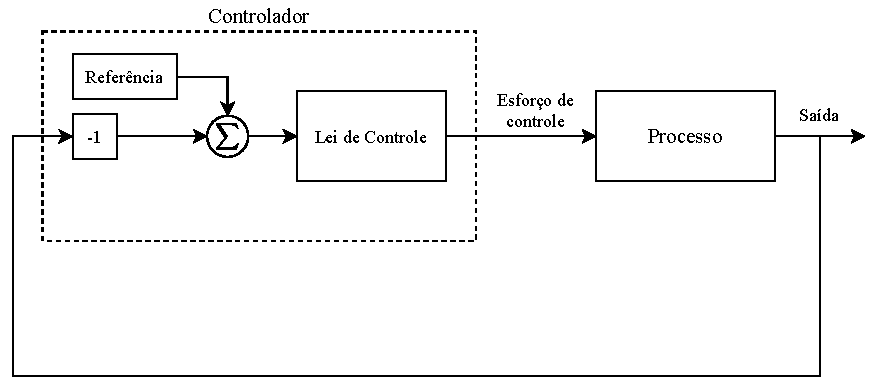
\includegraphics[width=1\linewidth]{diag/introducao/pdf/controleMF}
	\captionof{figure}[Sistema de controle em malha fechada]{Sistema de controle em malha fechada.}
	\label{fig:introducao:controleMF}
	\vspace{\onelineskip}
\end{minipage}

No entanto, outros critérios devem ser considerados no controle de sistemas de dinâmica complexa (possuem múltiplas entradas e saídas e que estejam sujeitos a limitações operacionais). Por exemplo, considerando-se a determinação das forças $ F(t) $ a serem impostas sob uma aeronave para que um dado ponto de chegada seja atingido, de forma que sejam evitadas zonas proibitivas, ao mesmo tempo em que minimiza-se o gasto de combustível da aeronave, conforme observado na Figura \ref{fig:introducao:aeronaveControleOtimo}. Vale ressaltar que, nesse caso, os perfis de aceleração $ a(t) $, de velocidade $ v(t) $, e de posição $ P\big(x(t), y(t)\big) $ da aeronave devem ser também determinados. O Controle Ótimo (CO) é uma das ferramentas que possibilita a resolução de problemas desse tipo. 

\noindent	
\begin{minipage}{\textwidth}
	\vspace{\onelineskip}
	\centering
	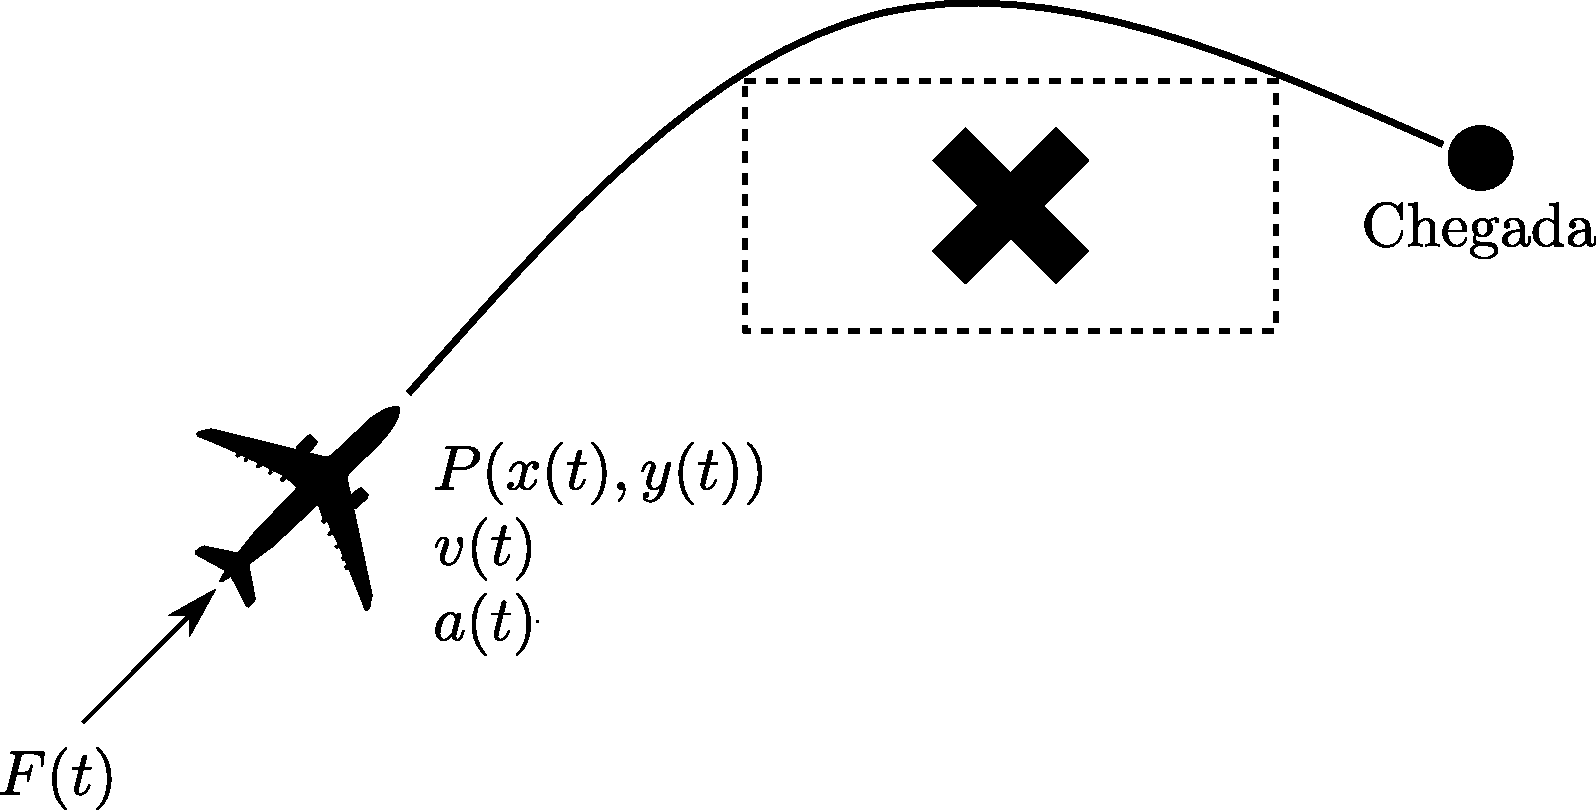
\includegraphics[width=0.7\linewidth]{draw/introducao/pdf/aviaoControleOtimo}
	\captionof{figure}[Trajetória ótima a ser percorrida por uma aeronave para que um determinado ponto de chegada seja atingido]{Trajetória a ser percorrida por uma aeronave para que um determinado ponto de chegada seja atingido, de forma que seja evitada uma dada zona proibitiva, nesse caso assinalada com um $ \times $, ao mesmo tempo em que minimiza-se o gasto de combustível da aeronave. O estabelecimento desta dessa trajetória depende da determinação dos perfis de aceleração $ a(t) $, de velocidade $ v(t) $, e de posição $ P\big(x(t), y(t)\big) $ da aeronave.}
	\label{fig:introducao:aeronaveControleOtimo}
	\vspace{\onelineskip}
\end{minipage}

O CO consiste em um conjunto de métodos que possibilita a determinação dos perfis de controle que conduzem à minimização (ou maximização) de um dado índice de desempenho, garantindo, simultaneamente, que restrições operacionais e dinâmicas sejam satisfeitas \cite{kirk_optimal_2004, becerra_optimal_2008, kelly_introduction_2017}. 

\todo[inline, color=pink, size=normalsize]{Aplicações reais do controle ótimo (vacinação contra COVID-19 e manobrabilidade de satélite)}

As origens do CO remontam ao começo do século XVII, porém foi a partir da década de 50, com o advento do computador digital, que o CO passou a ser utilizado no campo da engenharia \cite{bryson_optimal_1996}. Desde então, o CO têm sido empregue na resolução de problemas associados ao controle de processos industriais, à bioengenharia, à economia, à gestão, à robótica, e à engenharia aeroespacial \cite{becerra_optimal_2008}.  

Um exemplo que mostra o quão vantajoso pode ser o emprego do CO é apresentado em \citeonline{kang_pseudospectral_2007}, que relata o sucesso de uma manobra performada pela Estação Espacial Internacional (\textit{International Space Station} ou ISS) no dia 3 de março de 2007. Combinando-se um controlador clássico e um gerador de trajetórias baseado nas teorias de CO, foi possível que a ISS realizasse um giro de 180$^{\circ}$ sem que qualquer combustível fosse gasto. Para realização de manobras desse tipo a ISS dispõe de propulsores movidos à combustível e de giroscópios que consomem a energia elétrica fornecida pelos painéis solares da estação espacial (ver a Figura \ref{fig:introducao:giroscopios}). O uso exclusivo dos giroscópios na reorientação da ISS possibilitou uma economia de, aproximadamente, 1 milhão de dólares em combustível.

\noindent	
\begin{minipage}{\textwidth}
	\vspace{\onelineskip}
	\centering
	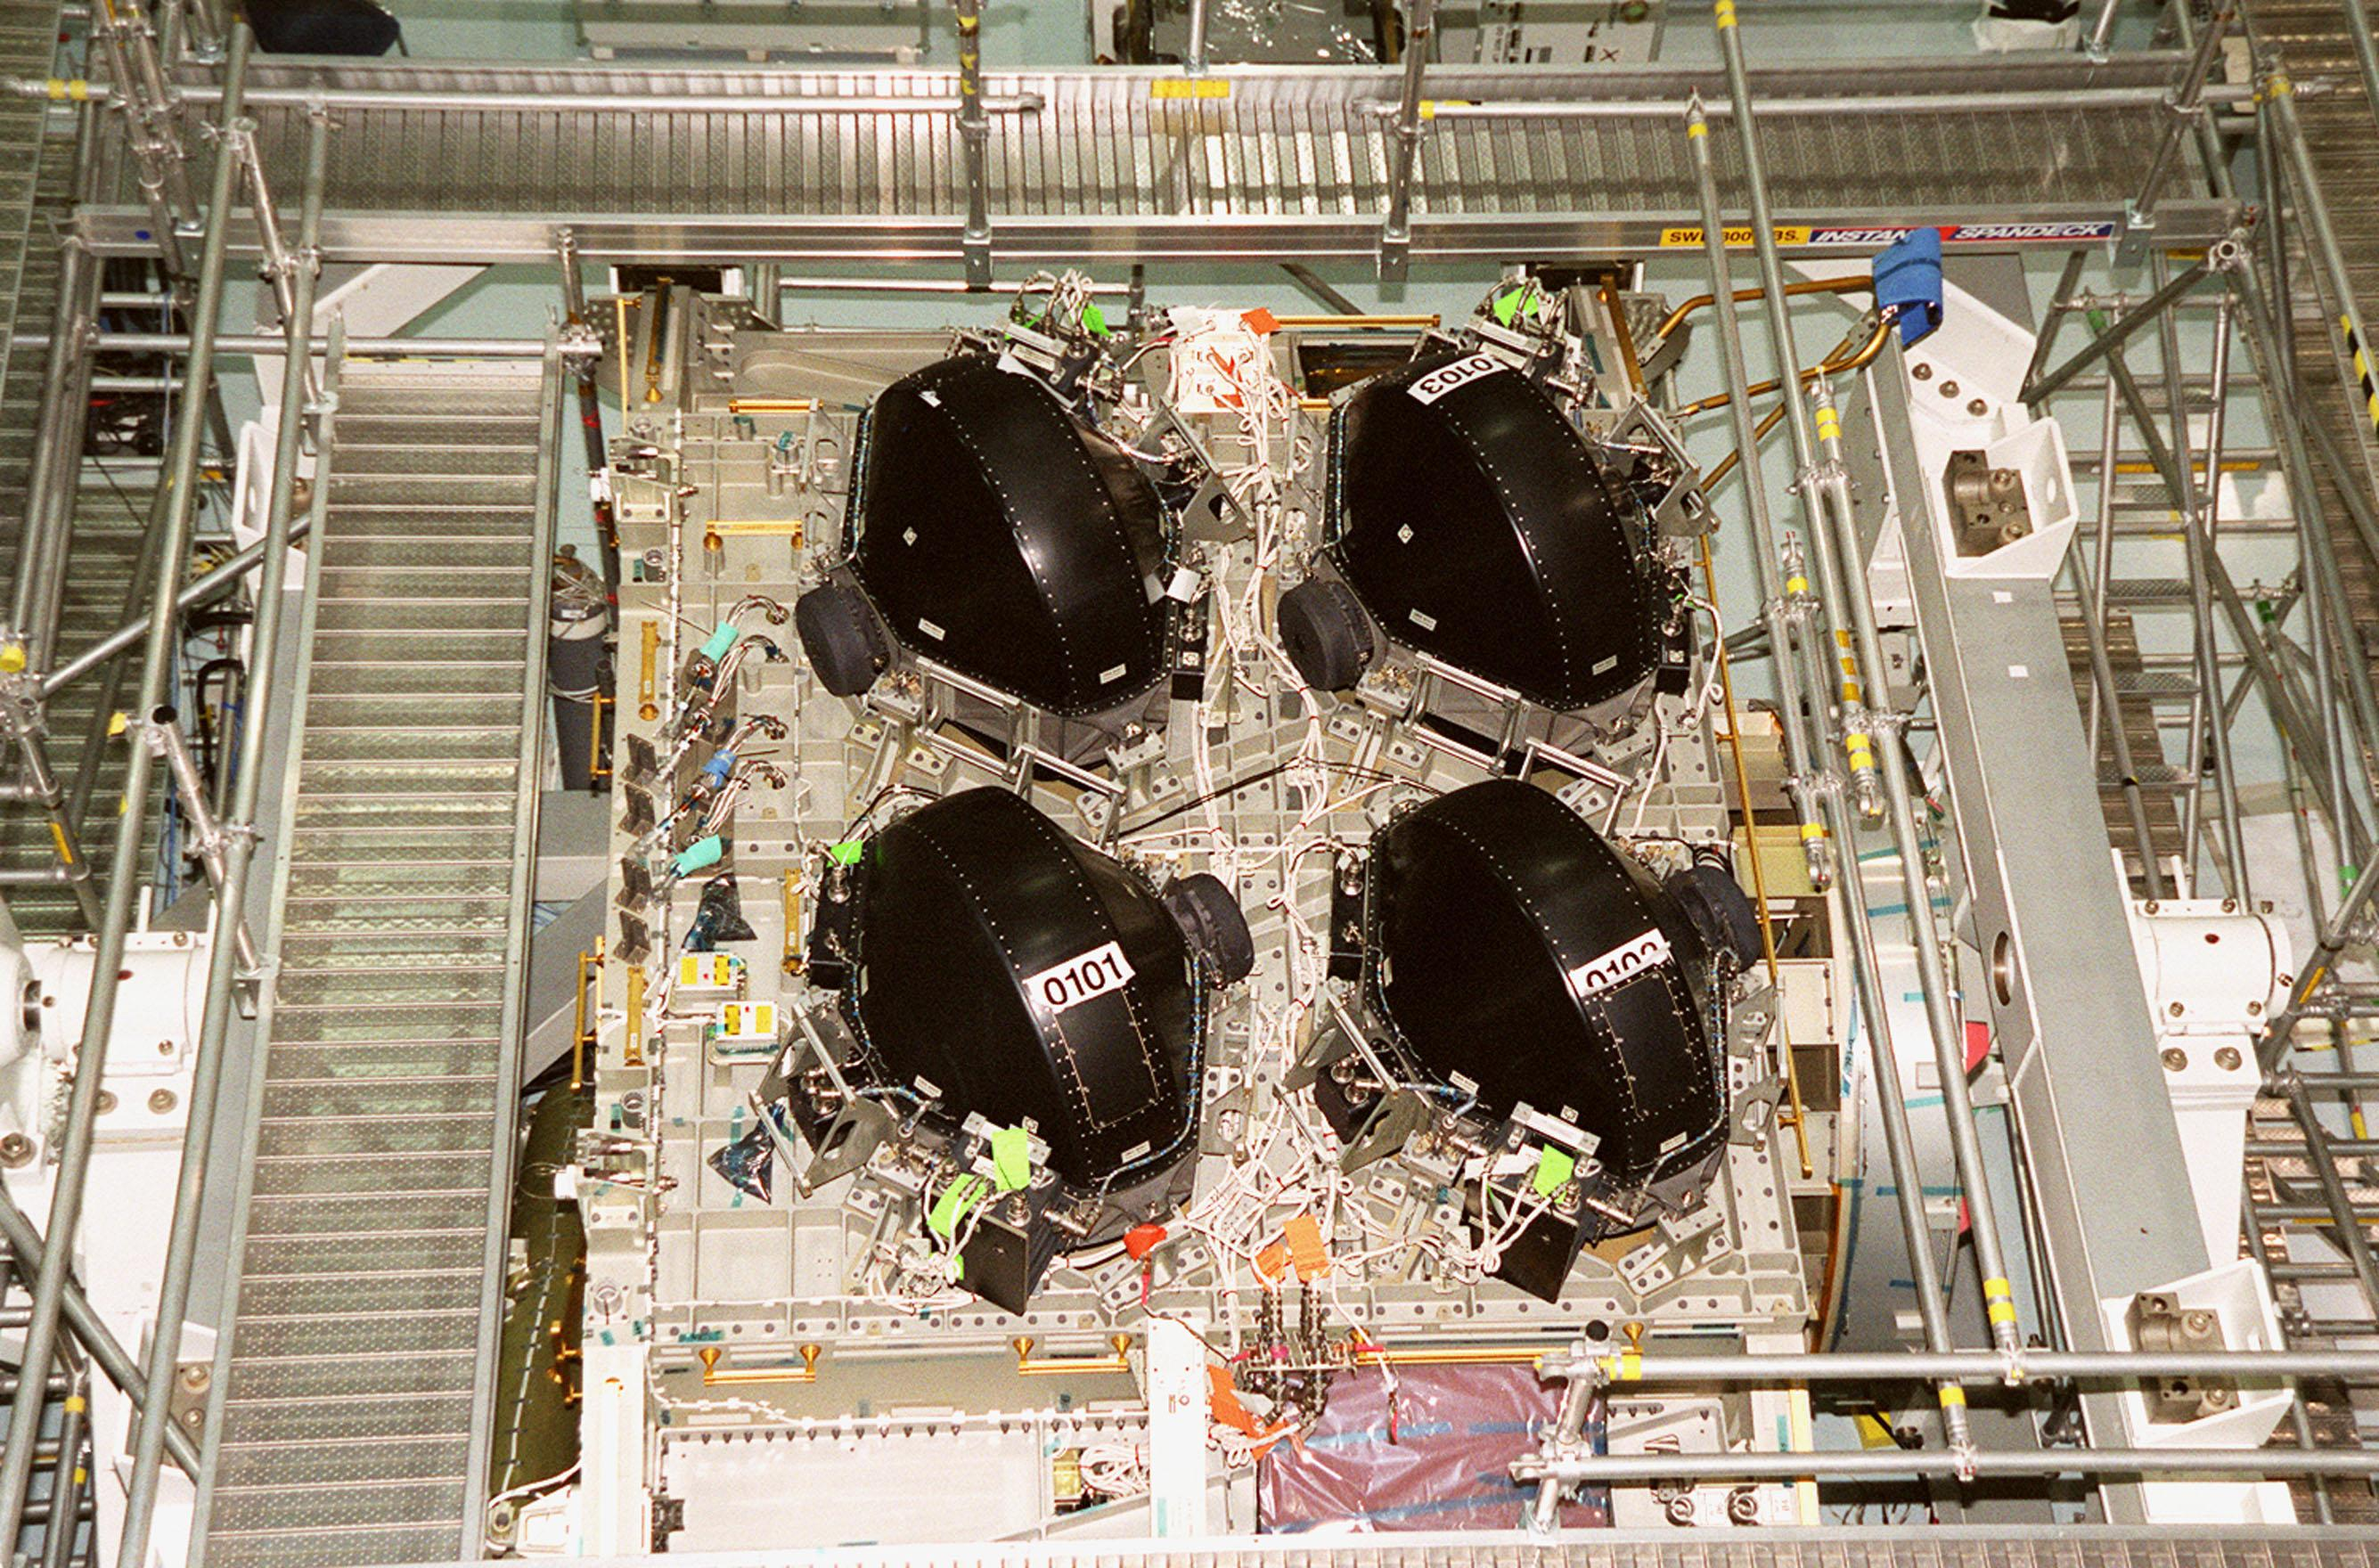
\includegraphics[width=0.8\linewidth]{fig/introducao/giroscopiosISS}
	\captionof{figure}[Giroscópios da ISS]{Giroscópios da ISS (Fonte: \url{https://cutt.ly/djEW0PD}).}
	\label{fig:introducao:giroscopios}
	\vspace{\onelineskip}
\end{minipage}

O CO pode ser empregado até mesmo no tratamento de questões que envolvem a gestão da saúde pública, como mostrado em \citeonline{libotte_determination_2020}. Em novembro de 2019, um novo vírus chamado COVID-19 (\textit{Coronavirus disease 2019}), emergiu da China e rapidamente se espalhou pelo mundo conforme observado na Figura \ref{fig:introducao:espalhamentoCOVID} \cite{libotte_determination_2020}. Até janeiro de 2020 o vírus infectou mais de 90 milhões de pessoas pelo mundo e fez 2 milhões de vítimas, 200 mil delas no Brasil \cite{dong_interactive_2020}. Apesar das medidas de distanciamento social serem uma forma efetiva de reduzir o espalhamento da COVID-19, somente uma companha de vacinação será capaz de frear a disseminação da doença. Nesse contexto, uma estratégia de vacinação formulada a partir do emprego de técnicas de CO e Otimização Heurística é proposta em \citeonline{libotte_determination_2020}. A estratégia em questão visa não só a minimização do número de indivíduos infectados, mas também do número de doses utilizadas. Os autores demonstraram que o  emprego dessa estratégia levaria a uma diminuição de aproximadamente 10 vezes no número de indivíduos infectados.

\noindent	
\begin{minipage}{\textwidth}
	\vspace{\onelineskip}
	\centering
	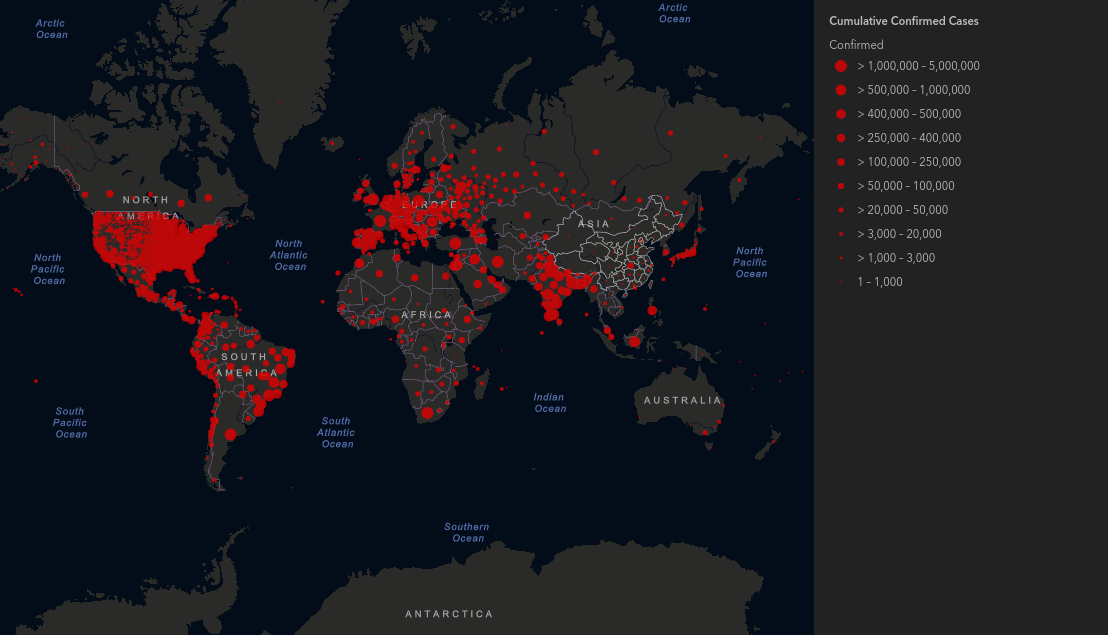
\includegraphics[width=1\linewidth]{fig/introducao/mapaCovid}
	\captionof{figure}[Mapa que mostra o número de indivíduos infectados pela COVID-19 em várias regiões do mundo]{Mapa que mostra o número de indivíduos infectados pela COVID-19 em várias regiões do mundo (Fonte: \url{https://cutt.ly/2jT37VO}).}
	\label{fig:introducao:espalhamentoCOVID}
	\vspace{\onelineskip}
\end{minipage}

\todo[inline, color=pink, size=normalsize]{Controle Ótimo computacional, a existência de pacotes computacionais para resolver problemas de controle ótimo e os pacotes que vou usar}

Como mencionado anteriormente, a teoria do CO passou a ser aplicada no campo da engenharia a partir da década de 50, com o advento do computador digital \cite{bryson_optimal_1996}. Desde então, PCOs cada vez mais complexos e práticos vem sendo abordados graças ao desenvolvimento da teoria de CO, à implementação de ferramentas de otimização mais eficientes e robustas, e ao aumento do poder computacional dos computadores pessoais \cite{biral_notes_2016}. Nesse contexto, diversos pacotes foram propostos para solução de PCOs, como o BOCOP \cite{saclay_bocop_2017}, o FALCON \cite{rieck_falconm_2020}, o GEKKO \cite{beal_gekko_2018}, o HamPath \cite{caillau_differential_2012}, o OpenOCL \cite{koenemann_openoclopen_2017}, o OptminTraj \cite{kelly_optimtraj_2018}, o OpenGoddard \cite{interstellar_technologies_inc_opengoddard_2020}, o Beluga \cite{rapid_design_of_systems_laboratory_beluga_2021}, o ICLOCS \cite{falugi_iclocs2_2018}, e o PSOPT \cite{becerra_psopt_2019}, apenas para citar alguns exemplos. 

\todo[inline, color=pink, size=normalsize]{Dificuldade em escolher um pacote que atenda às necessidades do usuário e se aplique de forma satisfatória ao seu problema}

A escolha de uma pacote, portanto, não é uma tarefa trivial diante de tantas possibilidades. Até mesmo a escolha das métricas a serem utilizadas na elaboração de um estudo comparativo entre os pacotes disponíveis consiste em um desafio, inclusive para usuários experientes \cite{bongartz_numerical_1997}. Além disso, não é somente com base no desempenho computacional que um dado pacote deve ser selecionado. É bastante importante que critérios referentes, à usabilidade, à documentação, às licenças, e ao suporte associados aos pacotes em análise sejam também considerados \cite{parejo_metaheuristic_2012}. 

\todo[inline, color=pink, size=normalsize]{Objetivos}

Diante desse contexto, o presente trabalho tem como objetivo central realizar um estudo comparativo entre pacotes computacionais desenvolvidos para resolução de problemas de Controle Ótimo. Para essa finalidade serão utilizados parâmetros relacionados ao esforço computacional, à qualidade das soluções obtidas, e à usabilidade associados a cada pacote. Como objetivos específicos ressaltam-se:	

\begin{itemize}
	\item Determinar um conjunto de estudos de caso e de métricas de desempenho e usabilidade, que possibilitem a elaboração de um estudo comparativo dos pacotes em análise;
	
	\item Definir qual dos métodos/pacotes avaliados é mais apropriado para resolução de cada tipo de PCO levando-se em conta a forma do índice de desempenho, a presença ou não de restrições nos estados e controles, a presença de arcos singulares, e o número de fases empregadas na formulação de cada PCO;
	
	\item Apresentar um estudo comparativo que sirva de guia para novos usuários dos pacotes avaliados.
\end{itemize}

\todo[inline, color=pink, size=normalsize]{Estrutura do trabalho}

O restante do texto se encontra organizado da seguinte maneira: No Capítulo \ref{sec:revisao} são estabelecidos alguns conceitos fundamentais acerca do CO, dos pacotes avaliados, e dos métodos numéricos nos quais os mesmos se baseiam. No Capítulo \ref{sec:metodologia} são apresentados os estudos de caso e as métricas de desempenho. No Capítulo \ref{sec:resultados} são apresentados os resultados obtidos considerando estudos de caso com diferentes características. Por fim, no Capítulo \ref{sec:conclusoes} são apresentadas as conclusões advindas do desenvolvimento desse trabalho e algumas sugestões para trabalhos futuros.  

% REVISÃO BIBLIOGRÁFICA
\chapter{Revisão bibliográfica}
\label{sec:revisao}
Nesse capítulo são apresentados conceitos que servem de base para o desenvolvimento do presente trabalho. Inicialmente será brevemente abordada a história do Controle Ótimo para que, em seguida, o problema de Controle Ótimo seja definido. Em seguida, apresenta-se uma visão geral sobre os Métodos Diretos, empregados nos pacotes avaliados no presente trabalho. Por fim, esses pacotes são brevemente apresentados. 
\section{Uma breve história do Controle Ótimo}

\todo[inline, color=pink]{Histórico do Controle Ótimo}

O Controle Ótimo (CO) é um conjunto de métodos que possibilita a determinação das trajetórias de estados e controles que, quando impostas a um dado sistema dinâmico, garantem que as restrições operacionais associadas ao mesmo sejam satisfeitas, enquanto promovem a minimização (ou maximização) de um dado índice de desempenho \cite{kirk_optimal_2004, becerra_optimal_2008, kelly_introduction_2017}. As origens do CO remontam ao ano de 1697, quando Johann Bernoulli, professor de matemática da Universidade de Groningen, no norte da Holanda, publicou a solução do problema da braquistócrona \cite{sussmann_300_1997}, proposto por Galileo Galilei 59 anos antes \cite{bryson_optimal_1996}. Em 1696, Johann Bernoulli desafiou seus contemporâneos a resolver esse problema, que consiste na determinação da trajetória a ser percorrida por uma esfera que deve se mover entre dois pontos A e B, apenas sob a ação da gravidade, no menor tempo possível, conforme ilustrado na Figura \ref{fig:revisao:braquistocrona}. Soluções para o problema da braquistócrona foram propostas por Johan Bernoulli, Newton, Leibniz, l'Hopital e Jakob Bernoulli, irmão de Johan \cite{bryson_optimal_1996}.

\noindent	
\begin{minipage}{\textwidth}
	\vspace{\onelineskip}
	\centering
	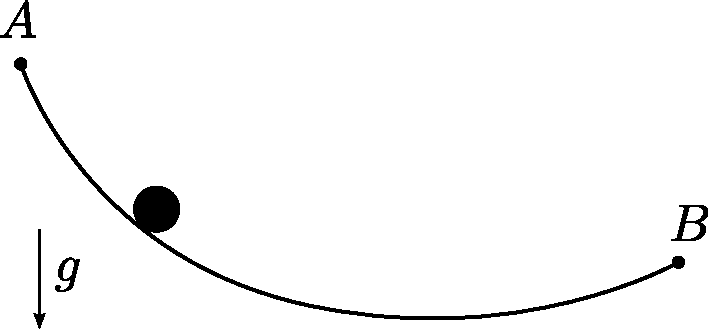
\includegraphics[width=0.5\linewidth]{draw/revisao/pdf/braq}
	\captionof{figure}[Representação do problema da braquistócrona]{Representação do problema da braquistócrona.}
	\label{fig:revisao:braquistocrona}
	\vspace{\onelineskip}
\end{minipage}

Pode-se dizer que o CO é uma extensão do Cálculo de Variações (CV), desenvolvido por Isaac Newton em 1685, e que buscava determinar o formato da ponta de um projétil que levasse à minimização do arrasto aerodinâmico. Em 1744, Leonard Euler publicou um livro intitulado \textit{\textcolor{red}{Arthur, colocar aqui o nome do livro em inglês, por favor}}, no qual são apresentadas as bases para o desenvolvimento teórico do CV. Euler e Jean Louis Lagrange trocaram cartas a respeito desse livro e juntos desenvolveram a equação de Euler-Lagrange. Esta descreve a condição necessária de primeira ordem associada à solução de um problema de CV \cite{bryson_optimal_1996}.

Em 1836, Willian Rowan Hamilton publicou um trabalho aplicando o CV ao projeto de sistemas mecânicos a partir da minimização da força exercida pelos mesmos. As soluções obtidas por Hamilton foram baseadas na resolução de duas equações diferenciais, e por esse motivo, o autor foi criticado, em 1838, por Karl Gustav Jacob Jacobi, que afirmou que apenas uma equação bastaria. A partir do trabalho desses dois autores desenvolveu-se a equação de Hamilton-Jacobi, que serviu de base para que Richard Bellman propusesse a programação dinâmica mais de 100 anos depois \cite{bryson_optimal_1996}. 

Com base no trabalho desenvolvido por Karl Wilhelm Theodor Weierstrass no final do século XIX, Oskar Bolza e Gilbert A. Bliss associaram ao CV o rigor matemático que o acompanha até os dias atuais. A partir do trabalho atribuído a Bolza e Bliss, McShane desenvolveu, em 1939, um método para resolução de problemas de CV, que seria estendido por Pontryagin anos depois dando origem ao princípio do mínimo de Pontryagin. Em 1957, Placido Cicala escreveu uma monografia a respeito do emprego do CV no desenvolvimento de projetos de engenharia e, em 1963, Derek Lawden foi o primeiro a empregar o CV na determinação de trajetórias para veículos espaciais \cite{bryson_optimal_1996}. 

No entanto, é importante salientar que o Controle Clássico também serviu de base para o desenvolvimento do CO. O Controle Clássico consiste num conjunto de metologias normalmente baseadas em procedimentos a partir dos quais determinam-se os ganhos de um controlador para que a implementação do mesmo leve a uma resposta em malha fechada satisfatória \cite{bryson_optimal_1996}.

Durante e após a Segunda Guerra Mundial, diversos métodos baseados nas transformadas de Laplace e Fourier, e nas variáveis complexas, foram desenvolvidos para que o desempenho e a estabilidade de sistemas de controle em malha fechada fossem previstos. Com o surgimento dessas técnicas, critérios quantitativos passaram a ser definidos no domínio da frequência, como os ganhos de margem e de fase, e no domínio do tempo, como o tempo de acomodação e o máximo sobressinal (ou \textit{overshoot}) associados à resposta do sistema a uma entrada do tipo degrau \cite{bryson_optimal_1996}.

A utilização da integral do quadrado do erro (ISE) na sintonização de um controlador em malha fechada foi proposta pela primeira vez por Newton, Gould e Kaiser em 1957. Já em 1961, Chang propôs o projeto de um controlador com base em restrições associadas à integral do quadrado da ação de controle. Em 1960, Kalman estabeleceu os conceitos de variáveis de estado e controle, que são largamente utilizadas no CO, assim como um índice de desempenho integral computado a partir das magnitudes dos controles e erros. Kalman mostrou, empregando o CV, que os controles poderiam ser determinados a partir de uma realimentação linear das variáveis de estado. Posteriormente, o controlador proposto por Kalman seria chamado de Regulador Linear Quadrático (LQR) \cite{bryson_optimal_1996}. 

Por fim, é preciso ressaltar que o CO possui também origens na Programação Não Linear (PNL), desenvolvida logo após a Segunda Guerra Mundial. Esta consiste na otimização de uma dada função objetivo a partir da determinação de parâmetros (ou variáveis de projeto), sujeitos a restrições de igualdade e desigualdade. Caso o perfil de controle seja aproximado por um conjunto finito de pontos no tempo, é possível que a PNL seja empregada na determinação do valor assumido pelo esforço de controle em cada um desses pontos, de forma que o problema de OC inicialmente proposto seja resolvido de forma numérica \cite{bryson_optimal_1996}. Esse abordagem será discutida em detalhes mais adiante uma vez que serve de base para o desenvolvimento do presente trabalho.  

\section{O problema de Controle Ótimo}

%\todo[inline, color=pink]{Definição do Controle Ótimo}
%
%O CO consiste em um conjunto de metodologias que possibilita a determinação de perfis de controles e estados, ou de ganhos de controladores em malha fechada, que minimizem um dado índice de desempenho de forma que sejam respeitadas restrições diferenciais referentes à dinâmica do sistema a ser controlado \cite{bryson_optimal_1996}. Além das restrições dinâmicas, é importante salientar que, em alguns casos, é preciso que sejam consideradas restrições de caminho, associadas à evolução temporal dos estados e/ou controles, restrições terminais, relacionadas aos valores assumidos pelos estados ao fim da trajetória, e restrições associadas especificamente às amplitudes dos estados e/ou controles \cite{becerra_optimal_2008}.

\todo[inline, color=pink]{O Problema de Controle Ótimo}

O problema de Controle Ótimo (PCO) é definido de acordo com a formulação de Bolza \cite{becerra_optimal_2008}:
%
\begin{subequations}
\begin{equation}
	\label{eq:revisao:PCO}
		\underset{\mathbf{u}(t)}{\text{min}} \; J = \varphi \big( \mathbf{x}(t_f), t_f \big) + \int_{t_0}^{t_f} L \big( \mathbf{x}(t), \mathbf{u}(t), t \big) \, dt
\end{equation}
\vspace{-0.4cm}
\begin{equation}
		\mathbf{\dot{x}}(t) = \mathbf{f} \big( \mathbf{x}(t), \mathbf{u}(t), t \big), \; \mathbf{x}(t_0) = \mathbf{x_0} 
\end{equation}
\end{subequations}
%
sendo $ \mathbf{x}(t) $ e $ \mathbf{u}(t) $, respectivamente, os vetores de estados e controles do sistema, $ t $ a variável temporal, $ t_0 $ e $ t_f $ os tempo inicial e final, respectivamente, $ J $ o funcional a ser minimizado (ou maximizado), também chamado índice de desempenho ou função objetivo, $ \varphi $ a função de custo terminal, também conhecida como função de Mayer, $ L $ a função de custo de caminho, também intitulada função de Lagrange, $ \mathbf{f} $ o sistema de equações que descreve a dinâmica do sistema, tipicamente no espaço de estados, e $ \mathbf{x_0} $ a condição inicial atribuída a $ \mathbf{x}(t) $. Considera-se que estão associados à formulação de $ \mathbf{f} $ $ n $ estados e $ m $ controles, de forma que:
%
\begin{subequations}
\begin{equation}
\mathbf{x}(t) = \begin{bmatrix} x^{(1)}(t) & x^{(2)}(t) & \dots & x^{(n)}(t) \end{bmatrix}^T
\end{equation}
\vspace{-0.5cm}
\begin{equation}
\mathbf{u}(t) = \begin{bmatrix} u^{(1)}(t) & u^{(2)}(t) & \dots & u^{(m)}(t) \end{bmatrix}^T
\end{equation}
\end{subequations}

Vale ressaltar que caso $ t_0 $ e $ t_f $ não sejam previamente estabelecidos, devem ser determinados por meio da resolução do PCO, e nesse caso, restrições associadas aos limites de $ t_0 $ e $ t_f $ devem ser consideradas. Além disso, uma vez determinado $ \mathbf{u}(t) $, é possível que, de posse de $ \mathbf{x_0} $, determinem-se a trajetórias dos estados com base na computação de $ \mathbf{f} \big( \mathbf{x}(t), \mathbf{u}(t), t \big) $.

A formulação de um PCO pode incluir restrições associadas às amplitudes dos estados e/ou controles, que serão referenciadas ao longo do texto como restrições laterais: 
%
\begin{subequations}
\begin{equation}
\mathbf{x_L} \leq \mathbf{x}(t) \leq \mathbf{x_U} 
\end{equation}
\vspace{-0.75cm}
\begin{equation}
\mathbf{u_L} \leq \mathbf{u}(t) \leq \mathbf{u_U}
\end{equation}
\end{subequations}
sendo os índices $ L $ e $ U $ utilizados na representação dos limites inferiores e superiores dos estados e controles. Além disso, podem-se considerar restrições de caminho, associadas à evolução temporal dos estados e/ou controles, 
%
\begin{equation}
	\mathbf{c}(\mathbf{x}(t), \mathbf{u}(t), t) \leq \mathbf{0} 
\end{equation}
%
e restrições terminais, relacionadas aos valores assumidos pelos estados ao fim da trajetória,
%
\begin{equation}
	{\bm \psi}(\mathbf{x}(t_f), t_f) \leq \mathbf{0} 
\end{equation}
%
sendo $ \mathbf{c} $ e $ {\bm \psi} $, funções quaisquer.  

Um PCO pode ser formulado, por exemplo, para que os perfis de velocidade $ x_2(t) $ e posição $ x_1(t) $ de um carro que corre sobre um trilho sejam determinadas. Para tanto, é necessário que seja também computado o perfil da força $ u(t) $ exercida sobre o carro, representado nesse caso como um ponto de massa. Pode-se considerar ainda que o tempo despendido na transposição de 10 m de trilho, e a força empregada na realização desse movimento devam ser minimizados. Supondo que, devido aos materiais utilizados na construção do aparato em questão, e do motor que movimenta carro, haja limitações na velocidade e na potência associadas à movimentação do mesmo, pode-se determinar $ x_1(t) $, $ x_2(t) $, $ u(t) $ e $ t_f $ a partir da resolução do PCO introduzido como segue:
%
\begin{subequations}
\begin{equation}
\label{eq:revisao:PCOExemplo}
\underset{\mathbf{u}(t), \, t_f}{\text{min}} \; J = t_f + \int_{0}^{t_f} u^2(t) \, dt
\end{equation}
\vspace{-0.3cm}
\begin{equation}
\dot{x}_1(t) = x_2(t), \; x_1(0) = 0 \text{ m} 
\end{equation}
\vspace{-0.6cm}
\begin{equation}
\dot{x}_2(t) = u(t), \; x_2(0) = 0 \text{ m$/$s} 
\end{equation}
\vspace{-0.6cm}
\begin{equation}
-2 \text{ m$/$s} \leq x_2(t) \leq 2 \text{ m$/$s} 
\end{equation}
\vspace{-0.6cm}
\begin{equation}
-10 \text{ N} \leq u(t) \leq 10 \text{ N} 
\end{equation}
\vspace{-0.6cm}
\begin{equation}
-15 \text{ W} \leq u(t) \, x_2(t) \leq 15 \text{ W} 
\end{equation}
\vspace{-0.6cm}
\begin{equation}
x_1(t_f) = 10 \text{ m}
\end{equation}
\end{subequations}

A formulação do PCO apresentada contempla uma restrição de caminho vinculada à potência empregue na movimentação do carro, uma restrição terminal relacionada à posição final do mesmo, e restrições associadas a limitações na velocidade $ x_2(t) $ do carro e na força $ u(t) $ que atua sob o mesmo. 

\todo[inline, color=pink]{Conceitos Gerais}

\section{Conceitos Gerais}

A presente seção tem por objetivo apresentar uma série de conceitos importantes para o estudo do PCO. Neste caso, são avaliadas características que abrangem uma equação algébrico-diferencial - EAD (resultante da aplicação de otimalidade para o PCO), bem como aspetos relacionados com a presença de restrições \cite{bryson_optimal_1996,lobato2004}.

\begin{itemize}

\item Arcos Singulares: arcos onde a matriz de derivadas segundas da função  Hamiltoniano com relação às variáveis de controle é singular. Neste contexto, alguns PCOs são definidos a partir de domínios nos quais podem ser observadas regiões em que a condição estacionária $ \mathbf{H_{u}} = \partial \mathit{H} / \partial u $ é satisfeita ao mesmo tempo em que a matriz Hessiana $ \mathbf{H_{uu}} = \partial^2 \mathit{H} / \partial u^2 $ associada ao Hemiltoniano $ \mathit{H} $ é singular. Essas regiões são chamadas arcos singulares, e nelas, $ u(t) $ não pode ser unicamente definido pela condição estacionária, sendo necessário impor que as derivadas temporais de $ \mathbf{H_{u}} $ sejam nulas ao longo do arco. Adversidades numéricas podem ser enfrentadas caso métodos computacionais sejam empregados na resolução de PCOs que possuam arcos singulares \cite{betts_practical_2001, becerra_optimal_2008}.

Como exemplos de PCOs que apresentam arcos singulares pode-se citar: 
%
\begin{itemize}
	\item Determinação de trajetórias ótimas para foguetes de sondagem, que realizam voos suborbitais para coleta de dados utilizados em estudos meteorológicos e astronômicos \cite{nasa_what_2004};
	
	\item Estabelecimento do curso de uma aeronave que realiza voos periódicos para minimização do gasto de combustível \cite{speyer_periodic_1996};
	
	\item Estudo da influência do fenômeno meteorológico \textit{wind shear}, que consiste na variação brusca da direção e/ou velocidade do vento, no pouso de uma aeronave \cite{anac_wind_2018}.
\end{itemize}

\item Condição de Canto: ponto onde ocorre descontinuidade no perfil de controle ou na inclinação das trajetórias das variáveis de estado. 

\item EAD com Índice Superior e Redução de Índice: são as equações com índice maior do que $1$. O índice diferencial é o número mínimo de vezes que o sistema de equações algébrico-diferenciais ou parte dele deve ser diferenciado com relação ao tempo para determinar transformá-lo em um puramente diferencial. Este conceito representa uma medida da dificuldade de solução de sistema de EADs, decorrente de mau condicionamento, instabilidade, singularidade e má convergência. Do ponto de vista da solução numérica é desejável que o índice das EADs seja o menor possível devido à dificuldade associada na solução deste em comparação com a solução de equações diferenciais ordinárias com rigidez numérica. Entretanto,
esta redução obtida através da simples diferenciação das restrições pode não satisfazer as restrições originais de maneira exata, com sérias implicações quando elas envolvem propriedades físicas importantes. Portanto, devem ser consideradas formas de reintroduzir restrições perdidas no sistema, chamadas invariantes.

\item Eventos: pontos de junção entre os arcos sujeitos a restrições e os arcos sem
restrições.

\item Funções Identificadoras de Fase: relação matemática obtida a partir da aplicação da condição de otimalidade em um PCO e que tem por finalidade indicar a ativação o não de uma restrição. Um caso particular e de grande interesse é quando a variável de controle aparece linearmente na função Hamiltoniano. 

\end{itemize}

\todo[inline, color=pink]{Métodos Diretos}

\section{Métodos Diretos}

Os métodos empregados na resolução de PCOs podem ser divididos em duas principais categorias: os Métodos Indiretos e os Métodos Diretos. Os Métodos Indiretos se baseiam na resolução das condições necessárias de otimalidade associadas ao PCO. A formulação dessas condições depende da definição do Hamiltoniano $\mathit{H} \big( \mathbf{x}(t), \mathbf{u}(t), {\bm \lambda}(t), t \big)$: 
%
\begin{equation}
	\mathit{H} \big( \mathbf{x}(t), \mathbf{u}(t), {\bm \lambda}(t), t \big) = L \big( \mathbf{x}(t), \mathbf{u}(t), t \big) + {\bm \lambda}^T(t) \; \mathbf{f} \big( \mathbf{x}(t), \mathbf{u}(t), t \big)
\end{equation}
%
em que $ {\bm \lambda}(t) $ são os multiplicadores de Lagrange, também conhecidos como co-estados ou variáveis adjuntas. Assim sendo, as condições de otimalidade, ou equações de Euler-Lagrange, são introduzidas como segue \cite{becerra_optimal_2008}.
%
\begin{subequations}
\begin{equation}
	\label{eq:revisao:condicoesOtimalidade}
		{\bm \dot{ \bm \lambda}}^T(t) = - \frac{\partial \mathit{H} \big( \mathbf{x}(t), \mathbf{u}(t), {\bm \lambda}(t), t \big)}{\partial \mathbf{x}(t)}
\end{equation}
\vspace{-0.2cm}
\begin{equation}
	{\bm \lambda}^T(t_f) = \frac{\partial \varphi \big( \mathbf{x}(t_f), t_f \big)}{\partial \mathbf{x}(t)} \Biggr|_{t = t_f}
	\end{equation}
\begin{equation}
\label{eq:revisao:condicoesOtimalidadeb}
		\frac{\partial \mathit{H} \big( \mathbf{x}(t), \mathbf{u}(t), {\bm \lambda}(t), t \big)}{\partial \mathbf{u}(t)} = \mathbf{0}
\end{equation}
\end{subequations}

Apesar das soluções obtidas por meio dos Métodos Indiretos serem comumente bastante acuradas, pode ser consideravelmente difícil, a depender do PCO em análise, formular as condições necessárias de otimalidade, algo que um usuário com pouco conhecimento da teoria do CO dificilmente seria capaz de fazer. Além disso, o sucesso dos métodos numéricos empregados na resolução do sistema descrito pela Eqs. \eqref{eq:revisao:condicoesOtimalidade}-\eqref{eq:revisao:condicoesOtimalidadeb} depende fortemente das estimativas iniciais atribuídas a $ {\bm \lambda}(t) $, que não podem ser determinados de forma intuitiva, uma vez que não possuem significado físico \cite{betts_practical_2001}. 

Já os Métodos Diretos são baseados na discretização dos estados e controles, de forma que a resolução do PCO se dê a partir da determinação dos valores atribuídos aos mesmos em pontos específicos da trajetória, denominados nós (ou pontos) de colocação, conforme observado na Figura \ref{fig:revisao:discretizacao}. Mais de 90\% dos pacotes computacionais desenvolvidos para a resolução de PCOs são baseados nos Métodos Diretos. Essa popularidade se deve à existência de inúmeros pacotes robustos e bem estabelecidos para solução de um problema de programação não linear (PPNL), capazes de lidar de forma simples e direta com restrições de igualdade e desigualdade, e que não requerem que as equações associadas aos co-estados sejam fornecidas pelo usuário \cite{biral_notes_2016}. 

Uma vez que os estados, os controles, a função objetivo e as restrições associadas à dinâmica do PCO, tenham sido discretizados de forma que:
%
\begin{subequations}
\begin{equation}
t \rightarrow t_0, \, \dots, \, t_k, \, \dots, \, t_{M} 
\end{equation}
\vspace{-0.85cm}
\begin{equation}
\mathbf{x}(t) \rightarrow \mathbf{x}_0, \, \dots, \, \mathbf{x}_k, \, \dots, \, \mathbf{x}_{M}
\end{equation}
\vspace{-0.75cm}
\begin{equation}
\mathbf{u}(t) \rightarrow \mathbf{u}_0, \, \dots, \, \mathbf{u}_k, \, \dots, \, \mathbf{u}_{M}
\end{equation}
\end{subequations}
%
sendo $ \xi_k $ o valor atribuído à variável $ \xi $ no nó de colocação $ k $, é possível que o PCO em análise seja tratado como um problema de otimização clássica, mais especificamente um PPNL. Cabe ressaltar que $ M $ é o índice atribuído ao último nó de colocação, localizado em $ t = t_f $, e que, assumindo $ N $ como sendo o número de nós de colocação, tem-se $ M = N - 1 $. O processo de conversão de um PCO em um PPNL é conhecido como transcrição \cite{kelly_introduction_2017}. 

\begin{minipage}{\textwidth}
	\vspace{\onelineskip}
	\centering
	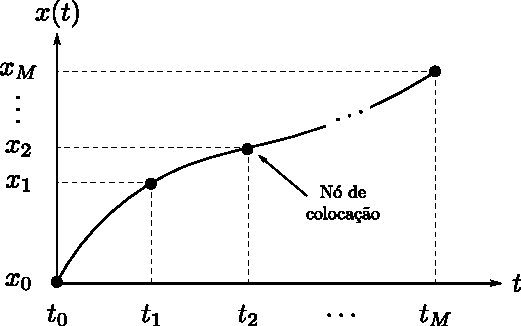
\includegraphics[width=0.7\linewidth]{draw/revisao/pdf/discretizacao}
	\captionof{figure}[Representação do processo de discretização em Métodos Diretos]{Representação do processo de discretização em Métodos Diretos.}
	\label{fig:revisao:discretizacao}
	\vspace{\onelineskip}
\end{minipage}

Os PPNLs são tipicamente formulados da seguinte maneira \cite{kelly_introduction_2017}, 
%
\begin{subequations}
\begin{equation}
\underset{\mathbf{z}}{\text{min}} \; F(\mathbf{z})
\end{equation}
\vspace{-0.75cm}
\begin{equation}
\mathbf{H}(\mathbf{z}) = \mathbf{0} 
\end{equation}
\vspace{-0.75cm}
\begin{equation}
\mathbf{G}(\mathbf{z}) \leq \mathbf{0}
\end{equation}
\vspace{-0.75cm}
\begin{equation}
\mathbf{z_L} \leq \mathbf{z} \leq \mathbf{z_U}
\end{equation} 
\end{subequations}
% 
em que $ F $ é o funcional a ser minimizado, $ \mathbf{H} $ e $ \mathbf{G} $ são os vetores de restrições de igualdade e desigualdade. Os limites inferior e superior associados ao vetor de variáveis de projeto (ou variáveis de decisão ou variáveis de busca) $ \mathbf{z} $, são denotados por $ \mathbf{z_L} $ e $ \mathbf{z_U} $ respectivamente.

Uma vez que o PPNL tenha sido resolvido e os valores atribuídos a $ \mathbf{x}(t) $ e $ \mathbf{u}(t) $ nos nós de colocação, denotados respectivamente por $ \mathbf{x}_k $ e $ \mathbf{u}_k $, tenham sido determinados, é possível que os perfis dos estados e controles sejam construídos a partir da interpolação de $ \mathbf{x}_k $ e $ \mathbf{u}_k $. A forma como se dá essa interpolação depende da metodologia empregada no processo de transcrição. As trajetórias dos controles, por exemplo, podem ser determinadas a partir da interpolação linear ou quadrática dos valores atribuídos a $ \mathbf{u}_k $, ao passo que as trajetórias dos estados podem ser especificadas com base na interpolação cúbica dos valores atribuídos a $ \mathbf{x}_k $ \cite{kelly_introduction_2017}. É possível ainda que as trajetórias de cada controle e estado sejam representadas por um único polinômio que percorra todos os nós de colocação \cite{becerra_psopt_2019}. 

%\subsection{Métodos de Colocação Direta}

%Como mencionado anteriormente, a transcrição de um PCO pode ser realizada de diversas maneiras. 

A implementação da maioria dos métodos de transcrição é baseada nos cinco passos listados a seguir:
%
\begin{enumerate}
	\item Discretização da integral associada à função objetivo;
	\item Discretização das restrições dinâmicas;
	\item Discretização das restrições de caminho, terminais e laterais;
	\item Solução do PPNL obtido a partir do processo de transcrição;
	\item Elaboração das trajetórias de estados e controles com base em $ \mathbf{x}_k $ e $ \mathbf{u}_k $ assumindo-se $ k = 0, \, 1, \, \dots, \, M $.
\end{enumerate}

A forma como cada uma dessas etapas será executada depende do método de transcrição adotado. Assim sendo, serão apresentados nas próximas seções alguns dos métodos mais comumente empregados na transcrição de PCOs.

\subsection{Colocação trapezoidal}
\label{sec:revisao:trap}

\todo[inline, color=pink]{Colocação trapezoidal}

A colocação trapezoidal é baseada na quadratura trapezoidal, empregada tanto na computação do integrando $L$ associada à função objetivo, quanto na discretização das restrições dinâmicas. Desta forma, assumindo-se $ h_k = t_{k+1} - t_k $, determina-se a integral de $L$ conforme a seguinte relação
%
\begin{equation}
	\label{eq:revisao:trap:integral}
	\int_{t_0}^{t_f} L \big( \mathbf{x}(t), \mathbf{u}(t), t \big) \, dt \approx \sum_{k=0}^{M-1} \frac{1}{2} h_k (L_k + L_{k+1})
\end{equation}
%
sendo $ L_k =  L \big( \mathbf{x}_k, \mathbf{u}_k, t_k \big)$ \cite{kelly_introduction_2017}.

Uma vez que os estados tenham sido discretizados é possível que as restrições diferenciais associadas à dinâmica do PCO sejam representadas por um conjunto de restrições algébricas. Para tanto, é necessário que as restrições dinâmicas sejam reescritas na forma integral e que a quadratura trapezoidal seja empregada \cite{kelly_introduction_2017}:
%
\begin{subequations}
\begin{equation}
\label{eq:revisao:trap:restricaoDinamica}
\mathbf{\dot{x}}(t) = \mathbf{f}(\mathbf{x}(t), \mathbf{u}(t), t)
\end{equation}
\vspace{-0.5cm}
\begin{equation}
\int_{t_k}^{t_{k+1}} \mathbf{\dot{x}}(t) \, dt = \int_{t_k}^{t_{k+1}} \mathbf{f}(\mathbf{x}(t), \mathbf{u}(t), t) \, dt
\end{equation}
\vspace{-0.25cm}
\begin{equation}
\mathbf{x}_{k+1} - \mathbf{x}_k \approx \frac{1}{2} h_k (\mathbf{f}_{k} + \mathbf{f}_{k+1})
\end{equation}
\end{subequations}

Assim sendo, $ M $ restrições de igualdade algébricas são formuladas a partir da equação anterior: 
%
\begin{equation}
	\mathbf{x}_{k+1} - \mathbf{x}_k - \frac{1}{2} \, h_k \, (\mathbf{f}_{k+1} + \mathbf{f}_k) = \mathbf{0}, \hspace{0.25cm} k = 0, \, \dots, \, M-1
\end{equation}
%
sendo $ \mathbf{f}_k = \mathbf{f}(\mathbf{x}_k, \mathbf{u}_k, t_k) $. Vale ressaltar que $ \mathbf{x}_k $ é uma variável de projeto, enquanto $ \mathbf{f}_k $ é obtido via avaliação do $ k $-ésimo nó de colocação  \cite{kelly_introduction_2017}.  

As restrições laterais, terminais e de caminho são incorporadas à formulação do PPNL a partir do momento em que são transformadas em restrições de igualdade e desigualdade. Infelizmente, uma vez que a resolução do PPNL depende apenas dos valores atribuídos aos estados e controles nos nós de colocação, somente nesses nós é possível garantir que as restrições serão de fato satisfeitas \cite{kelly_introduction_2017}. Assim sendo, as restrições associadas ao PCO podem ser transcritas da seguinte forma: 
%
\begin{subequations}
\begin{equation}
\mathbf{x_L} \leq \mathbf{x}(t) \leq \mathbf{x_U} \rightarrow \mathbf{x_L} \leq \mathbf{x}_k \leq \mathbf{x_U}, \; k = 0, \, \dots, \, M 
\end{equation}
\vspace{-0.85cm}
\begin{equation}
\mathbf{u_L} \leq \mathbf{u}(t) \leq \mathbf{u_U} \rightarrow \mathbf{u_L} \leq \mathbf{u}_k \leq \mathbf{u_U}, \; k = 0, \, \dots, \, M 
\end{equation}
\vspace{-0.7cm}
\begin{equation}
\mathbf{c}(\mathbf{x}(t), \mathbf{u}(t), t) \leq \mathbf{0} \rightarrow \mathbf{c}(\mathbf{x}_k, \mathbf{u}_k, t_k) \leq \mathbf{0}, \; k = 0, \, \dots, \, M
\end{equation}
\vspace{-0.7cm}
\begin{equation}
{\bm \psi}(\mathbf{x}(t_f), t_f) \leq \mathbf{0}  \rightarrow {\bm \psi}(\mathbf{x}_M, t_M) \leq \mathbf{0} 
\end{equation}
\end{subequations}
%
em que a condição inicial $ \mathbf{x_0} $ para o vetor de variáveis de estado é dado como:
%
\begin{equation}
	\mathbf{x}_k = \mathbf{x_0}, \hspace{0.25cm} k = 0 
\end{equation}
%

%As variáveis de projeto associadas ao PPNL advindo do processo de transcrição, considerando-se o caso geral em que $ t_0 $ e $ t_f $ devem ser determinados assim como $ \mathbf{u}_k $ e $ \mathbf{x}_k $, são introduzidas em \eqref{eq:revisao:variaveisPPNLTrap}
%%
%\begin{equation}
%	\label{eq:revisao:variaveisPPNLTrap}
%	\mathbf{z}^T = \begin{bmatrix} \mathbf{z_t}^T & \mathbf{z_x}^T & \mathbf{z_u}^T \end{bmatrix} 
%\end{equation}
%% 
%em que
%%
%\begin{equation}
%	\begin{gathered}
%		\mathbf{z_t}^T = \begin{bmatrix} t_0 & t_f \end{bmatrix} \\
%		\mathbf{z_x}^T = \begin{bmatrix} x^{(1)}_0 & x^{(1)}_1 & \dots & x^{(1)}_M & \dots & x^{(n)}_0 & x^{(n)}_1 & \dots & x^{(n)}_M \end{bmatrix} \\
%		\mathbf{z_u}^T = \begin{bmatrix} u^{(1)}_0 & u^{(1)}_1 & \dots & u^{(1)}_M & \dots & u^{(n)}_0 & u^{(n)}_1 & \dots & u^{(n)}_M \end{bmatrix} \\
%	\end{gathered}
%\end{equation}

Por fim, o emprego da colocação trapezoidal na avaliação do PCO descrito resulta no seguinte PPNL:
%
\begin{subequations}
\begin{equation}
\underset{\mathbf{u}_k, \, \mathbf{x}_k}{\text{min}} \; J = \varphi \big( \mathbf{x}_M, t_M \big) + \sum_{k=0}^{M-1} \frac{1}{2} h_k (L_k + L_{k+1}) \\
\end{equation}
\vspace{-0.1cm}
\begin{equation}
\mathbf{x}_{k+1} - \mathbf{x}_k - \frac{1}{2} \, h_k \, (\mathbf{f}_{k+1} + \mathbf{f}_k) = \mathbf{0}, \hspace{0.25cm} k = 0, \, \dots, \, M-1
\end{equation}
\vspace{-0.7cm}
\begin{equation}
\mathbf{x}(t_0) = \mathbf{x_0}
\end{equation}
\vspace{-0.7cm}
\begin{equation}
\mathbf{x_L} \leq \mathbf{x}_k \leq \mathbf{x_U}, \hspace{0.25cm} k = 0, \, \dots, \, M
\end{equation}
\vspace{-0.7cm}
\begin{equation}
\mathbf{u_L} \leq \mathbf{u}_k \leq \mathbf{u_U}, \hspace{0.25cm} k = 0, \, \dots, \, M
\end{equation}
\vspace{-0.7cm}
\begin{equation}
\mathbf{c}(\mathbf{x}_k, \mathbf{u}_k, t_k) \leq \mathbf{0} \hspace{0.25cm} k = 0, \, \dots, \, M \end{equation}
\vspace{-0.7cm}
\begin{equation}
{\bm \psi}(\mathbf{x}_M, t_M) \leq \mathbf{0} 
\end{equation}
\end{subequations}
%
em que $ t_0 $ e $ t_f $ são conhecidos. Não sendo esse o caso, $ t_0 $ e $ t_f $ devem ser determinadas de forma que as seguintes restrições sejam respeitadas:
%
\begin{subequations}
\begin{equation}
t_{0L} \leq t_0 \leq t_{0U}
\end{equation}
\vspace{-0.95cm}
\begin{equation}
t_{fL} \leq t_f \leq t_{fU}
\end{equation} 
\end{subequations}
%
sendo os limites inferiores de $ t_0 $ e $ t_f $ denotados por $ t_{0L} $ e $ t_{fL} $ e os superiores por $ t_{0U} $ e $ t_{fU} $, respectivamente. 

Uma vez que o PPNL tenha sido resolvido e que tanto $ \mathbf{x}_k $ quanto $ \mathbf{u}_k $ tenham sido determinados para $ k = 0, \, 1, \, \dots, \, M $, é possível que as trajetórias de estados e controles sejam elaboradas. A colocação trapezoidal é baseada na suposição de que os perfis de controle evoluem linearmente entre os nós de colocação e que podem, portanto, ser aproximados pela concatenação de polinômios (ou \textit{splines}) de primeira ordem, conforme ilustrado na Figura \ref{fig:revisao:controleLinear} \cite{kelly_introduction_2017}. 

\noindent	
\begin{minipage}{\textwidth}
	\vspace{\onelineskip}
	\centering
	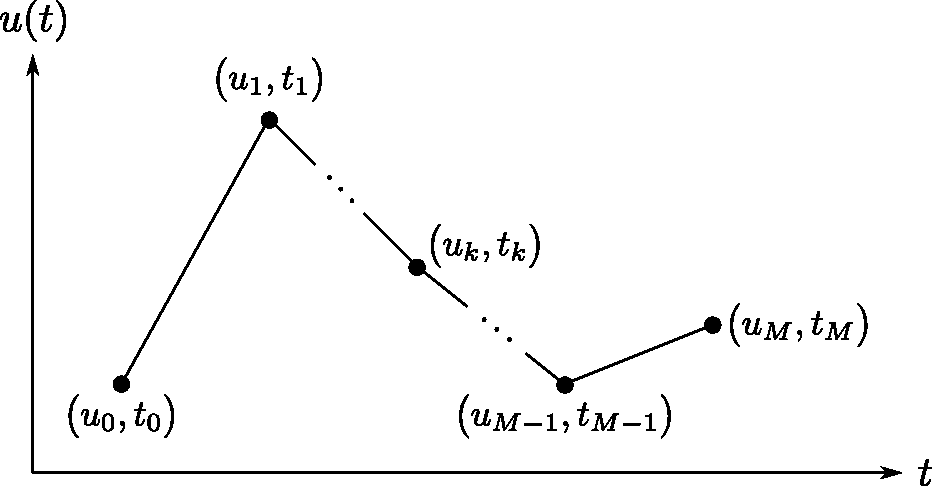
\includegraphics[width=0.8\linewidth]{draw/revisao/pdf/controleLinear}
	\captionof{figure}[Representação da trajetória considerando que os controles são lineares]{Representação da trajetória de controle $ u(t) $ considerando-se que os mesmos são lineares.}
	\label{fig:revisao:controleLinear}
	\vspace{\onelineskip}
\end{minipage}

Supondo que exista apenas uma variável de controle ($ \mathbf{u}(t) = u(t) $), pode-se determinar a mesma considerando uma aproximação linear por partes:
%
\begin{equation}
	\label{eq:revisao:uTrapInterp}
	u(t) = 
	\begin{cases} 
		a_1 \, t + b_1, & \mbox{se } t_0 \leq t \leq t_1 \\ 
		a_2 \, t + b_2, & \mbox{se } t_1 < t \leq t_2 \\ 
		\hspace{0.75cm} \vdots \\
		a_k \, t + b_k, & \mbox{se } t_{k-1} < t \leq t_{k} \\ 
		\hspace{0.75cm} \vdots \\
		a_M \, t + b_M, & \mbox{se } t_{M-1} < t \leq t_M 
	\end{cases}
\end{equation} 

Verifica-se que a $ k $-ésima \textit{spline} tem como extremos os pontos $ (t_{k-1}, u_{k-1}) $ e $ (t_k, u_k) $. Logo, os coeficientes $ a_k $ e $ b_k $ devem satisfazer:
%
\begin{subequations}
\begin{equation}
\label{eq:revisao:splineLinearEqs}
a_k \, t_{k-1} + b_k = u_{k-1}
\end{equation}
\vspace{-0.95cm}
\begin{equation}
a_k \, t_{k} + b_k = u_{k}
\end{equation}
\end{subequations}

Nota-se que a cada \textit{spline} estão associadas duas equações de forma que um sistema com $ 2M $ equações pode ser definido para que os coeficientes $ a_k $ e $ b_k $ sejam determinados para $ k = 1, \, 2, \, \dots, \, M $. 

Considerando, por exemplo, $ M = 3$ tem-se a seguinte estratégia de controle, conforme ilustrado na Figura \ref{fig:revisao:controleLinear4pontos}:
%
\begin{equation}
	u(t) = 
	\begin{cases} 
		a_1 \, t + b_1 , & \mbox{se } t_0 \leq t \leq t_1 \\ 
		a_2 \, t + b_2, & \mbox{se } t_1 < t \leq t_2 \\ 
		a_3 \, t + b_3, & \mbox{se } t_2 < t \leq t_3 
	\end{cases}
\end{equation} 

\noindent	
\begin{minipage}{\textwidth}
	\vspace{\onelineskip}
	\centering
	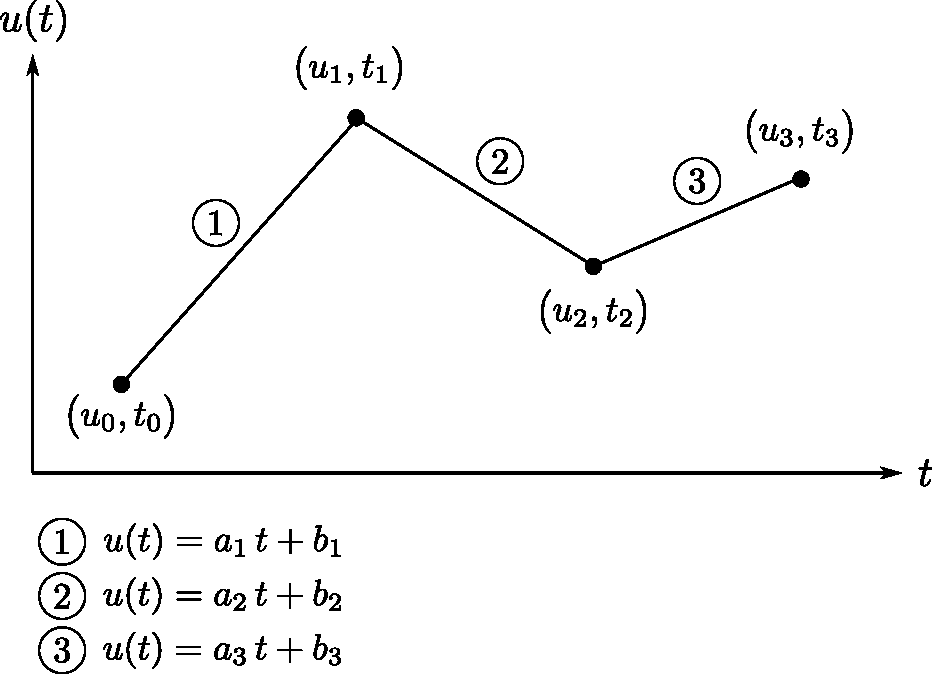
\includegraphics[width=0.7\linewidth]{draw/revisao/pdf/controleLinear4pontos}
	\captionof{figure}[Representação da trajetória do controle com quatro nós de colocação]{Representação da trajetória do controle $ u(t) $ considerando-se $ M = 3 $.}
	\label{fig:revisao:controleLinear4pontos}
	\vspace{\onelineskip}
\end{minipage}

Uma vez que as extremidades de cada \textit{spline} se encontram previamente estabelecidas, é possível que os coeficientes $ a_k $ e $ b_k $ sejam determinados por meio da solução do sistema de equações a seguir:
%
\begin{equation}
	\label{eq:revisao:splinesLineares}
	\begin{cases}
		u_0 = a_1 \, t_0 + b_1 \\
		u_1 = a_1 \, t_1 + b_1 \\
		u_1 = a_2 \, t_1 + b_2 \\
		u_2 = a_2 \, t_2 + b_2 \\
		u_2 = a_3 \, t_2 + b_3 \\
		u_3 = a_3 \, t_3 + b_3
	\end{cases}
\end{equation}
%
que pode ser matricialmente representado da seguinte forma:
%
\begin{equation}
	\begin{bmatrix}
		t_0 & 1 & 0 & 0 & 0 & 0 \\
		t_1 & 1 & 0 & 0 & 0 & 0 \\
		0 & 0 & t_1 & 1 & 0 & 0 \\
		0 & 0 & t_2 & 1 & 0 & 0 \\
		0 & 0 & 0 & 0 & t_2 & 1 \\
		0 & 0 & 0 & 0 & t_3 & 1 \\
	\end{bmatrix}
	\begin{bmatrix}
		a_1 \\
		b_1 \\
		a_2 \\
		b_2 \\
		a_3 \\
		b_3
	\end{bmatrix}
	=
	\begin{bmatrix}
		u_0 \\
		u_1 \\
		u_1 \\
		u_2 \\
		u_2 \\
		u_3
	\end{bmatrix}
\end{equation}
e cuja solução é:
%
\begin{equation}
	\begin{gathered}
		a_1 = \frac{u_0}{t_0 - t_1} - \frac{u_1}{t_0 - t_1} \\
		b_1 = \frac{t_0 \, u_1}{t_0 - t_1} - \frac{t_1 \, u_0}{t_0 - t_1} \\
		a_2 = \frac{u_1}{t_1 - t_2} - \frac{u_2}{t_1 - t_2} \\
		b_2 = \frac{t_1 \, u_2}{t_1 - t_2} - \frac{t_2 \, u_1}{t_1 - t_2} \\
		a_3 = \frac{u_2}{t_2 - t_3} - \frac{u_3}{t_2 - t_3} \\
		b_3 = \frac{t_2 \, u_3}{t_2 - t_3} - \frac{t_3 \, u_2}{t_2 - t_3}
	\end{gathered}
\end{equation}

As trajetórias referentes ao vetor de variáveis de estado são aproximadas considerando \textit{splines} cúbicas, conforme ilustrado na Figura \ref{fig:revisao:estadoCubico}. 

\noindent	
\begin{minipage}{\textwidth}
	\vspace{\onelineskip}
	\centering
	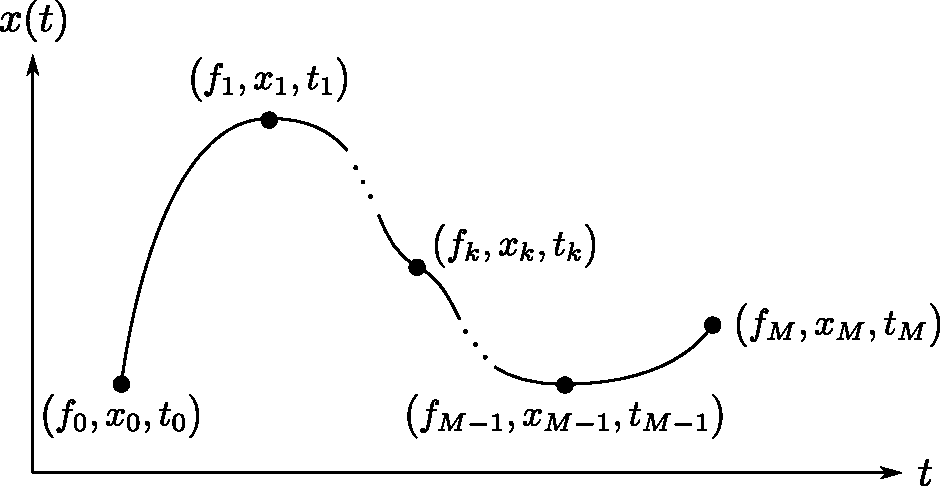
\includegraphics[width=0.8\linewidth]{draw/revisao/pdf/estadoCubico}
	\captionof{figure}[Representação da trajetória do estado considerando uma aproximação de terceiro grau]{Representação da trajetória do estado $ x(t) $ considerando uma aproximação de terceiro grau.}
	\label{fig:revisao:estadoCubico}
	\vspace{\onelineskip}
\end{minipage}

Para fins de aplicação, considere apenas a variável de estado $ x(t) $. Esta pode ser aproximada como segue:
%
\begin{equation}
	\label{eq:revisao:xTrapInterp}
	x(t) = 
	\begin{cases} 
		a_1 \, t^3 + b_1 \, t^2 + c_1 \, t + d_1, & \mbox{se } t_0 \leq t \leq t_1 \\ 
		a_2 \, t^3 + b_2 \, t^2 + c_2 \, t + d_2, & \mbox{se } t_1 < t \leq t_1 \\ 
		\hspace{2cm} \vdots \\
		a_k \, t^3 + b_k \, t^2 + c_k \, t + d_k, & \mbox{se } t_{k-1} < t \leq t_{k} \\ 
		\hspace{2cm} \vdots \\
		a_M \, t^3 + b_M \, t^2 + c_M \, t + d_M, & \mbox{se } t_{M-1} < t \leq t_M
	\end{cases}
\end{equation} 
%
enquanto a derivada de $ x(t) $ (denotada por $ f(t) $) é definida da seguinte forma:
%
\begin{equation}
	\label{eq:revisao:fTrapInterp}
	f(t) = 
	\begin{cases} 
		3 \, a_1 \, t^2 + 2 \, b_1 \, t + c_1, & \mbox{se } t_0 \leq t \leq t_1 \\ 
		3 \, a_2 \, t^2 + 2 \, b_2 \, t + c_2, & \mbox{se } t_1 < t \leq t_2 \\ 
		\hspace{2cm} \vdots \\
		3 \, a_k \, t^2 + 2 \, b_k \, t + c_k, & \mbox{se } t_{k-1} < t \leq t_{k} \\ 
		\hspace{2cm} \vdots \\
		3 \, a_M \, t^2 + 2 \, b_M \, t + c_M, & \mbox{se } t_{M-1} < t \leq t_M
	\end{cases}
\end{equation} 

Verifica-se que a $ k $-ésima \textit{spline} tem como extremos os pontos $ (t_{k-1}, x_{k-1}) $ e $ (t_k, x_k) $ e que as derivadas de $ x(t) $ nesses pontos são dadas por $ f_{k-1} $ e $ f_k $ respectivamente. Logo, os coeficientes $ a_k $, $ b_k $, $ c_k $ e $ d_k $ devem satisfazer \eqref{eq:revisao:splineCubicaEqs}.
%
\begin{equation}
	\label{eq:revisao:splineCubicaEqs}
	\begin{gathered}
		a_k \, t_{k-1}^3 + b_k \, t_{k-1}^2 + c_k \, t_{k-1} + d_k = x_{k-1} \\
		a_k \, t_{k}^3 + b_k \, t_{k}^2 + c_k \, t_{k} + d_k = x_{k} \\
		3 \, a_k \, t_{k-1}^2 + 2 \, b_k \, t_{k-1} + c_k = f_{k-1} \\
		3 \, a_k \, t_{k}^2 + 2 \, b_k \, t_{k} + c_k = f_{k}
	\end{gathered}
\end{equation}

Nota-se que cada \textit{spline} está associada a quatro equações, de forma que um sistema com $ 4M $ equações pode ser construído para que os coeficientes $ a_k $, $ b_k $, $ c_k $ e $ d_k $ sejam determinados para $ k = 1, \, 2, \, \dots, \, M $. 

Considerando, por exemplo, que $ M = 3 $, tem-se as expressões para o estado (ver a Figura \ref{fig:revisao:estadoCubico4Pontos}):
%
\begin{equation}
	\begin{gathered}
		x(t) = 
		\begin{cases} 
			a_1 \, t^3 + b_1 \, t^2 + c_1 \, t + d_1, & \mbox{se } t_0 \leq t \leq t_1 \\
			a_2 \, t^3 + b_2 \, t^2 + c_2 \, t + d_2, & \mbox{se } t_1 < t \leq t_2 \\
			a_3 \, t^3 + b_3 \, t^2 + c_3 \, t + d_3, & \mbox{se } t_2 < t \leq t_3 
		\end{cases}
	\end{gathered}
\end{equation} 
%
e, consequentemente, a sua derivada:
%
\begin{equation}
	f(t) = 
	\begin{cases}
		3 \, a_1 \, t^2 + 2 \, b_1 \, t + c_1, & \mbox{se } t_0 \leq t \leq t_1 \\ 
		3 \, a_2 \, t^2 + 2 \, b_2 \, t + c_2, & \mbox{se } t_1 < t \leq t_2 \\ 
		3 \, a_3 \, t^2 + 2 \, b_3 \, t + c_3, & \mbox{se } t_2 < t \leq t_3 \\ 
	\end{cases}
\end{equation}

\noindent	
\begin{minipage}{\textwidth}
	\vspace{\onelineskip}
	\centering
	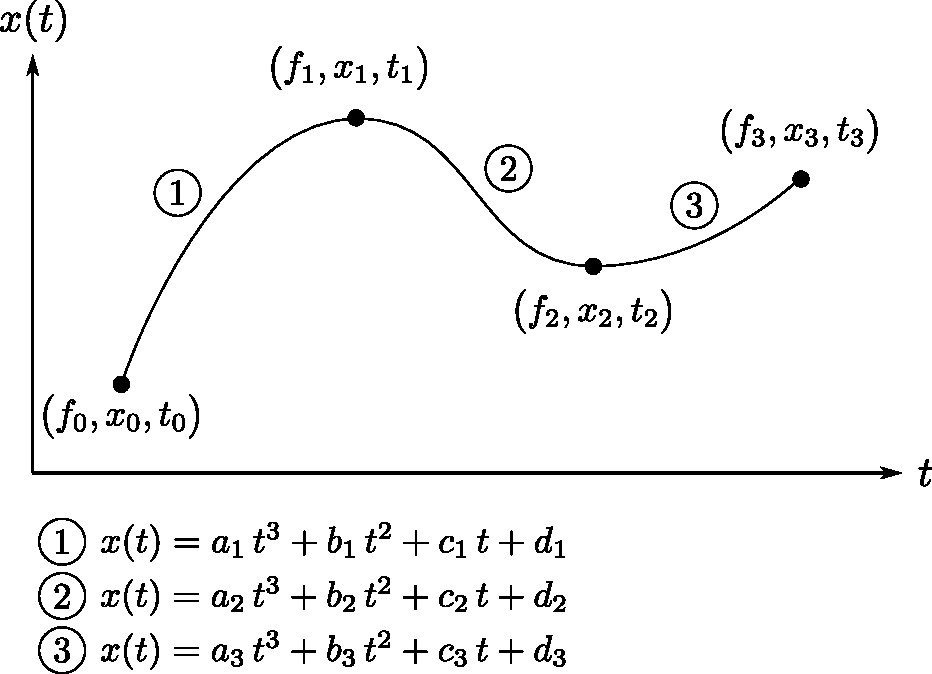
\includegraphics[width=0.8\linewidth]{draw/revisao/pdf/estadoCubico4pontos}
	\captionof{figure}[Representação da trajetória do estado considerando quatro nós de colocação]{Representação da trajetória do estado $ x(t) $ considerando $ M = 3 $.}
	\label{fig:revisao:estadoCubico4Pontos}
	\vspace{\onelineskip}
\end{minipage}

Uma vez que as extremidades de cada \textit{spline}, assim como as derivadas de $ x(t) $ associadas às mesmas, se encontram definidas, é possível que os coeficientes $ a_k $, $ b_k $, $ c_k $, e $ d_k $ sejam determinados por meio da resolução do seguinte sistema de equações:
%
\begin{equation}
\label{eq:revisao:splinesCubicas}
\begin{cases}
x_0 = a_1 \, t_0^3 + b_1 \, t_0^2 + c_1 \, t_0 + d_1 \\
x_1 = a_1 \, t_1^3 + b_1 \, t_1^2 + c_1 \, t_1 + d_1 \\
x_1 = a_2 \, t_1^3 + b_2 \, t_1^2 + c_2 \, t_1 + d_2 \\
x_2 = a_2 \, t_2^3 + b_2 \, t_2^2 + c_2 \, t_2 + d_2 \\
x_2 = a_3 \, t_2^3 + b_3 \, t_2^2 + c_3 \, t_2 + d_3 \\
x_3 = a_3 \, t_3^3 + b_3 \, t_3^2 + c_3 \, t_3 + d_3 \vspace{0.25cm} \\ 
f_0 = 3 \, a_1 \, t_0^2 + 2 \, b_1 \, t_0 + c_1 \\
f_1 = 3 \, a_1 \, t_1^2 + 2 \, b_1 \, t_1 + c_1 \\
f_1 = 3 \, a_2 \, t_1^2 + 2 \, b_2 \, t_1 + c_2 \\
f_2 = 3 \, a_2 \, t_2^2 + 2 \, b_2 \, t_2 + c_2 \\
f_2 = 3 \, a_3 \, t_2^2 + 2 \, b_3 \, t_2 + c_3 \\
f_3 = 3 \, a_3 \, t_3^2 + 2 \, b_3 \, t_3 + c_3
\end{cases}
\end{equation}

Finalmente, é importante enfatizar que, se o problema em questão for composto por um vetor de variáveis de estado e por um vetor de variáveis de controle, a metodologia apresentada por ser facilmente estendida para essa finalidade.

%Caso $ \mathbf{x}^T(t) = \begin{bmatrix} x^{(1)}(t) & \dots & x^{(n)}(t) \end{bmatrix} $ de forma que vários perfis de estado devam ser determinados, basta que o procedimento apresentado seja aplicado a cada perfil. Além disso, se $ M $ for maior do que 3, apenas verifica-se o crescimento do sistema \eqref{eq:revisao:splinesCubicas}. Uma função desenvolvida pelo autor para implementação da interpolação cúbica dos estados, intitulada \texttt{spline3()}, pode ser acessada em \url{https://cutt.ly/ijU0S2Q}.

\subsection{Colocação Hermite-Simpson}
\label{sec:revisao:hersim}

\todo[inline, color=pink]{Colocação Hermite-Simpson}

A colocação Hermite-Simpson é baseada na quadratura de Simpson, empregada tanto na computação do integrando $ L$ associado à função objetivo, quanto na discretização das restrições dinâmicas. Para que a quadratura de Simpson seja implementada é necessário que nós de colocação intermediários, posicionados entre os nós de colocação originais, sejam definidos \cite{kelly_introduction_2017}. As grandezas associadas aos nós intermediários são representadas utilizando-se uma barra. Por exemplo, os valores assumidos pelos controles nos nós intermediários são denotados por $ \mathbf{\overline{u}}_k, \; k = 0, \, 2, \, \dots, \, M-1 $. 

Mais especificamente, o valor atribuído aos controles $ u(t) $ no nó de colocação intermediário posicionado entre os nós $ k $ e $ k+1 $ é denotado por $ \overline{u}_k $. Assumindo-se $ h_k = t_{k+1} - t_k $, determina-se a integral de $L$ de acordo com a seguinte equação:
%
\begin{equation}
\label{eq:revisao:hersim:integral}
\int_{t_0}^{t_f} L \big( \mathbf{x}(t), \mathbf{u}(t), t \big) \, dt \approx \sum_{k=0}^{M-1} \frac{1}{6} h_k (L_k + 4 \, \overline{L}_{k} + L_{k+1})
\end{equation}
%
sendo $ L_k =  L \big( \mathbf{x}_k, \mathbf{u}_k, t_k \big) $ e $ \overline{L}_{k} =  L \big( \mathbf{\overline{x}}_{k}, \mathbf{\overline{u}}_{k}, \overline{t}_{k} \big)$ \cite{kelly_introduction_2017}. 

Enquanto $ \mathbf{\overline{x}}_{k} $ pode ser computado a partir dos valores atribuídos a $ \mathbf{x}_{k} $ e $ \mathbf{x}_{k+1} $, como será mostrado adiante, e $ \overline{t}_{k} = \dfrac{t_{k} + t_{k+1}}{2} $, $ \mathbf{\overline{u}}_{k} $ deve ser uma variável de projeto assim como $ \mathbf{u}_{k} $ e $ \mathbf{x}_{k} $ \cite{kelly_introduction_2017}. Nota-se, portanto, que o PPNL formulado com base na colocação Hermite-Simpson possui mais variáveis de projeto que aquele obtido por meio da colocação trapezoidal, considerando-se que o mesmo número de nós de colocação seja utilizado em ambos os casos. 

Após a discretização do vetor de variáveis de estados é possível que as restrições diferenciais associadas à dinâmica do PCO sejam representadas por um conjunto de restrições algébricas. Para tanto, é necessário que as restrições dinâmicas sejam reescritas na forma integral e que a quadratura de Simpson seja empregada \cite{kelly_introduction_2017}:
%
\begin{subequations}
\begin{equation}
\label{eq:revisao:hersim:restricaoDinamica}
\dot{\mathbf{x}}(t) = \mathbf{f}(\mathbf{x}(t), \mathbf{u}(t), t)
\end{equation}
\vspace{-0.5cm}
\begin{equation}
\int_{t_k}^{t_{k+1}} \dot{\mathbf{x}}(t) \, dt = \int_{t_k}^{t_{k+1}} \mathbf{f}(\mathbf{x}(t), \mathbf{u}(t), t) \, dt
\end{equation}
\vspace{-0.15cm}
\begin{equation}
\mathbf{x}_{k+1} - \mathbf{x}_k \approx \frac{1}{6} h_k (\mathbf{f}_{k} + 4 \, \mathbf{\overline{f}}_{k} + \mathbf{f}_{k+1})
\end{equation}
\end{subequations}

Assim sendo, $ M $ restrições de igualdade algébricas são formuladas com base na aproximação descrita anteriormente, isto é:
%
\begin{equation}
\mathbf{x}_{k+1} - \mathbf{x}_k - \frac{1}{6} h_k (\mathbf{f}_{k} + 4 \, \mathbf{\overline{f}}_{k} + \mathbf{f}_{k+1}) = \mathbf{0}, \hspace{0.25cm} k = 0, \, \dots, \, M-1
\end{equation}
%
sendo $ \mathbf{f}_k = \mathbf{f}(\mathbf{x}_k, \mathbf{u}_k, t_k) $ e $ \mathbf{\overline{f}}_{k} = \mathbf{f}(\mathbf{\overline{x}}_{k}, \mathbf{\overline{u}}_{k}, \overline{t}_{k}) $ obtidos a partir da computação da dinâmica do sistema.  

Para que $ \mathbf{\overline{f}}_{k} $ possa ser computado é necessário antes que $ \mathbf{\overline{x}}_{k} $ seja determinado empregando-se a interpolação de Hermite:
%
\begin{equation}
	\label{eq:revisao:interpHermite}
	\overline{\mathbf{x}}_{k} = \frac{1}{2} (\mathbf{x}_{k} + \mathbf{x}_{k+1}) + \frac{h_k}{8} (\mathbf{f}_{k} - \mathbf{f}_{k+1}) 
\end{equation}

Assim sendo é possível que $ \mathbf{\overline{x}}_{k} $ seja computado segundo  \eqref{eq:revisao:interpHermite}, ou que $ \mathbf{\overline{x}}_{k} $ seja considerado uma variável de projeto. Nesse último caso, é necessário que outras $ M $ restrições de igualdade algébricas, definidas a partir de \eqref{eq:revisao:interpHermite}, sejam acrescentadas ao PPNL: 
%
\begin{equation}
\mathbf{\overline{x}}_{k} - \frac{1}{2} (\mathbf{x}_{k} + \mathbf{x}_{k+1}) - \frac{h_k}{8} (\mathbf{f}_{k} - \mathbf{f}_{k+1}) = \mathbf{0}, \hspace{0.25cm} k = 0, \, \dots, \, M-1
\end{equation}

Analogamente ao que foi desenvolvido para a regra trapezoidal, as restrições associadas ao PCO podem ser transcritas da seguinte forma: 
%
\begin{subequations}
\begin{equation}
		\mathbf{x_L} \leq \mathbf{x}(t) \leq \mathbf{x_U} \rightarrow 
		\begin{cases}
			\mathbf{x_L} \leq \mathbf{x}_k \leq \mathbf{x_U}, \; k = 0, \, \dots, \, M  \\
			\mathbf{x_L} \leq \mathbf{\overline{x}}_{k} \leq \mathbf{x_U}, \; k = 0, \, \dots, \, M-1
		\end{cases} 
\end{equation}
\vspace{-0.1cm}
\begin{equation}
		\mathbf{u_L} \leq \mathbf{u}(t) \leq \mathbf{u_U} \rightarrow 
		\begin{cases}
			\mathbf{u_L} \leq \mathbf{u}_k \leq \mathbf{u_U}, \; k = 0, \, \dots, \, M \\
			\mathbf{u_L} \leq \mathbf{\overline{u}}_{k} \leq \mathbf{u_U}, \; k = 0, \, \dots, \, M-1
		\end{cases}
\end{equation}
\vspace{0.025cm}
\begin{equation}
	\mathbf{c}(\mathbf{x}(t), \mathbf{u}(t), t) \leq \mathbf{0} \rightarrow 
		\begin{cases}
			\mathbf{c}(\mathbf{x}_k, \mathbf{u}_k, t_k) \leq \mathbf{0}, \; k = 0, \, \dots, \, M \\
			\mathbf{c}(\mathbf{\overline{x}}_{k}, \mathbf{\overline{u}}_{k}, \overline{t}_{k}) \leq \mathbf{0}, \; k = 0, \, \dots, \, M-1
		\end{cases} 
\end{equation}
\vspace{-0.15cm}
\begin{equation}
{\bm \psi}(\mathbf{x}(t_f), t_f) \leq \mathbf{0}  \rightarrow {\bm \psi}(\mathbf{x}_M, t_M) \leq \mathbf{0} 
\end{equation}
\end{subequations}
%
em que a condição inicial é dada como:
%
\begin{equation}
\mathbf{x}_k = \mathbf{x_0}, \hspace{0.25cm} k = 0 
\end{equation}
%

%As variáveis de projeto associadas ao PPNL advindo do processo de transcrição, considerando-se o caso geral em que $ t_0 $ e $ t_f $ devem ser determinados assim como $ \mathbf{u}_k $ e $ \mathbf{x}_k $, são introduzidas em \eqref{eq:revisao:variaveisPPNLHersim}
%%
%\begin{equation}
%\label{eq:revisao:variaveisPPNLHersim}
%\mathbf{z}^T = \begin{bmatrix} \mathbf{z_t}^T & \mathbf{z_x}^T & \mathbf{z_u}^T & \mathbf{z_{u+\frac{1}{2}}}^T \end{bmatrix} 
%\end{equation}
%% 
%em que
%%
%\begin{equation}
%\begin{gathered}
%\mathbf{z_t}^T = \begin{bmatrix} t_0 & t_f \end{bmatrix} \\
%\mathbf{z_x}^T = \begin{bmatrix} x^{(1)}_0 & x^{(1)}_1 & \dots & x^{(1)}_M & \dots & x^{(n)}_0 & x^{(n)}_1 & \dots & x^{(n)}_M \end{bmatrix} \\
%\mathbf{z_u}^T = \begin{bmatrix} u^{(1)}_0 & u^{(1)}_1 & \dots & u^{(1)}_M & \dots & u^{(n)}_0 & u^{(n)}_1 & \dots & u^{(n)}_M \end{bmatrix} \\
%\mathbf{z_{u+\frac{1}{2}}}^T = \begin{bmatrix} u^{(1)}_{\frac{1}{2}} & u^{(1)}_{1+\frac{1}{2}} & \dots & u^{(1)}_{M-1+\frac{1}{2}} & \dots & u^{(n)}_{\frac{1}{2}} & u^{(n)}_{1+\frac{1}{2}} & \dots & u^{(n)}_{M-1+\frac{1}{2}} \end{bmatrix} 
%\end{gathered}
%\end{equation}
%
%e assumindo-se que a interpolação de Hermite seja empregada na computação de $ \mathbf{\overline{x}}_{k} $.

Para a colocação Hermite-Simpson, o PCO é dado como:
%
\begin{subequations}
\begin{equation}
	\underset{\mathbf{\overline{u}}_k, \, \mathbf{u}_k, \, \mathbf{x}_k}{\text{min}} \; J = \varphi \big( \mathbf{x}_M, t_M \big) + \sum_{k=0}^{M-1} \frac{1}{6} h_k (L_k + 4 \, \overline{L}_{k} + L_{k+1})
\end{equation}
\vspace{-0.1cm}
\begin{equation}
	\mathbf{x}_{k+1} - \mathbf{x}_k - \frac{1}{6} h_k (\mathbf{f}_{k} + 4 \, \mathbf{\overline{f}}_{k} + \mathbf{f}_{k+1}) = \mathbf{0}, \hspace{1cm} k = 0, \, \dots, \, M-1
\end{equation}
\vspace{-0.75cm}
\begin{equation}
	\mathbf{x}(t_0) = \mathbf{x_0}
\end{equation}
\vspace{-0.75cm}
\begin{equation}
\mathbf{x_L} \leq \mathbf{x}_k \leq \mathbf{x_U}, \hspace{0.25cm} k = 0, \, \dots, \, M 
\end{equation}
\vspace{-0.75cm}
\begin{equation}
\mathbf{x_L} \leq \mathbf{\overline{x}}_k \leq \mathbf{x_U}, \hspace{0.25cm} k = 0, \, \dots, \, M-1
\end{equation}
\vspace{-0.75cm}
\begin{equation}
\mathbf{u_L} \leq \mathbf{u}_k \leq \mathbf{u_U}, \hspace{0.25cm} k = 0, \, \dots, \, M 
\end{equation}
\vspace{-0.75cm}
\begin{equation}
\mathbf{u_L} \leq \mathbf{\overline{u}}_k \leq \mathbf{u_U} \hspace{0.25cm} k = 0, \, \dots, \, M-1 
\end{equation}
\vspace{-0.75cm}
\begin{equation}
\mathbf{c}(\mathbf{x}_k, \mathbf{u}_k, t_k) \leq \mathbf{0}, \hspace{0.25cm} k = 0, \, \dots, \, M 
\end{equation}
\vspace{-0.75cm}
\begin{equation}
\mathbf{c}(\mathbf{\overline{x}}_k, \mathbf{\overline{u}}_k, \overline{t}_k) \leq \mathbf{0}, \hspace{0.25cm} k = 0, \, \dots, \, M-1 
\end{equation}
\vspace{-0.75cm}
\begin{equation}
{\bm \psi}(\mathbf{x}_M, t_M) \leq \mathbf{0} 
\end{equation}
\end{subequations}
%
para $ t_0 $ e $ t_f $ conhecidos. Não sendo esse o caso, devem-se adotar $ t_0 $ e $ t_f $ como variáveis de projeto, e as restrições:
%
\begin{subequations}
\begin{equation}
t_{0L} \leq t_0 \leq t_{0U}
\end{equation}
\vspace{-0.75cm}
\begin{equation}
t_{fL} \leq t_f \leq t_{fU}
\end{equation} 
\end{subequations}
%
em que $ t_{0L} $ e $ t_{fL} $ representam os limites inferiores e $ t_{0U} $ e $ t_{fU} $ os limites superiores. 

Uma vez que o PPNL tenha sido resolvido e que tanto $ \mathbf{x}_k $ quanto $ \mathbf{u}_k $ tenham sido determinados para $ k = 0, \, 1, \, \dots, \, M $, é possível que as trajetórias de estados e controles sejam obtidas. A colocação Hermite-Simpson é baseada na suposição de que os perfis de controle evoluem quadraticamente entre os nós de colocação e que podem, portanto, ser aproximados pela concatenação de polinômios (ou \textit{splines}) de segunda ordem, conforme ilustrado na Figura \ref{fig:revisao:controleQuadratico} \cite{kelly_introduction_2017}. 

\noindent	
\begin{minipage}{\textwidth}
	\vspace{\onelineskip}
	\centering
	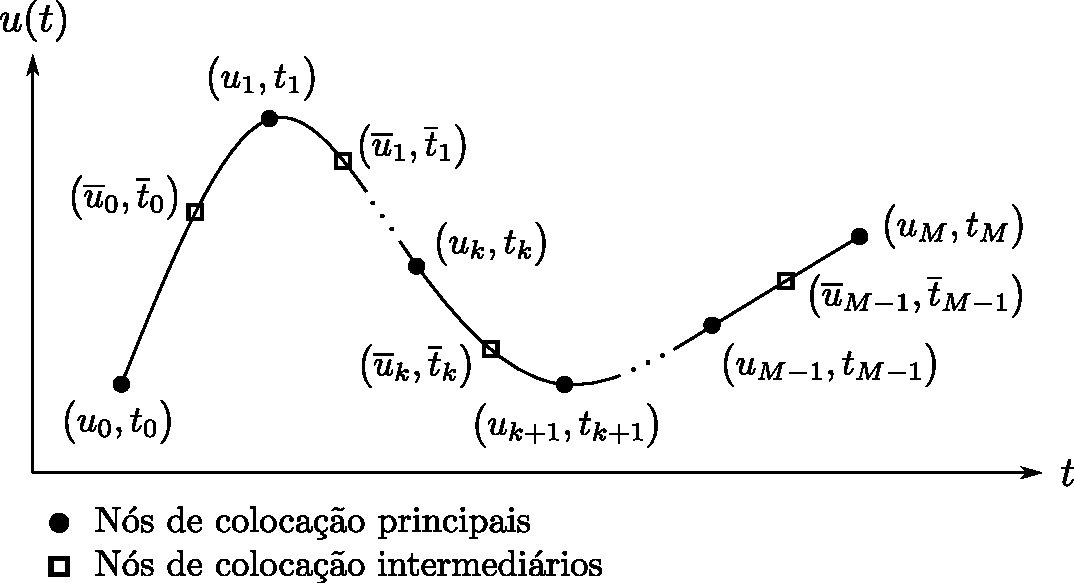
\includegraphics[width=0.9\linewidth]{draw/revisao/pdf/controleQuadratico}
	\captionof{figure}[Representação da trajetória do controle considerando aproximações quadráticas]{Representação da trajetória do controle $ u(t) $ considerando aproximações quadráticas.}
	\label{fig:revisao:controleQuadratico}
	\vspace{\onelineskip}
\end{minipage}

Supondo que exista apenas um controle $u(t)$, pode-se determinar o mesmo conforme a seguinte relação.
%
\begin{equation}
\label{eq:revisao:uHersimInterp}
u(t) = 
\begin{cases} 
a_1 \, t^2 + b_1 \, t + c_1, & \mbox{se } t_0 \leq t \leq t_1 \\ 
a_2 \, t^2 + b_2 \, t + c_2, & \mbox{se } t_1 \leq t \leq t_2 \\ 
\hspace{1.25cm} \vdots \\
a_k \, t^2 + b_k \, t + c_k, & \mbox{se } t_{k-1} \leq t \leq t_k \\ 
\hspace{1.25cm} \vdots \\
a_M \, t^2 + b_M \, t + c_M, & \mbox{se } t_{M-1} \leq t \leq t_{M} 
\end{cases}
\end{equation} 

Nesta equação observa-se que a $ k $-ésima \textit{spline} tem como extremos os pontos $ (t_{k-1}, u_{k-1}) $ e $ (t_k, u_k) $, e como ponto médio $ (\overline{t}_{k-1}, \overline{u}_{k-1}) $. Logo, os coeficientes $ a_k $, $ b_k $ e $ c_k $ devem satisfazer a seguinte relação:
%
\begin{subequations}
\begin{equation}
\label{eq:revisao:splineHermite}
a_k \, t_{k-1}^2 + b_k \, t_{k-1} + c_k = u_{k-1}
\end{equation}
\vspace{-0.75cm}
\begin{equation}
a_k \, \overline{t}_{k-1}^2 + b_k \, \overline{t}_{k-1} + c_k = \overline{u}_{k-1} \end{equation}
\vspace{-0.75cm}
\begin{equation}
a_k \, t_{k}^2 + b_k \, t_{k} + c_k = u_{k} 
\end{equation}
\end{subequations}

Nota-se que a cada \textit{spline} estão associadas três equações, de forma que um sistema com $ 3M $ equações pode ser construído para que os coeficientes $ a_k $, $ b_k $ e $ c_k $ sejam determinados para $ k = 1, \, 2, \, \dots, \, M $. 

Para $ M = 3 $, tem-se a seguinte estratégia de controle (ver a Figura \ref{fig:revisao:controleQuadratico4pontos}):
%
\begin{equation}
u(t) = 
\begin{cases} 
a_1 \, t^2 + b_1 \, t + c_1, & \mbox{se } t_0 \leq t \leq t_1 \\ 
a_2 \, t^2 + b_2 \, t + c_2, & \mbox{se } t_1 < t \leq t_2 \\ 
a_3 \, t^2 + b_3 \, t + c_3, & \mbox{se } t_2 < t \leq t_3 
\end{cases}
\end{equation} 

\noindent	
\begin{minipage}{\textwidth}
	\vspace{\onelineskip}
	\centering
	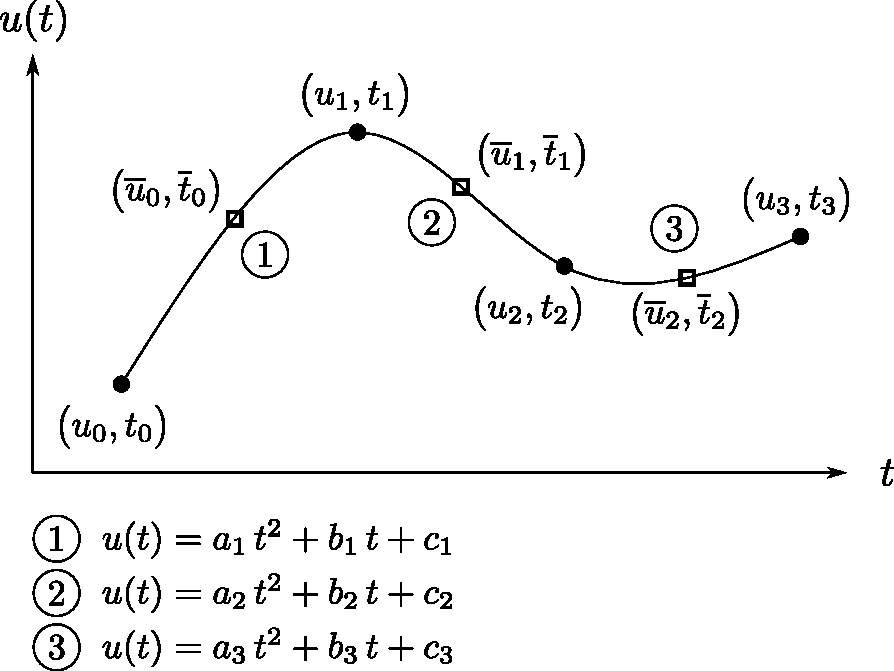
\includegraphics[width=0.75\linewidth]{draw/revisao/pdf/controleQuadratico4pontos}
	\captionof{figure}[Representação da trajetória do controle considerando quatro nós de colocação]{Representação da trajetória do controle $ u(t) $ considerando $ M = 3 $.}
	\label{fig:revisao:controleQuadratico4pontos}
	\vspace{\onelineskip}
\end{minipage}

Neste caso, é possível determinar  os coeficientes $ a_k $, $ b_k $ e $ c_k $ via solução do seguinte sistema de equações:
%
\begin{equation}
\label{eq:revisao:splinesQuadraticas}
\begin{cases}
u_0 = a_1 \, t_0^2 + b_1 \, t_0 + c_1 \\
u_1 = a_1 \, t_1^2 + b_1 \, t_1 + c_1 \\
u_1 = a_2 \, t_1^2 + b_2 \, t_1 + c_2 \\
u_2 = a_2 \, t_2^2 + b_2 \, t_2 + c_2 \\
u_2 = a_3 \, t_2^2 + b_3 \, t_2 + c_3 \\
u_3 = a_3 \, t_3^2 + b_3 \, t_3 + c_3 \vspace{0.25cm} \\ 
\overline{u}_0 = a_1 \, \overline{t}_0^2 + b_1 \, \overline{t}_0 + c_1 \\
\overline{u}_1 = a_2 \, \overline{t}_1^2 + b_2 \, \overline{t}_0 + c_2 \\
\overline{u}_2 = a_3 \, \overline{t}_2^2 + b_3 \, \overline{t}_0 + c_3
\end{cases}
\end{equation}

É importante ressaltar que o procedimento apresentado pode ser facilmente adaptado para um vetor de variáveis de controle. A trajetória dos estados entre os nós de colocação, por sua vez, é aproximada utilizando-se \textit{splines} cúbicas, conforme appresentado anteriormente na  Seção \ref{sec:revisao:trap}. 

%Caso $ \mathbf{u}^T(t) = \begin{bmatrix} x^{(1)}(t) & \dots & x^{(n)}(t) \end{bmatrix} $ de forma que vários perfis de controle devam ser determinados, basta que o procedimento apresentado seja aplicado a cada perfil. Além disso, se $ M $ for maior do que 3, apenas verifica-se o crescimento do sistema \eqref{eq:revisao:splinesLineares}. Uma função desenvolvida pelo autor para implementação da interpolação quadrática dos controles, intitulada \texttt{spline2()}, pode ser acessada em \url{https://cutt.ly/ijU0S2Q}.

\subsection{Colocação pseudo-espectral}

\todo[inline, color=pink]{Colocação pseudo-espectral}

Os métodos pseudo-espectrais foram inicialmente propostos para solução de equações diferenciais, com grande aplicabilidade em fluidodinâmica computacional. Desde 1995, esses métodos vem sendo empregados na solução de PCOs. Diferentemente dos métodos baseados em diferenças finitas, que fazem uso de informações locais, os métodos pseudo-espectrais utilizam amostras de todo o domínio na determinação dos valores assumidos pela derivada de uma dada função \cite{becerra_tutorial_2010}.

A colocação pseudo-espectral baseia-se na aproximação do vetor de variáveis de estado e de controle por uma somatória de polinômios suaves, como os de Legendre ou Chebyshev, no intervalo $ [ -1, \, 1 ] $. Nesse caso, cada estado associado a $ \mathbf{x}(t) $ é aproximado por um único polinômio de alta ordem, assim como cada controle associado a $ \mathbf{u}(t) $ \cite{becerra_psopt_2019}. Vale ressaltar que essa abordagem é distinta daquelas nas quais se baseiam os métodos apresentados nas Seções \ref{sec:revisao:trap} e \ref{sec:revisao:hersim}, em que os estados e controles são aproximados por uma concatenação de vários polinômios de baixa ordem. 
Os métodos pseudo-espectrais apresentam taxa de convergência exponencial, o que possibilita a obtenção de resultados bastante satisfatórios mesmo quando utilizam-se malhas grosseiras. Além disso, esses métodos viabilizam a computação de derivadas e integrais de forma simples, direta, e precisa, o que pode ser bastante útil na resolução de PCOs, cuja formulação depende diretamente dessas operações \cite{becerra_tutorial_2010}. 

Os resultados advindos do emprego da colocação pseudo-espectral apresentados no presente trabalho foram obtidos com base na utilização dos polinômios de Legendre. Um polinômio de Legendre de ordem $ M $ pode ser computado segundo a seguinte relação:
%
\begin{equation}
	\label{eq:revisao:legendre}
	L_M(\tau)  = \frac{1}{2^M M!} \frac{d^M}{d \tau^M}(\tau^2 - 1)^M
\end{equation}

Alguns exemplos de polinômios de Legendre são descritos a seguir:
%
\begin{equation}
	\label{eq:revisao:ExLegendre}
	\begin{gathered}
		L_0(\tau) = 1 \\
		L_1(\tau) = \tau \\
		L_2(\tau) = \frac{1}{2} (3 \tau^2 - 1) \\
		L_3(\tau) = \frac{1}{2} (5 \tau^3 - 3\tau)
	\end{gathered}
\end{equation}

Os nós de colocação associados à essa abordagem devem ser distribuídos de acordo com os nós de Legendre-Gauss-Lobato (LGL): 
%
\begin{equation}
{\bm \tau_\mathbf{LGL}} = \begin{bmatrix} \tau_0 & \dots & \tau_k & \dots & \tau_M \end{bmatrix}
\end{equation}
%

Estes são definidos de forma que $ \tau_0 = -1$, $ \tau_M = 1 $, e $ \tau_k $, para $ k = 1, \dots, M-1 $, são as raízes do polinômio $ \dfrac{dL_M(\tau)}{d\tau} $ \cite{becerra_tutorial_2010}.

Se, por exemplo, $ M = 5 $, tem-se:
%
\begin{equation}
	L_5(\tau) = \frac{63}{8} \tau^5 - \frac{35}{4} \tau^3 + \frac{15}{8} \tau 
\end{equation}
% 
sendo que a respectiva derivada é dada como:
%
\begin{equation}
	\label{eq:revisao:dL5}
	\frac{dL_5(\tau)}{d\tau} = \frac{315}{8} \tau^4 - \frac{105}{4} \tau^2 + \frac{15}{8}  
\end{equation}

As raízes dessa última equação são iguais a $ \pm 0,7651 $ e $ \pm 0,2852 $, respectivamente. Assim sendo, os nós $ LGL $ para $ M = 5 $ (ver a Figura \ref{fig:revisao:nosLGL}) são dados por:
%
\begin{equation}
	\label{eq:revisao:nosLGL5}
	{\bm \tau_\mathbf{LGL}} = \begin{bmatrix} -1 & -0,7651 & -0,2851 & 0,2852 & 0,7651 & 1 \end{bmatrix} 
\end{equation}

\noindent	
\begin{minipage}{\textwidth}
	\vspace{\onelineskip}
	\centering
	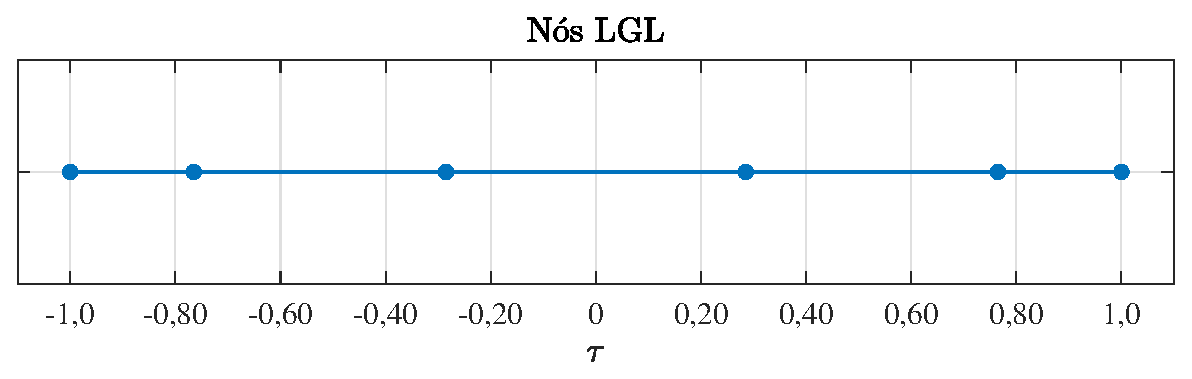
\includegraphics[width=1\linewidth]{fig/revisao/nosLGL}
	\captionof{figure}[Representação dos nós LGL]{Nós LGL para $ M = 5 $.}
	\label{fig:revisao:nosLGL}
	\vspace{\onelineskip}
\end{minipage}

Cabe ressaltar que a adoção do nós LGL possibilita que os estados e controles sejam aproximados com maior precisão e que as operações de derivação e integração associadas a essas variáveis sejam computadas de forma mais acurada. Se outro tipo de polinômio fosse empregado na interpolação dos estados e controles, como por exemplo o polinômio de Chebyshev, uma metodologia distinta seria adotada na determinação dos nós de colocação \cite{becerra_tutorial_2010}.

Como dito anteriormente, os estados e controles são aproximados pelo somatório de polinômios de Legendre no intervalo $ \tau \in [-1, \, 1] $. Além disso, é nesse mesmo intervalo que os nós LGL são definidos. No entanto, tanto os estados quanto os controles devem assumir valores em $ t \in [t_0, \, t_f] $. Assim sendo, conclui-se que a implementação da colocação pseudo-espectral depende da mudança de domínio descrito pela seguinte relação \cite{becerra_tutorial_2010}:
%
\begin{equation}
	\label{eq:revisao:mudancaDominioPseudoEspectral}
	\tau \leftarrow \frac{2}{t_f - t_0} t - \frac{t_f + t_0}{t_f - t_0}
\end{equation}
%

Neste caso, o PCO considerando esta abordagem pode ser formulado como segue \cite{becerra_psopt_2019}:
%
\begin{subequations}
\begin{equation}
\label{eq:revisao:PCOPseudoEspectral}
\underset{\mathbf{u}(\tau)}{\text{min}} \; J = \varphi \big( \mathbf{x}(1), 1 \big) + \frac{t_f - t_0}{2} \int_{-1}^{1} L \big( \mathbf{x}(\tau), \mathbf{u}(\tau), \tau \big) \, d\tau
\end{equation}
\vspace{-0.2cm}
\begin{equation}
\mathbf{\dot{x}}(\tau) = \frac{t_f - t_0}{2} \, \mathbf{f} \big( \mathbf{x}(\tau), \mathbf{u}(\tau), \tau \big), \; \mathbf{x}(-1) = \mathbf{x_0}
\end{equation}
\vspace{-0.7cm}
\begin{equation}
\mathbf{x_L} \leq \mathbf{x}(\tau) \leq \mathbf{x_U}
\end{equation}
\vspace{-0.7cm}
\begin{equation}
\mathbf{u_L} \leq \mathbf{u}(\tau) \leq \mathbf{u_U}
\end{equation}
\vspace{-0.7cm}
\begin{equation}
\mathbf{c}(\mathbf{x}(\tau), \mathbf{u}(\tau), \tau) \leq \mathbf{0}
\end{equation}
\vspace{-0.7cm}
\begin{equation}
{\bm \psi}(\mathbf{x}(1), 1) \leq \mathbf{0} 
\end{equation}
\end{subequations}

Então, para que a colocação pseudo-espectral de Legendre seja implementada, cada estado $ x(t) $ associado a $ \mathbf{x}(t) $ e cada controle $ u(t) $ associado a $ \mathbf{u}(t) $ devem ser aproximados segundo as seguintes relações:
%
\begin{subequations}
\begin{equation}
\label{eq:revisao:pseudoEspectral:estadosControles}
x(\tau) \approx \sum_{k = 0}^{M} x(\tau_k) \phi_k(\tau)
\end{equation}
\vspace{-0.15cm}
\begin{equation}
u(\tau) \approx \sum_{k = 0}^{M} u(\tau_k) \phi_k(\tau) 
\end{equation}
\end{subequations}
%
sendo $ \tau_k $ o $ k $-ésimo nó LGL e $ \phi_k(\tau) $ o $ k $-ésimo polinômio interpolador de Lagrange \cite{becerra_tutorial_2010}:
%
\begin{equation}
	\label{eq:revisao:pseudoEspectral:interpoladorLagrange}
	\phi_k(\tau) = \frac{1}{M(M+1) L_M(\tau_k)} \frac{(\tau^2 - 1) \dot{L}_M(\tau)}{\tau - \tau_k}
\end{equation} 

\todo[inline, size=normalsize, color=pink]{Falar de como a integral $ \int L dt $ é aproximada e de como as derivadas dos estados são aproximadas}

A integral de $L$ é computada empregando-se a quadratura de Gauss:
%
\begin{equation}
	\int_{-1}^{1} L \big( \mathbf{x}(\tau), \mathbf{u}(\tau), \tau \big) \, d\tau \approx \sum_{k=0}^{M} L(\tau_k) w_k
\end{equation}
%
sendo $ w_k $ um peso definido como \cite{becerra_tutorial_2010}:
%
\begin{equation}
	w_k = \frac{2}{M(M+1)} \frac{1}{L_N^2(\tau_k)}
\end{equation}

Vale ressaltar que $ L_M $ e $ L $ representam, respectivamente, o polinômio de Legendre de ordem $ M $ e o integrando associado ao termo de Lagrange da função objetivo $ J $. Dada a semelhança entre as notações atribuídas a essas grandezas, é preciso cuidado para que não haja confusões. 

A computação das derivadas dos estados nos nós de colocação é baseada na definição da matriz de diferenciação $ D $: 
%
\begin{equation}
	D_{ki} = \left\{
	\begin{array}{cl}
		\dfrac{L_M(\tau_k)}{(\tau_k - \tau_i)L_M(\tau_i)} & \text{se } k \neq i \vspace{0.25cm} \\
		-\dfrac{M(M+1)}{4} & \text{se } k = i = 0 \vspace{0.25cm}\\
		\dfrac{M(M+1)}{4} & \text{se } k = i = N \vspace{0.25cm} \\
		0 & \text{nos demais casos} 
	\end{array}
	\right.
\end{equation}  
%
e depende dos valores atribuídos aos estados em cada nó de colocação de forma que:
%
\begin{equation}
	\label{eq:revisao:aproximacaoDerivadas}
	\dot{x}(\tau_k) \approx \sum_{i=0}^{M} D_{ki} \, x(\tau_k)
\end{equation}
%

É possível ainda que a relação acima seja reescrita na forma matricial \cite{becerra_tutorial_2010}:
%
\begin{equation}
	\begin{bmatrix}
		\dot{x}(\tau_0) \\
		\dot{x}(\tau_1) \\
		\vdots \\
		\dot{x}(\tau_M) 
	\end{bmatrix} = 
	\begin{bmatrix}
		D_{00} & D_{01} & \cdots & D_{0M} \\
		D_{00} & D_{01} & \cdots & D_{0M} \\
		\cdots & \cdots & \ddots & \vdots \\
		D_{M0} & D_{M1} & \cdots & D_{MM} 
	\end{bmatrix}
	\begin{bmatrix}
		x(\tau_0) \\
		x(\tau_1) \\
		\vdots \\
		x(\tau_M) 
	\end{bmatrix}
\end{equation}

Assim sendo, $ M $ restrições de igualdade algébricas são formuladas como segue:
%
\begin{equation}
\mathbf{\dot{x}}(\tau_k) - \frac{t_f - t_0}{2} \, \mathbf{f} \big( \mathbf{x}(\tau_k), \mathbf{u}(\tau_k), \tau_k \big) = 0, \hspace{0.25cm} k = 0, \, \dots, \, M-1
\end{equation}
%
em que a derivada pode ser computada pela Eq. \eqref{eq:revisao:aproximacaoDerivadas}.

Assim como foi apresentado anteriormente, as restrições laterais, terminais, e de caminho podem ser reescritas como \cite{becerra_psopt_2019}: 
%
\begin{subequations}
\begin{equation}
\mathbf{x_L} \leq \mathbf{x}(t) \leq \mathbf{x_U} \rightarrow \mathbf{x_L} \leq \mathbf{x}(\tau_k) \leq \mathbf{x_U}, \; k = 0, \, \dots, \, M
\end{equation}
\vspace{-0.85cm}
\begin{equation}
\mathbf{u_L} \leq \mathbf{u}(t) \leq \mathbf{u_U} \rightarrow \mathbf{u_L} \leq \mathbf{u}(\tau_k) \leq \mathbf{u_U}, \; k = 0, \, \dots, \, M
\end{equation}
\vspace{-0.75cm}
\begin{equation}
\mathbf{c}(\mathbf{x}(t), \mathbf{u}(t), t) \leq \mathbf{0} \rightarrow \mathbf{c}(\mathbf{x}(\tau_k), \mathbf{u}(\tau_k), \tau_k) \leq \mathbf{0}, \; k = 0, \, \dots, \, M 
\end{equation}
\vspace{-0.75cm}
\begin{equation}
{\bm \psi}(\mathbf{x}(t_f), t_f) \leq \mathbf{0}  \rightarrow {\bm \psi}(\mathbf{x}(1), 1) \leq \mathbf{0} 
\end{equation}
\end{subequations}
%
em que a condição inicial é dada como:
%
\begin{equation}
\mathbf{x}_k = \mathbf{x_0}, \hspace{0.25cm} k = 0 
\end{equation}
%

Em resumo, para esta abordagem, o PCO é descrito como:
%
\begin{subequations}
\begin{equation}
\underset{\mathbf{u}(\tau_k), \, \mathbf{x}(\tau_k)}{\text{min}} \; J = \varphi \big( \mathbf{x}(1), 1 \big) + \frac{t_f - t_0}{2} \sum_{k=0}^{M} L(\tau_k) w_k 
\end{equation}
\vspace{-0.15cm}
\begin{equation}
\mathbf{\dot{x}}(\tau_k) - \frac{t_f - t_0}{2} \, \mathbf{f} \big( \mathbf{x}(\tau_k), \mathbf{u}(\tau_k), \tau_k \big) = 0, \hspace{0.25cm} k = 0, \, \dots, \, M
\end{equation}
\vspace{-0.7cm}
\begin{equation}
\mathbf{x}(-1) = \mathbf{x_0}
\end{equation}
\vspace{-0.7cm}
\begin{equation}
\mathbf{x_L} \leq \mathbf{x}(\tau_k) \leq \mathbf{x_U}, \hspace{0.25cm} k = 0, \, \dots, \, M 
\end{equation}
\vspace{-0.7cm}
\begin{equation}
\mathbf{u_L} \leq \mathbf{u}(\tau_k) \leq \mathbf{u_U}, \hspace{0.25cm} k = 0, \, \dots, \, M 
\end{equation}
\vspace{-0.7cm}
\begin{equation}
\mathbf{c}(\mathbf{x}(\tau_k), \mathbf{u}(\tau_k), \tau_k) \leq \mathbf{0}, \hspace{0.25cm} k = 0, \, \dots, \, M
\end{equation}
\vspace{-0.7cm}
\begin{equation}
{\bm \psi}(\mathbf{x}(1), 1) \leq \mathbf{0} 
\end{equation}
\end{subequations}
%
considerando que $ t_0 $ e $ t_f $ sejam conhecidos. Não sendo esse o caso, devem-se adotar $ t_0 $ e $ t_f $ como variáveis de projeto, e as restrições:
%
\begin{subequations}
\begin{equation}
t_{0L} \leq t_0 \leq t_{0U}
\end{equation}
\vspace{-0.85cm}
\begin{equation}
t_{fL} \leq t_f \leq t_{fU}
\end{equation} 
\end{subequations}
%
devem ser incorporadas ao PPNL, sendo os limites inferiores de $ t_0 $ e $ t_f $ denotados por $ t_{0L} $ e $ t_{fL} $ e os superiores por $ t_{0U} $ e $ t_{fU} $, respectivamente. 

%
%Uma vez que o PPNL tenha sido resolvido e que tanto $ \mathbf{x}(\tau_k) $ quanto $ \mathbf{u}(\tau_k) $ tenham sido determinados para $ k = 0, \, 1, \, \dots, \, M $, pode-se elaborar as trajetórias de estados e controle pelo implementação direta de \eqref{eq:revisao:pseudoEspectral:estadosControles}.

Considerando $ M = 2 $ e um estado e um controle pode-se escrever:
%
\begin{subequations}
\begin{equation}
x(\tau) = \sum_{k=0}^{2} x(\tau_k) \phi_k(\tau) = x(\tau_0) \phi_0(\tau) + x(\tau_1) \phi_1(\tau) + x(\tau_2) \phi_2(\tau)
\end{equation}
\vspace{-0.3cm}
\begin{equation}
u(\tau) = \sum_{k=0}^{2} u(\tau_k) \phi_k(\tau) = u(\tau_0) \phi_0(\tau) + u(\tau_1) \phi_1(\tau) + u(\tau_2) \phi_2(\tau) 
\end{equation}
\end{subequations}

Sabendo que $ M = 2 $, tem-se: 
%
\begin{subequations}
\begin{equation}
L_2(\tau) = \frac{3}{2} \tau^2 - \frac{1}{2}
\end{equation}
\vspace{-0.4cm}
\begin{equation}
\frac{L_2(\tau)}{d\tau} = 3 \tau
\end{equation}
\end{subequations}

Nesse caso, os nós de colocação LGL são dados por 
%
\begin{subequations}
\begin{equation}
\tau_0 = -1 
\end{equation}
\vspace{-0.75cm}
\begin{equation}
\tau_1 = 0
\end{equation}
\vspace{-0.75cm}
\begin{equation}
\tau_2 = 1
\end{equation}
\end{subequations}
%
enquanto os polinômios interpoladores de Lagrange são definidos como:
%
\begin{subequations}
\begin{equation}
\phi_0(\tau) = \frac{1}{2} (\tau^2 - \tau)
\end{equation}
\vspace{-0.6cm}
\begin{equation}
\phi_1(\tau) = 1 - \tau^2
\end{equation}
\vspace{-0.6cm}
\begin{equation}
\phi_2(\tau) = \frac{1}{2} (\tau^2 + \tau)
\end{equation}
\end{subequations}

Desta forma, segue que:
%
\begin{subequations}
\begin{equation}
\label{eq:revisao:estadosControlesInterpolados}
x(\tau) = a_x \, \tau^2 + b_x \, \tau + c_x 
\end{equation}
\vspace{-0.75cm}
\begin{equation}
u(\tau) = a_u \, \tau^2 + b_u \, \tau + c_u 
\end{equation}
\end{subequations}
%
em que: 
%
\begin{subequations}
\begin{equation}
a_x = \frac{x(\tau_0)}{2} - x(\tau_1) + \frac{x(\tau_2)}{2}
\end{equation}
\vspace{-0.3cm}
\begin{equation}
b_x = \frac{x(\tau_2)}{2} - \frac{x(\tau_0)}{2}
\end{equation}
\vspace{-0.5cm}
\begin{equation}
c_x = x(\tau_1)
\end{equation}
\end{subequations}
%

Analogamente:
%
\begin{subequations}
\begin{equation}
a_u = \frac{u(\tau_0)}{2} - u(\tau_1) + \frac{u(\tau_2)}{2} 
\end{equation}
\vspace{-0.3cm}
\begin{equation}
b_u = \frac{u(\tau_2)}{2} - \frac{u(\tau_0)}{2}
\end{equation}
\vspace{-0.5cm}
\begin{equation}
c_u = u(\tau_1)
\end{equation}
\end{subequations}

Apesar das expressões que descrevem $ x(t) $ e $ u(t) $ não terem sido formuladas, é possível que os valores atribuídos a essas grandezas para um dado $ t = t'$ sejam computados com base na determinação do $ \tau = \tau' $ correspondente, sendo que:
%
\begin{equation}
	\tau' = \frac{2}{t_f - t_0} t' - \frac{t_f + t_0}{t_f - t_0}
\end{equation}

Alternativamente, é possível que as expressões que descrevem $ x(t) $ e $ u(t) $ sejam de fato determinadas. Para tanto, é necessário que:
%
\begin{subequations}
\begin{equation}
x(t) = a_x' \, t^2 + b_x' \, t + c_x'
\end{equation}
\vspace{-0.85cm}
\begin{equation}
u(t) = a_u' \, t^2 + b_u' \, t + c_u' 
\end{equation}
\end{subequations}
%
sendo:
%
\begin{subequations}
\begin{equation}
a_x'= \frac{4}{(t_f - t_0)^2} \, a_x
\end{equation}
\vspace{-0.2cm}
\begin{equation}
b_x' = \frac{2}{t_f - t_0} \, b_x - 4 \frac{t_f + t_0}{(t_f - t_0)^2} \, a_x
\end{equation}
\vspace{-0.2cm}
\begin{equation}
c_x' = c_x - \frac{t_f + t_0}{t_f - t_0} b_x + \frac{(t_f + t_0)^2}{(t_f - t_0)^2} a_x
\end{equation}
\end{subequations}
%

Analogamente:
%
\begin{subequations}
\begin{equation}
a_u' = \frac{4}{(t_f - t_0)^2} \, a_u
\end{equation}
\vspace{-0.2cm}
\begin{equation}
b_u' = \frac{2}{t_f - t_0} \, b_u - 4 \frac{t_f + t_0}{(t_f - t_0)^2} \, a_u
\end{equation}
\vspace{-0.2cm}
\begin{equation}
c_u' = c_u - \frac{t_f + t_0}{t_f - t_0} b_u + \frac{(t_f + t_0)^2}{(t_f - t_0)^2} a_u
\end{equation}
\end{subequations}

Independente da abordagem utilizada, fica evidente que computar $ x(t) $ e $ u(t) $ com base nos resultados advindos do emprego da colocação pseudo-espectral não é uma tarefa trivial. De fato, a elaboração das trajetórias de estados e controles a partir dos resultados provenientes da implementação das colocações trapezoidal ou Hermite-Simpson é baseada em um procedimento consideravelmente mais simples e direto. No entanto, uma vez que um único polinômio é utilizado na interpolação de cada um dos estados e controles, as trajetórias associadas à colocação pseudo-espectral tendem a ser bastante suaves.  

\todo[inline, size=normalsize, color=pink]{Falar dos PCOs multifásicos}
  
\todo[inline, size=normalsize, color=pink]{Pacotes utilizados (descrição sucinta com as principais características e link pra download do código fonte e do guia do usuário) }

\section{Pacotes avaliados}

O estudo comparativo apresentado no presente trabalho baseia-se no emprego dos pacotes $ PSOPT $, do $ FALCON $ e do $ COPILOTS $. Vale ressaltar que a utilização desses não depende do pagamento de qualquer licença, e que tanto o $ PSOPT $ quanto o $ COPILOTS $ são pacotes de código aberto. Cada um dos pacotes avaliados é sucintamente descrito a seguir. 

\subsection{\boldmath$ PSOPT $}

O $ PSOPT $ (\textit{Pseudospectral Optimal Control Solver}) é um pacote desenvolvido para solução de PCOs a partir do emprego de métodos pseudo-espectrais, mas que possibilita a utilização de métodos de discretização local, como a colocação trapezoidal e a colocação Hermite-Simpson \cite{becerra_psopt_2019}. Escrito em C++, apresenta um desempenho bastante satisfatório em comparação com outros pacotes baseados no Matlab\textsuperscript{\textregistered} \cite{becerra_psopt_2010}. Tem sido largamente empregado pela comunidade científica e foi uma das ferramentas utilizadas no planejamento da primeira missão espacial brasileira rumo ao espaço profundo, em direção ao sistema de asteroides 2001-SN263 \cite{becerra_psopt_2010}. Além disso, o código fonte do $ PSOPT $ conta com inúmeros exemplos e um guia do usuário bastante completo, que traz instruções referentes à utilização do pacote e introduz conceitos fundamentais acerca da colocação pseudo-espectral. O desenvolvimento do presente trabalho baseia-se na versão 4.0 do $ PSOPT $ cujo código fonte, que só pode ser compilado em sistemas Linux ou Mac, pode ser acessado em \url{https://cutt.ly/OjYG7hD}.

\subsection{\boldmath$ FALCON $}

O $ FALCON $ (\textit{FSD Optimal Control Toolbox for Matlab\textsuperscript{\textregistered}}) é um pacote desenvolvido para a solução de PCOs a partir do uso de métodos de colocação direta como a trapezoidal e o método de Euler. Esse pacote faz uso de ferramentas de cálculo simbólico na obtenção das derivadas analíticas da função objetivo e das restrições, o que proporciona um desempenho bastante satisfatório em termos do tempo de processamento. Apesar do $ FALCON $ ser um pacote de código fechado que possui uma versão paga, vale ressaltar que, empregando-se a versão gratuita, já é possível resolver a maioria dos PCOs. Aqueles que desejarem utilizar o $ FALCON $ devem criar uma conta em \url{https://cutt.ly/6jYBzcE} e enviar aos desenvolvedores uma mensagem solicitando o acesso ao código fonte. O guia do usuário do $ FALCON $, em contrapartida, pode ser acessado em \url{https://cutt.ly/RjYBEee} por qualquer um que se interesse em utilizar o pacote \cite{rieck_falconm_2020}.

\textcolor{red}{Arthur, o $ COPILOTS $ é metolologia, por isso eu retirei daqui e coloquei no próximo capítulo}.

\section{Métricas para a Avaliação de Pacotes Computacionais}

%\todo[inline, color=pink, size=normalsize]{Dificuldades de se comparar pacotes e quais métricas são comumente utilizadas e dificuldade de escolher os estudos de caso}

A realização de um estudo comparativo (ou \textit{benchmarking}) de pacotes computacionais é normalmente motivada pela necessidade de verificarem-se as deficiências associadas a cada pacote, de forma que os devidos aprimoramentos possam ser implementados \cite{dolan_benchmarking_2002}. Além disso, os dados advindos de um estudo desse tipo podem ser bastante úteis aos usuários, que passam a ter uma noção mais acertada das capacidades de cada pacote \cite{bongartz_numerical_1997, parejo_metaheuristic_2012}. 

No geral, um estudo comparativo de pacotes computacionais desenvolvidos para solução de problemas de otimização (POs) é baseado em dois principais critérios: desempenho e confiabilidade \cite{benson_interior-point_2000}. O primeiro deles diz repeito à qualidade da solução atribuída a um dado pacote, avaliada a partir do valor ótimo da função objetivo, da máxima violação das restrições, ou do atendimento das condições de otimalidade. Estão ainda associados ao desempenho, parâmetros relacionados ao processo de obtenção da solução, como o número de avaliações da função objetivo, o número de nós de colocação, o tempo de processamento, ou o número de iterações 
%
\cite{bongartz_numerical_1997, mittelmann_benchmarking_1998, dolan_benchmarking_2004, darby_hp-adaptive_2011, gruning_feedforward_2012, wang_optimal_2013, luis_tiago_de_freixo_ramos_numerical_2014, garcia-heras_comparison_2014, bock_evaluation_2016, baines_benchmark_2019, foroozandeh_numerical_2019, howell_altro_2019}. 
%
Já a robustez diz respeito à probabilidade de um dado pacote resolver um PO qualquer, independentemente da qualidade da solução. A robustez pode ser medida, por exemplo, pela razão entre o número de execuções bem sucedidas e o número total de execuções, sendo cada execução empregada na resolução de um PO distinto \cite{betts_performance_1993, bongartz_numerical_1997}. 

Cabe ressaltar que métricas mais sofisticadas podem ser propostas. Um exemplo são os chamados perfis de desempenho, propostos em \citeonline{dolan_benchmarking_2002_online}, que são funções de distribuição que possibilitam a determinação da probabilidade de um dado pacote resolver um estudo de caso até então não avaliado, ou da probabilidade desse mesmo pacote se sair melhor do que outros no tocante a uma determinada métrica. Além disso, utilizando apenas a representação gráfica dos perfis de desempenho, é possível comparar diferentes pacotes de forma simples e direta. No entanto, não é recomendado que os perfis de desempenho sejam empregados na comparação de poucos pacotes ou na avaliação de um pequeno número de estudos de caso. Em \citeonline{dolan_benchmarking_2002_online}, por exemplo, é utilizado um banco de dados contendo 70 estudos de caso. 

Pode-se ainda empregar a métrica proposta em \citeonline{benson_interior-point_2000}, que possibilita que pacotes sejam comparados aos pares. Considerando, por exemplo, a comparação entre os pacotes A e B, e assumindo $ t_{pA} $ e $ t_{pB} $ como sendo os tempos de processamento associados a esses pacotes, respectivamente, define-se $ r = t_{pA}/t_{pB} $. Em seguida, computa-se o $ r $ associado a cada um dos $ n_p $ estudos de caso em análise e, por fim, determina-se $ r_s = \dfrac{1}{n_p} \sum_{i=1}^{n_p} r$. Caso $ r_s < 1 $, pode-se dizer que, em média, os tempos de processamento associados ao pacote A são menores que aqueles atribuídos ao pacote B. O problema dessa abordagem é que ela possibilita apenas que os pacotes sejam comparados aos pares, de forma que fica difícil empregá-la quando há um número muito grande de pacotes sendo avaliados. Além disso, recomenda-se que $ n_p $ seja consideravelmente alto. Em \citeonline{benson_interior-point_2000}, por exemplo, adota-se $ n_p = 889 $.

Uma outra alternativa, no caso dos métodos diretos, seria comparar a solução obtida à solução analítica \cite{darby_hp-adaptive_2011}. No entanto, obter a solução analítica de um PCO pode ser uma tarefa bastante difícil, e algumas vezes até impossível, principalmente se a formulação desse PCO incluir muitas restrições, dinâmicas complexas, ou múltiplas fases. 

Há ainda métricas que não estão associadas diretamente às soluções obtidas por meio do emprego do pacote em análise, que não podem ser quantificadas, ou que tem caráter subjetivo. Algumas dessas métricas podem ser representadas pelas seguintes questões: 
\begin{itemize}
	\item O pacote é de fácil utilização?
	\item O pacote exige uma licença paga? 
	\item Quais plataformas (Windows\textsuperscript{\textregistered}, Linux, Mac\textsuperscript{\textregistered}) suportam o pacote? 
	\item O código-fonte do pacote segue as boas práticas de programação? 
	\item O pacote é amplamente utilizado pelos membros da comunidade científica? 
	\item Com que frequência o pacote recebe atualizações? 
	\item A documentação associada ao pacote é completa? 
	\item O pacote possui uma comunidade de usuários ativa? 
	\item Como é o suporte fornecido pelos desenvolvedores do pacote?
\end{itemize} 

Diante do que foi apresentado, fica evidente que determinar as métricas a serem avaliadas em um estudo comparativo não é uma tarefa trivial. Ainda assim, as conclusões advindas da computação dos dados obtidos por meio de um estudo comparativo depende fortemente das métricas utilizadas. Uma vez que há vários tipos de métricas e que é difícil afirmar que uma seja melhor do que outra, bem como é complicado dizer quais métricas devem ser empregadas \cite{bongartz_numerical_1997}. Além do mais, essa escolha pode ter uma relação direta com a aplicação à qual está vinculada a solução do PCO em análise. Pode ser, por exemplo, que uma aplicação \textit{online} requira baixos tempos de processamento, de forma que essa métrica se torne uma das mais importantes no contexto em questão \cite{febbo_nloptcontrol_2020}. 

Além disso, há outros fatores que tornam a implementação de um estudo comparativo uma tarefa bastante complexa. Primeiramente, como já foi mencionado, é necessário que um conjunto de estudos de caso extenso e heterogêneo seja considerado, o que faz com que a representação dos dados obtidos se torne um desafio. Dada a extensão do conjunto de estudos de caso, pode ser necessário que os dados advindos do estudo comparativo sejam tratados estatisticamente, porém, uma vez que há várias formas de fazê-lo, a interpretação desses dados é fonte de discordância \cite{dolan_benchmarking_2002, bongartz_numerical_1997}. 


% METODOLOGIA
\chapter{Metodologia}
\label{sec:metodologia}
\todo[inline, color=pink, size=normalsize]{Descrição da abordagem utilizada (estudos de caso foram selecionados e resolvidos com vários métodos e pacotes)}

O presente capítulo tem como objetivo apresentar a metodologia proposta para a resolução de PCOs, bem como destacar os estudos de caso que serão avaliados com a mesma. 

\section{\boldmath$ COPILOTS $}

O $COPILOTS$ (\textit{Basic OptimaL Control Solver}) é um pacote desenvolvido neste trabalho para resolução de PCOs a partir da implementação de Métodos de Colocação Direta, mais especificamente da colocação trapezoidal e da colocação Hermite-Simpson. Esse pacote, escrito para o Maltab\textsuperscript{\textregistered}, foi elaborado para ser utilizado por usuários com pouca ou nenhuma experiência na resolução computacional de PCOs. Para isso, o $COPILOTS$ possibilita que, por meio da execução de um único comando, sejam criados, e já parcialmente preenchidos, os \textit{scripts} a serem utilizados na estruturação do PCO, guiando o usuário iniciante. Além disso, o $COPILOTS$ apresenta uma sintaxe algébrica próxima à da formulação de Bolza, o que simplifica a implementação do PCO \cite{febbo_nloptcontrol_2020}. O PPNL resultante da discretização é resolvido via uso do algoritmo SQP (\textit{Sequential Quadratic Programming}) \cite{vanderplaats_numerical_1984}.	

Em termos comparativos, considerando um das métricas propostas em \citeonline{febbo_nloptcontrol_2020} (o número de linhas de código), a implementação do estudo de caso apresentado na Seção \ref{sec:resultados:estacionamento}, por exemplo, é mais simples no $ COPILOTS $ do que em outros pacotes similares, conforme observado na Tab. \ref{tab:revisao:comparacaoLinhas}. Vale ressaltar que o $ FALCON $ e o $ ICLOCS $ (\textit{Imperial College London Optimal Control Software}) \cite{falugi_iclocs2_2018} são pacotes escritos para o Matlab\textsuperscript{\textregistered}, enquanto o $ PSOPT $ é baseado em C++. 

\begin{table}[!htb]
	\caption{Número de linhas de código utilizadas na implementação do estudo de caso introduzido na Seção \ref{sec:resultados:estacionamento}.}
	\label{tab:revisao:comparacaoLinhas}
	\centering{}
	\begin{tabular}{|c|c|}
		\hline
		$COPILOTS$  & 149 \\ \hline
		$ FALCON $ & 165 \\ \hline
		$ PSOPT $    & 311 \\ \hline
		$ ICLOCS $   & 362 \\ \hline
	\end{tabular}
\end{table}

No $ COPILOTS $ é possível visualizar e alterar o código para cada estudo de caso. Além disso, o pacote encontra-se estruturado em módulos e foi desenvolvido com base no paradigma da Programação Orientada a Objetos, o que facilita a compreensão do código fonte e a implementação de atualizações \cite{parejo_metaheuristic_2012}.

O processo de instalação do $ COPILOTS $ é composto por duas etapas. Primeiramente, faz-se o \textit{download} do código fonte em \url{https://cutt.ly/wjYNIik} e adiciona-se a pasta em que o mesmo tenha sido armazenado ao \textit{path} do Matlab\textsuperscript{\textregistered}  \cite{mathworks_change_2020}. Em seguida, executa-se no Matlab\textsuperscript{\textregistered} o comando \texttt{copilotsSetup}. 

A resolução de um PCO no $ COPILOTS $ também é um processo constituído de duas etapas. Primeiramente executa-se o comando \texttt{copilotsNew} para criação da pasta \textit{new}, que contém os \textit{scripts} a serem preenchidos para implementação do PCO. Uma vez realizado esse preenchimento, executa-se o comando \texttt{copilots} dentro da pasta \textit{new} para que se inicie o processo de obtenção da solução. Ao fim da execução a pasta \textit{results} será criada para armazenamento dos resultados obtidos, como as trajetórias ótimas dos estados e controles, e os parâmetros associados à resolução do PPNL. A interpolação dos estados e controles é realizada de forma automática e a representação gráfica das trajetórias ótimas é, por padrão, apresentada ao fim da execução.

Por fim vale ressaltar que tanto o código fonte do $COPILOTS$ quanto os arquivos gerados após a execução do comando \texttt{copilotsNew} estão repletos de comentários que orientam a utilização do pacote. Mais ainda, acompanham o código fonte uma série de exemplos que podem ser utilizadas como base para implementação de novos estudos de caso.

\textcolor{red}{Arthur, não seria interessante colocar uma tela de apresentação do pacote, ou algo que o represente???? Um fluxograma ou algo do tipo ....}

\section{Estudos de caso}

A escolha dos estudos de caso para fins de aplicação não é uma tarefa trivial. Em linhas gerais pode-se dizer que o conjunto de aplicações deve ser extenso, heterogêneo \cite{bongartz_numerical_1997} e composto por problemas complexos e interessantes \cite{dolan_benchmarking_2002}. De fato, a complexidade de um PCO pode ser inferida com base no número de estados, controles, e restrições \cite{dolan_benchmarking_2002}, ou ainda a não linearidade da função objetivo e das restrições \cite{bongartz_numerical_1997}. Porém, apenas com base em uma análise subjetiva é possível dizer se um problema é interessante ou não. Assim, não há um consenso a respeito de quais estudos de caso devem ser empregados na elaboração de um estudo comparativo \cite{dolan_benchmarking_2002}. 

Nesse contexto, os estudos de caso abordados no presente trabalho foram escolhidos segundo os critérios de complexidade destacados anteriormente. Estes são descritos como:
%
\begin{enumerate}
\item Minimização do esforço durante a aceleração de um bloco \cite{becerra_optimal_2008};
\item Problemas singulares: Casos 1 e Caso 2 \cite{jacobson_computation_1970};
\item Minimização do esforço durante o \textit{Swing-up} de um pêndulo invertido \cite{kelly_introduction_2017};
\item Minimização do tempo durante uma manobra de estacionamento \cite{li_time-optimal_2016};
\item Otimização da trajetória de um UAV (\textit{Unmanned Aerial Vehicle}) \cite{toledo_de_azevedo_pseudospectral_2018};
\item Lançamento do foguete Delta III \cite{benson_gauss_2005}.
\end{enumerate}

\todo[inline, color=pink, size=normalsize]{Porque escolhi cada estudo de caso do jeito que escolhi}

O estudo de caso (ou problema) 1 possui uma dinâmica bastante simples e poucas restrições, sendo o ponto de partida ideal para um usuário iniciante. Já os problemas singulares são de implementação simples, porém de solução complexa, dadas as propriedades numéricas atribuídas aos mesmos. O problema 3 têm os estados iniciais e finais previamente estabelecidos, enquanto o problema 4 possui um número consideravelmente elevado de restrições e é bastante sensível aos palpites inicias atribuídos aos estados e controles. A dinâmica do problema 5 é descontínua, uma vez que depende da interpolação linear dos dados de uma tabela, e o problema 6 consiste em um PCO de múltiplas fases. 

Vale ressaltar que, enquanto os índices de desempenho associados aos estudos de caso 1, 3 e 5 dependem apenas do termo de Lagrange, que contabiliza a evolução temporal dos estados e/ou controles, os índices de desempenho associados aos estudos de caso 2, 4 e 6 dependem somente do termo de Mayer, computado com base nos valores finais dos estados e/ou do tempo gasto na execução da trajetória. Assim sendo, conclui-se que o conjunto dos estudos de caso selecionados é consideravelmente heterogêneo. 

\textcolor{red}{Arthur, não acho interessante colocarmos apelidos aos problemas. Pore exemplo, podemos chamar o primeiro de Problema da Aceleração de um Bloco, Problema Singular 1, Problema Singular 2, etc .. Por isso, retirei a tabela ...}

%\todo[inline, color=pink, size=normalsize]{Apelidos dos estudos de caso}

%Para que os estudos de caso possam ser referenciados de forma conveniente nas legendas e títulos dos gráficos apresentados no Capítulo \ref{sec:resultados}, atribui-se a cada um desses estudos de caso um apelido. A relação entre os estudos de caso, os apelidos associados aos mesmos, e as seções nas quais são introduzidos, é apresentada na Tabela \ref{tab:metodologia:apelidos}.

%\begin{table}[!htb]
%	\centering
%	\caption[Relação entre os estudos de caso, os apelidos associados aos mesmos, e as seções nas quais são introduzidos]{Relação entre os estudos de caso, os apelidos associados aos mesmos, e as seções nas quais são introduzidos.}
%	\label{tab:metodologia:apelidos}
%	\begin{tabu} to \textwidth {| X[3,m] | X[m,c] | X[m,c] |}
%		\hline
%		\textbf{Estudo de caso} & \vspace{5pt} \textbf{Número da seção} \vspace{5pt} & \textbf{Apelido} \\ \hline
%		\vspace{5pt} Aceleração de um bloco empregando o mínimo esforço \vspace{5pt} & \ref{sec:resultados:integrador} & Bloco \\ \hline
%		\vspace{5pt} Problemas singulares: Caso 1 \vspace{5pt} & \ref{sec:resultados:singular1} & Singular 1 \\ \hline
%		\vspace{5pt} Problemas singulares: Caso 2 \vspace{5pt} & \ref{sec:resultados:singular2} & Singular 2 \\ \hline
%		\vspace{5pt} \textit{Swing-up} de um pêndulo invertido empregando o mínimo esforço \vspace{5pt} & \ref{sec:resultados:penduloInvertido} & Pêndulo Invertido \\ \hline
%		\vspace{5pt} Realização de uma manobra de estacionamento paralelo em tempo mínimo \vspace{5pt} & \ref{sec:resultados:estacionamento} & Estacionamento \\ \hline
%		\vspace{5pt} Otimização da trajetória de um UAV, na presença de um campo de vento, para minimização do consumo de bateria \vspace{5pt} & \ref{sec:resultados:uav} & UAV \\ \hline
%		\vspace{5pt} Lançamento de um foguete Delta III \vspace{5pt} & \ref{sec:resultados:foguete} & Foguete \\ \hline
%	\end{tabu}
%end{table}


\todo[inline, color=pink, size=normalsize]{Métricas utilizadas}

Conforme comentado no capítulo anterior, várias métricas de comparação podem ser empregadas para avaliar pacotes computacionais. No presente neste trabalho serão empregadas as seguintes:
%
\begin{enumerate}
	\item \textbf{Valor ótimo da função objetivo - \boldmath$J^* $}
	
	Consiste na comparação entre o melhor valor obtido para a função objetivo $ J $.
	
	\item \textbf{Tempo de processamento - \boldmath$ t_p $}
	
	Equivale ao tempo despendido na solução do PCO. Uma vez que o sistema operacional empregado na geração dos resultados apresentados no presente trabalho não é um operacional de tempo real, é necessário que se tenha em mente que a cada execução  atribui-se um $ t_p $ distinto. Desta forma,
	para que o $ t_p $ associado à resolução de um dado PCO seja determinado é preciso resolvê-lo várias vezes de forma que a média dos tempos atribuídos a cada execução possa ser computada. Logo, o tempo de execução associado a cada uma das soluções apresentadas no Capítulo \ref{sec:resultados} advém da média dos tempos atribuídos a cinco execuções distintas. 
	
	\item \textbf{Número de avaliações da função objetivo - \boldmath$ n_{ aval} $}
	
	Corresponde ao número de vezes em que a função objetivo foi computada durante a resolução do PCO.
	
	\item \textbf{Máxima violação das restrições - \boldmath$ \Delta c_{max} $ }
	
	Uma vez que o PCO tenha sido resolvido e uma solução tenha sido obtida é necessário confirmar se a solução de fato satisfaz todas as restrições associadas ao PCO. Uma vez que a resolução do PCO consiste em um processo numérico, é inevitável que as restrições sejam levemente violadas. Uma vez computadas as violações associadas a cada restrição, pode-se determinar a violação máxima, utilizada nesse caso para que o atendimento das restrições seja verificado. Considerando que a solução obtida deve satisfazer todas as restrições, espera-se que $ \Delta c_{max} $ seja muito próximo de zero. 
	
	\item \textbf{Número de nós de colocação mínimo - \boldmath$ N_m $}
	
	Com o aumento do número de nós (pontos) de colocação $ N $, normalmente verifica-se a diminuição de $ J^* $. No entanto, a partir de um dado $ N $, denominado número de nós de colocação mínimo, verifica-se que  $ J^* $ se mantém praticamente inalterado à medida que $ N $ cresce. Essa métrica será abordada em detalhes mais adiante.
	
	\item \textbf{Número de execuções bem sucedidas - \boldmath$ N_s $}
	
	Para que a robustez de cada pacote avaliado possa ser verificada, propõe-se que cada estudo de caso seja resolvido considerando-se 30 $ N $ distintos. A cada execução, um $ N $ diferente deve ser adotado, de forma que o número de execuções bem sucedidas indique o quão robusto um dado pacote pode ser. Vale ressaltar que o PPNL advindo do processo de transcrição do PCO depende do número de nós de colocação considerado. No presente trabalho considera-se $ N \in [5, \, N_{max}] $, sendo $ N_{max} $ determinado a partir de um processo de experimentação numérica. 
	
	\item \textbf{Número relativo de execuções bem sucedidas - \boldmath$ N_s\% $}
	
	Consiste na razão entre o número de execuções bem sucedidas e o número total de execuções. Nesse caso $ N_s\% = \dfrac{N_s}{30} $.
\end{enumerate}

\todo[inline, size=normalsize, color=pink]{Falar da métrica Nm}

Observa-se que as métricas 1, 2, 3 e 4 dependem fortemente do número de nós de colocação $ N $ empregado na obtenção de cada solução. Assim sendo, é necessário que um critério para a escolha de $ N $ seja estabelecido. Não seria justo atribuir a todos os métodos o mesmo $ N $, dadas as distintas propriedades numéricas de cada método. Por exemplo, os $ J^* $ associados às soluções obtidas por meio da colocação Hermite-Simpson, costumam ser bem menores que aqueles atribuídos às soluções advindas do emprego da colocação trapezoidal, supondo que o mesmo $ N $ seja utilizado nesses dois casos. De fato, a colocação Hermite-Simpson depende da implementação de nós intermediários, o que melhora a qualidade da solução obtida. Assim sendo, é possível dizer que há métodos que possibilitam a obtenção de melhores resultados a partir de $ N $ menores, capacidade que dificilmente seria avaliada atribuindo-se a todos os métodos o mesmo $ N $. 

Verifica-se que quanto maior o número de nós de colocação empregado na resolução de um PCO, menor tende a ser o $ J^* $ atribuído à solução obtida. No entanto, chega o momento em que o aumento de $ N $ não mais produz reduções significativas em $ J^* $. O número mínimo de nós de colocação é definido de forma que, para $ N > N_m $, não é possível verificar reduções relevantes em $ J^* $. 

Na Figura \ref{fig:metodologia:Nm} é apresentada a relação entre $ N $ e os $ J^* $ atribuídos a dois pacotes quaisquer A e B, sendo $ J^*_{min} $ o valor para o qual converge $ J^* $ quando $ N $ é suficientemente grande. Avaliando-se $ N_{mA} $ e $ N_{mB} $ conclui-se que empregando o pacote B, é possível alcançar $ J^*_{min} $ utilizando um número menor de nós de colocação. Essa característica pode ser considerada uma vantagem do pacote B, dado que normalmente baixos $ N $ estão associados a baixos tempos de processamento \cite{kelly_introduction_2017}. Além disso, conclui-se que utilizar o pacote B adotando-se $ N = N_\infty $ consiste em um desperdício de recursos computacionais.   
 
\noindent	
\begin{minipage}{\textwidth}
	\vspace{\onelineskip}
	\centering
	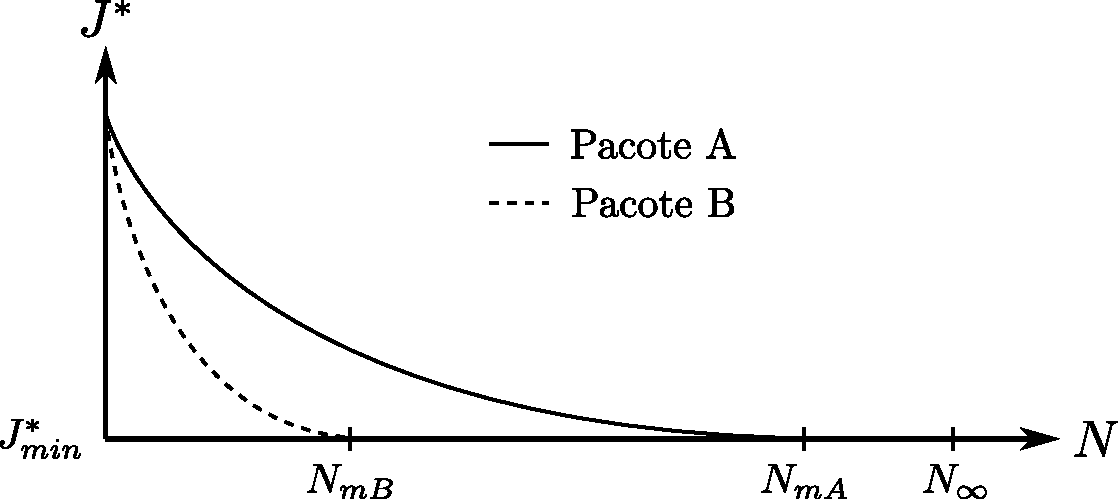
\includegraphics[width=0.75\linewidth]{draw/metodologia/pdf/Nm}
	\captionof{figure}[Relação entre $ N $ e os $ J^* $ atribuídos a dois pacotes quaisquer A e B]{Relação entre $ N $ e os $ J^* $ atribuídos a dois pacotes quaisquer A e B.}
	\label{fig:metodologia:Nm}
	\vspace{\onelineskip}
\end{minipage}

Para que $ N_m $ seja definido é necessário, primeiramente, que o PCO em análise seja resolvido $ n_m $ vezes, considerando-se, a cada execução, um $ N $ distinto. Em seguida, computa-se $ \overline{J^*} $ a partir da normalização de $ J^* $
%
\begin{equation}
	\overline{J^*} = \frac{J^* - J^*_{min}}{J^*_{max} - J^*_{min}}
\end{equation}
%
em que $ J^*_{min} $ e $ J^*_{max} $ são o menor e o maior valor atribuídos a $ J^* $, de forma que $ 0 \leq \overline{J^*} \leq 1 $. Por fim, defini-se $ N_m $ como sendo o menor $ N $ a partir do qual $ \overline{J} < \epsilon_m $, sendo $ \epsilon_m $ um número próximo de zero. No presente trabalho supõe-se $ n_m = 30 $ e $ \epsilon_m = 0,01 $. O processo de normalização de $ J^* $ e a definição de $ \epsilon_m $, que servem de base para a definição de $ N_m $, são representados na Figura \ref{fig:metodologia:Jnorm}. 

\noindent	
\begin{minipage}{\textwidth}
	\vspace{\onelineskip}
	\centering
	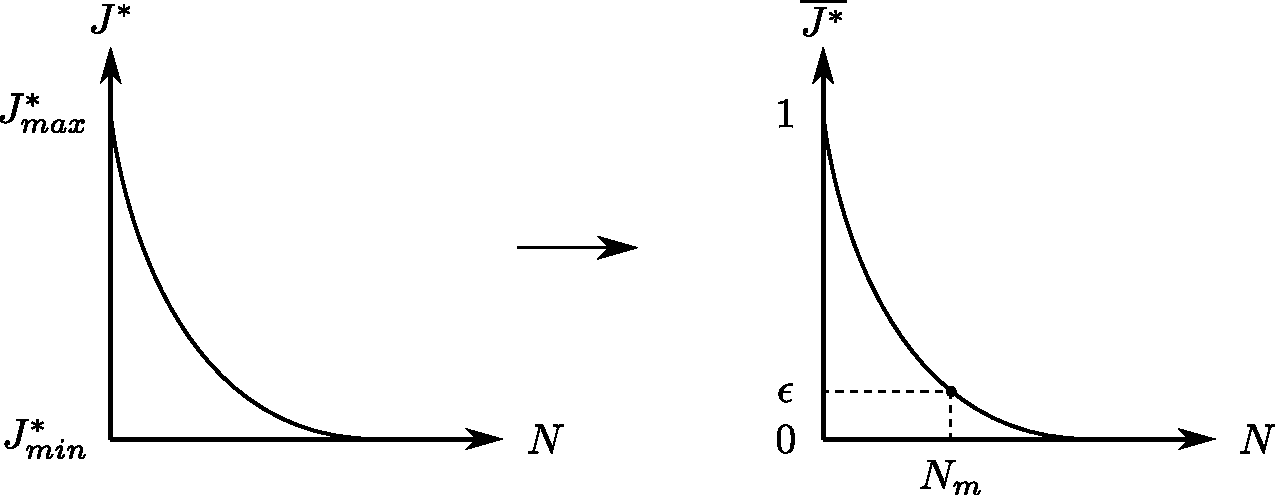
\includegraphics[width=1\linewidth]{draw/metodologia/pdf/Jnorm}
	\captionof{figure}[Representação do processo de normalização de $ J^* $ e da definição de $ \epsilon_m $]{Representação do processo de normalização de $ J^* $ e da definição de $ \epsilon_m $, que servem de base para a definição de $ N_m $.}
	\label{fig:metodologia:Jnorm}
	\vspace{\onelineskip}
\end{minipage}

\todo[inline, size=normalsize, color=pink]{Como estão organizadas as seções do capítulo de resultados}

Os estudos de caso que servem de base para a elaboração do estudo comparativo apresentado no presente trabalho são detalhados nas seções do Capítulo \ref{sec:resultados}. Cada seção se encontra organizada da seguinte maneira:
%
\begin{itemize}
	\item Considerações gerais acerca do estudo de caso em análise;
	\item Formulação da função objetivo, da dinâmica e das restrições associadas ao estudo de caso em análise;
	\item Apresentação dos dados que servem de base para a determinação de $ N_m $;
	\item Análise dos resultados obtidos por meio do emprego de cada um dos pacotes avaliados, considerando-se $ N = N_m $;
	\item Apresentação das trajetórias de estados e controles obtidas a partir da resolução do estudo de caso em análise;
	\item Análise da sensibilidade de $ t_p $ e $ n_{aval} $ ao aumento de $ N $ para cada um dos pacotes avaliados.
\end{itemize} 

Como já foi mencionado anteriormente, o estudo comparativo realizado no presente trabalho é baseado na avaliação de três pacotes: o $ PSOPT $, o $ FALCON $ e o $ COPILOTS $. Uma vez que o $ PSOPT $ e o $ COPILOTS $ possibilitam a utilização de mais de um tipo de colocação, adotam-se os índices $ t $, $ h $ e $ l $ para indicar qual método foi empregado na obtenção de uma dada solução. Esses índices fazem referência à colocação trapezoidal, à colocação Hermite-Simpson, e à colocação pseudo-espectral respectivamente. Para indicar, por exemplo, que uma determinada solução foi obtida empregando-se o $ PSOPT $ e a colocação trapezoidal, atribui-se o rótulo $ PSOPT_t $ à mesma. 

Por fim, ressalta-se que há diversos parâmetros de ajuste associados a cada um dos pacotes avaliados. Assim sendo, seria uma tarefa praticamente impossível verificar a influência de cada um desses parâmetros e ajustá-los de forma que cada execução levasse à melhor solução possível. Logo, recomenda-se que um estudo comparativo se baseei nos valores padrão atribuídos a cada parâmetro \cite{mittelmann_benchmarking_1998}, e, de fato, são esses os valores adotados na obtenção dos resultados apresentados no Capítulo \ref{sec:resultados}.

\todo[inline, color=pink, size=normalsize]{Configurações do PC utilizado}

As configurações do computador utilizado na aquisição e processamento dos dados apresentados no Capítulo \ref{sec:resultados} se encontram listadas a seguir. 
%
\begin{itemize}
	\item \textbf{Modelo}: Laptop Aspire A515-51G;
	\item \textbf{Processador}: Intel\textsuperscript{\textregistered} Core i7-7500U - Frequência máxima de 3,5 GHz - Topologia Dual Core e tecnologia Hyper-Threading Intel\textsuperscript{\textregistered} (2 núcleos e 4 \textit{threads});
	\item \textbf{Memória RAM}: 8 GB (duas placas de 4 GB) DDR4 - Frequência máxima de 2133 MHz; 
	\item \textbf{Placa gráfica}: NVIDIA GeForce 940MX;
	\item \textbf{Sistema operacional}: Linux 64 bits - Kernel 5.8.0-7630 x86\_64;
	\item \textbf{Distribuições}: Pop!\_OS 20.04 LTS ($ FALCON $ e $ COPILOTS $) e Linux Mint 19.3 LTS ($ PSOPT $).
\end{itemize}

% RESULTADOS E DISCUSSÕES
\chapter{Resultados e discussões}
\label{sec:resultados}
% Introdução do capítulo
Nesse capítulo, os  pacotes $ COPILOTS $, $ PSOPT $ e $ FALCON $ serão avaliados considerando os seguintes estudos de caso:
%
\begin{itemize}
\item Minimização do esforço durante a aceleração de um bloco \cite{becerra_optimal_2008};
\item Problemas singulares: Casos 1 e Caso 2 \cite{jacobson_computation_1970};
\item Minimização do esforço durante o \textit{Swing-up} de um pêndulo invertido \cite{kelly_introduction_2017};
\item Minimização do tempo durante uma manobra de estacionamento \cite{li_time-optimal_2016};
\item Otimização da trajetória de um UAV (\textit{Unmanned Aerial Vehicle}) \cite{toledo_de_azevedo_pseudospectral_2018};
\item Lançamento do foguete Delta III \cite{benson_gauss_2005}.
\end{itemize}

Cabe ressaltar que, conforme discutido anteriormente, estes foram escolhidos por apresentarem diferentes níveis de complexidade. Sendo assim, pode-se dizer que estes reúnem boas características para a validação da metodologia proposta neste trabalho, bem como para avaliar os outros pacotes considerados. 

No decorrer desse capítulo cada um dos estudos de caso são apresentados, formulados matematicamente, as respectivas soluções obtidas são apresentadas e a comparação entre os pacotes é realizada. Ao término deste capítulo é apresentado um consolidado dos resultados obtidos.

% integrador
\section{Minimização do esforço durante a aceleração de um bloco}
\label{sec:resultados:integrador}
\label{sec:singular1}

Nesta aplicação considera-se a minimização da força $ F(t) $ empregada durante a aceleração de um bloco com massa $ m $. Partindo do repouso em um ponto de origem, o bloco deve atingir, após $ t_f $ segundos, a velocidade $ v_f $ e a posição final $ d_f $, conforme apresentado na  Figura \ref{fig:integrador:variaveis} \cite{becerra_optimal_2008}.

\noindent
\begin{minipage}{\textwidth}
	\vspace{\onelineskip}
	\centering
	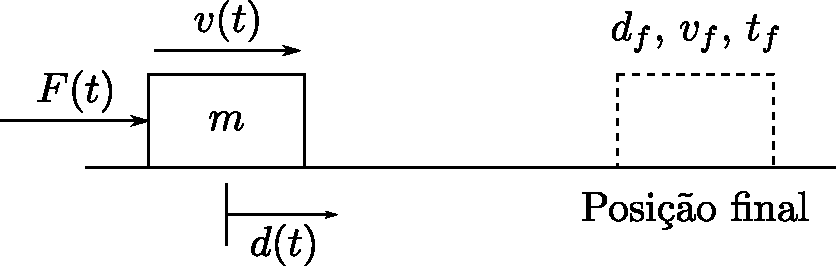
\includegraphics[width=0.6\linewidth]{draw/resultados/pdf/bloco}
	\captionof{figure}[Representação esquemática do problema do bloco]{Representação esquemática do problema da aceleração de um bloco ($ d(t) $ e $ v(t) $ representam, respectivamente, a posição e a velocidade).}
	\label{fig:integrador:variaveis}
	\vspace{\onelineskip}
\end{minipage}

A função objetivo ($J$) a ser minimizada é definida como: 
%
\begin{equation}
	\label{eq:integrador:J}
	J = \int_{0}^{t_f} F^2(t) dt
\end{equation}

A dinâmica do bloco é descrita pelo sistema de equações diferenciais:
%
\begin{subequations}
\begin{equation}
\label{eq:integrador:dinamica}
\dot{d}(t) = v(t),\;\;d(0)=0\;\text{m}
\end{equation}
\vspace{-0.75cm}
\begin{equation}
\dot{v}(t) = \frac{F(t)}{m},\;\;v(0) = 0 \; \text{m/s}
\end{equation}
\end{subequations}
%
em que $ \mathbf{x}(t) = \begin{bmatrix} d(t) & v(t) \end{bmatrix}^T $ são as variáveis de estados do sistema e $ F(t) $ é a variável de controle. Para esta aplicação são considerados os seguintes parâmetros \cite{becerra_optimal_2008}: massa do bloco ($ m = 1$ kg), posição final do bloco ($ d_f = 1$ m) e velocidade final do bloco ($ v_f = 1 $ m/s). 

A inicialização dos estados e controles foi deixada a cargo dos pacotes utilizados, sendo que cada um desses implementa essa inicialização de uma forma distinta, conforme discutido anteriormente. \textcolor{red}{Arthur, seria interessante apresentar uma ideia de como isso é feito. Pra não ser repetitivo, devemos colocar estas informações na descrição dos pacotes.} 

Na Figura \ref{fig:integrador:sensibilidade:J} são apresentados os resultados obtidos considerando a influência do número de nós de colocação ($N$), bem como o número mínimo de nós ($ N_m $) requerido para que o pacote encontre a melhor solução reportada na literatura. Além disso, cabe ressaltar que no $ PSOPT $ foram utilizadas as seguintes discretizações: pseudo-espectral ($PSOPT_l$), trapezoidal ($PSOPT_t$) e Hermite-Simpson ($PSOPT_h$). No $ FALCON $ foi utilizado a discretização trapezoidal ($FALCON$). Finalmente, no $COPILOTS$ foram utilizadas discretizações trapezoidal ($COPILOTS_t$) e Hermite-Simpson ($COPILOTS_h$). 

Para realizar esta análise foram considerados um vetor com trinta valores distintos e igualmente espaçados para $N$, sendo que os limites inferior e superior adotados foram 5 e 63, respectivamente. Neste cenário, objetiva-se avaliar a influência do número de nós de colocação $ N $ no valor de $ J $. 

\noindent	
\begin{minipage}{\textwidth}
	\vspace{\onelineskip}
	\centering
	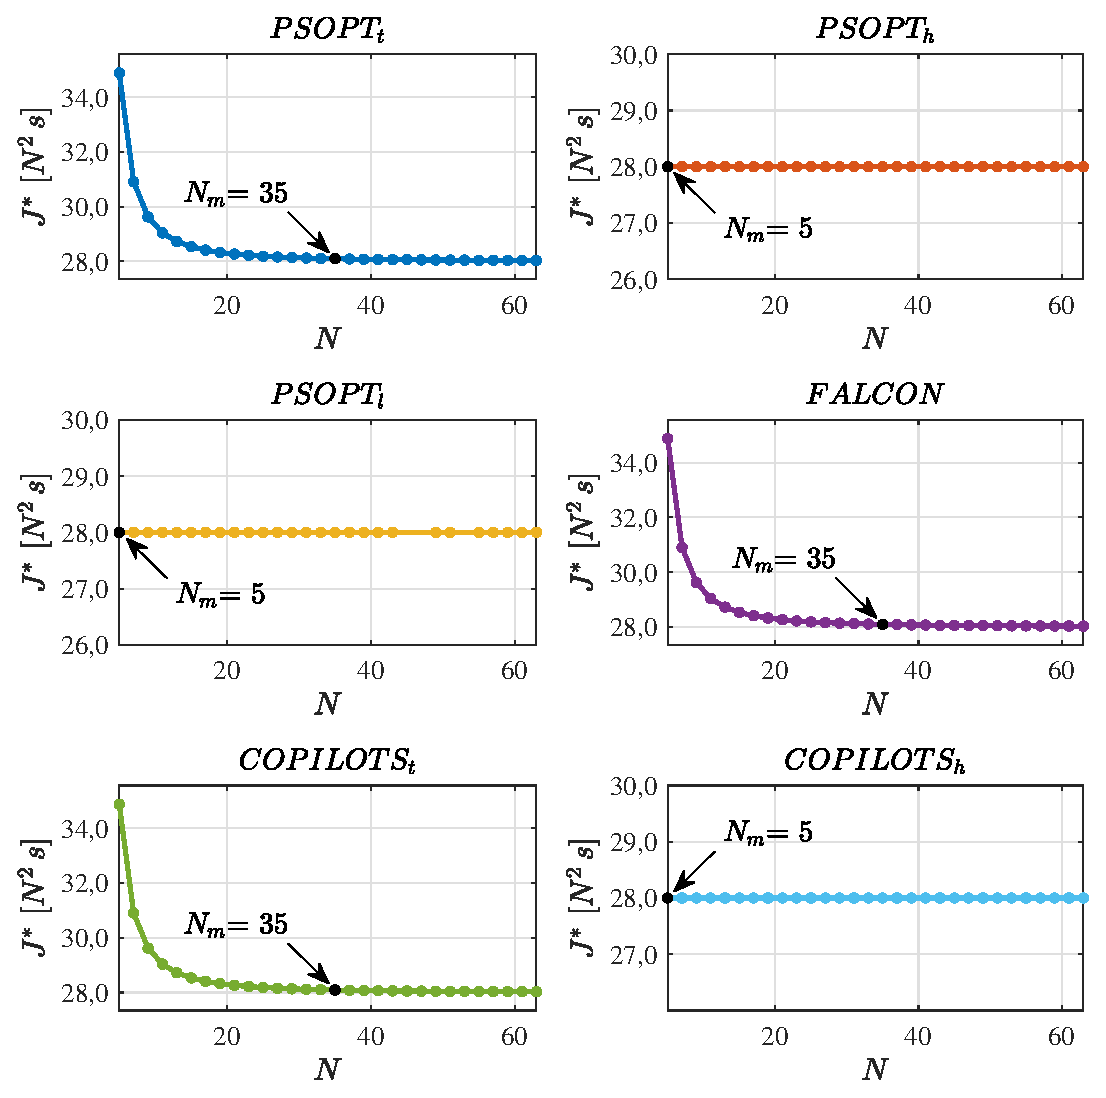
\includegraphics[scale=0.7]{fig/resultados/integrador/sens/J}
\captionof{figure}[Influência do número de nós de colocação no valor da função objetivo para o problema da aceleração de um bloco]{Influência do número de nós de colocação $N$ no valor da função objetivo $J^*$ para o problema da aceleração de um bloco.}
	\label{fig:integrador:sensibilidade:J}
	\vspace{\onelineskip}
\end{minipage}

Nestas figuras pode-se observar que, para o $ PSOPT_t $, $ FALCON $, e o $ COPILOTS_t $ (trapezoidal), o valor de $ J^* $ decresce à medida que $ N $ aumenta e se aproxima da solução analítica conhecida ($ J^* = 28 $). Já para o $ PSOPT_h $ e para o $ COPILOTS_h $ (Hermite-Simpson) e para o $ PSOPT_l $ (pseudo-espectral) observa-se que a solução é encontrada para $ N = 5 $. É importante ressaltar que, para a aplicação do método pseudo-espetral, não foi possível encontrar soluções para $ N $ iguais a 45, 47 e 53. Provavelmente, isto se deve a forma como foram inicializados os perfis das variáveis de estado e controle (\textcolor{red}{Arthur, por isso é importante destacar como essa inicialização é feita. A banca vai te questionar isso. Tem como mudar essa inicialização? Você tentou????. Uma pergunta, o processo de inicialização é o mesmo para todos????}).

Os resultados obtidos para esta aplicação são apresentados na Tabela \ref{tab:integrador:raw} para $ N = N_m$. Nesta tabela, $ t_p $ é o tempo de processamento médio, $ s_t $ é o desvio padrão atribuído a $ t_p $, $ n_{aval} $ é o número de avaliações da função objetivo, $ \Delta c_{max} $ é a máxima violação atribuída às restrições, $ N_s $ é o número de execuções bem sucedidas, e $ N_s\% $ é a relação entre $ N_s $ e o número total de execuções. 

\begin{table}
	\centering
	\caption[Métricas obtidas para o problema da aceleração de um bloco]{Métricas obtidas para o problema da aceleração de um bloco. Os melhores valores para $ N_m $, $ J^* $, $ t_p $, $ n_{aval} $ e $ N_s\% $ encontram-se destacados.}
	\label{tab:integrador:raw}
	\begin{tabular}{@{}ccccccccc@{}}
		\toprule
		Método       & $N_m$                             & $J^*$                                    & $t_p$ {[}$s${]}                         & $s_t$ {[}$s${]} & $n_{aval}$                        & $\Delta c_{max}$                         & $N_s$ & $N_s\%$                                  \\ \midrule
		$PSOPT_t$    & 35                                & 28,09170                                 & 0,31331                                 & 0,00625         & 8                                 & 6,41e-15                                 & 30    & {\color[HTML]{009901} \textbf{100,00\%}} \\
		$PSOPT_h$    & {\color[HTML]{009901} \textbf{5}} & {\color[HTML]{009901} \textbf{28,00000}} & 0,05395                                 & 0,00747         & 15                                & 4,44e-16                                 & 30    & {\color[HTML]{009901} \textbf{100,00\%}} \\
		$PSOPT_l$    & {\color[HTML]{009901} \textbf{5}} & {\color[HTML]{009901} \textbf{28,00000}} & 0,03791                                 & 0,00977         & {\color[HTML]{009901} \textbf{5}} & 7,77e-16                                 & 27    & 90,00\%                                  \\
		$FALCON$     & 35                                & 28,09167                                 & {\color[HTML]{009901} \textbf{0,03663}} & 0,00279         & 6                                 & 2,08e-16 & 30    & {\color[HTML]{009901} \textbf{100,00\%}} \\
		$COPILOTS_t$ & 35                                & 28,09167                                 & 0,52875                                 & 0,01817         & 1404                              & 1,57e-13                                 & 30    & {\color[HTML]{009901} \textbf{100,00\%}} \\
		$COPILOTS_h$ & {\color[HTML]{009901} \textbf{5}} & {\color[HTML]{009901} \textbf{28,00000}} & 0,18729                                 & 0,01770         & 600                               & 3,05e-13                                 & 30    & {\color[HTML]{009901} \textbf{100,00\%}} \\ \bottomrule
	\end{tabular}
\end{table}

Nesta tabela observa-se que foi necessário um maior valor para $ N $ para os pacotes que fazem uso da colocação trapezoidal ($ PSOPT_t $, $ FALCON $ e $ COPILOTS_t $) em comparação com os outros tipos de abordagens. Essa diferença se deve às características numéricas inerentes a cada método. Além disso, observa-se que os valores de $ J^* $ atribuídos às soluções obtidas por meio da colocação trapezoidal são bastante próximos uns dos outros.

Os maiores tempos de processamento foram atribuídos às soluções obtidas por meio do $ PSOPT_t $ e do $ COPILOTS_t $, uma vez que nesses casos foi utilizada uma quantidade maior de nós de colocação. Em contrapartida, o menor $ t_p $ foi encontrado pelo $ FALCON $. Esse comportamento se deve à capacidade que esse pacote possui de empregar ferramentas simbólicas na geração de derivadas analíticas, tanto para a função objetivo quanto para as restrições, o que leva a uma diminuição na quantidade de iterações despendida na obtenção da solução do problema em análise. A essa diminuição, está associada uma redução no tempo de processamento, mesmo quando utilizados muitos nós de colocação. Os tempos de processamento associados ao $ PSOPT_h $, $ PSOPT_l $, e $ FALCON $ foram bastante próximo e, consideravelmente, menores que aqueles requeridos pelo $ PSOPT_t $, $ COPILOTS_t $, e $ COPILOTS_h $. Vale ressaltar que, às soluções obtidas pelo $ COPILOTS $, normalmente estão associados a altos tempos de processamento, uma vez que o pacote utiliza o SQP e é escrito em Matlab\textsuperscript{\textregistered}.

Os valores de $ n_{aval} $ associados ao $ COPILOTS $, independentemente do tipo de colocação considerado, foram bem maiores que aqueles observados nos demais métodos avaliados, uma vez que o pacote faz uso do SQP. Observou-se também que nem sempre $ t_p $ está diretamente relacionado a $ n_{aval} $. Por exemplo, o tempo de processamento associado ao $ PSOPT_t $ é maior que aquele requerido pelo $ PSOPT_h $. Todavia, é o $ PSOPT_h $ que está associado com o maior $ n_{aval} $. Observa-se o mesmo comportamento quando são comparados os resultados obtidos pelo $ COPILOTS_t $ e pelo $ COPILOTS_h $. 

Por fim, ressalta-se que, utilizando qualquer um dos métodos, é possível obter soluções que satisfaçam as restrições do problema para quase todo $ N $. De fato, a $ N_s\% $ foram atribuídos valores iguais, ou bem próximos, a 100\%, enquanto $ \Delta c_{max} $ foi igual a  zero em todas estas execuções. Esse resultado se deve à simplicidade do problema, que não possui restrições terminais ou de caminho, o que na prática, implica em um problema mais simples. 

As trajetórias de estados considerando $ N = N_m $ são apresentadas nas Figuras \ref{fig:integrador:x:d} e \ref{fig:integrador:x:v}, e as trajetórias de controle na Figura \ref{fig:integrador:u:F}. A partir destes resultados constata-se que as trajetórias obtidas por cada um dos pacotes avaliados se mostraram similares. 

\noindent
\begin{minipage}{\textwidth}
	\vspace{\onelineskip}
	\centering
	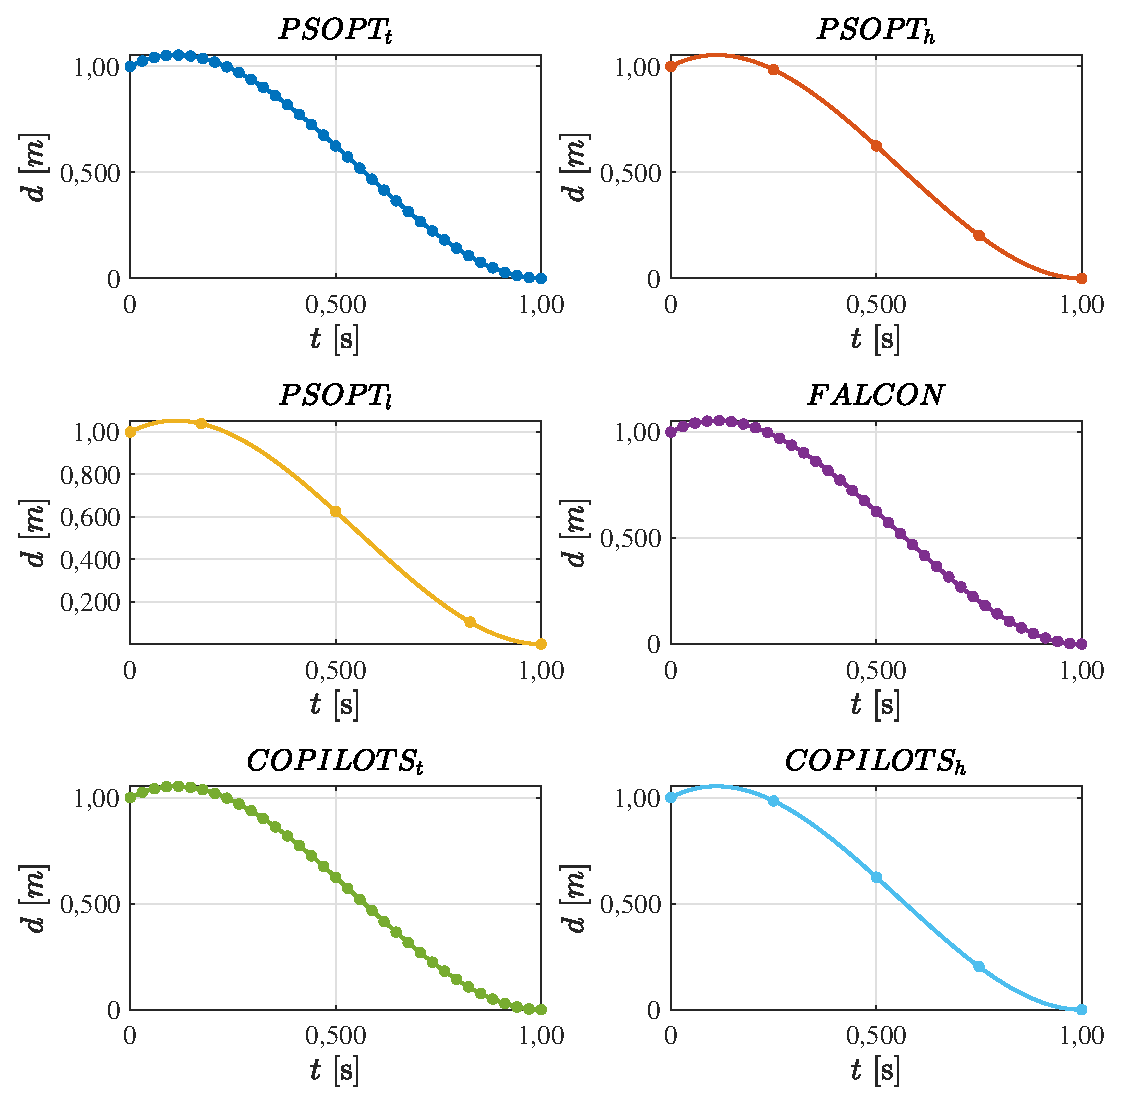
\includegraphics[scale=0.7]{fig/resultados/integrador/traj/x/d}
	\captionof{figure}[Variável de estado $d(t)$ para o problema da aceleração de um bloco]{Variável de estado $d(t)$ para o problema da aceleração de um bloco. Os pontos em cada um dos gráficos representam os valores discretizados, enquanto as linhas contínuas representam as trajetórias interpoladas.}
	\label{fig:integrador:x:d}
	\vspace{\onelineskip}
\end{minipage}

\noindent
\begin{minipage}{\textwidth}
	\vspace{\onelineskip}
	\centering
	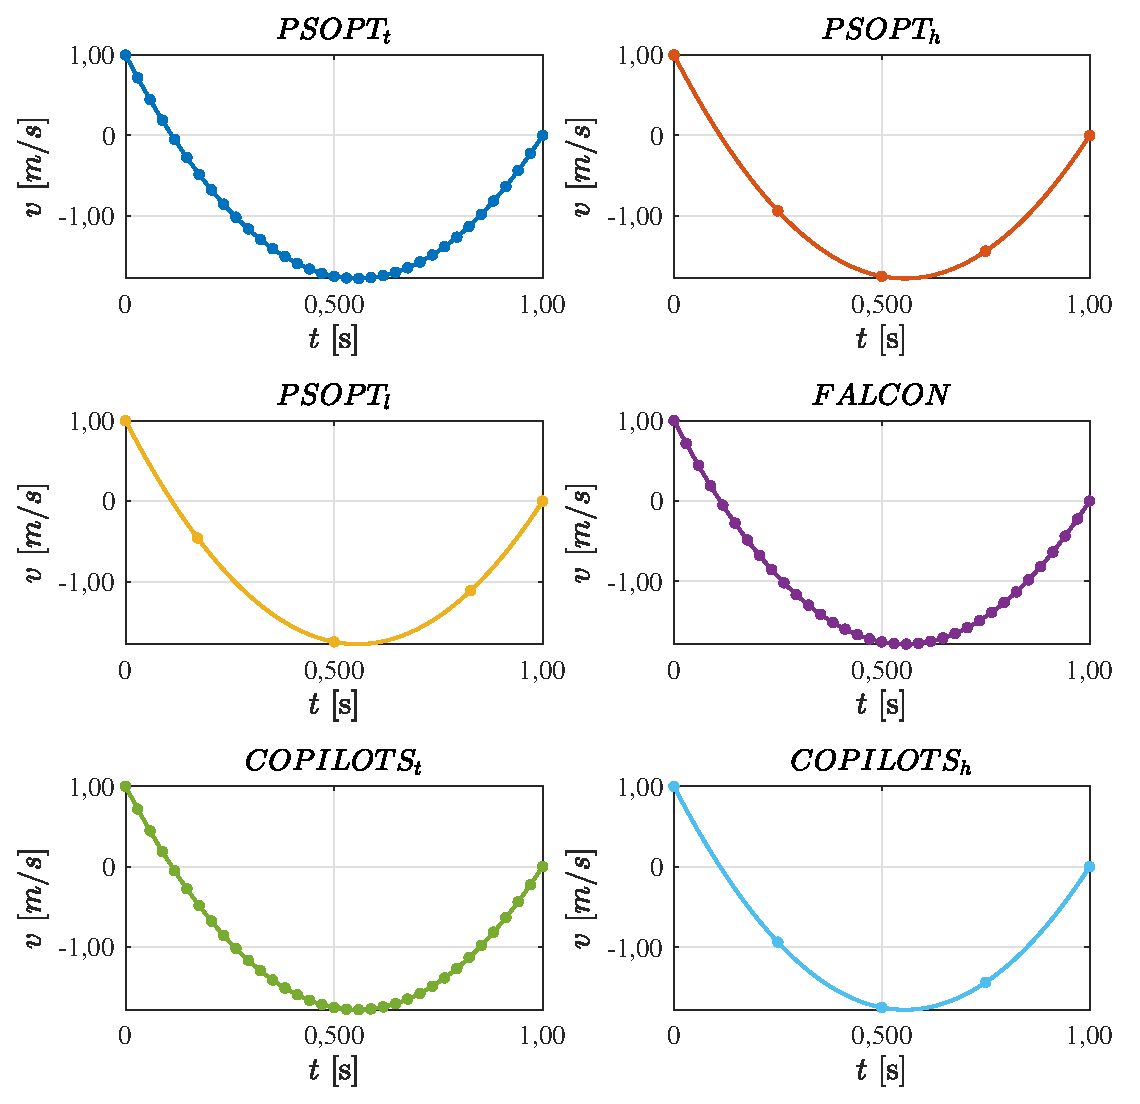
\includegraphics[scale=0.7]{fig/resultados/integrador/traj/x/v}
	\captionof{figure}[Variável de estado $v(t)$ para o problema da aceleração de um bloco]{Variável de estado $v(t)$ para o problema da aceleração de um bloco. Os pontos em cada um dos gráficos representam os valores discretizados, enquanto as linhas contínuas representam as trajetórias interpoladas.}
	\label{fig:integrador:x:v}
	\vspace{\onelineskip}
\end{minipage}

A influência do aumento do número de nós de colocação no tempo de processamento e no número de avaliações da função objetivo são apresentadas nas Figuras \ref{fig:integrador:sensibilidade:t} e \ref{fig:integrador:sensibilidade:naval}, respectivamente. Acima de cada um dos gráficos são apresentadas as diferenças entre os valores máximo e mínimo associados à métrica em questão ($ t_p $ ou $ n_{aval} $), isto é: $ \Delta t_p = \max\{t_p\} - \min\{t_p\} $ e $ \Delta n_{aval} = \max\{n_{aval}\} - \min\{n_{aval}\} $. Os pontos nos gráficos representam os valores obtidos para $ t_p $ (e $ n_{aval} $) em cada nó de colocação, enquanto as linhas contínuas representam curvas de tendência, obtidas por meio de regressões lineares, sendo a sua concordância avaliada de acordo com o coeficiente de determinação ($R^2$). Os valores de $ N $ empregados na geração desses dados são iguais àqueles considerados na computação da relação entre $ J^* $ e $ N $. 

\noindent
\begin{minipage}{\textwidth}
	\vspace{\onelineskip}
	\centering
	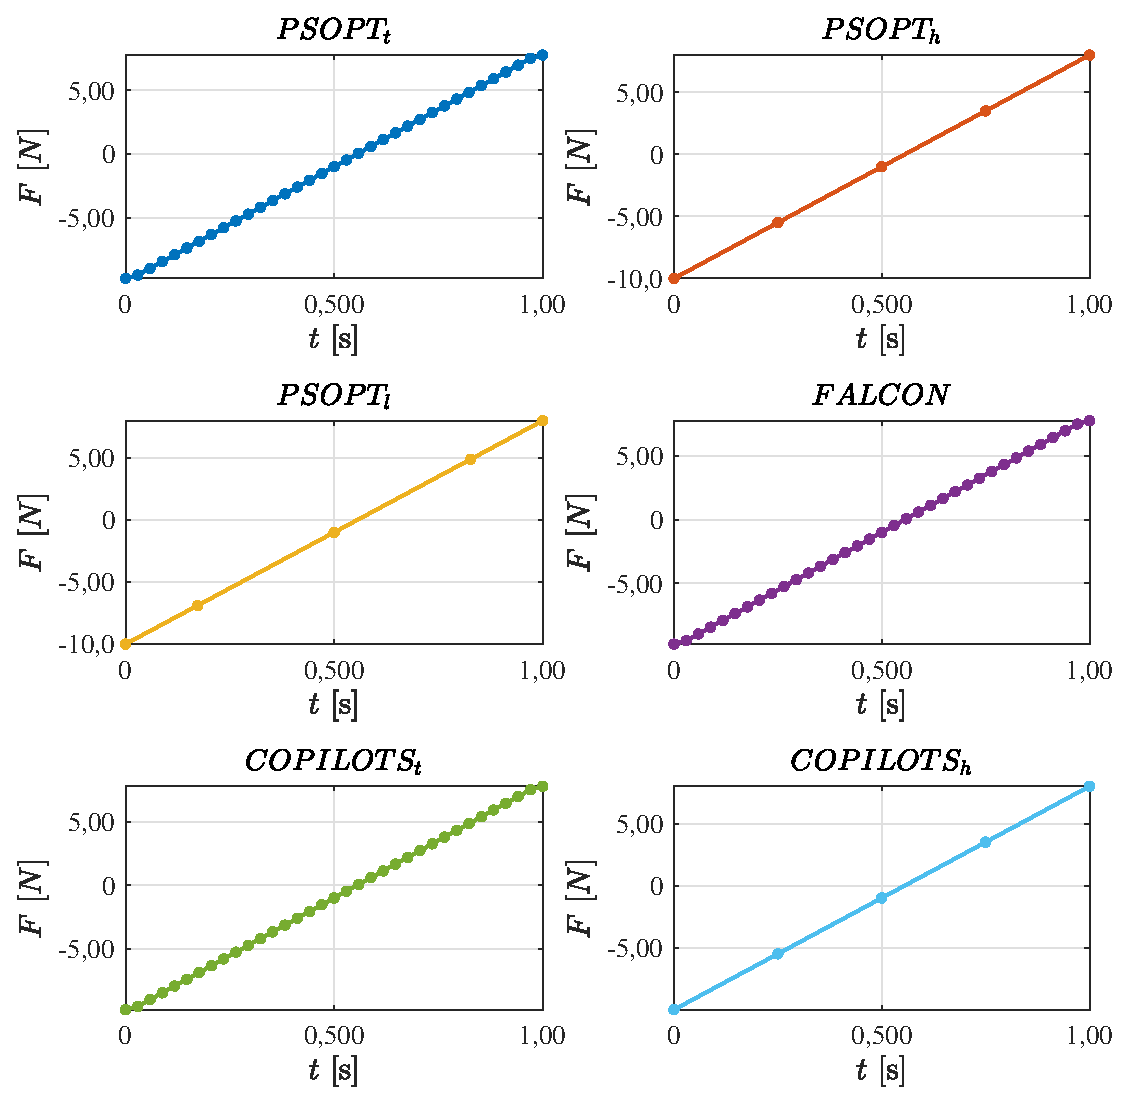
\includegraphics[scale=0.7]{fig/resultados/integrador/traj/u/F}
	\captionof{figure}[Variável de controle $F(t)$ para o problema da aceleração de um bloco]{Variável de controle $F(t)$ para o problema da aceleração de um bloco. Os pontos em cada um dos gráficos representam os valores discretizados, enquanto as linhas contínuas representam as trajetórias interpoladas.}
	\label{fig:integrador:u:F}
	\vspace{\onelineskip}
\end{minipage}

De forma geral nesta figura observa-se o aumento do número de nós de colocação implicam, como esperado, no aumento do tempo de processamento. Em relação ao $ PSOPT_t $ e ao $ PSOPT_h $, estes apresentam tempos de processamento similares e bem inferiores em relação ao $ PSOPT_l$. Já para o $ COPILOTS_t$ observam-se, em média, tempos de processamentos bem distintos em relação ao $ COPILOTS_h$ e aos outros pacotes. Este maior tempo de processamento esta relacionado à solução do PPNL resultante da etapa de discretização. Já para o $ FALCON $ observa-se que este pacote se mostrou muito pouco sensíveis ao aumento de $ N $. Tal fato pode ser justificado ao uso de ferramentas simbólicas na obtenção de derivadas analíticas. De forma geral, apesar das diferenças entre os tempos de processamentos médios observados, considera-se que ambos os pacotes foram eficientes na resolução do problema em questão, visto que a magnitude dos tempos médios requeridos são condizentes com os esperados.

\noindent
\begin{minipage}{\textwidth}
	\vspace{\onelineskip}
	\centering
	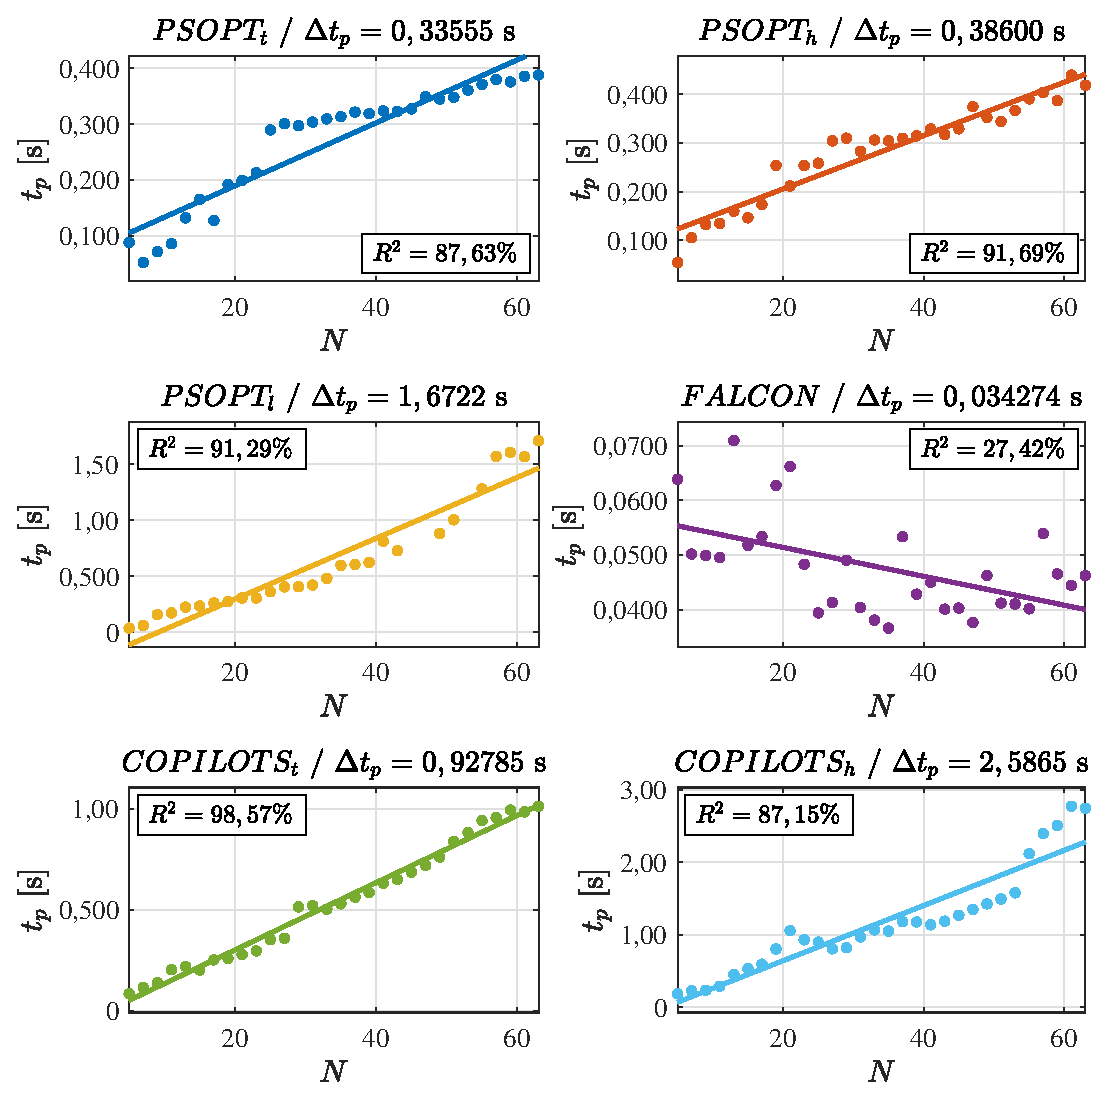
\includegraphics[scale=0.7]{fig/resultados/integrador/sens/t}
	\captionof{figure}[Relação entre o tempo de processamento e o número de nós de colocação para o problema da aceleração de um bloco]{Relação entre o tempo de processamento $ t_p $ e o número de nós de colocação $ N $ para o problema da aceleração de um bloco.}
	\label{fig:integrador:sensibilidade:t}
	\vspace{\onelineskip}
\end{minipage}

Com relação ao número de avaliações da função objetivo ($ n_{aval} $), a variação observada para este parâmetro foi praticamente a mesma para o $ PSOPT_t$, $ PSOPT_h$ e $FALCON$. Já observa-se um aumento significativo para o $ PSOPT_l$ em relação a estes. Os maiores valores para estas variações são observadas para as duas configurações do $COPILOTS$. Este incremento no valor deste parâmetro está associado à solução do PPNL, conforme destacado anteriormente para a análise do  tempo de processamento. Naturalmente, com o aumento no número de nós tem-se o aumento do parâmetro $n_{aval}$, conforme pode ser observado para o $ PSOPT_l$, $COPILOTS_t$ e $COPILOTS_h$. Todavia, para os pacotes $ PSOPT_t$, $ PSOPT_h$ e o $FALCON$, é possível observar uma pequena flutuação no valor de $ n_{aval} $ quando $N$ aumenta. Isto não quer dizer que, para estas variantes, o aumento na discretização do método numérico implique na redução do número de avaliações requeridas, mas apenas que existe uma flutuação neste valor que é função das condições iniciais associadas, bem como na estratégia implementada em cada para a resolução do PCO.

\noindent
\begin{minipage}{\textwidth}
	\vspace{\onelineskip}
	\centering
	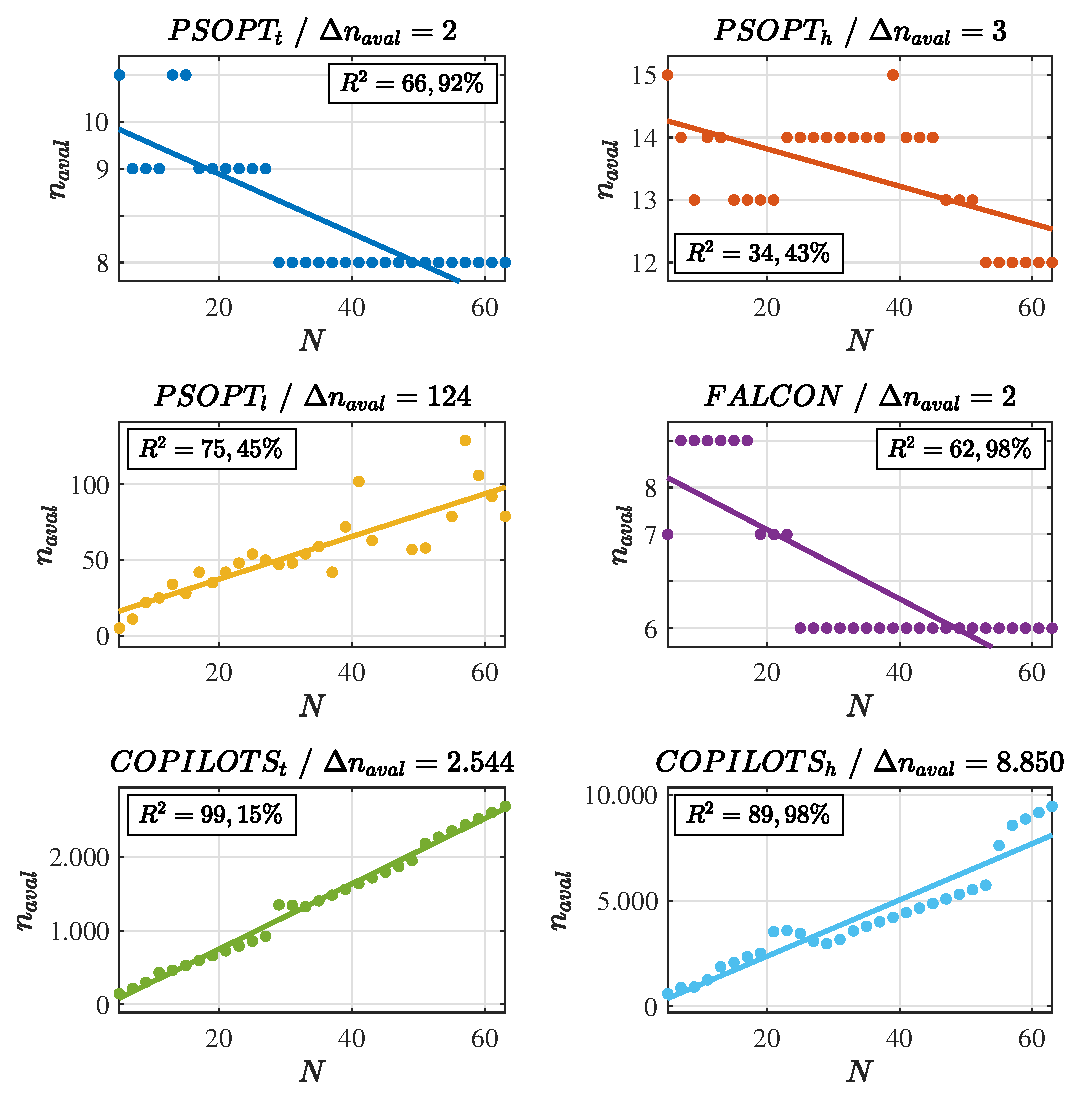
\includegraphics[scale=0.7]{fig/resultados/integrador/sens/eval}
	\captionof{figure}[Relação entre o número de avaliações da função objetivo e o número de nós de colocação para o problema da aceleração de um bloco]{Relação entre o número de avaliações da função objetivo $ n_{aval} $ e o número de nós de colocação $ N $ para o problema da aceleração de um bloco.}
	\label{fig:integrador:sensibilidade:naval}
	\vspace{\onelineskip}
\end{minipage}

% Problemas singulares
\label{sec:resultados:singulares}
\section{Problemas singulares}
Os estudos de caso singulares (Casos 1 e 2) avaliados nessa seção foram propostos por \citeonline{jacobson_computation_1970} e utilizados na validação de um método proposto pelo autor para solução de PCOs singulares. Desde então, vários outros autores \cite{nascentes_resolucao_2012, iasbeck_resolucao_2020} os têm empregado com essa mesma finalidade. % No Apêndice \ref{apd:singulares}, demonstra-se que os estudos de caso em questão são de fato singulares. 

Verifica-se por meio da análise das soluções reportadas por \citeonline{jacobson_computation_1970} (ver as Figuras \ref{fig:singular1:jacobson} e \ref{fig:singular2:jacobson}), que os perfis de controle associados às soluções de cada um dos estudos de caso são descontínuos em $ t \approx 1,5$ s. Assim, espera-se que a presença de descontinuidades nas trajetórias de controle dificulte a resolução desses problemas, principalmente ao se aplicar a colocação pseudo-espectral, uma vez que desaconselha-se o emprego desse tipo de abordagem para a determinação de trajetórias não suaves \cite{becerra_tutorial_2010}. 

\noindent	
\begin{minipage}{\textwidth}
	\vspace{\onelineskip}
	\centering
	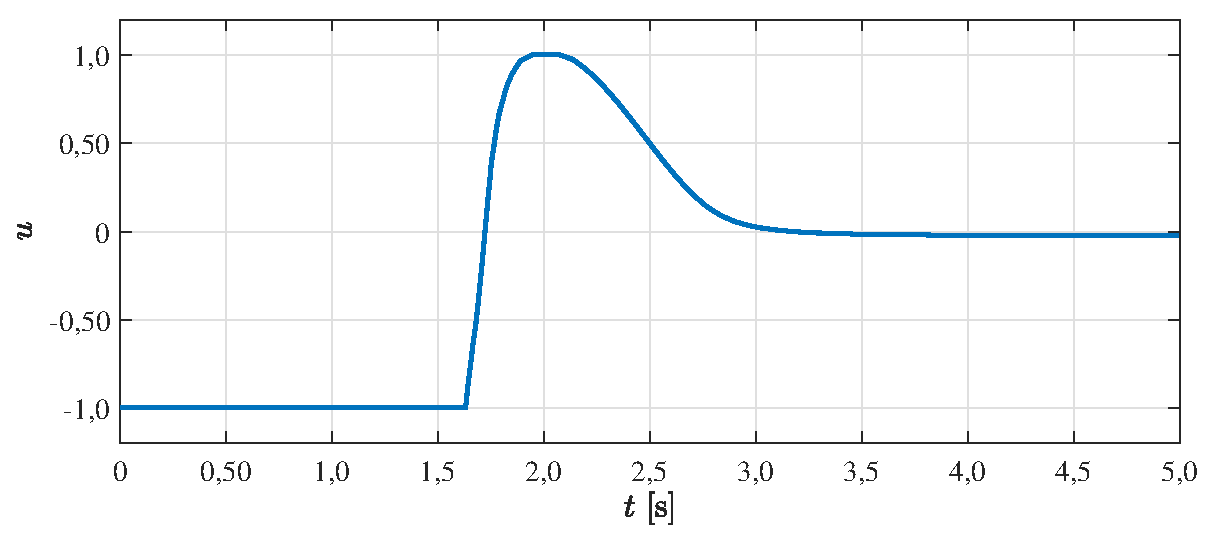
\includegraphics[scale=0.7]{fig/resultados/singular1/obs/original}
	\captionof{figure}[Solução do problema singular 1 reportada na literatura]{Resultado reportado por \citeonline{jacobson_computation_1970} para o estudo de caso descrito na Seção \ref{sec:singular1}.}
	\label{fig:singular1:jacobson}
	\vspace{\onelineskip}
\end{minipage} 

\noindent	
\begin{minipage}{\textwidth}
	\vspace{\onelineskip}
	\centering
	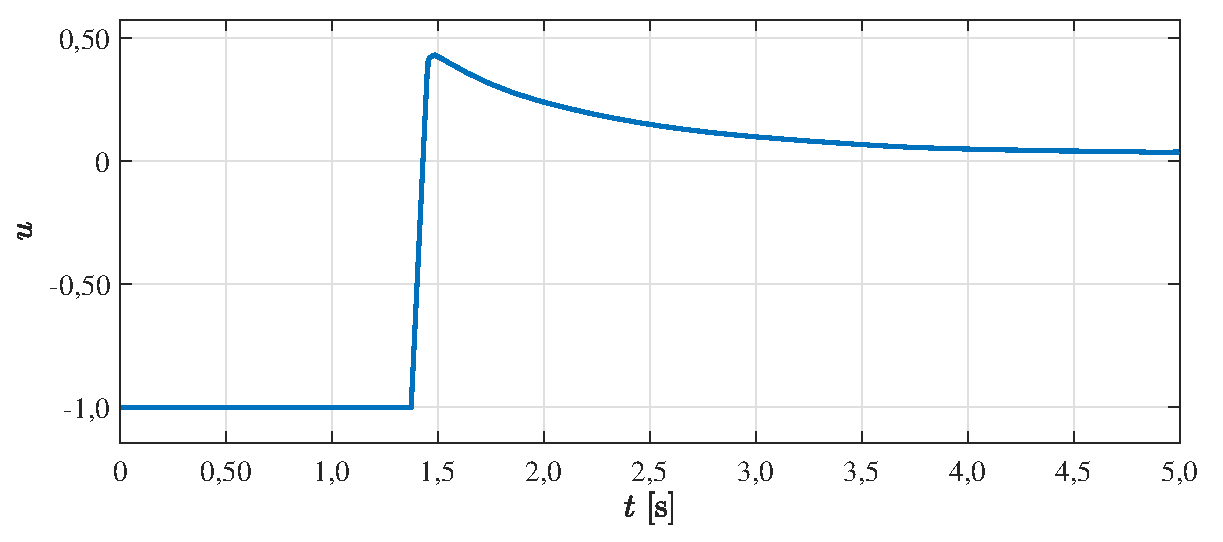
\includegraphics[scale=0.7]{fig/resultados/singular2/obs/original}
	\captionof{figure}[Solução do problema singular 2 reportada na literatura]{Resultado reportado em \citeonline{jacobson_computation_1970} para o estudo de caso descrito na Seção \ref{sec:singular2}.}
	\label{fig:singular2:jacobson}
	\vspace{\onelineskip}
\end{minipage} 

% singular1
\subsection{Caso 1}
\label{sec:resultados:singular1}
\label{sec:singular1}

Considere a minimização da seguinte função objetivo:
%
\begin{equation}
	\label{eq:singular1:J}
	J = x_3(t_f)
\end{equation}
%
sujeito ao seguinte sistema de equações diferenciais ordinárias, bem como uma restrição para o controle:
%
\begin{equation}
	\label{eq:singular1:dinamica}
	\begin{gathered}
		\dot{x}_1(t) = x_2(t), \;\; x_1(0) = 0\\
		\dot{x}_2(t) = u(t), \;\; x_2(0) = 1 \\
		\dot{x}_3(t) = x_1^2(t), \;\; x_3(0) = 0\\
		-1 \leq |u(t)| \leq 1
	\end{gathered}
\end{equation}
%
em que $t$ é o tempo ($t_f$ é o tempo final) e $\mathbf{x}(t) = \begin{bmatrix} x_1(t) & x_2(t) & x_3(t) \end{bmatrix}^T $ é o vetor de variáveis de estado e $ u(t) $ a variável de controle. 

Conforme comentado para o primeiro exemplo, a estimativa inicial para os perfis de estado e controle foi inicializada de forma \textit{default} por cada um dos pacotes. \textcolor{red}{Arthur, aqui já devemos ter apresentado a metodologia usada por cada pacote para definir o chute. Isto deve ser feito na apresentação de cada um dos pacotes, respectivamente (na revisão bibliográfica e na metodologia, respectivamente.)}

Na Figura \ref{fig:singular1:sensibilidade:J} são apresentadas a influência do melhor valor da função objetivo encontrada $ J^* $ em relação ao número de nós utilizados. Também foi determinado o número mínimo de nós de colocação ($ N_m $) necessários para a convergência do resultado para a solução reportada na literatura. Cabe ressaltar que foram escolhidos 30 valores igualmente espaçados dentro do intervalo [5 150]. 

De forma geral observa-se que, para cada um dos pacotes analisados, a partir de um número mínimo de nós de colocação, sempre foi possível encontrar a solução reportada na literatura, a saber, $ J^* $= \textcolor{red}{Arthur, qual o valor??? coloque a referência base}. Ressalta-se que, empregando os métodos $ PSOPT_t $ ou $ PSOPT_h $, não foi possível determinar a solução para pequenos valores para $N$ (entre 5 e 50, aproximadamente). Além disso, destaca-se que, no caso do $ COPILOTS_h $, optou-se por atribuir a $ N_m $ o $ N $ associado ao menor valor de $ J^* $, uma vez que, após atingir esse valor, o custo ótimo passou a crescer antes de alcançar a convergência. 

Os valores de $ J^* $ associados aos resultados obtidos usando o $ COPILOTS_h $ convergiram rapidamente, o que se deve ao SQP e às características numéricas inerentes à colocação Hermite-Simpson, isto é; maior precisão. Em contrapartida, os valores de $ J^* $ associados ao $ PSOPT_l $ apresentaram uma convergência mais lenta do que aquela observada nos demais métodos. Esse comportamento pode ser justificado pelas propriedades numéricas da colocação pseudo-espectral, cujo emprego na resolução de PCOs que apresentam descontinuidades nos controles não é recomenda \cite{becerra_tutorial_2010}.

Os resultados obtidos pelo $ FALCON $ e pelo $ COPILOTS_t $ se mostraram bem próximos, uma vez que ambos utilizam a colocação trapezoidal. Cabe ressaltar que, nesses casos, foi possível solucionar o PCO mesmo para valores de $ N $ pequenos, algo que não foi possível  utilizando-se o $ PSOPT_t $, que também emprega a colocação trapezoidal. 

\noindent	
\begin{minipage}{\textwidth}
	\vspace{\onelineskip}
	\centering
	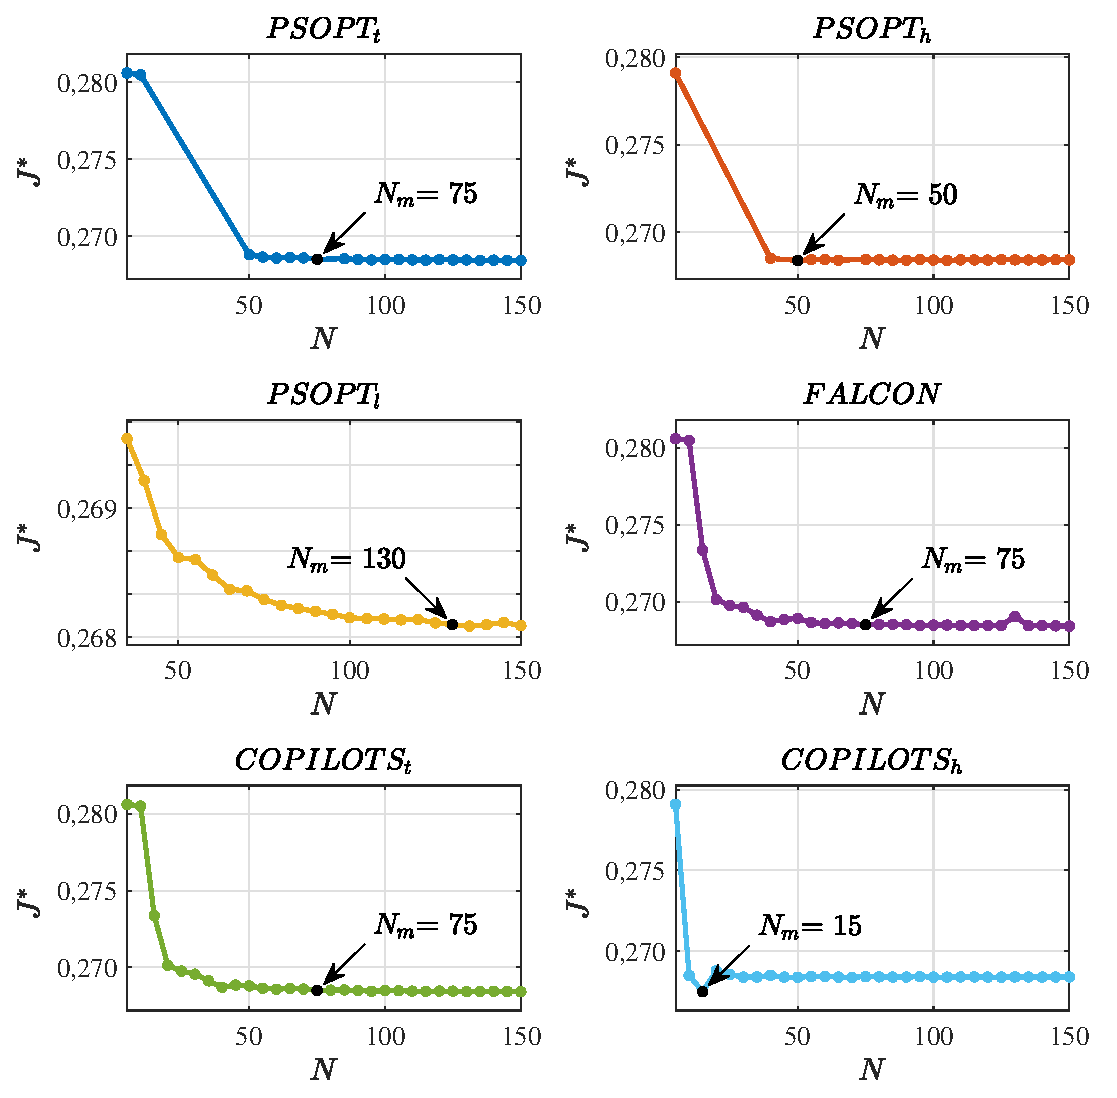
\includegraphics[scale=0.7]{fig/resultados/singular1/sens/J}
	\captionof{figure}[Influência do número de nós de colocação no valor da função objetivo para o problema singular 1]{Influência do número de nós de colocação $ N $ no valor da função objetivo $ J^* $ para o problema singular 1.}
	\label{fig:singular1:sensibilidade:J}
	\vspace{\onelineskip}
\end{minipage}

A Tabela \ref{tab:singular1:raw} apresenta as métricas obtidas por cada um dos pacotes considerando $ N = N_m $. Como destacado no primeiro estudo de caso, $ J^* $ é o valor da função objetivo, $ t_p $ é o  tempo de processamento médio, $ s_t $ é o desvio padrão com relação à  $ t_p $, $ n_{aval} $ é o número de avaliações da função objetivo, $ \Delta c_{max} $ é a máxima violação das restrições, $ N_s $ é o número de execuções bem sucedidas.

\begin{table}
	\centering
	\caption[Métricas obtidas para o problema singular 1]{Métricas obtidas para o problema singular 1. Os melhores valores para $ N_m $, $ J^* $, $ t_p $, $ n_{aval} $ e $ N_s\% $ encontram-se destacados.}
	\label{tab:singular1:raw}
	\begin{tabular}{@{}ccccccccc@{}}
		\toprule
		Método       & $N_m$                              & $J^*$                                   & $t_p$ {[}$s${]}                         & $s_t$ {[}$s${]} & $n_{aval}$                         & $\Delta c_{max}$                         & $N_s$ & $N_s\%$                                  \\ \midrule
		$PSOPT_t$    & 75                                 & 0,26850                                 & 16,30566                                & 0,26206         & 6140                               & 4,44e-12                                 & 22    & 73,33\%                                  \\
		$PSOPT_h$    & 50                                 & 0,26838                                 & 3,28051                                 & 0,18163         & 951                                & 1,99e-07                                 & 22    & 73,33\%                                  \\
		$PSOPT_l$    & 130                                & 0,26846                                 & 29,17814                                & 1,97563         & 429                                & 3,77e-08                                 & 24    & 80,00\%                                  \\
		$FALCON$     & 75                                 & 0,26851                                 & {\color[HTML]{009901} \textbf{0,23411}} & 0,04632         & {\color[HTML]{009901} \textbf{49}} & 5,62e-08                                 & 30    & {\color[HTML]{009901} \textbf{100,00\%}} \\
		$COPILOTS_t$ & 75                                 & 0,26850                                 & 22,39840                                & 0,50176         & 61812                              & 1,02e-09                                 & 30    & {\color[HTML]{009901} \textbf{100,00\%}} \\
		$COPILOTS_h$ & {\color[HTML]{009901} \textbf{15}} & {\color[HTML]{009901} \textbf{0,26749}} & 3,43669                                 & 0,05187         & 16303                              & 3,82e-13 & 30    & {\color[HTML]{009901} \textbf{100,00\%}} \\ \bottomrule
	\end{tabular}
\end{table}

Primeiramente, nota-se nesta tabela que foi necessário um número maior de nós de colocação utilizando-se métodos que fazem uso da colocação trapezoidal ($ PSOPT_t $, $ FALCON $ e $ COPILOTS_t $) em comparação com aqueles que utilizam a colocação Hermite-Simpson. Essa diferença se deve às características numéricas inerentes a cada método. Além disso, observa-se que os valores de $ J^* $ relacionados às soluções obtidas empregando colocação trapezoidal são bastante próximos uns dos outros, enquanto os valores de $ N_m $ a elas associadas são iguais.

O maior valor de $ N_m $ está associado ao $ PSOPT_l $, sendo esse outro indício de que a colocação pseudo-espectral não deve ser empregada na solução de problemas singulares. Aos métodos que utilizam a colocação Hermite-Simpson associam-se os menores valores de $ N_m $, devido às características numéricas inerentes a esse tipo de colocação. O menor valor de $ N_m $ está associado ao $ COPILOTS_h $, provavelmente, por conta do uso que o pacote faz do SQP. Ainda assim, apesar do baixo número de nós de colocação associado ao resultado obtido por meio desse pacote, é a ele que se atribui o menor $ J^* $. 

Ao $ FANCON $ estão associados o menor $ t_p $ e o menor $ n_{aval} $, apesar do $ N_m $ a ele atribuído ter sido maior do que os associados ao $ PSOPT_t $ e ao $ COPILOTS_h $. Esse comportamento se deve, mais uma vez, ao uso que o $ FALCON $ faz de ferramentas simbólicas na obtenção de derivadas analíticas. Os maiores $ t_p $ foram obtidos pelo $ PSOPT_l $ devido ao elevado valor do parâmetro $ N_m $ associado a esse pacote, e ao $ COPILOTS_t $ devido ao uso que o $ COPILOTS $ faz do SQP e às características numéricas inerentes a colocação trapezoidal. Pelas mesmas razões, a utilização do $ COPILOTS $, independentemente do tipo de colocação considerado, está associada a valores de $ n_{aval} $ consideravelmente altos, em comparação com os demais métodos avaliados. Observa-se que nem sempre $ t_p $ está diretamente relacionado ao $ n_{aval} $. Por exemplo, o tempo de processamento associado ao $ PSOPT_t $ é menor que o atribuído ao $ PSOPT_l $. O mesmo pode ser observado em relação ao $ N_m $ e $ n_{aval} $. Ressalta-se ainda que o $ COPILOTS $ e o $ FALCON $ possibilitaram a resolução do problema analisado para qualquer um dos valores de $ N $ adotados. 

Os perfis referente as variáveis de estado e de controle considerando $ N = N_m $ são apresentadas nas Figuras \ref{fig:singular1:x:x1} à  \ref{fig:singular1:u:u}. De forma geral, constata-se que os perfis obtidos por cada um dos pacotes é similar, apesar das leves oscilações observadas nas trajetórias de $ x_1(t) $ e $ x_2(t) $ advindas do emprego do $ PSOPT_l $. 

\noindent
\begin{minipage}{\textwidth}
	\vspace{\onelineskip}
	\centering
	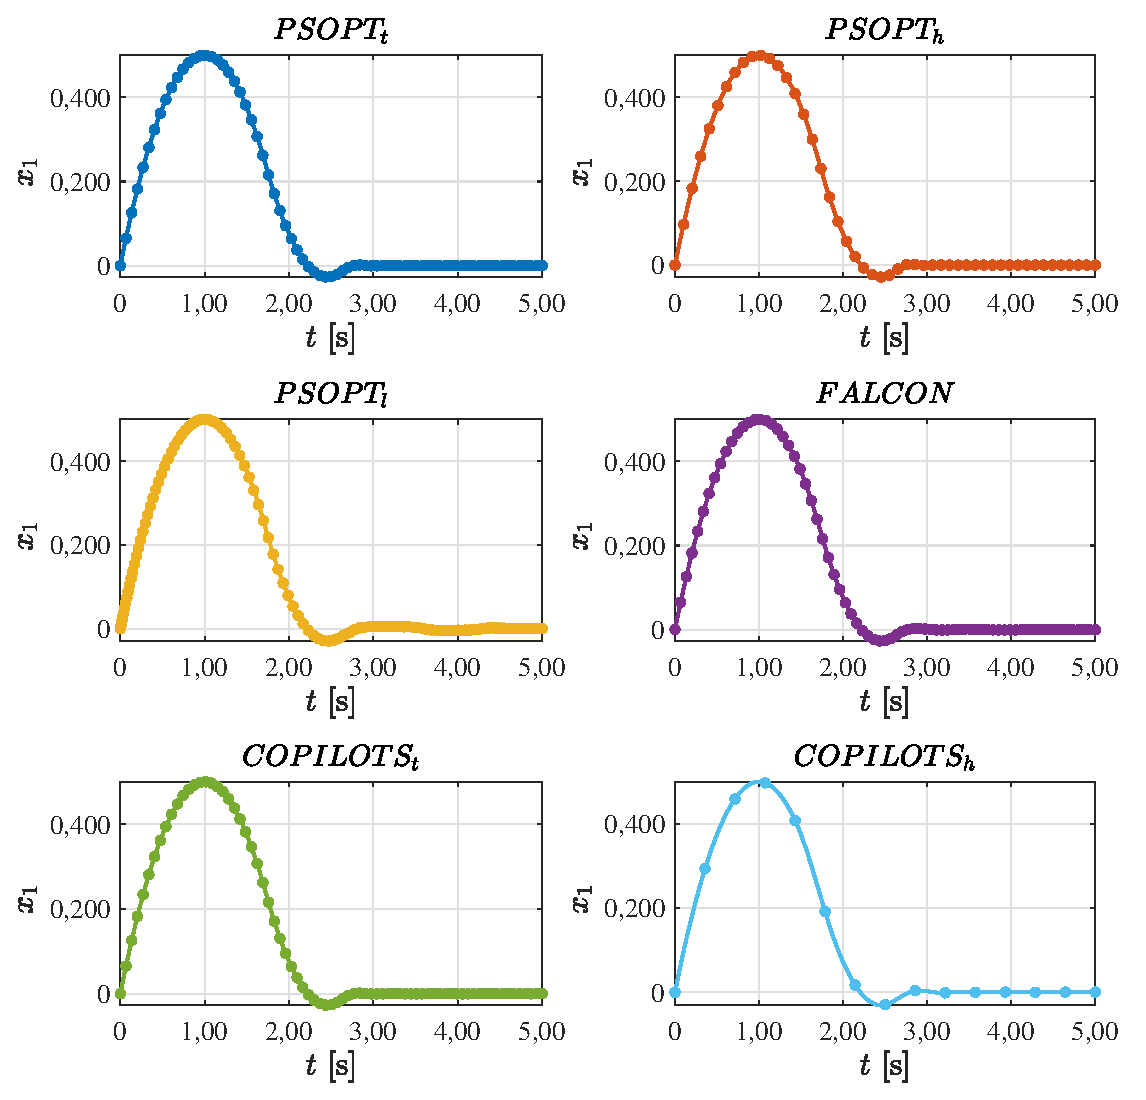
\includegraphics[scale=0.7]{fig/resultados/singular1/traj/x/x_1}
	\captionof{figure}[Variável de estado $x_1(t)$ para o problema singular 1]{Variável de estado $x_1(t)$ para o problema singular 1. Os pontos representam os valores discretizados e as linhas contínuas representam as trajetórias interpoladas.}
	\label{fig:singular1:x:x1}
	\vspace{\onelineskip}
\end{minipage}

Com relação as trajetórias de controle pode-se observar que estas apresentam a mesma tendência, apesar de diferenças em cada um dos pacotes utilizados. Primeiramente, verificam-se descontinuidades nos controles,  em $ t \approx 1,75 \, s $ e $ t \approx 2,5 \, s $, que são inerentes à solução do estudo de caso em análise. Além disso, nota-se que a presença dessas descontinuidades leva ao aparecimento de oscilações nos controles. Dentre as trajetórias de controle obtidas, a mais oscilatória é aquela advinda do emprego do $ PSOPT_l $, o que se deve ao alto $ N_m $ utilizado e às limitações numéricas inerentes à colocação trapezoidal. De fato, leves oscilações podem ser verificadas em todas as trajetórias, principalmente naquelas associadas ao $ PSOPT_t $ e ao $ COPILOTS_t $. Porém, apesar de também empregar a colocação trapezoidal, o $ FALCON $ foi o pacote que possibilitou a obtenção da trajetória mais suave. Tal comportamento pode ser justificado pela precisão dos resultados ao se empregar  ferramentas simbólicas na obtenção de derivadas.

\noindent
\begin{minipage}{\textwidth}
	\vspace{\onelineskip}
	\centering
	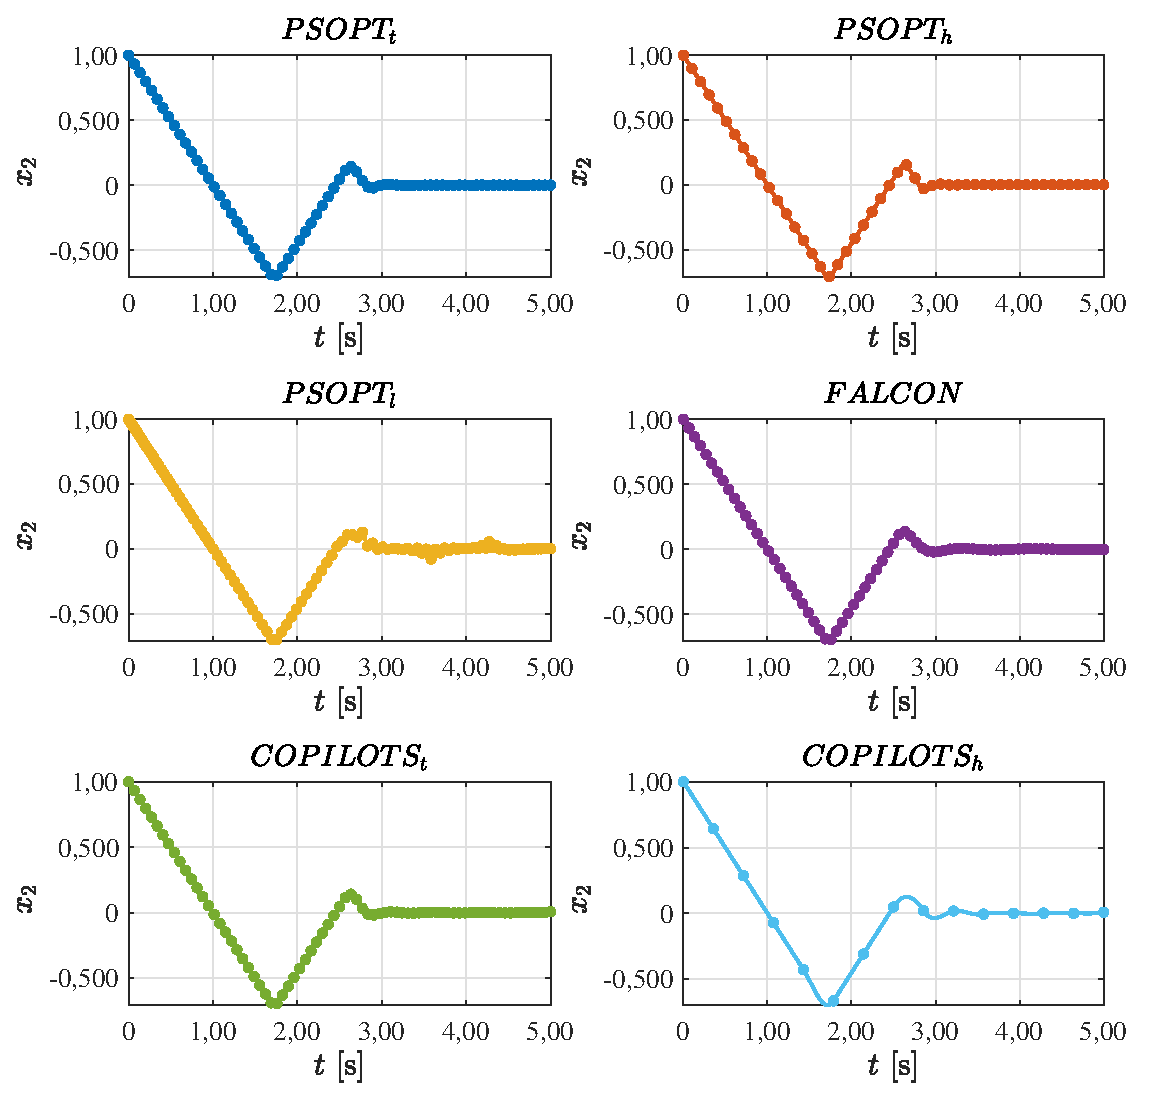
\includegraphics[scale=0.7]{fig/resultados/singular1/traj/x/x_2}
	\captionof{figure}[Variável de estado $x_2(t)$ para o problema singular 1]{Variável de estado $x_2(t)$ para o problema singular 1. Os pontos representam os valores discretizados e as linhas contínuas representam as trajetórias interpoladas.}
	\label{fig:singular1:x:x2}
	\vspace{\onelineskip}
\end{minipage}

Por fim, ressalta-se que as trajetórias de controle interpoladas considerando o $ COPILOTS_h $ e o $ PSOPT_l $, em alguns pontos, desrespeitam as restrições de caminho associadas ao estudo de caso em análise, que impõe que $ -1 \leq u(t) \leq 1 $. Além disso, nota-se o aparecimento de descontinuidades na trajetória atribuída ao $ COPILOTS_h $, em $ t = 2,85 \, s $ e $ t = 3,57 \, s $. Esse comportamento se deve ao tipo de interpolação associada à colocação Hermite-Simpson.

Foi também verificado a influência do aumento no número de nós de colocação tem no tempo de processamento e no número de avaliações da função objetivo, conforme as Figuras \ref{fig:singular1:sensibilidade:t} e  \ref{fig:singular1:sensibilidade:naval}. Nestes gráficos são apresentadas as variações: $ \Delta t_p = \max\{t_p\} - \min\{t_p\} $ e $ \Delta n_{aval} = \max\{n_{aval}\} - \min\{n_{aval}\} $. Os pontos nos gráficos representam os valores atribuídos a $ t_p $ (e a $ n_{aval} $) para cada um dos $ N $ considerados, enquanto as linhas contínuas representam curvas de tendência, obtidas por meio de regressões lineares, em que $R^2$ é o coeficiente de determinação. Os valores de $ N $ empregados na geração desses resultados são iguais àqueles considerados na computação da relação entre $ J^* $ e $ N $. 


\noindent
\begin{minipage}{\textwidth}
	\vspace{\onelineskip}
	\centering
	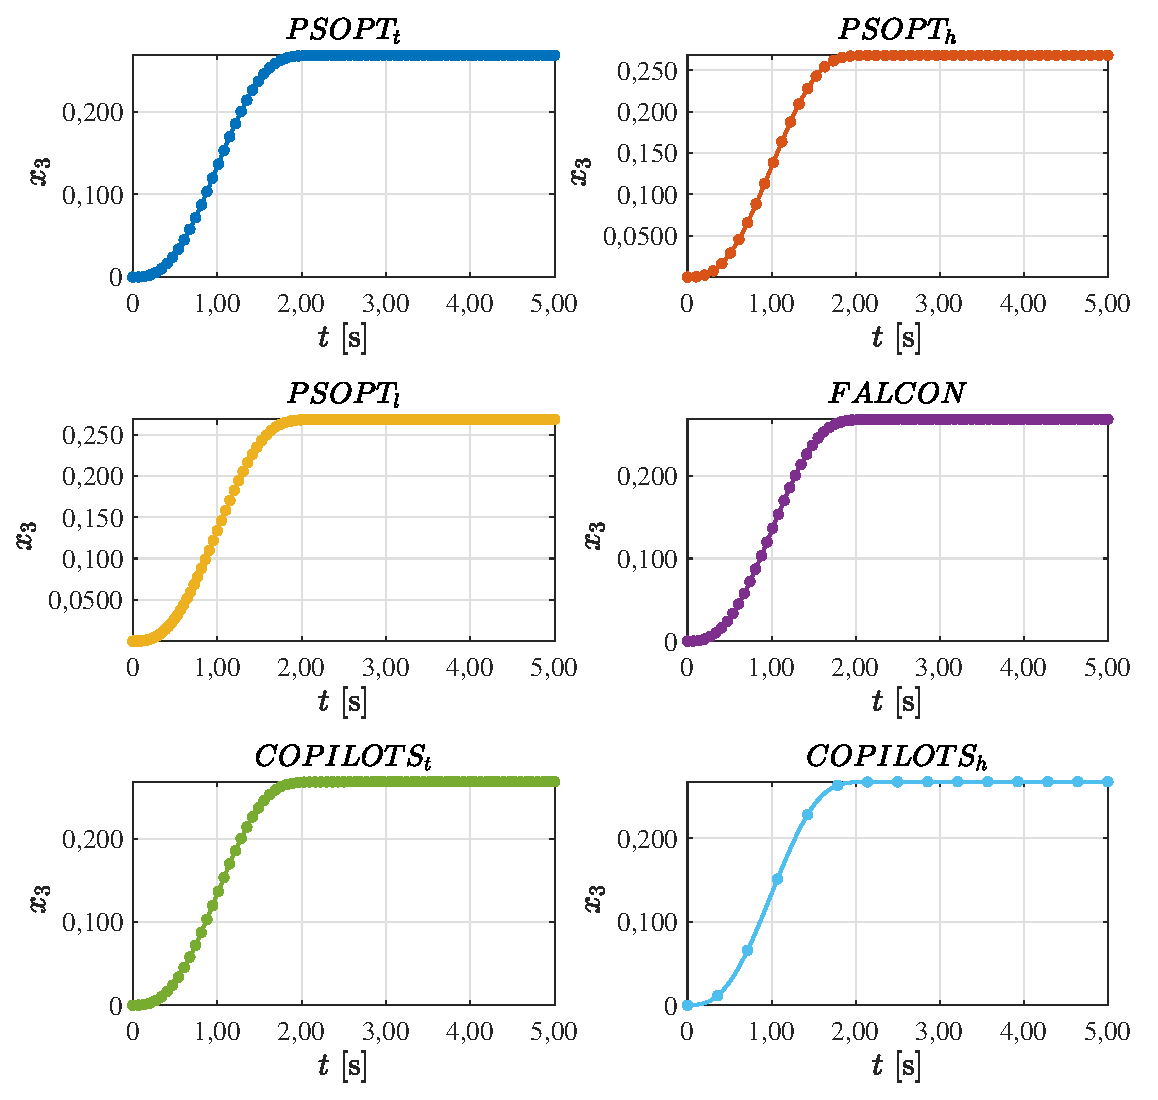
\includegraphics[scale=0.7]{fig/resultados/singular1/traj/x/x_3}
	\captionof{figure}[Variável de estado $x_3(t)$ para o problema singular 1]{Variável de estado $x_3(t)$ para o problema singular 1. Os pontos representam os valores discretizados e as linhas contínuas representam as trajetórias interpoladas.}
	\label{fig:singular1:x:x3}
	\vspace{\onelineskip}
\end{minipage}

Primeiramente, avaliando os resultados obtidos pelo $ COPILOTS $ verifica-se uma relação quadrática entre $ t_p $ e $ N $, e entre $ n_{aval} $ e $ N $. Neste caso, os elevados valores de $ n_{aval} $ e $ t_p $ pode ser justificados pela metodologia empregada para resolver o PPNL. Por outro lado, os resultados indicam que o $ FALCON $ é o método menos sensível a variações em $ N $, uma vez que, a partir do seu emprego, verificaram-se os menores valores de $ \Delta t_p $ e $ \Delta n_{aval} $ em comparação com os demais métodos em análise. Observa-se ainda que os $ t_p $ associados ao $ PSOPT_l $ são mais sensíveis ao aumento de $ N $ que aqueles atribuídos ao $ PSOPT_t $ e ao $ PSOPT_h $, considerando-se o alto $ \Delta t_p $ associado ao $ PSOPT_l $. No entanto, observou-se que o inverso é válido quando analisada a sensibilidade de $ n_{aval} $, tendo em vista o baixo $ \Delta n_{aval} $ atribuído ao $ PSOPT_l $ em comparação com aqueles associados ao $ PSOPT_t $ e ao $ PSOPT_h $.

\noindent
\begin{minipage}{\textwidth}
	\vspace{\onelineskip}
	\centering
	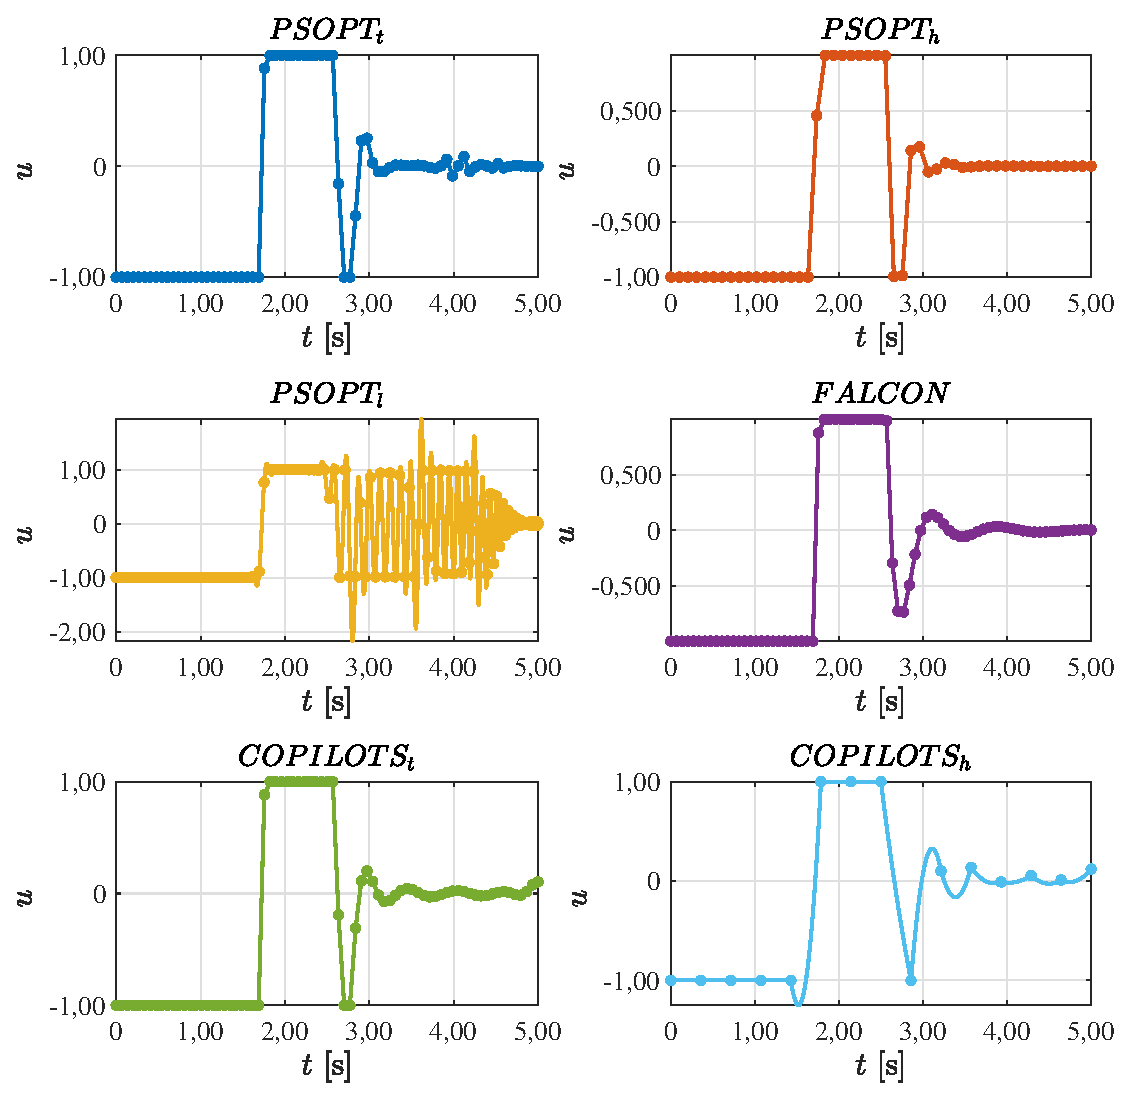
\includegraphics[scale=0.7]{fig/resultados/singular1/traj/u/u}
	\captionof{figure}[Variável de estado $u(t)$ para o problema singular 1]{Variável de estado $u(t)$ para o problema singular 1. Os pontos representam os valores discretizados e as linhas contínuas representam as trajetórias interpoladas.}
	\label{fig:singular1:u:u}
	\vspace{\onelineskip}
\end{minipage}

\noindent
\begin{minipage}{\textwidth}
	\vspace{\onelineskip}
	\centering
	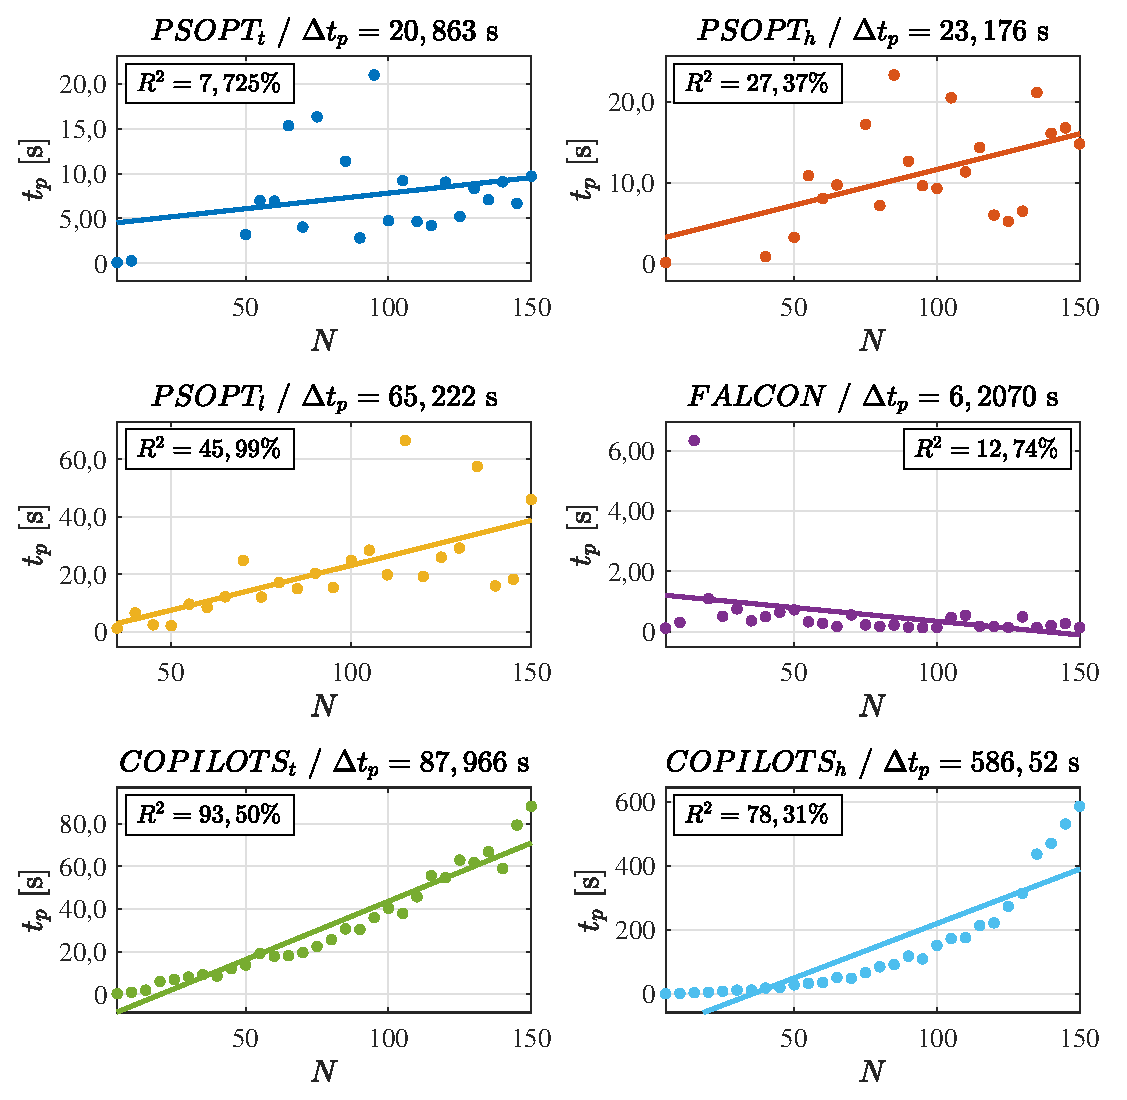
\includegraphics[scale=0.7]{fig/resultados/singular1/sens/t}
	\captionof{figure}[Relação entre o tempo de processamento e o número de nós de colocação para o problema singular 1]{Relação entre o tempo de processamento $ t_p $ e o número de nós de colocação $ N $, considerando cada um dos métodos em análise.}
	\label{fig:singular1:sensibilidade:t}
	\vspace{\onelineskip}
\end{minipage}

\noindent
\begin{minipage}{\textwidth}
	\vspace{\onelineskip}
	\centering
	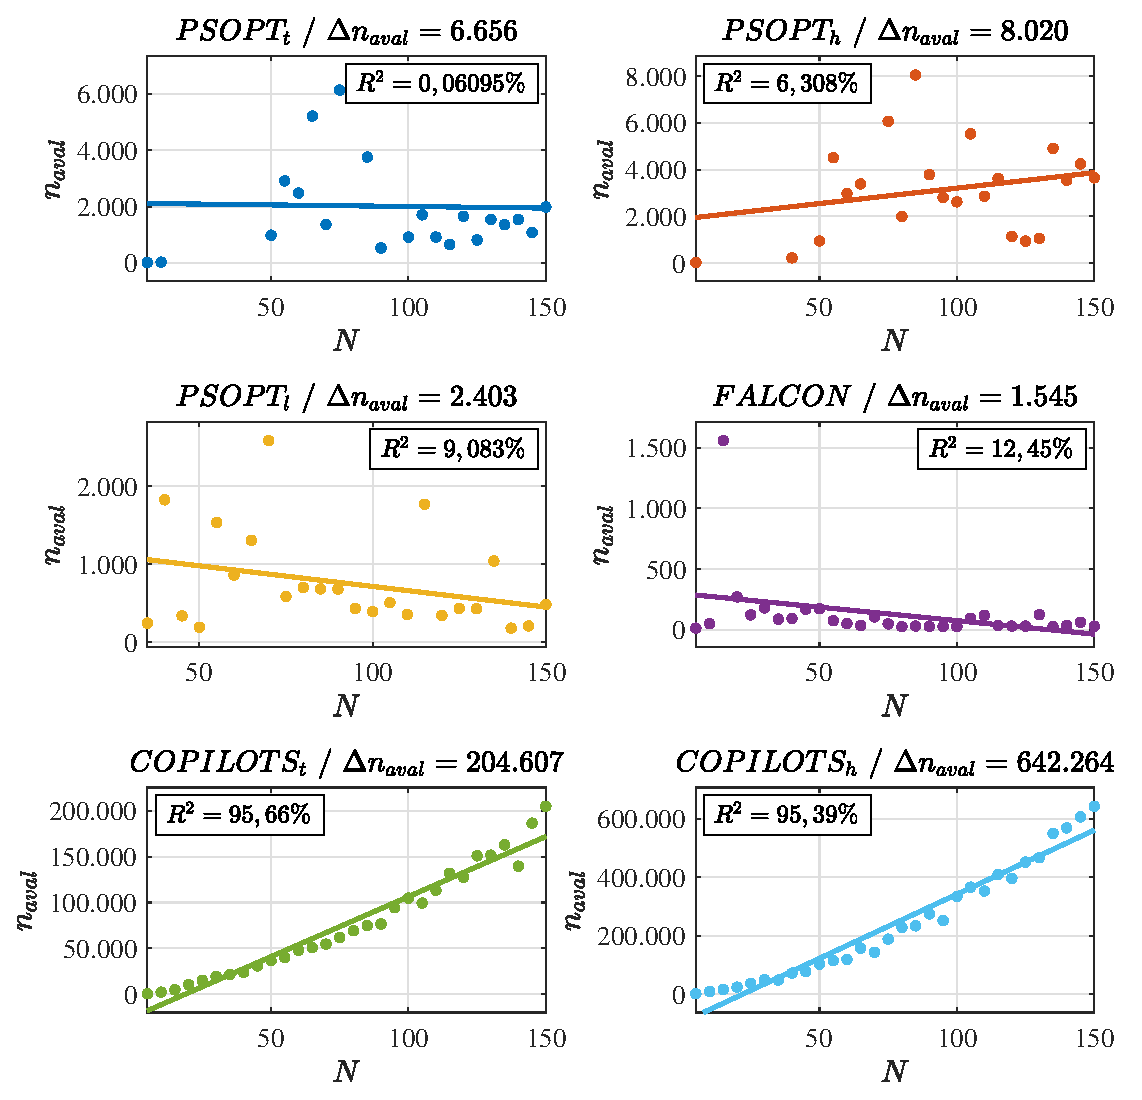
\includegraphics[scale=0.7]{fig/resultados/singular1/sens/eval}
	\captionof{figure}[Relação entre o número de avaliações da função objetivo e o número de nós de colocação para o problema singular 1]{Relação entre o número de avaliações da função objetivo $ n_{aval} $ e o número de nós de colocação $ N $, considerando cada um dos métodos em análise.}
	\label{fig:singular1:sensibilidade:naval}
	\vspace{\onelineskip}
\end{minipage}



% singular2
\subsection{Caso 2}
\label{sec:resultados:singular2}
\label{sec:singular2}

\todo[inline, color=pink]{Função objetivo}

Seja a seguinte função objetivo:
%
\begin{equation}
	\label{eq:singular2:J}
	J = x_3(t_f)
\end{equation}
%
sujeito ao conjunto de equações diferenciais e restrição no controle:
%
\begin{equation}
	\label{eq:singular2:dinamica}
	\begin{gathered}
		\dot{x}_1(t) = x_2(t),\;\;x_1(0) = 0 \\
		\dot{x}_2(t) = u(t),\;\;x_2(0) = 1 \\
		\dot{x}_3(t) = x_1^2(t) + x_2^2(t),\;\;x_3(0) = 0\\
		-1 \leq |u(t)| \leq 1
	\end{gathered}
\end{equation}
%
em que $t$ é o tempo ($t_f$ é o tempo final) e $ \mathbf{x}(t) = \begin{bmatrix} x_1(t) & x_2(t) & x_3(t) \end{bmatrix}^T $ é o vetor de variáveis de estado e $ u(t) $ é a variável de controle. 

Conforme o primeiro estudo de caso singular, a estimativa inicial para o estado e para o controle foi determinada por cada pacote. 

\todo[inline, color=pink]{Introdução da análise de sensibilidade $ J \times N $}

São apresentados na Figura \ref{fig:singular2:sensibilidade:J} a influência do número de nós de colocação no valor da função objetivo (melhor solução encontrada). A faixa considera nesta análise é a mesma empregada para o problema singular 1 (30 pontos igualmente espaçados no intervalo [5 150]).

\noindent	
\begin{minipage}{\textwidth}
	\vspace{\onelineskip}
	\centering
	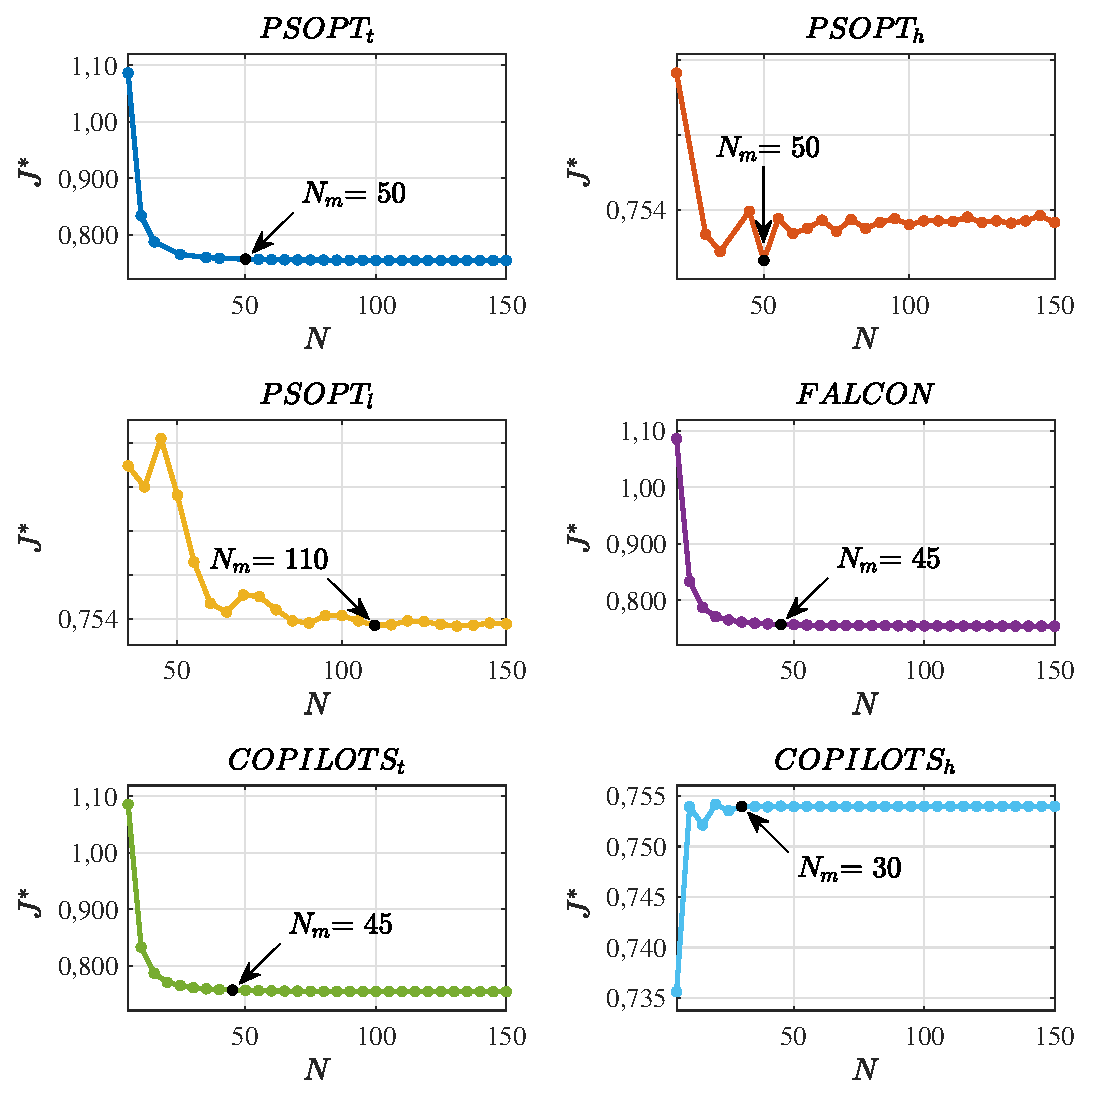
\includegraphics[scale=0.70]{fig/resultados/singular2/sens/J}
	\captionof{figure}[Influência do número de nós de colocação no valor da função objetivo para o problema singular 2]{Influência do número de nós de colocação $ N $ no valor da função objetivo $ J^* $ para o problema singular 2.}
	\label{fig:singular2:sensibilidade:J}
	\vspace{\onelineskip}
\end{minipage}

\todo[inline, color=pink]{Análise dos gráficos $ J \times N $}

De forma geral observa-se que a maioria dos pacotes utilizados, a partir de um determinado valor de $ N_m $, conseguiram convergir para a solução reportada por \textcolor{red}{Arthur, aqui colocar a referência e o valor ótimo para o problema}. O único em que não foi observada uma tendência de convergência ao se aumentar o valor de $N$ foi o $ PSOPT_h$. Para este observa-se um comportamento oscilatório. Assim, o valor de $ N_m $ para esta configuração foi definido como sendo aquele com o menor valor em termos de $ J^* $. Já para o $ COPILOTS_h $ verifica-se um comportamento inesperado, isto é; tanto $ J^* $ quanto $ N $ crescem simultaneamente até que a convergência seja atingida. Tal comportamento pode ser justificado pelo não atendimento das restrições para um número de pontos inferior à, aproximadamente, 30 nós de colocação. Neste caso, por não atender as restrições não considera-se, para $N$ menor que, aproximadamente, 30, que a solução do problema tenha sido obtida. Este resultado inesperado justifica a necessidade de sempre realizar a análise de sensibilidade do problema, bem como avaliar o atendimento das restrições que constituem o mesmo.

\textcolor{red}{Arthur, tentei justificar esse comportamento a partir do não atendimento das restições, mesmo sem saber se é isso. KKKK. Eu imagino que seja isso. O não atendimento pode levar a resultados incoerentes, principalmente no que tange a FO. Por este motivo esta justificativa não é tão groseira ... concorda?}
%sendo 
%%
%\begin{equation}
%J_{N_m} = 0,99 \, \big(max(J^*) - min(J^*)\big) + min(J^*)
%\end{equation}

Além disso, pode ser observada uma boa concordância entre os resultados obtidos por quase todas as abordagens que fazem uso da colocação trapezoidal ($ PSOPT_t $, o $ FALCON $ e o $ COPILOTS_t $). No entanto, observa-se que, empregando o $ PSOPT_t $, não foi possível solucionar o estudo de caso em análise para $ N = 20 $, $ N = 30 $ e $ N = 45 $. Também é possível observar que o valor de $ J^* $ encontrado pelo $ PSOPT_l $ diminui lentamente com o aumento de $ N $ e oscila algumas vezes antes de atingir a convergência. Tal comportamento pode estar associado às propriedades numéricas inerentes à colocação pseudo-espectral, sendo que esta não é a abordagem mais empregada para a  resolução de PCOs com descontinuidades nos controles e/ou estados \cite{becerra_tutorial_2010}. 

Por fim destaca-se que o valor de $ J^* $ referente ao $ PSOPT_h $ se mostrou pouco sensível a variações em $ N $, sendo $ \min(J^*) = 0,753932 $ e $ \max(J^*) = 0,754183$. O mesmo pode ser observado para o $ PSOPT_l $, sendo nesse caso $ \min(J^*) = 0,753984 $ e $\max(J^*) = 0,754411$. 

\todo[inline, color=pink]{Introdução dos resultados $ N = N_m $}

A  Tabela \ref{tab:singular2:raw} apresenta um resumo das métricas obtidas por cada pacote. Neste destacam-se o valor da função objetivo ($ J^* $), o tempo de processamento médio ($ t_p $), o desvio padrão atribuído ($ s_t $), a máxima violação das restrições ($ \Delta c_{max} $) e o número de execuções bem sucedidas ($ N_s $).

\begin{table}[!h]
	\centering
	\caption[Métricas obtidas para o problema singular 2]{Métricas obtidas para o problema singular 2. Os melhores $ N_m $, $ J^* $, $ t_p $, $ n_{aval} $ e $ N_s\% $ se encontram destacados.}
	\label{tab:singular2:raw}
	\begin{tabular}{ccccccccc}
		\hline
		Método       & $N_m$                              & $J^*$                                   & $t_p$ {[}$s${]}                         & $s_t$ {[}$s${]} & $n_{aval}$                         & $\Delta c_{max}$                & $N_s$ & $N_s\%$                                  \\ \hline
		$PSOPT_t$    & 50                                 & 0,75663                                 & 3,20295                                 & 0,08123         & 924                                & 3,12e-11                        & 27    & 90,00\%                                  \\
		$PSOPT_h$    & 50                                 & {\color[HTML]{009901} \textbf{0,75393}} & 3,50511                                 & 0,08317         & 1060                               & 4,16e-09                        & 25    & 83,33\%                                  \\
		$PSOPT_l$    & 110                                & 0,75399                                 & 15,91228                                & 0,16007         & 214                                & 1,16e-07                        & 24    & 80,00\%                                  \\
		$FALCON$     & 45                                 & 0,75720                                 & {\color[HTML]{009901} \textbf{0,37631}} & 0,04386         & {\color[HTML]{009901} \textbf{76}} & 2,36e-09                        & 30    & {\color[HTML]{009901} \textbf{100,00\%}} \\
		$COPILOTS_t$ & 45                                 & 0,75720                                 & 17,77565                                & 0,37422         & 37149                              & 3,32e-12                        & 30    & {\color[HTML]{009901} \textbf{100,00\%}} \\
		$COPILOTS_h$ & {\color[HTML]{009901} \textbf{30}} & 0,75397                                 & 34,27460                                & 0,41814         & 105399                             & {\color[HTML]{000000} 1,63e-12} & 30    & {\color[HTML]{009901} \textbf{100,00\%}} \\ \hline
	\end{tabular}
\end{table}

\todo[inline, color=pink]{Análise dos resultados $ N = N_m $}

Nesta tabela, os valores de $ J^* $ associados ao $ PSOPT_h $ e ao $ COPILOTS_h $ se mostram bastante próximos, sendo o $ J^* $ atribuído ao $ PSOPT_h $ o menor dentre os obtidos. Em relação ao $ FALCON $ e ao $ COPILOTS $, associam-se os menores $ N_m $. Além disso, observa-se no $ COPILOTS_h $ o menor valor em termos de $ N_m $. Em geral, os $ N_m $ associados aos métodos que fazem uso da colocação trapezoidal são maiores que os requeridos pelos que empregam a colocação de  Hermite-Simson. De fato, essa tendência é observada quando comparam-se os valores de $ N_m $ do $ COPILOTS_t $ e do $ COPILOTS_h $. No entanto, não se verifica esse mesmo comportamento quando avaliam-se os $ N_m $ associados ao $ PSOPT_t $ e ao $ PSOPT_h $. Esse resultado pode estar relacionado ao tipo de otimizador considerado pelo  $ PSOPT $, isto é. ao Método de Ponto Interior \cite{wachter_implementation_2006}.

Ao se empregar o $ FALCON $ observa-se os menores valores para $ t_p $ e para $ n_{aval} $. Em contrapartida, ao $ COPILOTS $ estão associados os maiores $ t_p $ e $ n_{aval} $. Provavelmente, esta diferença se deve as características de cada pacote, bem como ao uso de informações simbólicas empregadas pelo $ FALCON $. Foi somente empregando o $ COPILOTS $ e o $ FALCON $ que este estudo de caso foi resolvido para os valores de $N$ adotados. Por outro lado, o menor valor de $ N\% $ e o maior valor de $ N_m $ foi obtido pelo $ PSOPT_l $. Esses resultados indicam que a colocação pseudo-espectral não deve ser empregada na resolução de PCOs aos quais estejam associadas descontinuidades nos controles e/ou estados \cite{becerra_tutorial_2010}. 

É importante ressaltar que em relação ao $ PSOPT $, o maior valor de $ t_p $ foi encontrado para a configuração pseudo-espectral. Esse resultado indica que nem sempre há uma relação direta entre $ t_p $ e $ n_{aval} $, e que a associação entre essas variáveis depende do método empregado na resolução do estudo de caso em análise. 

\todo[inline, color=pink]{Introdução das trajetórias}

As trajetórias obtidas para o vetor de variáveis de estado e controle são apresentadas nas Figuras \ref{fig:singular2:x:x1}-\ref{fig:singular2:u:u} considerando $N$ igual a $N_m$. Ao se analisar os resultados pode-se perceber a similaridade entre todos os perfis referentes as variáveis de estado. Em relação ao controle, observa-se uma mesma tendência, todavia são observadas oscilações na maiores dos pacotes. As trajetórias de controle associadas ao $ PSOPT_t $ e ao $ PSOPT_h $ se mostraram oscilatórias, o que pode ser devido ao otimizador considerado. Já aquelas associadas aos demais métodos apresentaram apenas leves oscilações após a primeira variação abrupta de $ u(t) $, que ocorre em $ t \approx 1,3 $ s. No caso do $ PSOPT_l $ foram observadas leves oscilações ao fim da trajetória, o que se deve ao alto valor de $ N_m $ empregado. Em contrapartida, o $ FALCON $ apresenta uma trajetória mais suave em relação as outras abordagens empregadas. 

A influência do número de nós de colocação no tempo de processamento e no número de avaliações da função objetivo são apresentadas nas Figuras \ref{fig:singular2:sensibilidade:t} e \ref{fig:singular2:sensibilidade:naval}. Nestes gráficos são apresentadas as variações: $ \Delta t_p = \max\{t_p\} - \min\{t_p\} $ e $ \Delta n_{aval} = \max\{n_{aval}\} - \min\{n_{aval}\} $. Os pontos nos gráficos representam os valores atribuídos a $ t_p $ (e a $ n_{aval} $) para cada um dos $ N $ considerados, enquanto as linhas contínuas representam curvas de tendência, obtidas por meio de regressões lineares, em que $R^2$ é o coeficiente de determinação. Os valores de $ N $ empregados na geração desses resultados são iguais àqueles considerados na computação da relação entre $ J^* $ e $ N $. 

\noindent
\begin{minipage}{\textwidth}
	\vspace{\onelineskip}
	\centering
	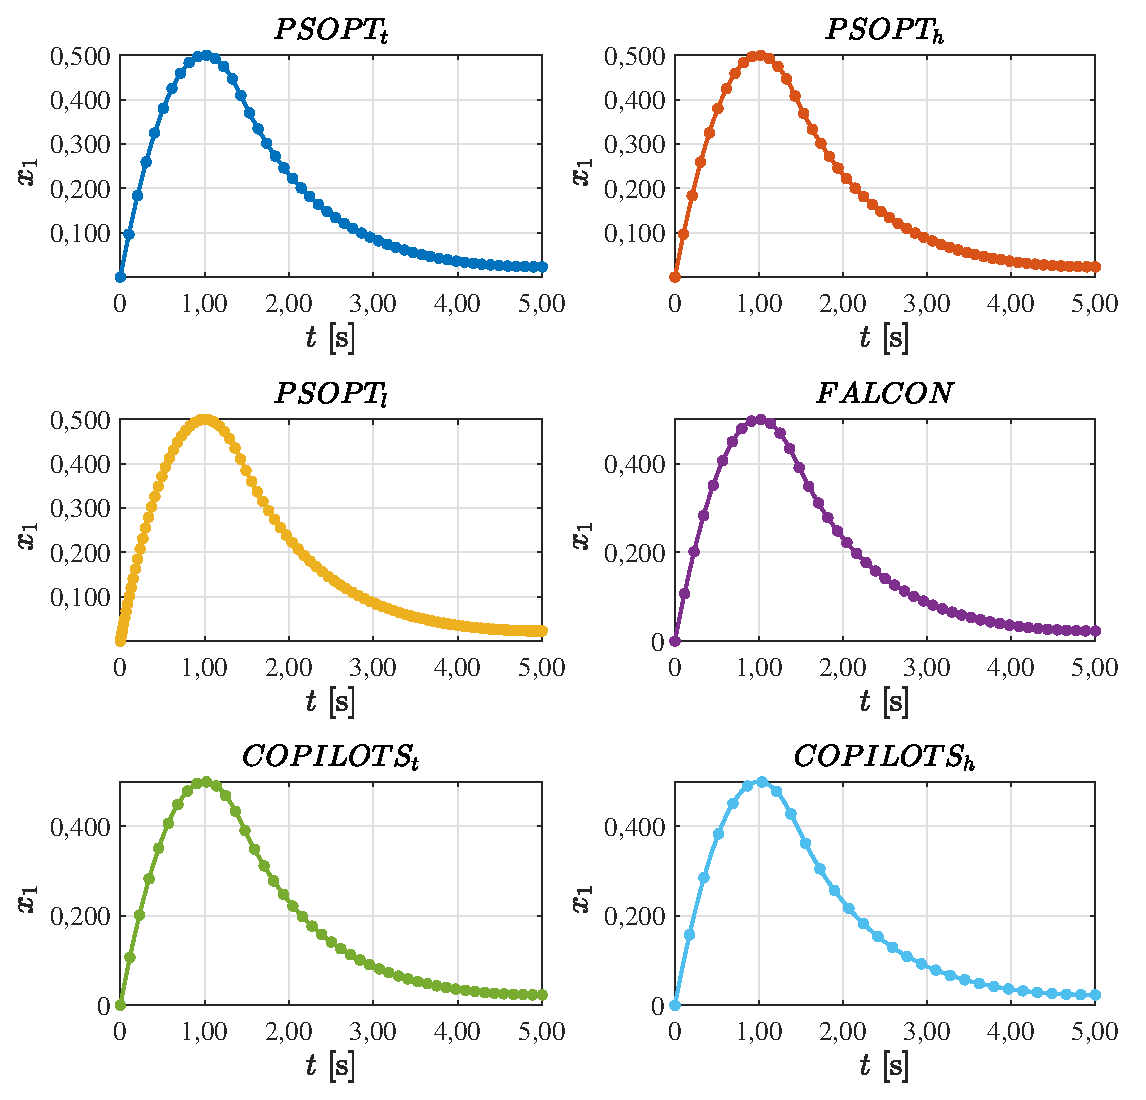
\includegraphics[scale=0.70]{fig/resultados/singular2/traj/x/x_1}
	\captionof{figure}[	Variável de estado $x_1(t)$ para o problema singular 2]{Variável de estado $x_1(t)$ para o problema singular 2. Os pontos representam os valores discretizados e as linhas contínuas representam as trajetórias interpoladas.}
	\label{fig:singular2:x:x1}
	\vspace{\onelineskip}
\end{minipage}

\noindent
\begin{minipage}{\textwidth}
	\vspace{\onelineskip}
	\centering
	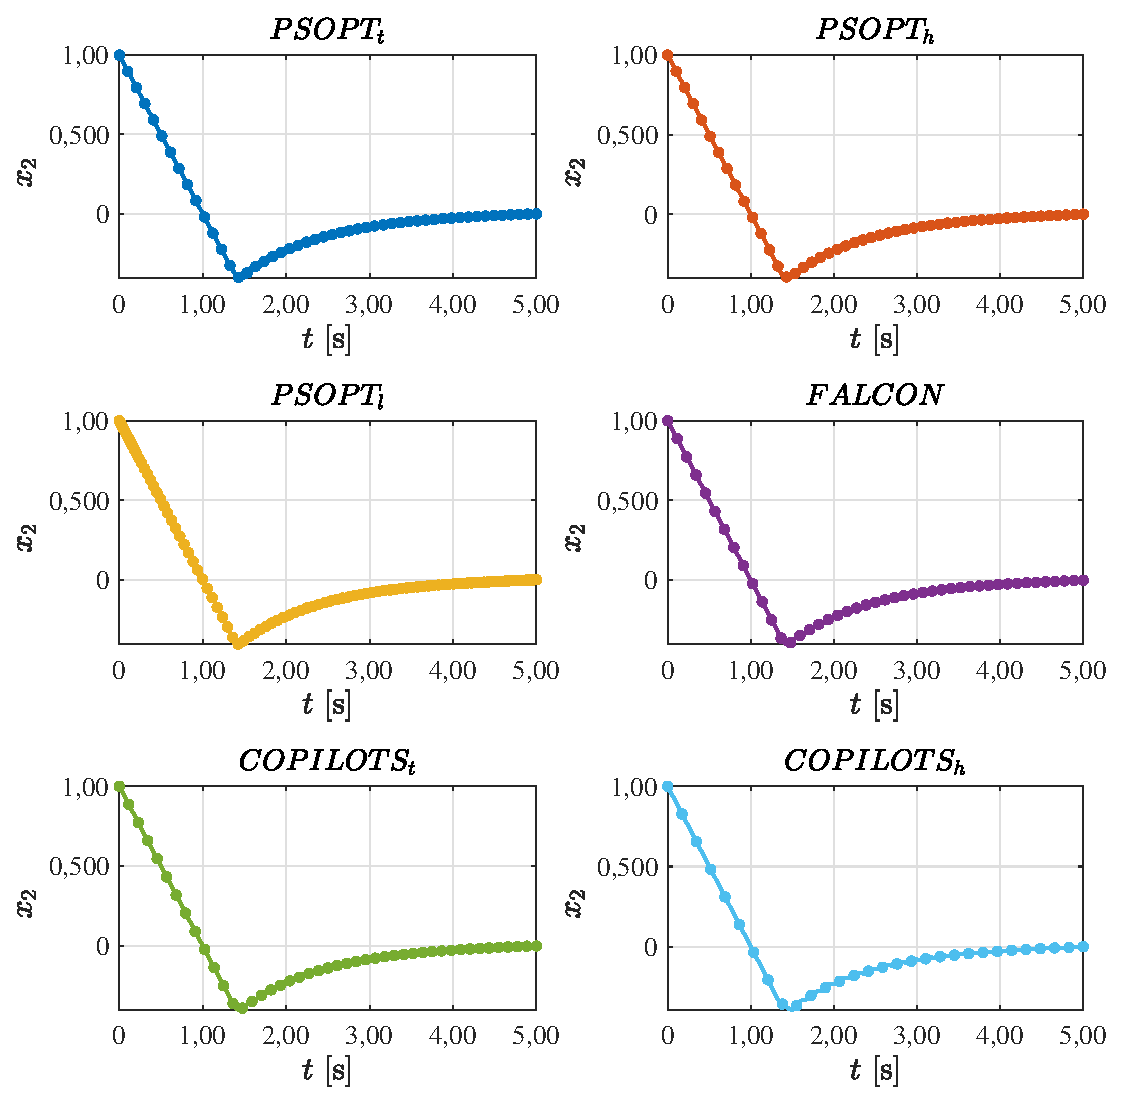
\includegraphics[scale=0.70]{fig/resultados/singular2/traj/x/x_2}
	\captionof{figure}[Variável de estado $x_2(t)$ para o problema singular 2]{Variável de estado $x_2(t)$ para o problema singular 2. Os pontos representam os valores discretizados e as linhas contínuas representam as trajetórias interpoladas.}
	\label{fig:singular2:x:x2}
	\vspace{\onelineskip}
\end{minipage}

\noindent
\begin{minipage}{\textwidth}
	\vspace{\onelineskip}
	\centering
	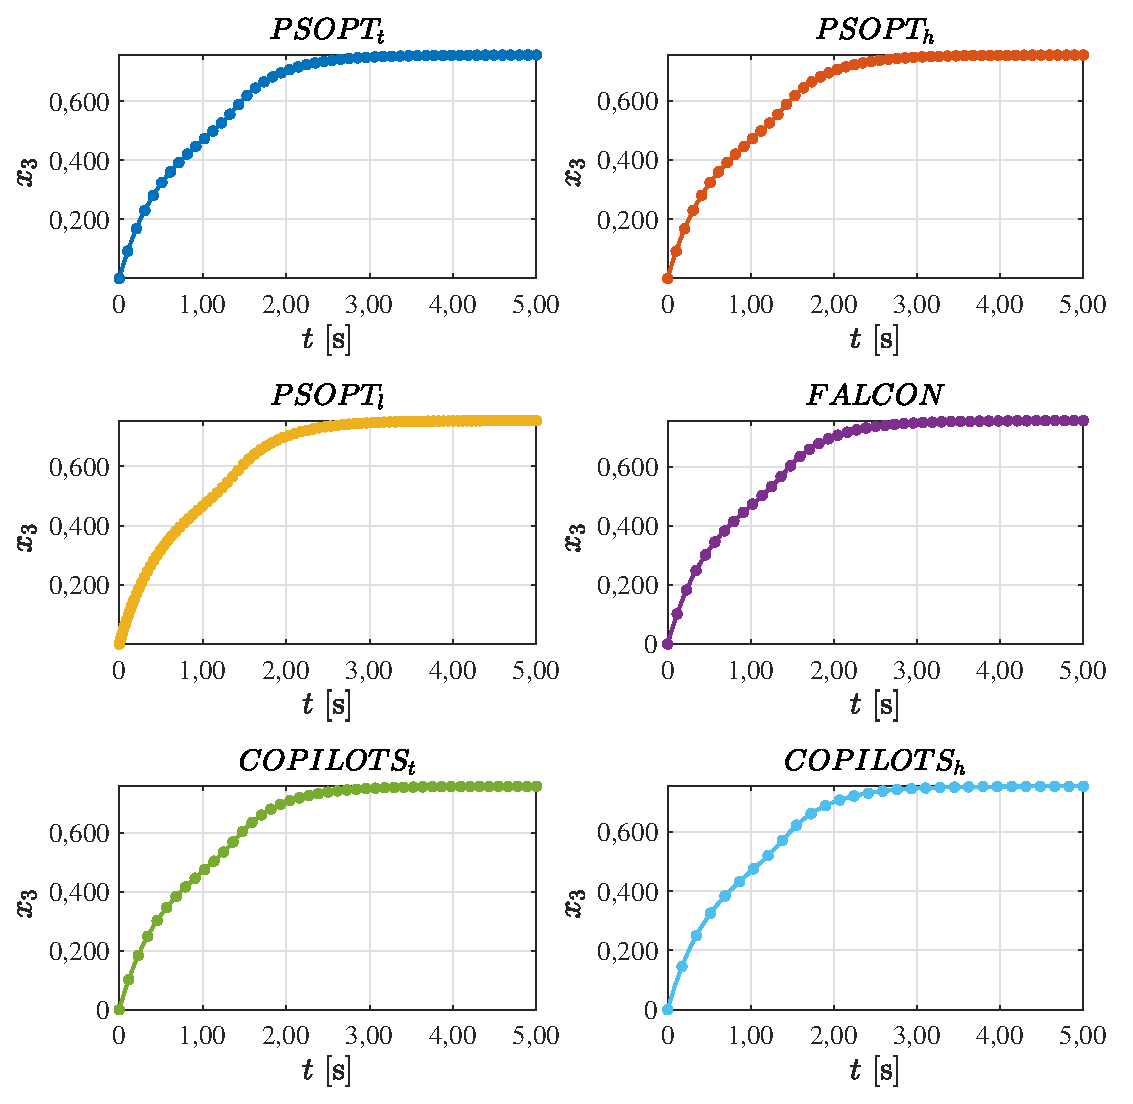
\includegraphics[scale=0.70]{fig/resultados/singular2/traj/x/x_3}
	\captionof{figure}[Variável de estado $x_3(t)$ para o problema singular 2]{Variável de estado $x_3(t)$ para o problema singular 2. Os pontos representam os valores discretizados e as linhas contínuas representam as trajetórias interpoladas.}
	\label{fig:singular2:x:x3}
	\vspace{\onelineskip}
\end{minipage}

\noindent
\begin{minipage}{\textwidth}
	\vspace{\onelineskip}
	\centering
	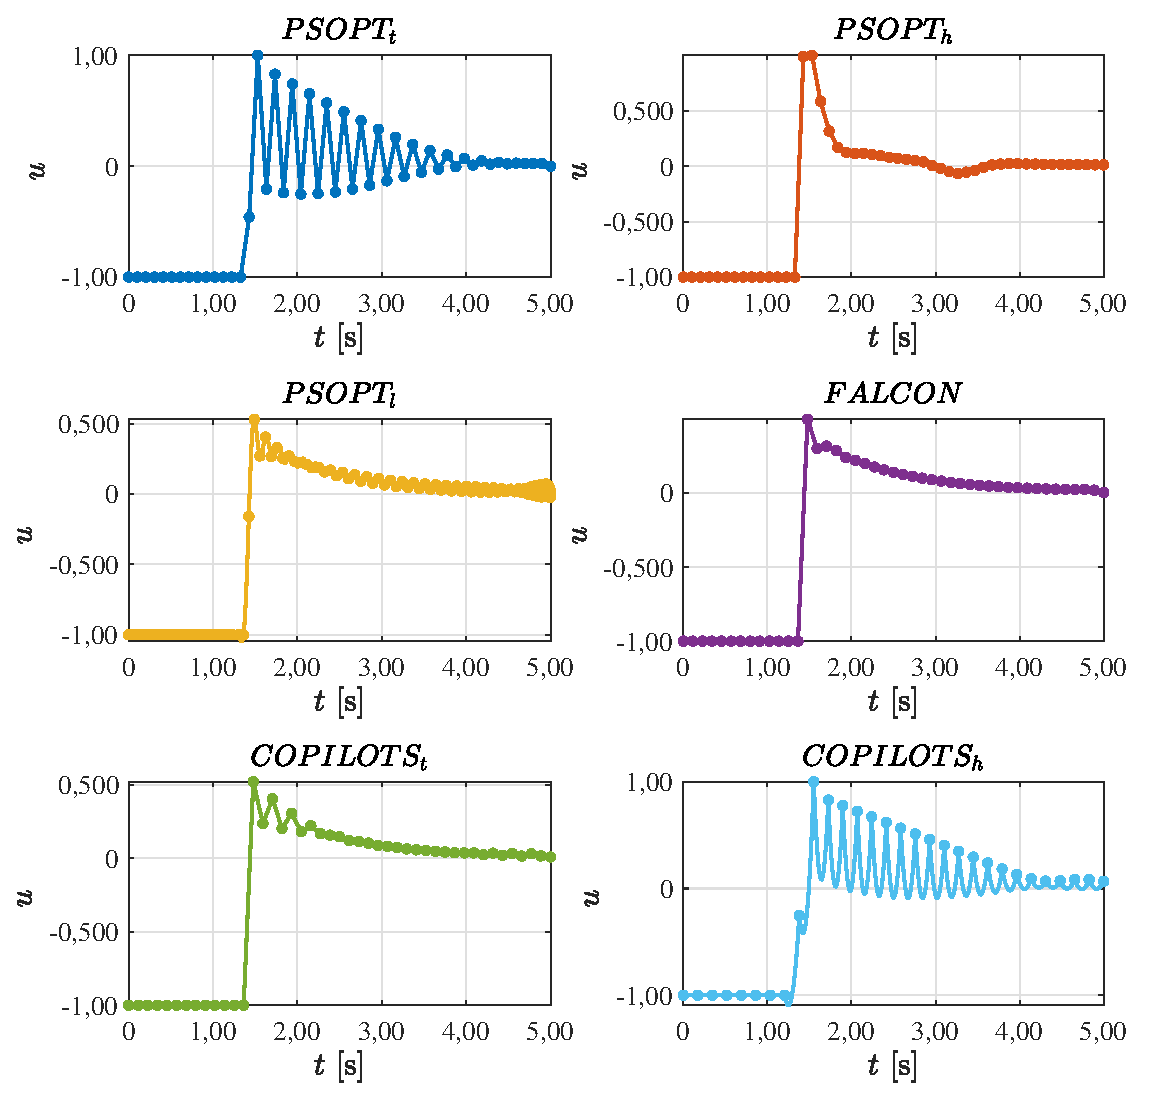
\includegraphics[scale=0.70]{fig/resultados/singular2/traj/u/u}
	\captionof{figure}[Variável de controle $u(t)$ para o problema singular 2]{Variável de controle $u(t)$ para o problema singular 2. Os pontos representam os valores discretizados e as linhas contínuas representam as trajetórias interpoladas.}
	\label{fig:singular2:u:u}
	\vspace{\onelineskip}
\end{minipage}

\todo[inline, color=pink]{Análise das trajetórias}


\todo[inline, color=pink]{Introdução dos resultados $ t_p \times N $ e $ n_{aval} \times N $}

\noindent
\begin{minipage}{\textwidth}
	\vspace{\onelineskip}
	\centering
	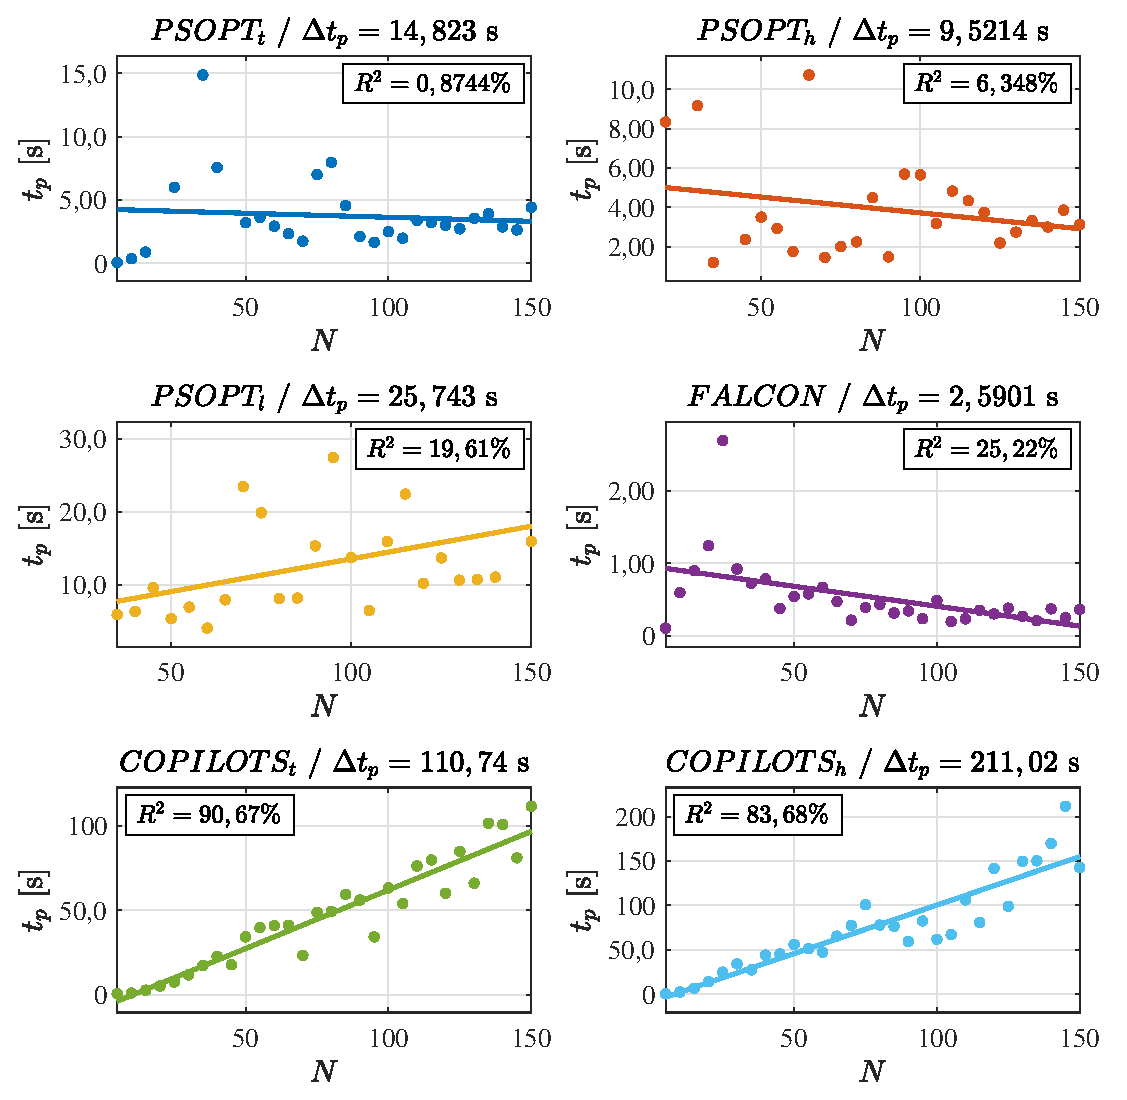
\includegraphics[scale=0.70]{fig/resultados/singular2/sens/t}
	\captionof{figure}[Relação entre o tempo de processamento e o número de nós de colocação para o problema singular 2]{Relação entre o tempo de processamento $ t_p $ e o número de nós de colocação $ N $, considerando cada um dos métodos em análise.}
	\label{fig:singular2:sensibilidade:t}
	\vspace{\onelineskip}
\end{minipage}

Nas Figuras \ref{fig:singular2:sensibilidade:t} e \ref{fig:singular2:sensibilidade:naval} observa-se que os valores de $ t_p $ e de $ n_{aval} $ associados ao $ FALCON $ se mostraram pouco sensíveis a variações em $ N $, dados os baixos $ \Delta t_p $ e $ \Delta n_{aval} $ associados a esse pacote. Em relação ao $ PSOPT$, a configuração pseudo-espectral foi a que resultou em um maior tempo de processamento. Esse comportamento se deve às características numéricas inerentes à colocação pseudo-espectral, que não deve ser empregada na solução de PCOs aos quais estejam associadas descontinuidades nos controles \cite{becerra_tutorial_2010}. Em contrapartida, o $ n_{aval} $ vinculado ao $ PSOPT_l $ se mostrou menos sensível a variações em $ N $ que aqueles associados ao $ PSOPT_t $ e ao $ PSOPT_h $. 

Os métodos associados ao $ COPILOTS $ se mostraram bastante sensíveis a variações em $ N $, com $ \Delta t_p $ e $ \Delta n_{aval} $ consideravelmente mais altos que os atribuídos aos demais métodos. Esse comportamento se deve ao uso que o pacote faz do SQP utilzado. Com o aumento de $ N $, os valores de $ t_p $ e de $ n_{aval} $ associados ao $ PSOPT_t $, $ PSOPT_h $ e $ FALCON $, e os valores de $ n_{aval} $ requeridos pelo $ PSOPT_l $ tendem a convergir. Além disso, nota-se que os valores de $ t_p $ e de $ n_{aval} $ diminuem à medida que alcançam essa convergência para algumas configurações utilizadas, comportamento oposto àquele que espera-se observar nesses casos. A presença de picos nos $ t_p $ e $ n_{aval} $ observados em cada um desses métodos ajuda a explicar este comportamento anômalo. Em resumo, devido à presença de alguns picos existe uma falsa impressão que o aumento no valor de $N$ implica na redução do tempo de processamento (ver a Figura \ref{fig:singular2:sensibilidade:t}). Este mesmo comportamento pode ser observado na Figura \ref{fig:singular2:sensibilidade:naval} para todas as configurações $ PSOPT$ e do $FALCON $. Neste caso, menores valores de $N$ podem resultar em um menor número de avaliações da função objetivo, porém, a convergência acontece para um valor que não é a solução do problema, conforme observado na Figura \ref{fig:singular2:sensibilidade:J}. Já para todas as versões do $ COPILOTS $ são observados perfis mais próximos aos esperados para $ t_p $ e de $ n_{aval} $, isto é; o aumento no valor de $N$ implica no aumento destes dois parâmetros, conforme observado nas Figuras \ref{fig:singular2:sensibilidade:t}) e  \ref{fig:singular2:sensibilidade:naval}.

\noindent
\begin{minipage}{\textwidth}
	\vspace{\onelineskip}
	\centering
	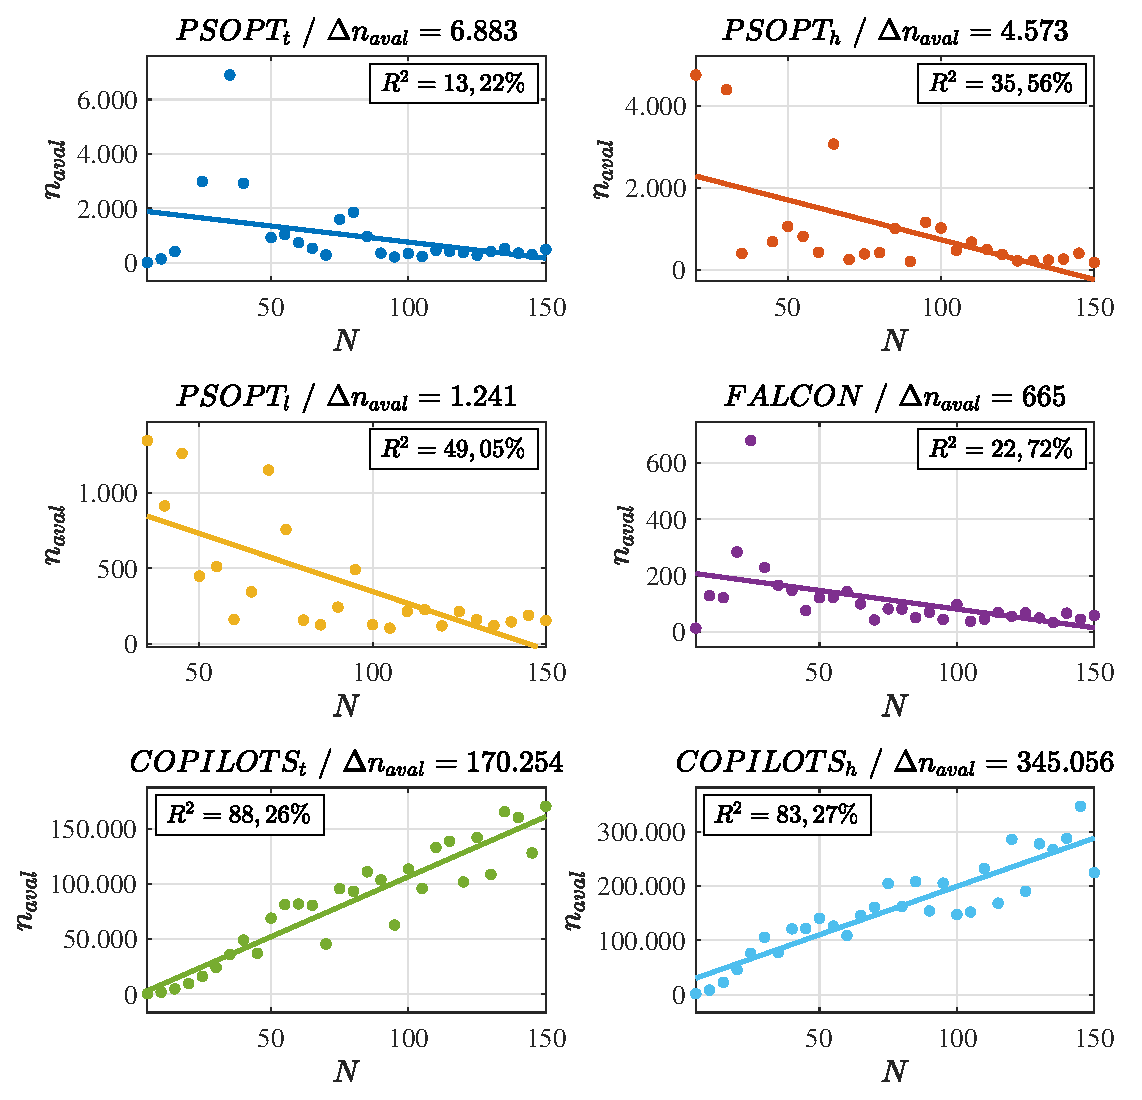
\includegraphics[scale=0.70]{fig/resultados/singular2/sens/eval}
	\captionof{figure}[Relação entre o número de avaliações da função objetivo e o número de nós de colocação para o problema singular 2]{Relação entre o número de avaliações da função objetivo $ n_{aval} $ e o número de nós de colocação $ N $, considerando cada um dos métodos em análise.}
	\label{fig:singular2:sensibilidade:naval}
	\vspace{\onelineskip}
\end{minipage}

\todo[inline, color=pink]{Análise dos resultados $ t_p \times N $ e $ n_{aval} \times N $}



% penduloInvertido
\section{Minimização do esforço durante o \textit{Swing-up} de um pêndulo invertido}
\label{sec:resultados:penduloInvertido}
\todo[inline, color=pink, size=normalsize]{Introdução da seção}

O pêndulo invertido é um sistema comumente empregado no ensino da teoria do Controle de Sistemas \cite{kelly_introduction_2017}. No entanto, a dinâmica associada ao pêndulo invertido pode ser empregada na modelagem da caminhada de robôs humanoides \cite{venancio_desenvolvimento_2018}, no estudo da dinâmica de foguetes durante o lançamento \cite{peltroche_advanced_2019}, e no controle de veículos do tipo \textit{Segway}\textsuperscript{\textregistered} \cite{younis_design_2009}.  

Para fins de aplicação considere o pêndulo invertido apresentado na Figura \ref{fig:penduloInvertido:variaveis}. Este é composto por um carro que, impulsionado por um motor, se move ao longo de um trilho e por um pêndulo que pende livremente desse carro. O ângulo entre o pêndulo e a vertical é dado por $ \theta(t) $, enquanto $ \omega(t) $ e $ l $ são a velocidade angular do pêndulo e o comprimento de sua haste. A distância entre o carro e o centro do trilho é dada por $ d(t) $, enquanto $ v(t) $ é a velocidade do carro, $ F(t) $ é a força que o impulsiona, $ m_1 $ e $ m_2 $ são as massas do carro e do pêndulo, respectivamente, e $ g $ é a aceleração da gravidade \cite{kelly_introduction_2017}.

\noindent	
\begin{minipage}{\textwidth}
	\vspace{\onelineskip}
	\centering
	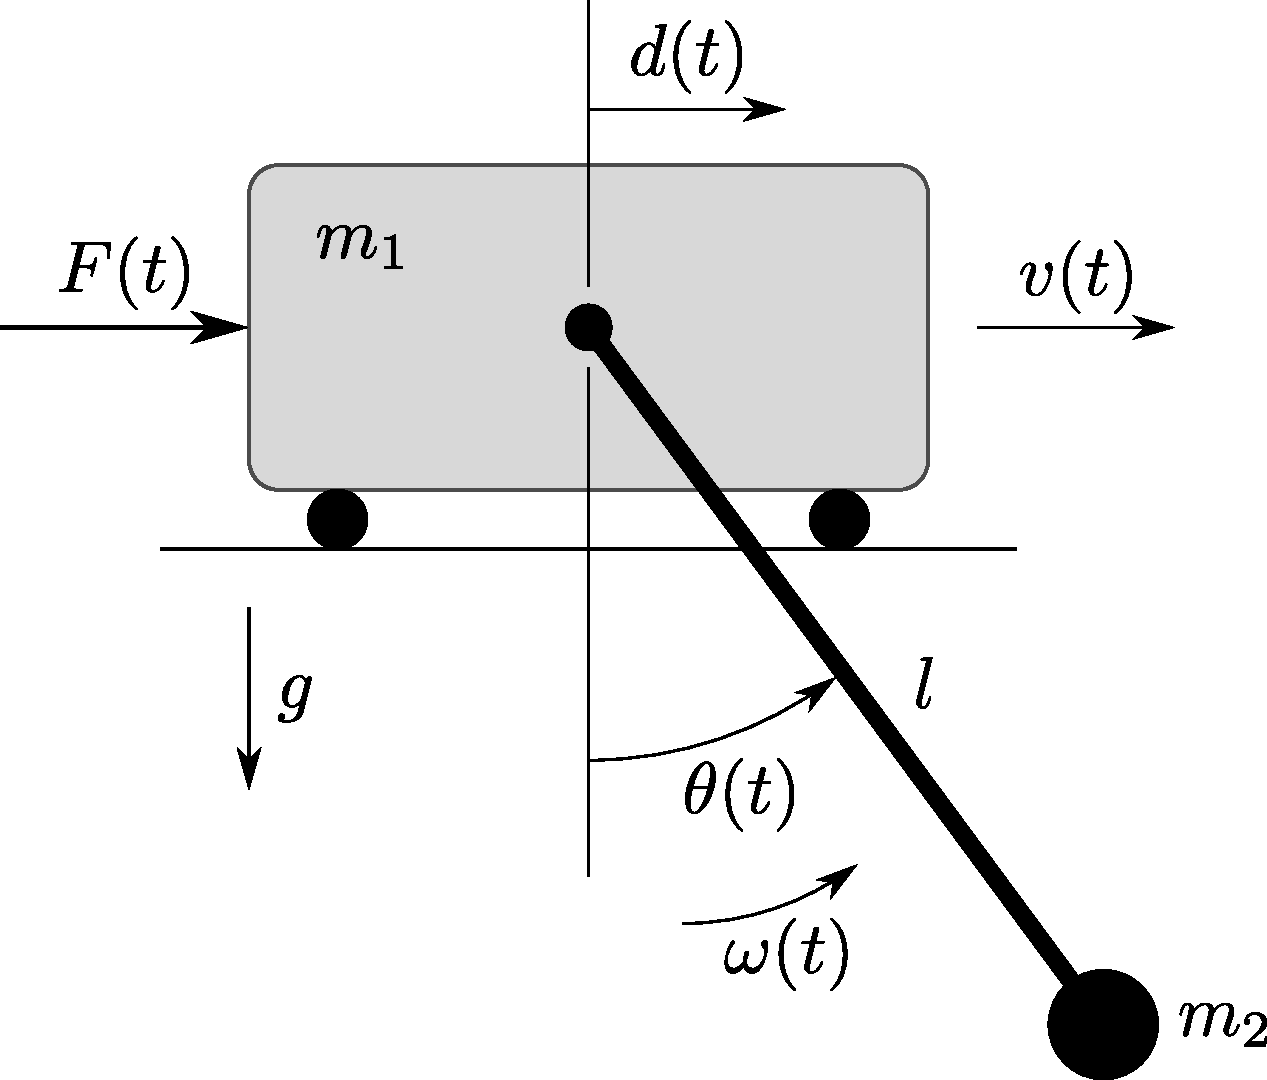
\includegraphics[scale=0.3]{draw/resultados/pdf/pendulo}
	\captionof{figure}[Representação esquemática de um pêndulo invertido]{Representação esquemática de um pêndulo invertido e das variáveis utilizadas na descrição da dinâmica desse sistema.}
	\label{fig:penduloInvertido:variaveis}
	\vspace{\onelineskip}
\end{minipage}

Neste estudo deseja-se determinar a trajetória a ser percorrida pelo um pêndulo invertido para que o mesmo realize uma manobra de balanço ascendente (\textit{swing-up}), empregando o mínimo esforço. Inicialmente em repouso, o carro deve partir do centro do trilho, com a haste do pêndulo pendendo na vertical, e se movimentar de forma que a posição $ d_f $ seja atingida $ t_f $ segundos após o início da manobra, ao mesmo tempo em que a haste do pêndulo, apontando agora para cima, atinge a posição vertical, conforme ilustrado na Figura \ref{fig:penduloInvertido:penduloInicialFinal} \cite{kelly_introduction_2017}. 

\noindent	
\begin{minipage}{\textwidth}
	\vspace{\onelineskip}
	\centering
	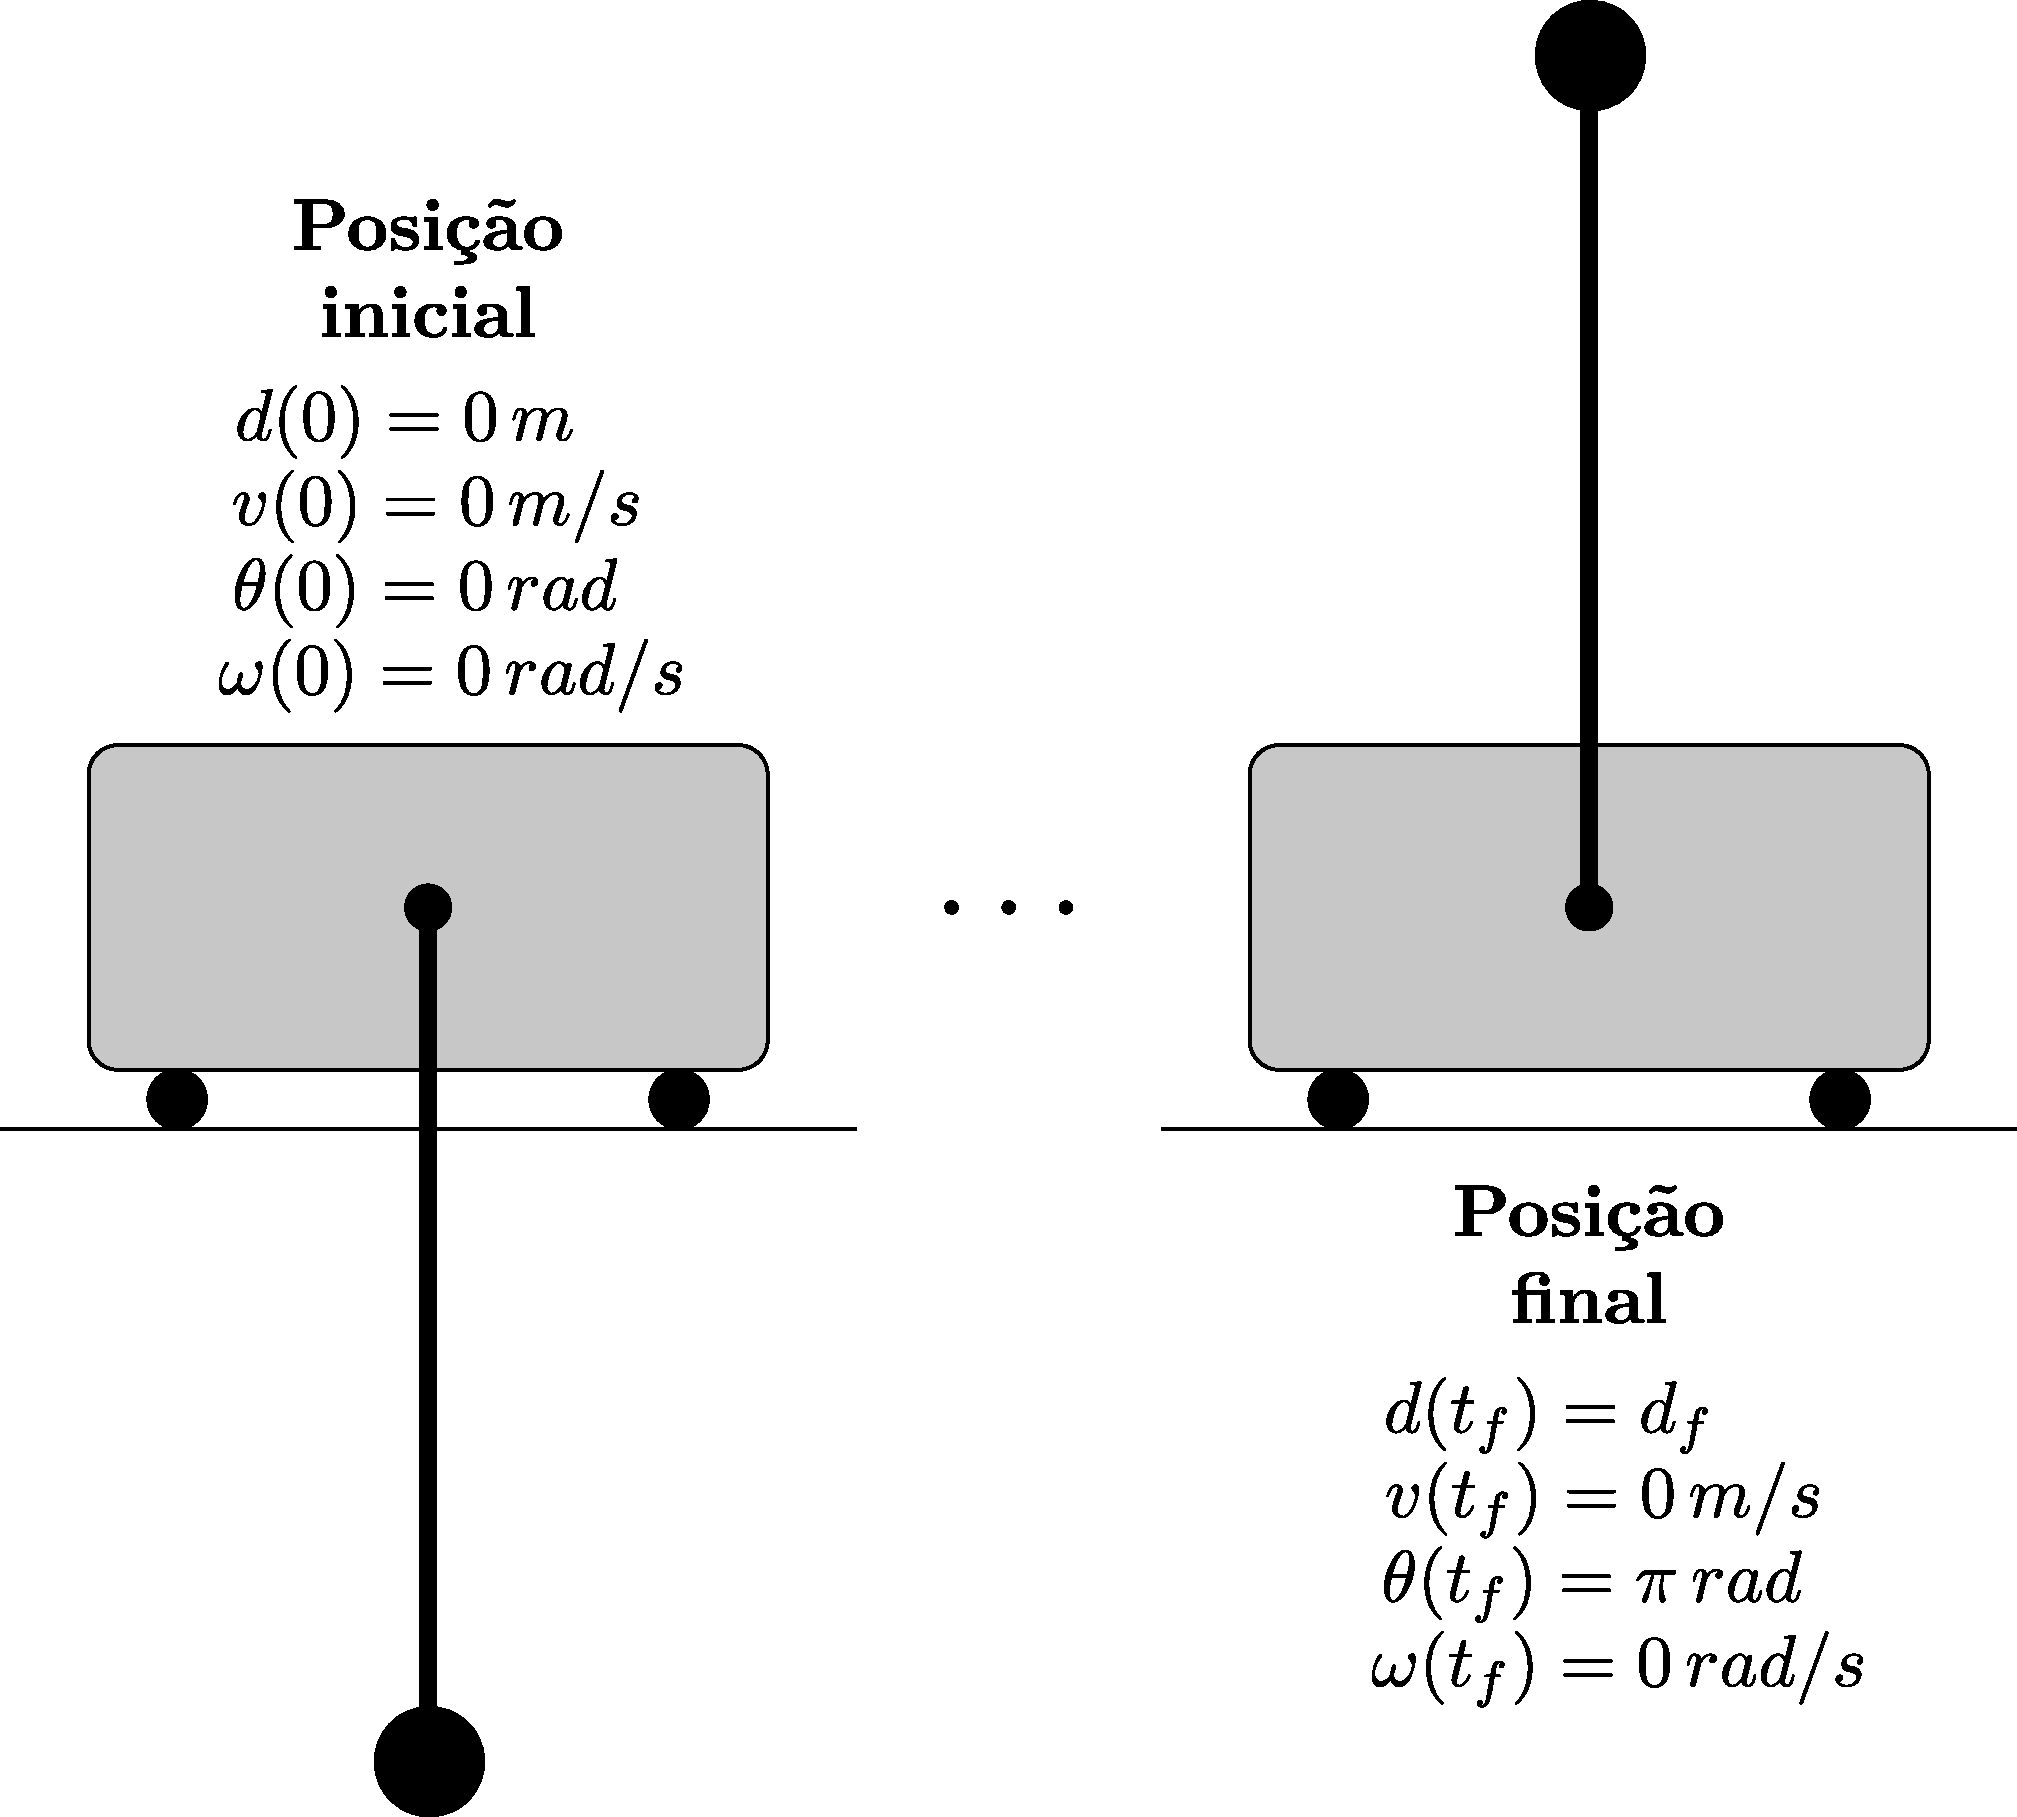
\includegraphics[scale=0.3]{draw/resultados/pdf/penduloInicialFinal}
	\captionof{figure}[Posições inicial e final definidas pra o problema do pêndulo invertido]{Posições inicial e final definidas para o problema do pêndulo invertido durante a execução da manobra de \textit{swing-up}.}
	\label{fig:penduloInvertido:penduloInicialFinal}
	\vspace{\onelineskip}
\end{minipage}

\todo[inline, color=pink, size=normalsize]{Função objetivo}

Para este estudo de caso deseja-se minimizar a função objetivo descrita como \cite{kelly_introduction_2017}:
%
\begin{equation}
	\label{eq:penduloInvertido:J}
	J = \int_{0}^{t_f} F^2(t) dt
\end{equation}
%
sujeito as seguintes restrições:
%
\begin{subequations}
\begin{equation}
\label{eq:penduloInvertido:dinamica}
\dot{d}(t) = v(t),\;\;d(0) = 0 \; \text{m}
\end{equation}
\vspace{-0.75cm}
\begin{equation}
\dot{\theta}(t) = \omega(t),\;\;\theta(0) = 0 \; \text{rad}
\end{equation}
\vspace{-0.75cm}
\begin{equation}
\dot{v}(t) = \frac{l \, m_2 \, \omega^2(t) \, sen \big(\theta(t)\big) + F(t) + m_2 \, g \, cos \big(\theta(t)\big) \, sen\big(\theta(t)\big)}{m_1 + m_2 \big[1 - cos^2 \big(\theta(t) \big)\big]},\;\;v(0) = 0 \; \text{m/s} 
\end{equation}
\vspace{-0.6cm}
\begin{equation}
\dot{\omega}(t) = -\frac{l \, m_2 \, \omega^2(t) \, sen\big(\theta(t)\big) \, cos\big(\theta(t)\big) + F(t) \, cos\big( \theta(t) \big) + (m_1 + m_2) g \, sen\big(\theta(t)\big)}{l \, m_1 + l \, m_2 \big[1 - cos^2\big(\theta(t)\big) \big]},\nonumber
\end{equation}
\vspace{-0.6cm}
\begin{equation}
\omega(0) = 0 \, \text{rad/s}
\end{equation}
\end{subequations}
%
em que $ \mathbf{x}(t) = \begin{bmatrix} d(t) & \theta(t) & v(t) & \omega(t) \end{bmatrix}^T $ é o vetor de variáveis de estados e $ F(t) $ é a variável de controle. 

Uma vez que o trilho sobre o qual o carro se movimenta é finito e levando em conta que há um limite associado à força que o motor pode impor sobre o carro, devem-se considerar as restrições:
%
\begin{subequations}
\begin{equation}
\label{eq:penduloInvertido:laterais}
-d_{max} \leq d(t) \leq d_{max}
\end{equation}
\vspace{-0.5cm}
\begin{equation}
-F_{max} \leq F(t) \leq F_{max}
\end{equation}
\end{subequations}
%
sendo $ d_{max} $ a metade da extensão do trilho e $ F_{max} $ a máxima força que pode ser imposta pelo motor. 

Também são impostas restrições terminais, definidas como segue:
%
\begin{subequations}
\begin{equation}
\label{eq:penduloInvertido:terminais}
d(t_f) = d_f\; \text{m}
\end{equation}
\vspace{-0.85cm}
\begin{equation}
\theta(t_f) = \theta_f\; \text{rad}
\end{equation}
\vspace{-0.7cm}
\begin{equation}
v(t_f) = 0\; \text{m/s}
\end{equation}
\vspace{-0.75cm}
\begin{equation}
\omega(t_f) = 0\;\text{rad/s}
\end{equation}
\end{subequations}

Os parâmetros empregados neste estudo de caso são \cite{kelly_introduction_2017}: aceleração da gravidade ($ g = 9,81 $ m/s$^2$), massa do carro ($ m_1 = 1$ kg), massa do pêndulo ($ m_2 = 0,3 $ kg), comprimento da haste do pêndulo ($ l = 0,5 $ m), tempo final ($ t_f = 2 $ s), distância percorrida pelo carro ao longo da execução da manobra ($ d_f = 1 $ m), posição angular final do pêndulo ($ \theta_f = \pi $ rad), máxima força que pode ser imposta pelo motor que impulsiona o carro ($ F_{max} = 20 $ N), e metade do comprimento do trilho sobre o qual o carro se movimenta ($ d_{max} = 2 $ m).

\todo[inline, color=pink, size=normalsize]{Observações sobre a inicialização dos estados e controles}

Para que as trajetórias das variáveis de estado e de controle obtidas pela metodologia proposta se assemelhem à aquelas reportadas em \citeonline{kelly_introduction_2017}, assume-se, \textit{a priori}, que os estados do sistema evoluem linearmente ao longo da execução da manobra de \textit{swing-up} e que $ F(t) $ permanece nulo para $ t \in [0, \, t_f] $. Assim sendo, para resolução do estudo de caso em análise por meio do $ COPILOTS $ adotou-se as seguintes estimativas iniciais \cite{kelly_introduction_2017}:
%
\begin{subequations}
\begin{equation}
\label{eq:penduloInvertido:palpites}
x_p(t) = \frac{t}{t_f} \begin{bmatrix} d_f & \pi & 0 & 0 \end{bmatrix}^T 
\end{equation}
\vspace{-0.75cm}
\begin{equation}
u_p(t) = 0
\end{equation}
\end{subequations}
%
sendo $ x_p(t) $ e $ u_p(t) $ as estimativas iniciais para os perfis de estado e controle, respectivamente. 

\todo[inline, color=pink, size=normalsize]{Introdução da análise de sensibilidade $ J \times N $}

São apresentados na Figura \ref{fig:penduloInvertido:sensibilidade:J} a influência do número de nós de colocação $N$ no valor da função objetivo (melhor solução obtida), bem como o número de pontos mínimo $N_m$ encontrados por cada abordagem. Para essa análise foram escolhidos 30 valores igualmente espaçados e pertencentes ao intervalo [5 92].

\noindent	
\begin{minipage}{\textwidth}
	\vspace{\onelineskip}
	\centering
	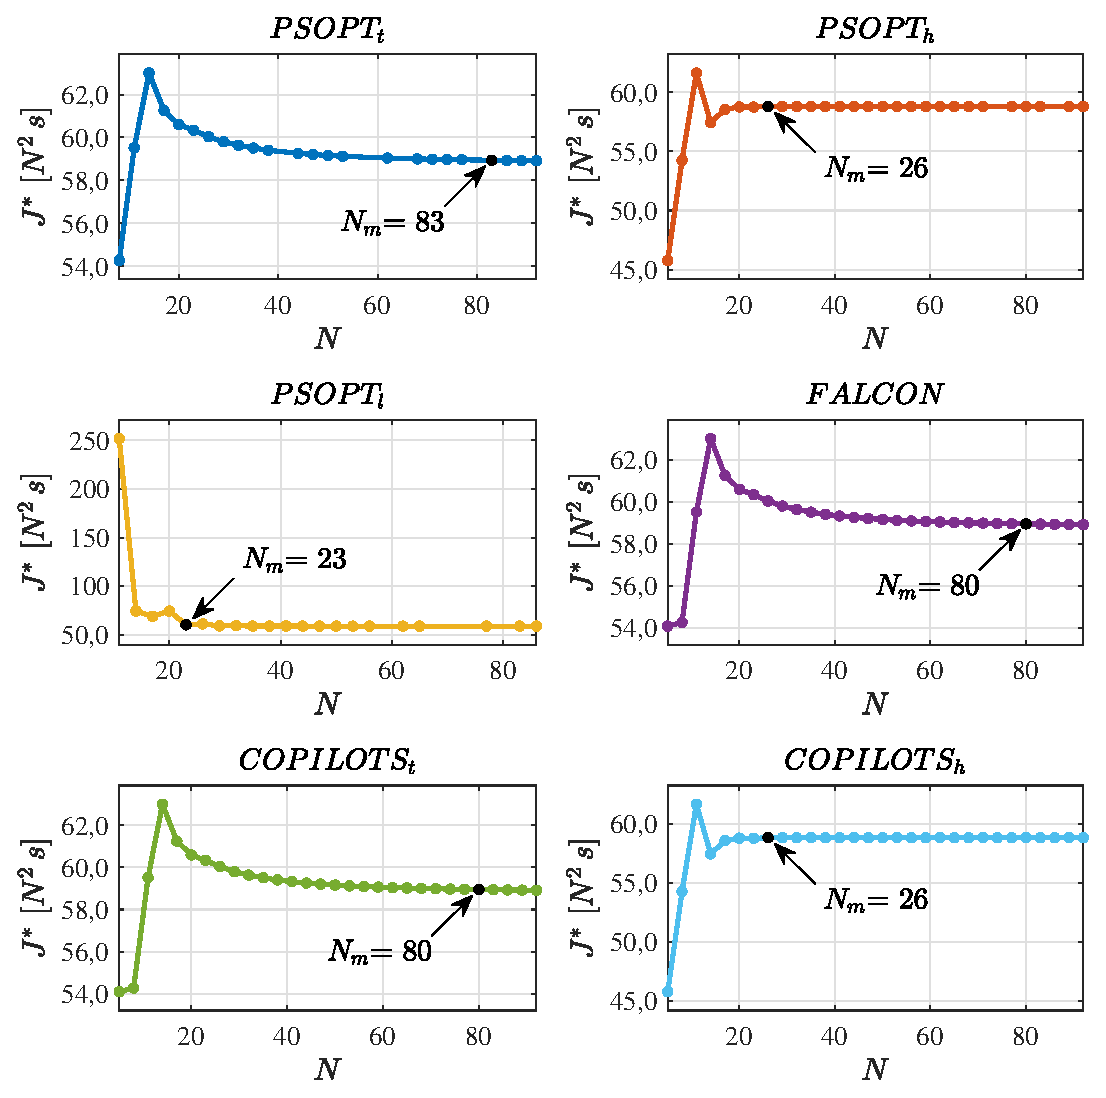
\includegraphics[scale=0.7]{fig/resultados/penduloInvertido/sens/J}
	\captionof{figure}[Influência do número de nós de colocação no valor da função objetivo para o problema do pêndulo invertido]{
	Influência do número de nós de colocação $ N $ no valor da função objetivo $ J^* $ para o problema do pêndulo invertido.}
	\label{fig:penduloInvertido:sensibilidade:J}
	\vspace{\onelineskip}
\end{minipage}

\todo[inline, color=pink, size=normalsize]{Análise dos gráficos $ J \times N $}

Nesta figura observa-se que, após um determinado valor para $N_m$, todos os pacotes convergiram para a solução reportada na literatura (\textcolor{red}{Inserir por favor o valor da função objetivo e a referência}). Todavia, deve ser mencionado que não foi possível, empregando o $ PSOPT_t $, o $ PSOPT_h $ e o $ PSOPT_l $, obter soluções para todos os $ N $ considerados. Em contrapartida, o valor de $ J^* $ para o $ PSOPT_l $ convergiu mais rapidamente que aqueles requeridos pelas outras abordagens. Os valores entre $ J^* $ e $ N $ associadas a cada um dos métodos que fazem uso de colocação trapezoidal ($ FALCON $, o $ PSOPT_t $ e $ COPILOTS_t $) foram semelhantes entre si. Esta concordância pode ser verificada quando comparam-se os resultados obtidos peplo $ PSOPT_h $ e $ COPILOTS_h $, ambos métodos que empregam a colocação Hermite-Simpson. Além disso, observa-se que os valores de  $ J^* $ referentes aos métodos que empregam a colocação trapezoidal aumentam até atingir seu valor máximo e depois voltam a cair até alcançar a convergência, estando o pico de $ J^* $ associado a $ N = 14 $. Nesse caso, escolheu-se $ N_m $ utilizando a métrica proposta originalmente, porém, desconsiderando-se os $ J^* $ obtidos para $ N < 14 $. De forma análoga, observa-se que os $ J^* $ associados aos métodos que fazem uso da colocação Hermite-Simpson crescem até $ N = 11 $, depois sofrem uma queda brusca em $ N = 14 $, para em seguida voltarem a crescer lentamente até atingir a convergência. Para estes casos considera-se que esse no aumento no valor da função objetivo se deve ao pequeno número de nós de colocação associado à violações nas restrições, o que implica em valores de $J$ não coerentes com o reportado \cite{kelly_introduction_2017}. Assim como observado para o problema anterior, ressalta-se a importância da realização de análise de sensibilidade no que tange o número de nós de colocação, bem como da análise do atendimento das restrições do estudo em questão.

\todo[inline, color=pink, size=normalsize]{Introdução dos resultados $ N = N_m $}

As métricas calculadas por cada um dos pacotes são apresentadas Tabela \ref{tab:penduloInvertido:raw} considerando $N=N_m$. Nesta tabela tem-se o valor da função objetivo ($ J^* $), o tempo de processamento médio ($ t_p $), o desvio padrão atribuído ($ s_t $), a máxima violação das restrições ($ \Delta c_{max} $) e o número de execuções bem sucedidas ($ N_s $).

\begin{table}[!h]
	\centering
	\caption[Métricas  obtidas  para  o  problema  do pêndulo invertido]{Métricas  obtidas  para  o  problema  do pêndulo invertido. Os melhores $ N_m $, $ J^* $, $ t_p $, $ n_{aval} $ e $ N_s\% $ se encontram destacados.}
	\label{tab:penduloInvertido:raw}
	\begin{tabular}{@{}ccccccccc@{}}
		\toprule
		Método       & $N_m$                              & $J^*$                                    & $t_p$ {[}$s${]}                         & $s_t$ {[}$s${]} & $n_{aval}$                         & $\Delta c_{max}$                         & $N_s$ & $N_s\%$                                  \\ \midrule
		$PSOPT_t$    & 83                                 & 58,93880                                 & 1,86743                                 & 0,18145         & 542                                & 4,32e-14                                 & 24    & 80,00\%                                  \\
		$PSOPT_h$    & 26                                 & {\color[HTML]{009901} \textbf{58,80540}} & 0,59690                                 & 0,04756         & 221                                & 2,78e-14                                 & 28    & 93,33\%                                  \\
		$PSOPT_l$    & {\color[HTML]{009901} \textbf{23}} & 60,16670                                 & 0,43817                                 & 0,01904         & 47                                 & 6,64e-14                                 & 21    & 70,00\%                                  \\
		$FALCON$     & 80                                 & 58,94871                                 & {\color[HTML]{009901} \textbf{0,18535}} & 0,03597         & {\color[HTML]{009901} \textbf{34}} & 9,32e-11                                 & 30    & {\color[HTML]{009901} \textbf{100,00\%}} \\
		$COPILOTS_t$ & 80                                 & 58,94871                                 & 16,46423                                & 0,08403         & 27044                              & 1,55e-15 & 30    & {\color[HTML]{009901} \textbf{100,00\%}} \\
		$COPILOTS_h$ & 26                                 & 58,80543                                 & 17,42163                                & 0,63533         & 34017                              & 2,28e-15                                 & 30    & {\color[HTML]{009901} \textbf{100,00\%}} \\ \bottomrule
	\end{tabular}
\end{table}

\todo[inline, color=pink, size=normalsize]{Análise dos resultados $ N = N_m $}

Nesta tabela é possível observar que os valores de $ N_m $ relacionados aos métodos que fazem uso da colocação trapezoidal ($ FALCON $, $ PSOPT_t $ e $ COPILOTS_t $)  se mostraram bem próximos uns dos outros e bem maiores que os computados pelos demais métodos. O $ PSOPT_l $ foi o que resultou no menor valor para $ N_m $. Já o maior valor de função objetivo foi encontrado pelo $ PSOPT_l $. Apesar do elevado valor de $ N_m $ requerido pelo $ FALCON $, verifica-se que a esse não está diretamente associado os menores valores de $ t_p $ e de $ n_{aval} $. Os valores de $ t_p $ e de $ n_{aval} $ associados ao $ COPILOTS $, independentemente do tipo de colocação considerado, são bem maiores que os requeridos pelos demais pacotes. Em contrapartida, verifica-se que o $ COPILOTS_h $ e o $ PSOPT_h $ convergiram para valores próximos ao melhor encontrado. O parâmetro $ N_m $ requerido pelo $ COPILTS_h $ é cerca de três vezes menor que o associado ao $ COPILOTS_t $. Ainda assim, o $ COPILOTS_h $ requeriu um valor de $ n_{aval} $ menor com relação ao $ COPILOTS_t $. Finalmente, ressalta-se que somente o $ FALCON $ e o $ COPILOTS $ foram capazes de encontrar a solução para todos os valores de $ N $ considerados. 

\todo[inline, color=pink, size=normalsize]{Introdução das trajetórias}

Os perfis referentes as variáveis de estado e controle considerando $ N = N_m $ são apresentadas nas Figuras \ref{fig:penduloInvertido:x:d}-\ref{fig:penduloInvertido:u:F}. 
Nestas figuras é possível observar boa concordância entre todos os perfis. A única trajetória de controle um pouco discrepante foi obtida pelo $ PSOPT_l $, em que são observadas pequenas oscilações no início e no fim da trajetória. Esse comportamento pode estar relacionado como é realizada a interpolação da trajetória de controle neste pacote.

\noindent
\begin{minipage}{\textwidth}
	\vspace{\onelineskip}
	\centering
	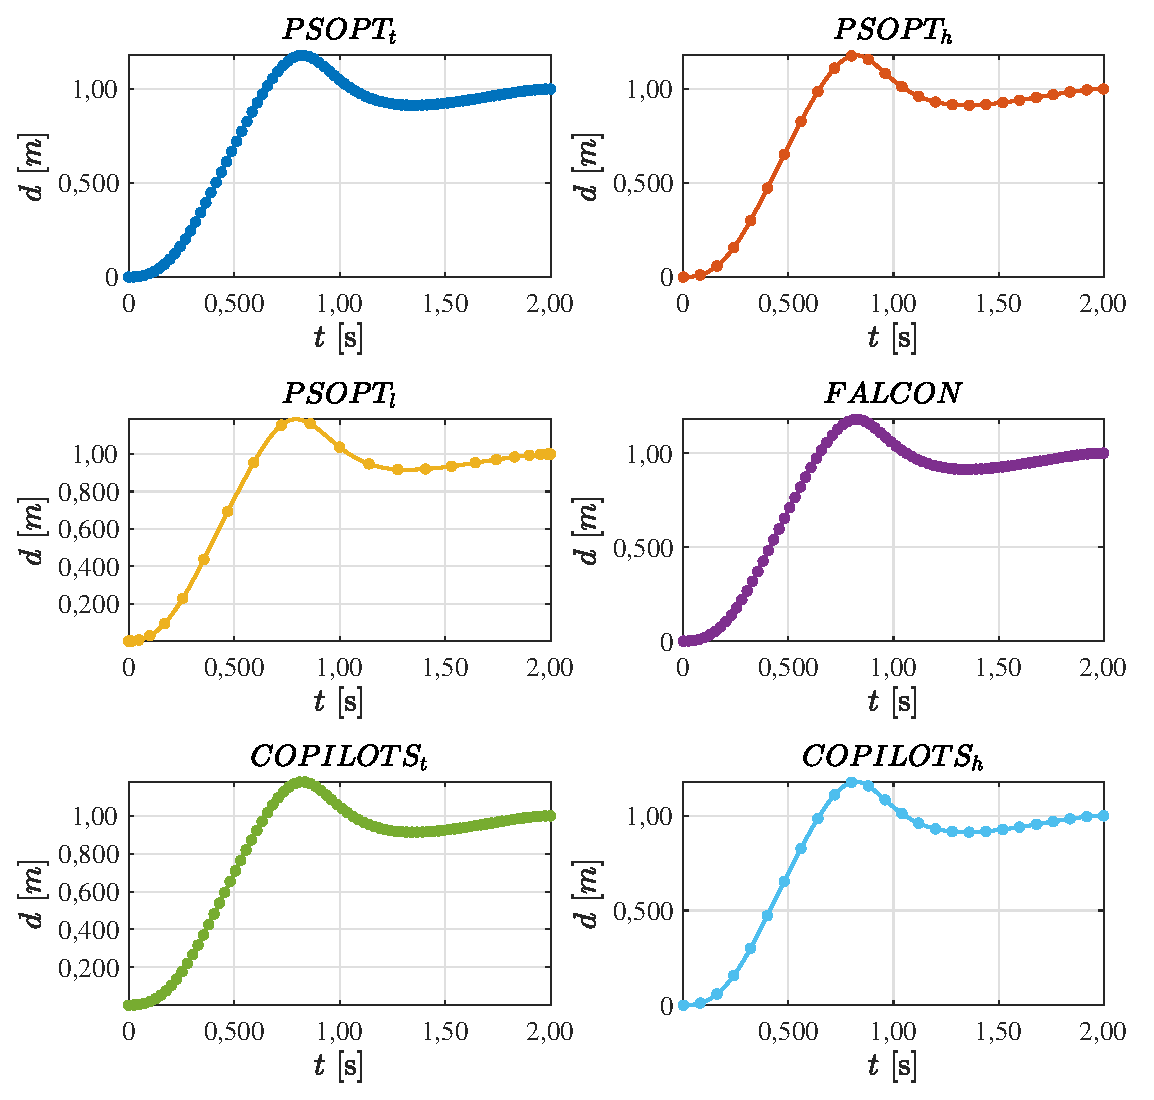
\includegraphics[scale=0.7]{fig/resultados/penduloInvertido/traj/x/d}
	\captionof{figure}[Variável de estado $d(t)$ para o problema do pêndulo]{Variável de estado $d(t)$ para o problema do pêndulo. Os pontos representam os valores discretizados e as linhas contínuas representam as trajetórias interpoladas.}
	\label{fig:penduloInvertido:x:d}
	\vspace{\onelineskip}
\end{minipage}

\noindent
\begin{minipage}{\textwidth}
	\vspace{\onelineskip}
	\centering
	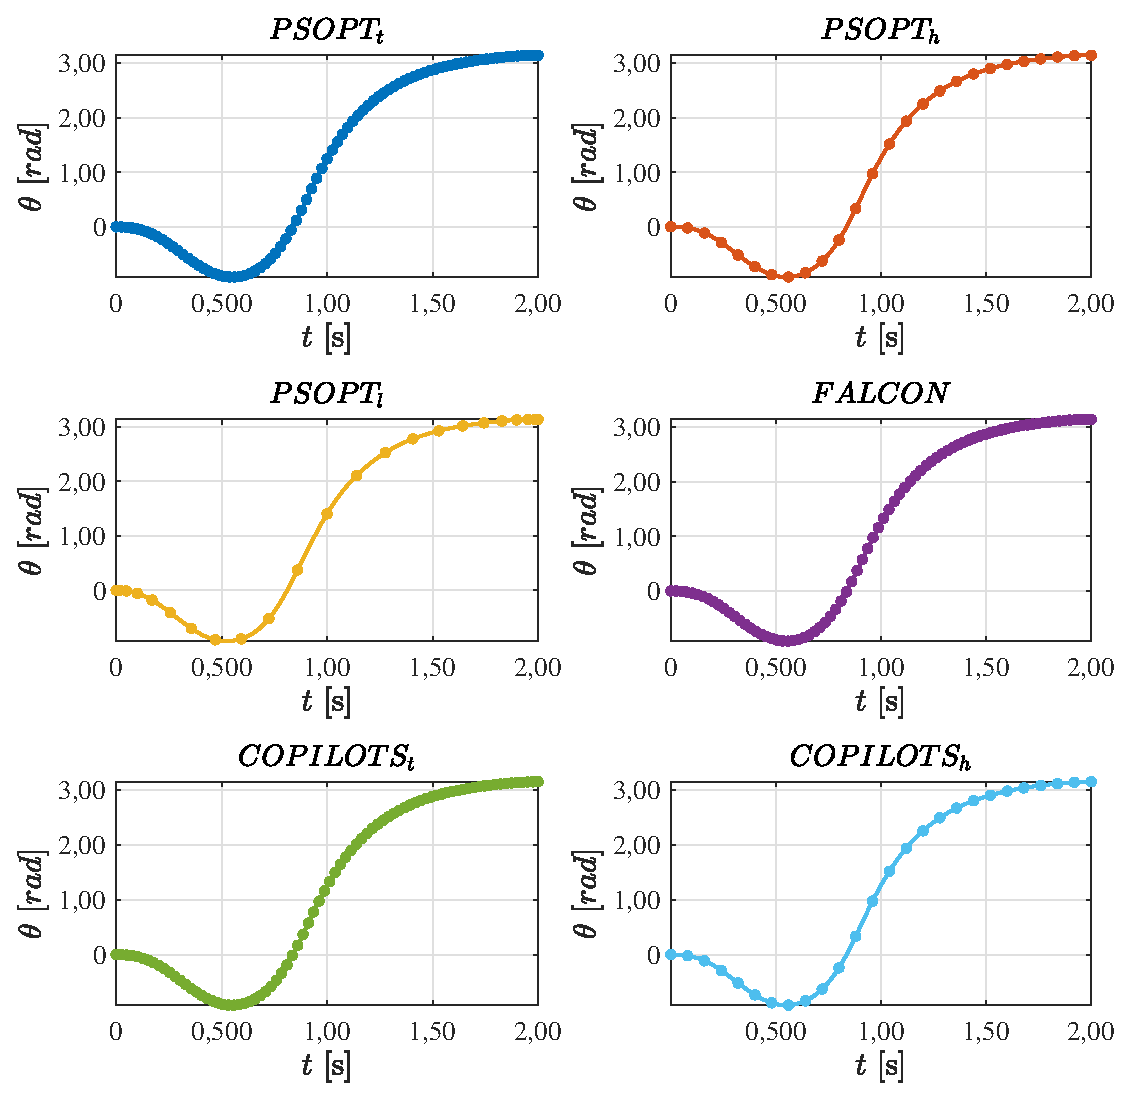
\includegraphics[scale=0.7]{fig/resultados/penduloInvertido/traj/x/theta}
	\captionof{figure}[Variável de estado $\theta(t)$ para o problema do pêndulo]{Variável de estado $\theta(t)$ para o problema do pêndulo. Os pontos representam os valores discretizados e as linhas contínuas representam as trajetórias interpoladas.}
	\label{fig:penduloInvertido:x:theta}
	\vspace{\onelineskip}
\end{minipage}

\noindent
\begin{minipage}{\textwidth}
	\vspace{\onelineskip}
	\centering
	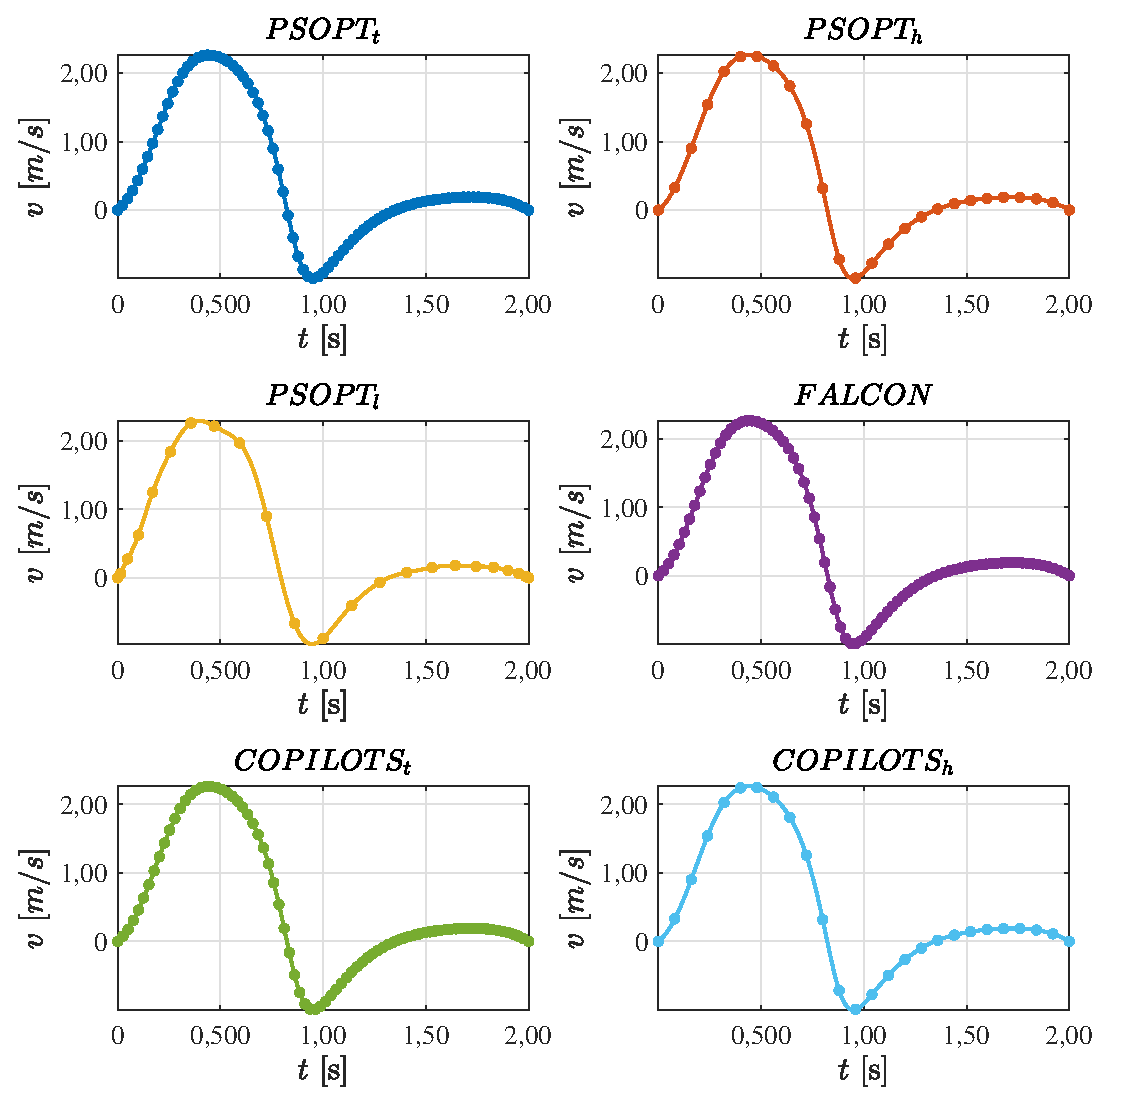
\includegraphics[scale=0.7]{fig/resultados/penduloInvertido/traj/x/v}
	\captionof{figure}[Variável de estado $v(t)$ para o problema do pêndulo]{Variável de estado $v(t)$ para o problema do pêndulo. Os pontos representam os valores discretizados e as linhas contínuas representam as trajetórias interpoladas.}
	\label{fig:penduloInvertido:x:v}
	\vspace{\onelineskip}
\end{minipage}

\noindent
\begin{minipage}{\textwidth}
	\vspace{\onelineskip}
	\centering
	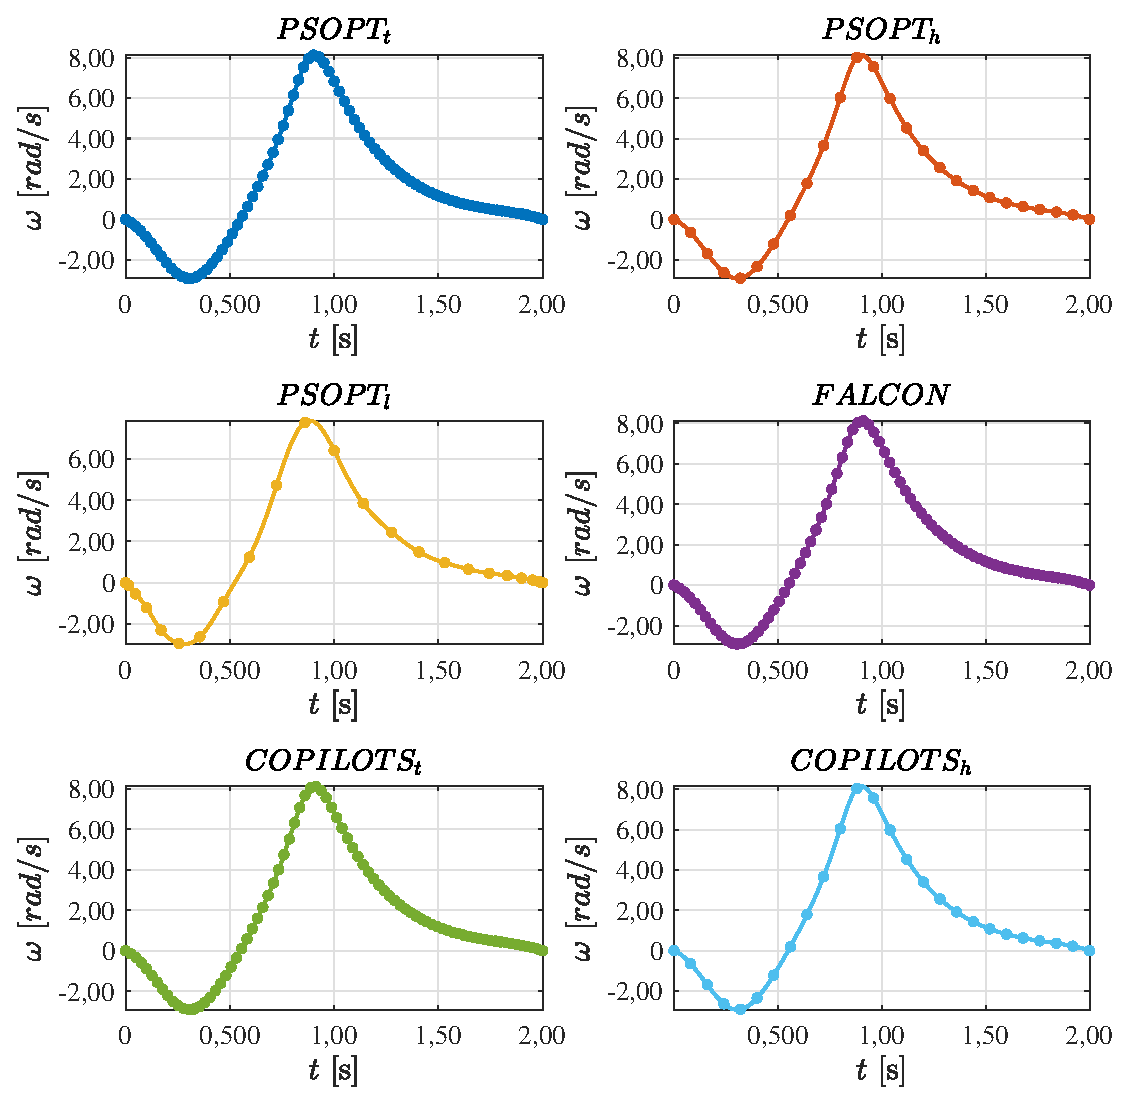
\includegraphics[scale=0.7]{fig/resultados/penduloInvertido/traj/x/omega}
	\captionof{figure}[Variável de estado $\omega(t)$ para o problema do pêndulo]{Variável de estado $\omega(t)$ para o problema do pêndulo. Os pontos representam os valores discretizados e as linhas contínuas representam as trajetórias interpoladas.}
	\label{fig:penduloInvertido:x:omega}
	\vspace{\onelineskip}
\end{minipage}

\noindent
\begin{minipage}{\textwidth}
	\vspace{\onelineskip}
	\centering
	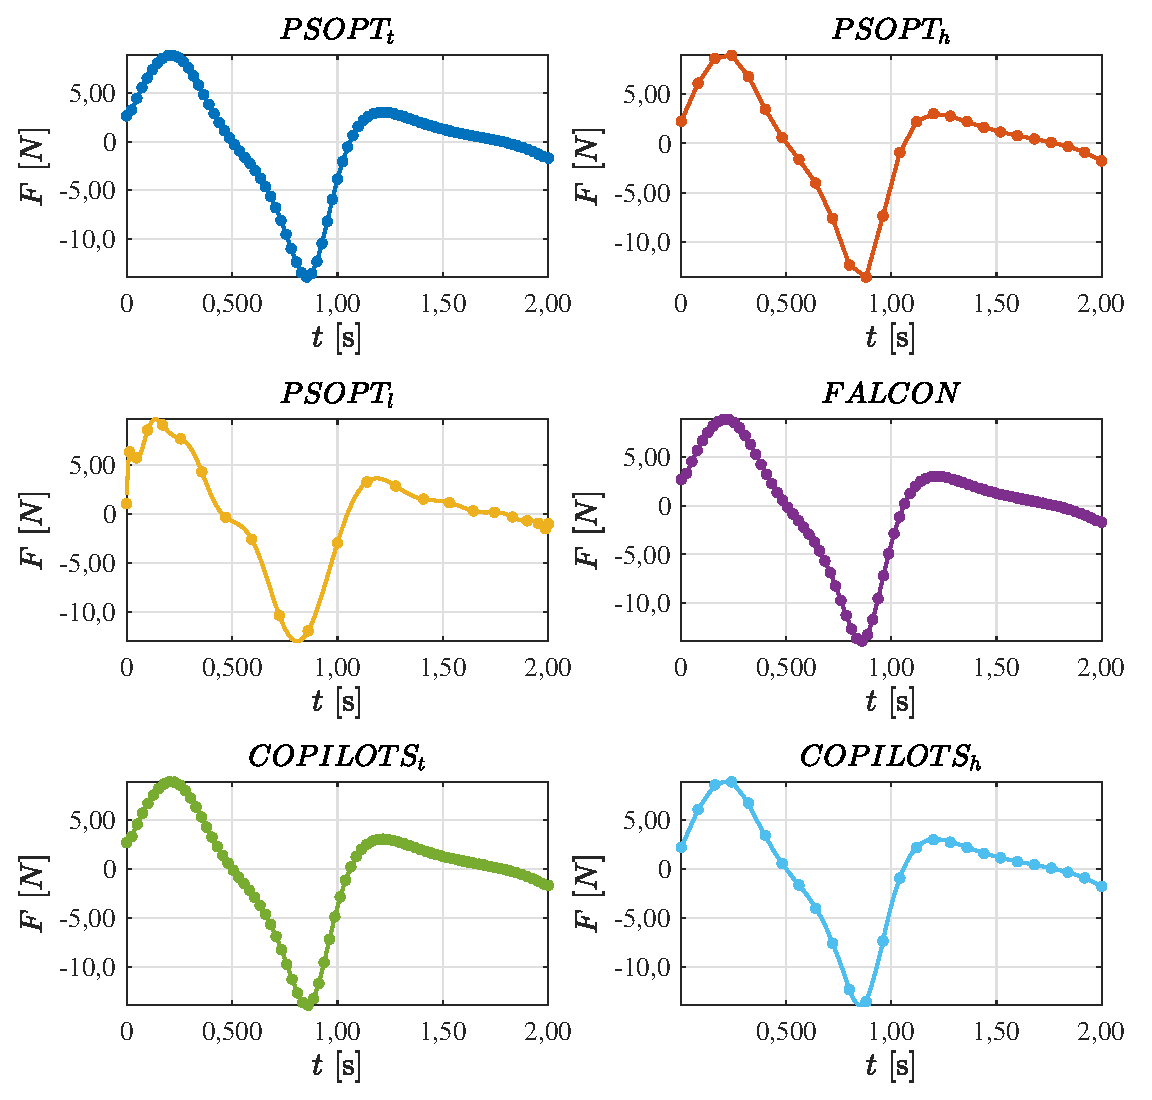
\includegraphics[scale=0.7]{fig/resultados/penduloInvertido/traj/u/F}
	\captionof{figure}[Variável de controle $F(t)$ para o problema do pêndulo]{Variável de controle $F(t)$ para o problema do pêndulo. Os pontos representam os valores discretizados e as linhas contínuas representam as trajetórias interpoladas.}
	\label{fig:penduloInvertido:u:F}
	\vspace{\onelineskip}
\end{minipage}

\todo[inline, color=pink, size=normalsize]{Análise das trajetórias}

\todo[inline, color=pink, size=normalsize]{Apresentação dos gráficos de trajetória complexos caso haja}

Já a Figura \ref{fig:penduloInvertido:avancado} apresenta a  vista lateral do pêndulo invertido, na qual são representadas algumas das posições durante a execução da manobra de \textit{swing-up}. A construção desse gráfico foi baseada nos resultados obtidos pelo $ COPILOTS_h $, o qual está associado ao menor valor de $ J^* $. Vale ressaltar que a posição da extremidade do pêndulo $ \big( x_e(t), y_e(t) \big) $ pode ser determinada com base nas relações $ x_e(t) = d(t) + l \, \sin\big( \theta(t) \big) $ e $ y_e(t) = l \, \cos \big( \theta(t) \big) $. Assim sendo, os pontos nesta figura representam os $ \big( x_e(t), y_e(t) \big) $ obtidos a partir dos valores calculados por $ d(t) $ e $ \theta(t) $ nos nós de colocação, enquanto a linha continua que conecta esses pontos representa a trajetória computada com base nas trajetórias apresentadas nas Figuras \ref{fig:penduloInvertido:x:d} e \ref{fig:penduloInvertido:x:theta}.

\noindent
\begin{minipage}{\textwidth}
	\vspace{\onelineskip}
	\centering
	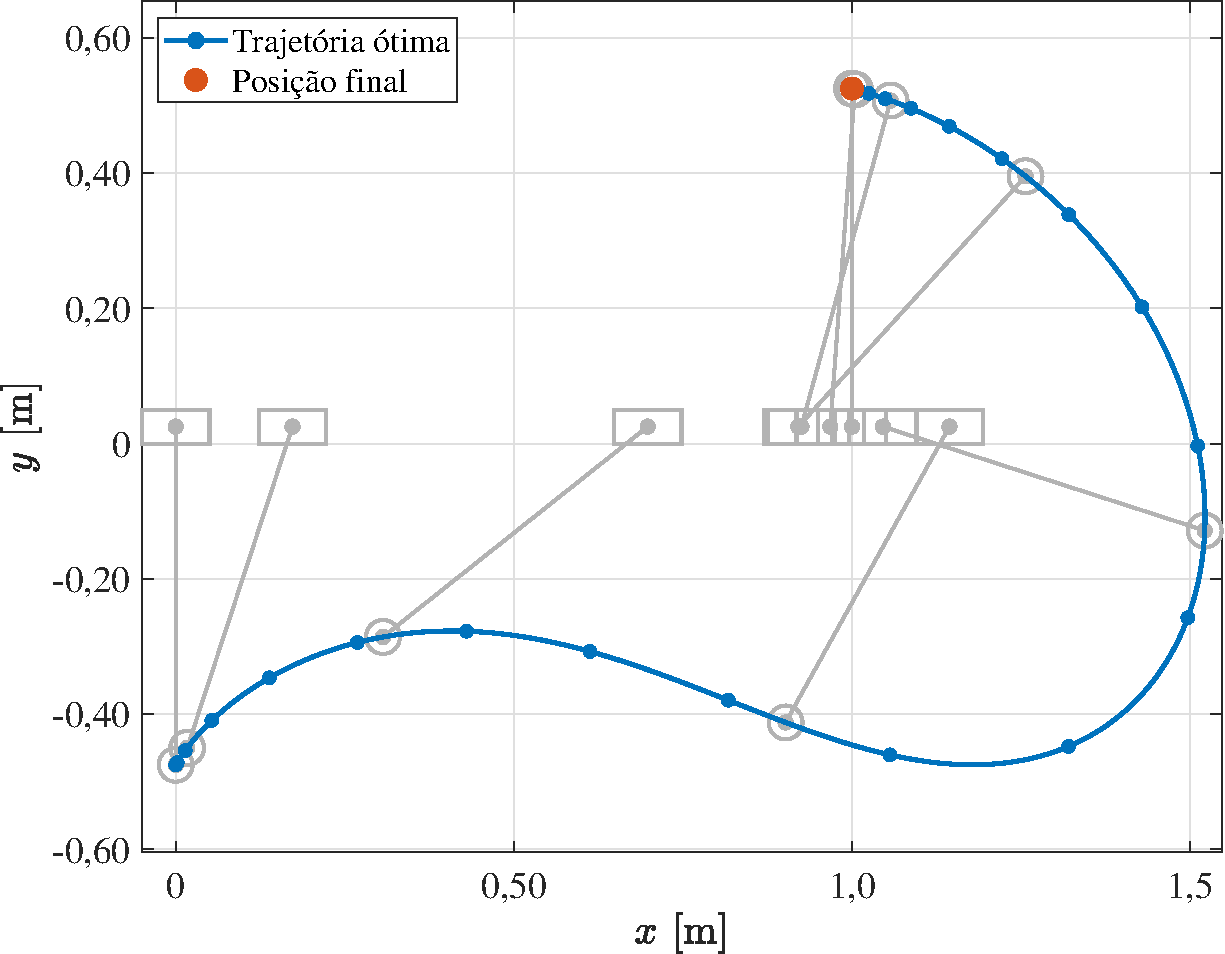
\includegraphics[scale=0.5]{fig/resultados/penduloInvertido/obs/adv}
	\captionof{figure}[Algumas posições do pêndulo invertido durante a execução da manobra de \textit{swing-up}]{Algumas posições do pêndulo invertido durante a execução da manobra de \textit{swing-up}.}
	\label{fig:penduloInvertido:avancado}
	\vspace{\onelineskip}
\end{minipage}

\todo[inline, color=pink, size=normalsize]{Introdução dos resultados $ t_p \times N $ e $ n_{aval} \times N $}

Para avalar a influência do número de nós de colocação no tempo de processamento e no número de avaliações da função objetivo são apresentadas nas Figuras \ref{fig:penduloInvertido:sensibilidade:t} e \ref{fig:penduloInvertido:sensibilidade:naval}. Nestes gráficos são apresentadas as variações: $ \Delta t_p = \max\{t_p\} - \min\{t_p\} $ e $ \Delta n_{aval} = \max\{n_{aval}\} - \min\{n_{aval}\} $. Os pontos nos gráficos representam os valores atribuídos a $ t_p $ (e a $ n_{aval} $) para cada um dos $ N $ considerados, enquanto as linhas contínuas representam curvas de tendência, obtidas por meio de regressões lineares, em que $R^2$ é o coeficiente de determinação. Os valores de $ N $ empregados na geração desses resultados são iguais àqueles considerados na computação da relação entre $ J^* $ e $ N $.

Nestas figuras é possível verificar que, de forma geral, ambos os valores de $ t_p $ e de $ n_{aval} $ aumentam com o incremento no valor do número de nós de colocação, conforme esperado. Além disso, em todas as configurações analisadas, os resultados obtidos pelo $ FALCON $ se mostram pouco sensíveis ao aumento de $ N $ em relação ao tempo e ao número de avaliações da função objetivo, conforme observado para $ \Delta t_p $ e $ \Delta n_{aval} $. Tal comportamento pode ser justificado pelo uso de informações simbólicas, o que na prática, facilita o cômputo de gradientes, necessários para a resolução do PPNL correspondente. Por outro lado, os valores de $ t_p $ e de $ n_{aval} $ associados ao $ COPILOTS $ se mostraram consideravelmente mais sensíveis ao aumento de $ N $ com relação as outras abordagens, conforme constatado avaliando-se $ \Delta t_p $ e $ \Delta n_{aval} $. Para este caso, imagina-se que estes valores elevados com relação à outras abordagens esteja relacionado a metodologia empregada para a resolução do PPNL associado. 

Já o tempo de processamento associado ao $ PSOPT_l $ se mostrou mais sensível ao aumento de $ N $ em relação ao $ PSOPT_t $ e ao $ PSOPT_h $. No entanto, os valores de $ n_{aval} $ associados ao $ PSOPT_t $, ao $ PSOPT_h $ e ao $ PSOPT_l $ se mostraram igualmente sensíveis ao aumento de $ N $, conforme pode ser observado ao se comparar os valores de $ \Delta n_{aval} $ para cada um. Para alguns dos $ N $ considerados, é possível verificar picos nos $ n_{aval} $ associados ao $ PSOPT_t $ e ao $ PSOPT_h $, o que justifica os baixos $ R^2 $ atribuídos a esses métodos. A presença desses picos pode ser justificada pela forma como cada pacote realiza a sua inicialização. Além disso, picos bastante similares podem ser observados nos valores de $ t_p $ e de $ n_{aval} $ associados ao $ COPILOTS_t $.

\noindent
\begin{minipage}{\textwidth}
	\vspace{\onelineskip}
	\centering
	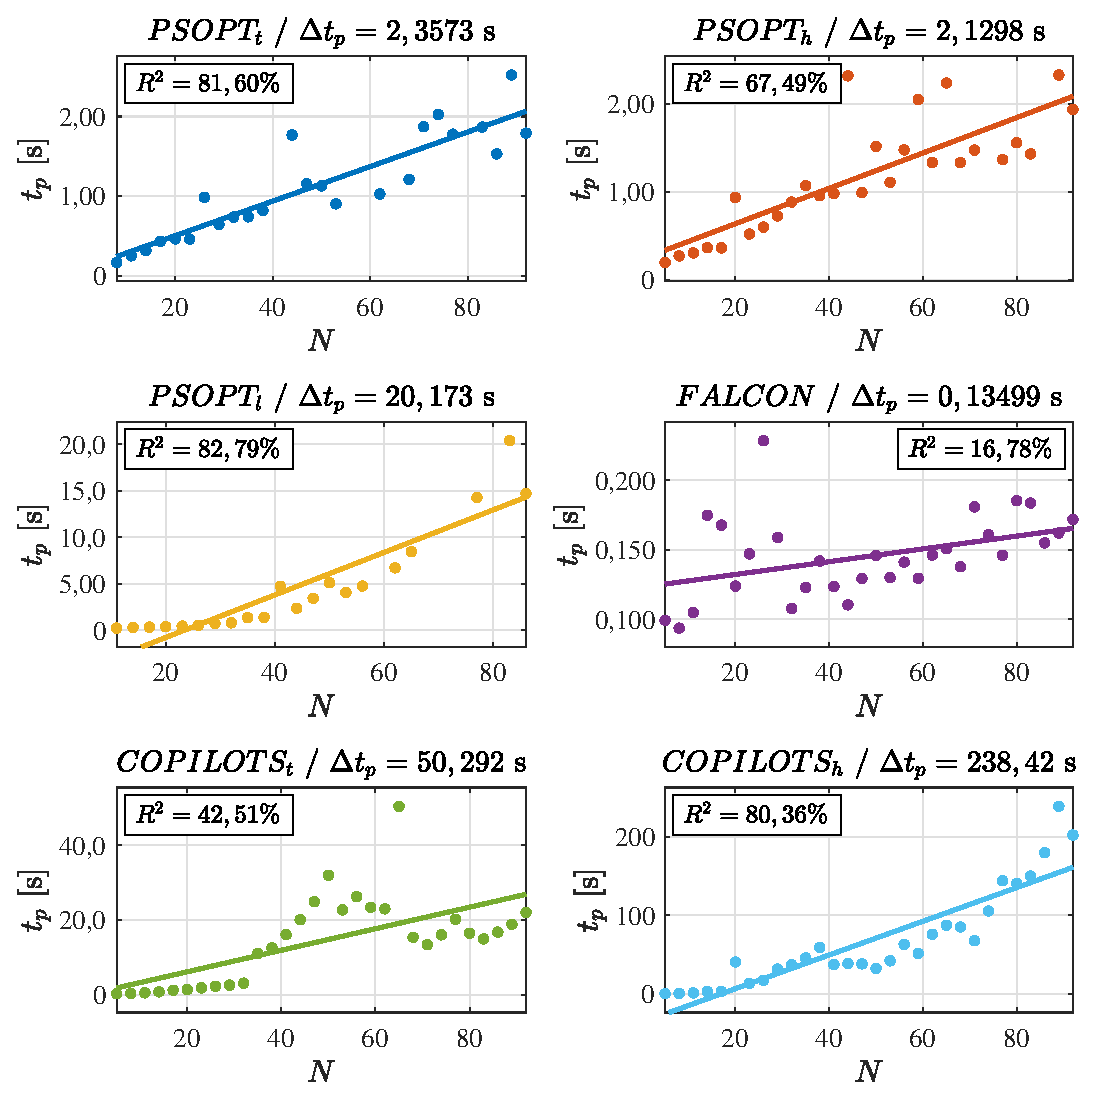
\includegraphics[scale=0.7]{fig/resultados/penduloInvertido/sens/t}
	\captionof{figure}[Relação entre o tempo de processamento e o número de nós de colocação para o problema do pêndulo invertido]{Relação entre o tempo de processamento $ t_p $ e o número de nós de colocação $ N $ para o problema do pêndulo invertido.}
	\label{fig:penduloInvertido:sensibilidade:t}
	\vspace{\onelineskip}
\end{minipage}

A Figura \ref{fig:penduloInvertido:sensibilidade:J} apresenta um comportamento diferente do esperado, isto é; espera-se que $ J^* $ diminua com o crescimento de $ N $, no entanto, para $ N < 14 $, verifica-se que ocorre o oposto. Anteriormente foi apresentada uma justificativa que leva em consideração o número de nós de colocação bem como o atendimento das restrições. Para explicar tal comportamento do ponto de vista matemático, serão avaliadas estratégias para a integração da função objetivo $ J $.   

Como a solução analítica do estudo de caso não é conhecida  \cite{kelly_introduction_2017}, será considerado como solução de referência aquela obtida usando o $ FALCON $ para $ N = 2000 $. Este foi escolhido por apresentar um comportamento suave para a variável de controle. De posse deste perfil, pode determinar o valor do referido objetivo.

\noindent
\begin{minipage}{\textwidth}
	\vspace{\onelineskip}
	\centering
	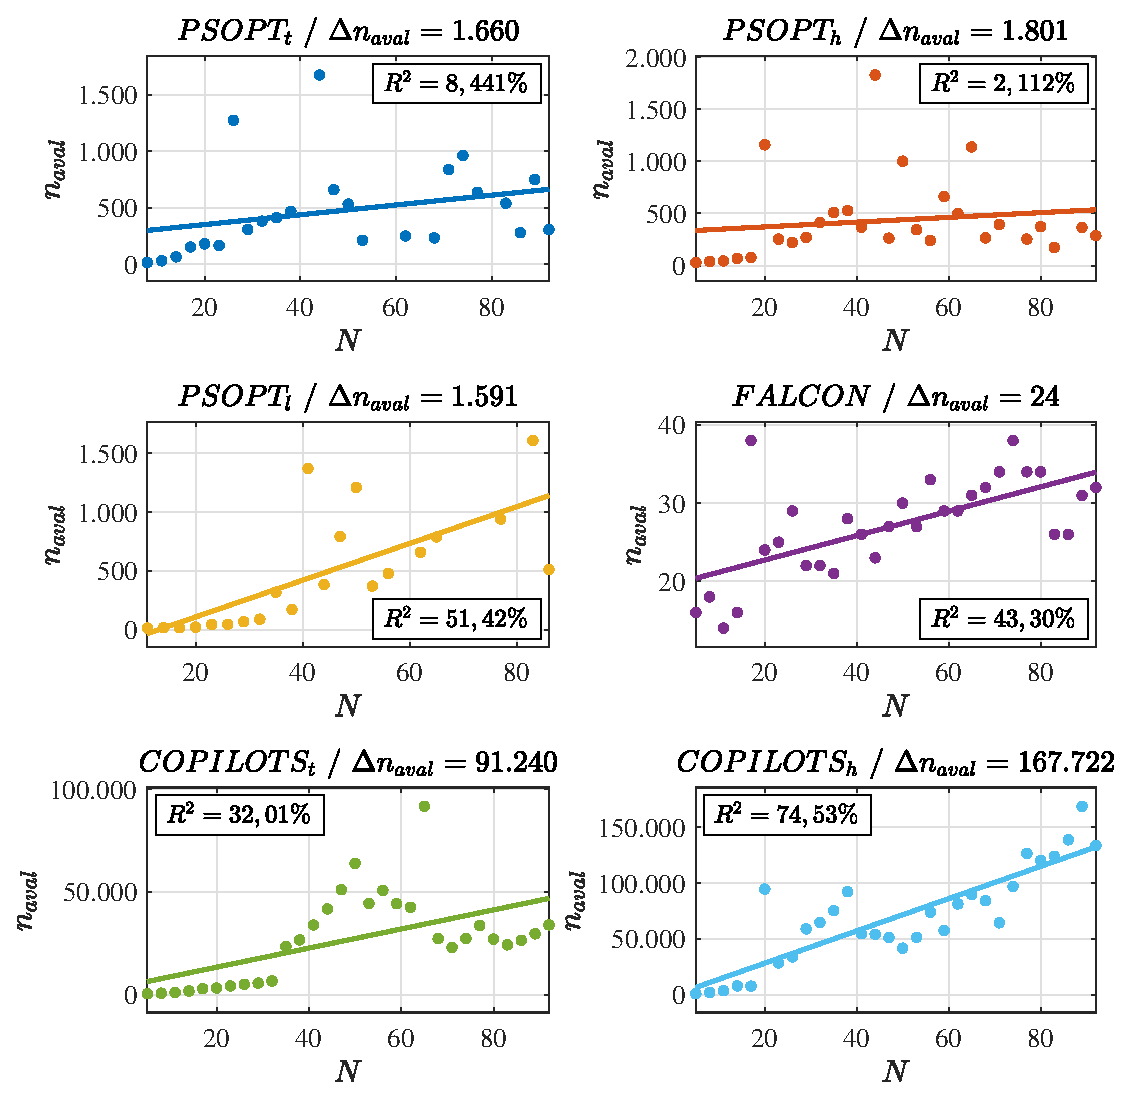
\includegraphics[scale=0.7]{fig/resultados/penduloInvertido/sens/eval}
	\captionof{figure}[Relação entre o número de avaliações da função objetivo e o número de nós de colocação para o problema do pêndulo invertido]{Relação entre o número de avaliações da função objetivo $ n_{aval} $ e o número de nós de colocação $ N $ para o problema do pêndulo invertido.}
	\label{fig:penduloInvertido:sensibilidade:naval}
	\vspace{\onelineskip}
\end{minipage}

\todo[inline, color=pink, size=normalsize]{Análise dos resultados $ t_p \times N $ e $ n_{aval} \times N $}

Ao se aplicar colocação trapezoidal, o cálculo da integral associada ao custo é realizada via uso de quadratura trapezoidal. As Figuras \ref{fig:penduloInvertido:trap:N=7}, \ref{fig:penduloInvertido:trap:N=9} e \ref{fig:penduloInvertido:trap:N=11} apresentam as aproximações lineares nas quais se baseia a computação de $ \int_{0}^{t_f} F^2(t) dt $ considerando $ N = 7 $, $ N = 9 $ e $ N = 11 $, respectivamente. Nota-se que o maior pico de $ F^2(t) $, que ocorre em $ t = 0,85 $ s, não é capturado para pequenos valores de $ N $. Desta forma, o valor atribuído a $ \int_{0}^{t_f} F^2(t) dt $ via quadratura trapezoidal acaba sendo bem menor que o valor verdadeiro, o que justifica os baixos $ J^* $ observados para $ N < 14 $, conforme ilustrado na Figura \ref{fig:penduloInvertido:sensibilidade:J}. 

Já na Figura \ref{fig:penduloInvertido:trap:NvsJ} é apresentada a relação entre o valor atribuído a $ \int_{0}^{t_f} F^2(t) dt $ via  quadratura trapezoidal e o número de nós de colocação $ N $. Como esperado, nota-se que o valor de $ J $ tende a estabilizar e convergir para a solução ótimo à medida que $ N $ cresce. Além disso, observa-se que tal convergência ocorre para $ N > 12 $, o que justifica os resultados obtidos conforme a Figura \ref{fig:penduloInvertido:sensibilidade:J}. 

\noindent	
\begin{minipage}{\textwidth}
	\vspace{\onelineskip}
	\centering
	\includegraphics[scale=0.7]{fig/resultados/penduloInvertido/obs/trap/N=7}
	\captionof{figure}[Aproximações lineares para a avaliação de integrais usando quadratura trapezoidal ($ N = 7 $) no $ FALCON $]{Aproximações lineares para a avaliação de integrais usando quadratura trapezoidal ($ N = 7 $) no $ FALCON $.}
	\label{fig:penduloInvertido:trap:N=7}
	\vspace{\onelineskip}
\end{minipage}

\noindent	
\begin{minipage}{\textwidth}
	\vspace{\onelineskip}
	\centering
	\includegraphics[scale=0.7]{fig/resultados/penduloInvertido/obs/trap/N=9}
	\captionof{figure}[Aproximações lineares para a avaliação de integrais usando quadratura trapezoidal ($ N = 9 $) no $ FALCON $]{Aproximações lineares para a avaliação de integrais usando quadratura trapezoidal ($ N = 9 $) no $ FALCON $.}
	\label{fig:penduloInvertido:trap:N=9}
	\vspace{\onelineskip}
\end{minipage}

Analogamente, é possível analisar os resultados obtidos considerando a colocação Hermite-Simpson. Para essa finalidade, nas Figuras \ref{fig:penduloInvertido:hersim:N=7}, \ref{fig:penduloInvertido:hersim:N=9} e \ref{fig:penduloInvertido:hersim:N=11} são representadas as aproximações quadráticas nas quais se baseia o cálculo de $ \int_{0}^{t_f} F^2(t) dt $ via quadratura de Simpson considerando $ N = 7 $, $ N = 9 $ e $ N = 11 $, respectivamente. Nesta figura, observa-se que o maior pico de $ F^2(t) $ não é satisfatoriamente representado na estimativa da integral em questão para $ N $ pequenos, o que pode justificar os menores valores de $J$ em relação à solução reportada na literatura. 

Na Figura \ref{fig:penduloInvertido:hersim:NvsJ} é apresentada a relação entre o valor da $ \int_{0}^{t_f} F^2(t) dt $ via quadratura de Simpson em função do parâmetro $ N $. Como esperado, o aumento no valor deste parâmetro implica na melhor aproximação da integral, o que na prática implica em uma melhor precisão. Neste caso, observa-se que tal convergência ocorre para $ N > 16 $, o que justifica os resultados verificados quando avalia-se a relação entre $ N $ e $ J^* $ apresentado na Figura \ref{fig:penduloInvertido:sensibilidade:J}.

Em resumo, a qualidade da solução encontrada em qualquer procedimento numérico sempre é função dos parâmetros que caracterizam a metodologia, bem como do nível de sofisticação da abordagem numérica empregada. No 
PCO isso não é diferente, isto é; a qualidade da solução também é função do nível de discretização informado pelo usuário (ou computado pela rotina considerada). Neste caso, sempre é importante realizar a análise de sensibilidade no que tange o efeito do número de nós ou pontos de colocação empregados.

\noindent	
\begin{minipage}{\textwidth}
	\vspace{\onelineskip}
	\centering
	\includegraphics[scale=0.7]{fig/resultados/penduloInvertido/obs/trap/N=11}
	\captionof{figure}[Aproximações lineares para a avaliação de integrais usando quadratura trapezoidal ($ N = 11 $) no $ FALCON $]{Aproximações lineares para a avaliação de integrais usando quadratura trapezoidal ($ N = 11 $) no $ FALCON $.}
	\label{fig:penduloInvertido:trap:N=11}
	\vspace{\onelineskip}
\end{minipage}

\noindent	
\begin{minipage}{\textwidth}
	\vspace{\onelineskip}
	\centering
	\includegraphics[scale=0.7]{fig/resultados/penduloInvertido/obs/trap/NvsJ}
	\captionof{figure}[Relação entre o valor atribuído a função objetivo via quadratura trapezoidal em função do número de nós de colocação]{Relação entre o valor atribuído a função objetivo via quadratura trapezoidal em função do número de nós de colocação.}
	\label{fig:penduloInvertido:trap:NvsJ}
	\vspace{\onelineskip}
\end{minipage}

\noindent	
\begin{minipage}{\textwidth}
	\vspace{\onelineskip}
	\centering
	\includegraphics[scale=0.7]{fig/resultados/penduloInvertido/obs/hersim/N=7}
	\captionof{figure}[Função objetivo via quadratura de Simpson para o problema do pêndulo invertido ($N$=7)]{Função objetivo via quadratura de Simpson para o problema do pêndulo invertido ($N$=7).}
	\label{fig:penduloInvertido:hersim:N=7}
	\vspace{\onelineskip}
\end{minipage}

\noindent	
\begin{minipage}{\textwidth}
	\vspace{\onelineskip}
	\centering
	\includegraphics[scale=0.7]{fig/resultados/penduloInvertido/obs/hersim/N=9}
	\captionof{figure}[Função objetivo via quadratura de Simpson para o problema do pêndulo invertido ($N$=9)]{Função objetivo via quadratura de Simpson para o problema do pêndulo invertido ($N$=9).}
	\label{fig:penduloInvertido:hersim:N=9}
	\vspace{\onelineskip}
\end{minipage}

\noindent	
\begin{minipage}{\textwidth}
	\vspace{\onelineskip}
	\centering
	\includegraphics[scale=0.7]{fig/resultados/penduloInvertido/obs/hersim/N=11}
	\captionof{figure}[Função objetivo via quadratura de Simpson para o problema do pêndulo invertido ($N$=11)]{Função objetivo via quadratura de Simpson para o problema do pêndulo invertido ($N$=11).}
	\label{fig:penduloInvertido:hersim:N=11}
	\vspace{\onelineskip}
\end{minipage}

\noindent	
\begin{minipage}{\textwidth}
	\vspace{\onelineskip}
	\centering
	\includegraphics[scale=0.7]{fig/resultados/penduloInvertido/obs/hersim/NvsJ}
	\captionof{figure}[Relação entre o valor da função objetivo via quadratura de Simpson e o número de nós de colocação para o problema do pêndulo invertido]{Relação entre o valor da função objetivo via quadratura de Simpson e o número de nós de colocação para o problema do pêndulo invertido.}
	\label{fig:penduloInvertido:hersim:NvsJ}
	\vspace{\onelineskip}
\end{minipage}


% estacionamento
\section{Minimização do tempo durante uma manobra de estacionamento}
\label{sec:resultados:estacionamento}
\todo[inline, color=pink, size=normalsize]{Descrição geral do problema}

O problema do estacionamento paralelo consiste na determinação da trajetória a ser percorrida por um veículo durante a realização de uma manobra de baliza, a partir do qual objetiva-se o posicionamento do automóvel em uma vaga paralela à via \cite{paromtchik_autonomous_1996}. Neste procedimento, é necessário que sejam impostas limitações à velocidade e à aceleração do automóvel de forma a garantir o conforto dos passageiros e evitar o choque com outros veículos já estacionados ou com os limites delimitados na via \cite{li_time-optimal_2016}. Assim, pretende-se determinar a trajetória a ser percorrida por um veículo para que a referida manobra seja realizada no menor tempo possível \cite{li_time-optimal_2016}. As variáveis empregadas na formulação do problema, bem como as posições inicial e final do automóvel são representadas nas Figuras \ref{fig:estacionamento:estacionamento} e \ref{fig:estacionamento:estacionamentoVia}, respectivamente.

\noindent	
\begin{minipage}{\textwidth}
	\vspace{\onelineskip}
	\centering
	\includegraphics[scale=0.14]{draw/resultados/pdf/estacionamento}
	\captionof{figure}[Representação esquemática das variáveis empregadas na formulação do problema do estacionamento]{Representação esquemática das variáveis empregadas na formulação do estudo de caso em análise.}
	\label{fig:estacionamento:estacionamento}
	\vspace{\onelineskip}
\end{minipage}

\noindent	
\begin{minipage}{\textwidth}
	\vspace{\onelineskip}
	\centering
	\includegraphics[scale=0.14]{draw/resultados/pdf/estacionamentoVia}
	\captionof{figure}[Posições inicial e final do automóvel e  dimensões da via e da vaga]{Posições inicial e final do automóvel e dimensões da via e da vaga.}
	\label{fig:estacionamento:estacionamentoVia}
	\vspace{\onelineskip}
\end{minipage}

Nestas figuras tem-se que $ l $ é a distância entre os eixos do veículo, $ m $ e $ n $ são os afastamentos entre as extremidades do automóvel e os eixos traseiro e dianteiro, respectivamente, enquanto  que $ b $ é metade da largura do mesmo. A velocidade e aceleração do ponto médio $ P(d_x, d_y) $ referente ao eixo traseiro são representadas por $ v(t) $ e $ a(t) $, respectivamente. Os pontos $ A(t) $, $ B(t) $, $ C(t) $ e $ D(t) $ são as extremidades do retângulo que delimita o veículo. O ângulo entre a velocidade do ponto médio do eixo dianteiro e a reta $ \gamma $ é dado por $ \phi(t) $. A inclinação de $ \gamma $ em relação ao eixo $ x $ é dada por $ \theta(t) $. O \textit{jerk} (ou sobre-aceleração) e a velocidade angular referente à $\phi(t)$ são denotados respectivamente por $ j(t) $ e $ \omega(t) $. A vaga na qual o veículo deve estacionar possui comprimento $ SL $ e largura $ SW $, enquanto a via na qual se encontra possui largura $ CL $. O centro instantâneo de rotação é representado pelo ponto $ CIR $. 

\todo[inline, color=pink, size=normalsize]{Descrição geral do problema - Comparação com os resultados originais}

As trajetórias de controle reportadas por \citeonline{li_time-optimal_2016} são apresentadas na Figura \ref{fig:estacionamento:original}. Tais trajetórias apresentam oscilações de alta frequência sempre que verificam-se variações bruscas em $ j(t) $ ou em $ \omega(t) $. Logo, espera-se que tais oscilações apareçam nos resultados associados aos métodos aqui avaliados, o que representa um desafio para qualquer \textit{solver} de controle ótimo. 

\noindent	
\begin{minipage}{\textwidth}
	\vspace{\onelineskip}
	\centering
	\includegraphics[scale=0.42]{fig/resultados/estacionamento/obs/original}
	\captionof{figure}[Trajetórias de controle para o problema do estacionamento reportadas pela literatura]{Trajetórias de controle para o problema do estacionamento reportadas por \citeonline{li_time-optimal_2016}.}
	\label{fig:estacionamento:original}
	\vspace{\onelineskip}
\end{minipage}

\todo[inline, color=pink, size=normalsize]{Apresentação da função objetivo}

A função objetivo a ser minimizada nesta aplicação é dada como \cite{li_time-optimal_2016}:
%
\begin{equation}
	\label{eq:estacionamento:J}
	J = t_f
\end{equation}
%
sujeito ao seguinte conjunto de restrições:
%
\begin{subequations}
\begin{equation}
\label{eq:estacionamento:dinamica}
\dot{d}_x(t) = v(t) \cos(\theta(t)),\;\;d_x(0) = SL\;\text{m}
\end{equation}
\vspace{-0.6cm}
\begin{equation}
\dot{d}_y(t) = v(t)\sin(\theta(t)),\;\; d_y(0) = d_{y0} \; \text{m}
\end{equation}
\vspace{-0.5cm}
\begin{equation}
\dot{v}(t) = a(t),\;\; v(0) = 0 \; \text{m/s}
\end{equation}
\vspace{-0.55cm}
\begin{equation}
\dot{a}(t) = j(t),\;\;  a(0) = 0 \; \text{m/s$^2$}
\end{equation}
\vspace{-0.3cm}
\begin{equation}
\dot{\theta}(t) = \frac{v(t) \tan(\phi(t))}{l},\;\;  \theta(0) = 0 \; \text{rad}
\end{equation}
\vspace{-0.5cm}
\begin{equation}
\dot{\phi}(t) = \omega(t),\;\;  \phi(0) = 0 \; \text{rad} 
\end{equation}
\end{subequations}
%
em que $t$ é o tempo ($ t_f $ é o tempo final), $ \mathbf{x}(t) = \begin{bmatrix} d_x(t) & d_y(t) & v(t) & a(t) & \theta(t) & \phi(t) \end{bmatrix}^T $ é o vetor de variáveis de estados e $ \mathbf{u}(t) = \begin{bmatrix} j(t) & \omega(t) \end{bmatrix}^T $ é o vetor de variáveis de controle.

\todo[inline, color=pink, size=normalsize]{Apresentação das restrições - Restrições laterais}

Visando garantir o conforto dos passageiros e reduzir o estresse sobre os atuadores, são impostas as restrições:
%
\begin{subequations}
\begin{equation}
\label{eq:estacionamento:laterais}
|a(t)| \leq 0,75 \text{ m/s$^2$} 
\end{equation}
\vspace{-0.6cm}
\begin{equation}
|v(t)| \leq 2 \text{ m/s} 
\end{equation}
\vspace{-0.6cm}
\begin{equation}
|\phi(t)| \leq 0,58 \text{ rad} 
\end{equation}
\vspace{-0.6cm}
\begin{equation}
|\kappa'(t)| \leq 0,6 \text{ 1/(m $\cdot$ s)} 
\end{equation}
\vspace{-0.6cm}
\begin{equation}
|j(t)| \leq  0,5 \text{ m/s$^3$}
\end{equation}
\end{subequations}
%
\noindent em que $ \kappa'(t) = \omega(t)/(l \cos^2(\phi(t))) $ é a derivada referente à curvatura instantânea. Observa-se que, restringindo-se $ \kappa'(t) $ restringe-se automaticamente $ \omega(t) $.

\todo[inline, color=pink, size=normalsize]{Apresentação das restrições - Restrições terminais}

Assume-se que ao fim da execução da manobra o veículo deve estar parado, paralelo à via e posicionado no interior da vaga. Para tanto, devem ser satisfeitas as restrições terminais:
%
\begin{subequations}
\begin{equation}
\label{eq:estacionamento:terminais}
m \leq d_x(t_f) \leq SL - (l + n)
\end{equation}
\vspace{-0.7cm}
\begin{equation}
- (SW - b) \leq d_y(t_f) \leq -b
\end{equation}
\vspace{-0.65cm}
\begin{equation}
v(t_f) = 0 \; \text{m/s} 
\end{equation}
\vspace{-0.7cm}
\begin{equation}
a(t_f) = 0 \; \text{m/s$^2$}
\end{equation}
\vspace{-0.7cm}
\begin{equation}
\theta(t_f) = 0 \; \text{rad}
\end{equation}
\end{subequations}

\todo[inline, color=pink, size=normalsize]{Apresentação das restrições - Restrições de caminho}

Todas as posições do veículo durante a execução da manobra devem estar contidas na região delimitada pelas curvas $ \alpha(x) = (U_s(x - SL) - U_s(x)) \, SW $ e $ \beta(x) = CL $, sendo $ U_s(x) $ a função degrau unitário. Dadas as relações entre a posição do veículo e os pontos $ A $, $ B $, $ C $ e $ D $,
%
\begin{subequations}
\begin{equation}
\label{eq:estacionamento:abcd}
A = (A_x, A_y) = (d_x + (l+n) \cos(\theta) - b \sin(\theta), \; d_y + (l+n) \sin(\theta) + b \cos(\theta)) 
\end{equation}
\vspace{-1.1cm}
\begin{equation}
B = (B_x, B_y) = (d_x + (l+n) \cos(\theta) + b \sin(\theta), \; d_y + (l+n) \sin(\theta) - b \cos(\theta))
\end{equation}
\vspace{-0.75cm}
\begin{equation}
C = (C_x, C_y) = (d_x - m \cos(\theta) + b \sin(\theta), \; d_y - m \sin(\theta) - b \cos(\theta))
\end{equation}
\vspace{-0.65cm}
\begin{equation}
D = (D_x, D_y) = (d_x - m \cos(\theta) - b \sin(\theta), \; d_y - m \sin(\theta) + b \cos(\theta))
\end{equation}
\end{subequations}
%
é possível formular as seguintes restrições para garantir que o veículo não se choque com os limites da via ou da vaga:
%
\begin{subequations}
\begin{equation}
	\label{eq:estacionamento:choqueViaVaga}
A_y(t) \leq \beta(A_x)
\end{equation}
\vspace{-0.7cm}
\begin{equation}
B_y(t) \leq \beta(B_x)
\end{equation}
\vspace{-0.7cm}
\begin{equation}
C_y(t) \leq \beta(C_x)
\end{equation}
\vspace{-0.7cm}
\begin{equation}
D_y(t) \leq \beta(D_x)
\end{equation}
\vspace{-0.7cm}
\begin{equation}
A_y(t) \geq \alpha(A_x)
\end{equation}
\vspace{-0.7cm}
\begin{equation}
B_y(t) \geq \alpha(B_x)
\end{equation}
\vspace{-0.7cm}
\begin{equation}
C_y(t) \geq \alpha(C_x)
\end{equation}
\vspace{-0.7cm}
\begin{equation}
D_y(t) \geq \alpha(D_x) 
\end{equation}
\end{subequations}

Como indicado na Figura \ref{fig:estacionamento:choqueVia} é possível que exitam colisões mesmo que as restrições apresentadas sejam respeitadas.

\noindent	
\begin{minipage}{\textwidth}
	\vspace{\onelineskip}
	\centering
	\includegraphics[scale=0.16]{draw/resultados/pdf/estacionamentoQuina}
	\captionof{figure}[Situação em que o veículo se choca com os limites da vaga]{Situação em que as restrições são satisfeitas e o veículo ainda assim se choca com os limites da vaga.}
	\label{fig:estacionamento:choqueVia}
	\vspace{\onelineskip}
\end{minipage}

Neste caso, considerando um novo sistema de coordenadas $ x'Gy' $ partindo do centro do veículo, redefinem-se os pontos $ O $ e $ E $ da seguinte forma:
%
\begin{subequations}
\begin{equation}
O_{x'Gy'} = (O_x', O_y') = (-d_x \cos(\theta) - d_y \sin(\theta) - \frac{l + n - m}{2}, \; d_x \sin(\theta) - d_y \cos(\theta)) 
\end{equation}
\vspace{-0.55cm}
\begin{equation}
E_{x'Gy'} = (E_x', E_y') = (-d_x \cos(\theta) - d_y \sin(\theta) - \frac{l + n - m}{2} + SL \cos(\theta),\nonumber 
\end{equation}
\vspace{-0.7cm}
\begin{equation}
d_x \sin(\theta) - d_y \cos(\theta) - SL \sin(\theta))
\end{equation}
\end{subequations}

Logo, para garantir que as laterais do automóvel não se choquem com os pontos $ O $ e $ E $ durante a execução da manobra, deve-se admitir que: 
%
\begin{subequations}
\begin{equation}
\label{eq:estacionamento:choqueQuinaVaga}
|O_x'| \geq \frac{l + m + n}{2} \;\; \text{quando } |O_y'| \leq b 
\end{equation}
\vspace{-0.7cm}
\begin{equation}
\label{eq:estacionamento:choqueQuinaVagab}
|E_x'| \geq \frac{l + m + n}{2} \;\; \text{quando } |E_y'| \leq b 
\end{equation}
\end{subequations}

\todo[inline, color=pink, size=normalsize]{Tabela das constantes do problema}

A seguir estão listados os parâmetros utilizados para a resolução deste estudo de caso \cite{li_time-optimal_2016}: posição inicial do ponto médio do eixo traseiro na direção $y$ ($ d_{y0} = 1,5 $), distância entre os eixos do veículo ($ l = 2,588$ m), distância entre o eixo dianteiro e a dianteira do veículo ($ n = 0,839 $ m), distância entre o eixo traseiro e a traseira do veículo ($ m = 0,657 $ m), metade da largura do automóvel ($ b = 0,8855 $ m), comprimento da vaga ($ SL = 6 $ m), largura da vaga ($ SW = 2 $ m) e largura da via ($ CL = 3,5 $ m).

\todo[inline, color=pink, size=normalsize]{Considerações específicas de cada problema - Aproximações para as funções descontínuas}

Conforme destacado por \citeonline{li_time-optimal_2016}, a resolução do estudo de caso em análise pode ainda ser dificultada pela representação matemática dos limites da vaga, que possui descontinuidades em $ x = 0 $ e $ x = SL $. Para evitar a divergência do processo de otimização, os limites da vaga são aqui representados pela soma de funções sigmoides, conforme a Figura \ref{fig:estacionamento:aproximacaoVaga}. 

\noindent	
\begin{minipage}{\textwidth}
	\vspace{\onelineskip}
	\centering
	\includegraphics[scale=0.58]{fig/resultados/estacionamento/obs/vaga}
	\captionof{figure}[Representação geométrica adotada para a  representação dos limites da vaga]{Representação geométrica adotada para a  representação dos limites da vaga.}
	\label{fig:estacionamento:aproximacaoVaga}
	\vspace{\onelineskip}
\end{minipage}

Neste caso, considera-se:
%
\begin{equation}
\alpha(x) = \big(-sigm(x, 0) + sigm(x, SL)\big) \, SW
\end{equation} 
%
em que $ sigm(x, c) $ é a função sigmoide, dada como:
%
\begin{equation}
	sigm(x, c) = \frac{1}{1 + e^{-10 \, (x - c)}}
\end{equation} 
%
em que o parâmetro $ -10 $, que multiplica o expoente no denominador, foi escolhido ivia experimentação numérica. 

De forma análoga, destacam-se descontinuidades associadas às Equações \eqref{eq:estacionamento:choqueQuinaVaga} e \eqref{eq:estacionamento:choqueQuinaVagab}, uma vez que a definição das mesmas depende da função módulo e de uma condição de ativação, sendo a primeira válida apenas para $ |O_y'| \leq b $ e a segunda somente quando $ |E_y'| \leq b $. 

Para tratar as descontinuidades atribuídas à presença da função módulo, basta que a mesma seja reescrita da seguinte forma:
%
\begin{equation}
	|z| \equiv z \, g(z)
\end{equation}
%
sendo:
%
\begin{equation}
	g(z) = \begin{cases} 1, & \mbox{se } z \geq 0 \\ -1, & \mbox{se } z < 0 \end{cases}
\end{equation}

Deve-se então aproximar $ g(z) $ por meio da função tangente hiperbólica $\tanh(z) $, conforme ilustrado na Figura \ref{fig:estacionamento:aproximacaoModulo}.
\begin{equation}
	\label{eq:estacionamento:aproximacaoModulo}
	|z| \approx z \tanh(z)
\end{equation}
%
em que:
%
\begin{equation}
	\tanh(z) = \frac{e^{10z} - 1}{e^{10z} + 1}
\end{equation}
%
onde o parâmetro $ -10 $, que multiplica os expoentes do numerador e denominador, foi escolhido via experimentação numérica. 

\noindent	
\begin{minipage}{\textwidth}
	\vspace{\onelineskip}
	\centering
	\includegraphics[scale=0.58]{fig/resultados/estacionamento/obs/apxMod}
	\captionof{figure}[Representação geométrica das funções usadas para a aproximação da função módulo]{Representação geométrica das funções $ g(z) $ e $ \tanh(z) $ usadas para a aproximação da função módulo.}
	\label{fig:estacionamento:aproximacaoModulo}
	\vspace{\onelineskip}
\end{minipage}

Resta agora tratar as descontinuidades atribuídas às condições de ativação associadas às Equações \eqref{eq:estacionamento:choqueQuinaVaga} e \eqref{eq:estacionamento:choqueQuinaVagab}. Para essa finalidade, considerando a princípio a primeira restrição, a mesma deve ser reescrita levando-se em conta a aproximação apresentada na Equação \eqref{eq:estacionamento:aproximacaoModulo}:
%
\begin{gather}
|O_x'| \geq \frac{l + m + n}{2}, \;\; \text{quando } |O_y'| \leq b \\ 
O_x' \tanh(O_x') \geq \frac{l + m + n}{2}, \;\; \text{quando } -b \leq O_y' \leq b
\end{gather}

Propõe-se então que a condição de ativação associada à restrição em questão seja representada por uma função $ h(z) $ da forma que:
%
\begin{equation}
	h(z) = \begin{cases} \infty, & \mbox{se } z < -b \\ 1, & \mbox{se } -b \leq z \leq b \\  \infty, & \mbox{se } z > -b \end{cases}
\end{equation}
% 
onde:
\begin{gather}
\label{eq:estacionamento:restricaoBandPass}
O_x' \tanh(O_x') \geq \frac{l + m + n}{2}, \;\; \text{quando } -b \leq O_y' \leq b \\
\label{eq:estacionamento:restricaoBandPassb}
O_x' \tanh(O_x') \, h(O_y) \geq \frac{l + m + n}{2}
\end{gather}

Observe que caso $ O_y' < -b$ ou $O_y' > b $, a Equação  \eqref{eq:estacionamento:restricaoBandPassb} se reduz a $ \infty \geq \frac{l + m + n}{2} $, que claramente é satisfeita para qualquer $ O_x' $. Caso contrário, tal restrição se reduz a $ O_x' \tanh(O_x') \geq (l + m + n)/2 $. Logo, conclui-se que as Equações \eqref{eq:estacionamento:choqueQuinaVaga} e \eqref{eq:estacionamento:restricaoBandPassb} são equivalentes. 

Basta agora que a função $ h(z) $ seja aproximada por um somatório de sigmoides, conforme ilustrado na Figura \ref{fig:estacionamento:bandPass}:

\noindent	
\begin{minipage}{\textwidth}
	\vspace{\onelineskip}
	\centering
	\includegraphics[scale=0.58]{fig/resultados/estacionamento/obs/apxBandPass}
	\captionof{figure}[Representação geométrica das funções $ h(z) $ e $ h'(z) $ usadas para evitar o choque entre o veículo e a vaga]{Representação geométrica das funções usadas para evitar o choque entre o veículo e a vaga.}
	\label{fig:estacionamento:bandPass}
	\vspace{\onelineskip}
\end{minipage}

Neste caso tem-se \cite{li_time-optimal_2016}:
%
\begin{equation}
	h(z) \approx h'(z) = 1 + 39 \big(1 + sigm(x, b) - sigm(x, -b)\big)
\end{equation}

Vale ressaltar que, uma vez que não é possível fazer $ h(z) = \infty $ para $ z < -b $ ou $ z > b $, adotou-se, após um processo de experimentação numérica, $ h'(z) = 40 $ nesse intervalo. 

Analogamente para a restrição associada à $ E'_x $: 
%
\begin{gather}
|E_x'| \geq \frac{l + m + n}{2} \;\; \text{quando } |E_y'| \leq b  \\
E_x' \tanh(E_x') \, h(E_y) \geq \frac{l + m + n}{2}
\end{gather}

\todo[inline, color=pink, size=normalsize]{Considerações específicas de cada problema - Inicialização do problema com duas execuções}

Para a obtenção de uma trajetória factível, \citeonline{li_time-optimal_2016} propuseram a inclusão de uma região crítica, delimitada pelos pontos $ X $, $ Y $, $ Z $ e $ W $, conforme apresentado na Figura \ref{fig:estacionamento:estacionamentoVia}, e a resolução de uma série de $ N_{fe} $ PCOs semelhantes ao original. Na formulação do $ N_\chi $-ésimo PCO consideram-se restrições que garantem que veículo esteja contida na região crítica para $ t \in [h \, N_\chi, \; tf] $, sendo $ h = t_f/N_{fe} $ e $ N_\chi = 1, ..., N_{fe} $. Então, a solução do primeiro PCO é utilizada como estimativa inicial para resolução do segundo, e assim sucessivamente, até que o PCO original seja resolvido para $ N_\chi = N_{fe} $. 

Visando minimizar o esforço computacional envolvido na inicialização do PPNL, uma abordagem distinta foi aqui proposta. Cada uma das soluções aqui apresentadas foram obtidas a partir de duas execuções. Na primeira, desconsideram-se todas as restrições, uma vez que estas não são convexas e dificultam a obtenção de trajetórias viáveis. Então, na segunda execução, as restrições inicialmente desconsideradas são inseridas no problema e a solução obtida anteriormente é utilizada na inicialização do vetor de variáveis de estado e de controle. O tempo de processamento $ t_p $ e o número de avaliações da função objetivo $ n_{aval} $ atribuídos a cada solução foram computados a partir da soma destas duas etapas. Vale ressaltar que, para que uma solução seja determinada, ambas as execuções devem ser bem sucedidas.

\todo[inline, color=pink, size=normalsize]{Apresentação da análise de sensibilidade $ J \times N $ para definição de $ N_m $ }

São apresentados na Figura \ref{fig:estacionamento:sensibilidade:J} os resultados obtidos considerando a influência de $N$ no valor da função objetivo (melhor solução encontrada para cada valor de $N$), bem como o número mínimo de nós de colocação $ N_m $. Neste caso também foram utilizados trinta valores distintos para $N$, linearmente espaçados entre 5 e 150. \textcolor{red}{O valor da função objetivo reportado por XXXXX para este problema é .... unidade.}

\noindent	
\begin{minipage}{\textwidth}
	\vspace{\onelineskip}
	\centering
	\includegraphics[scale=0.7]{fig/resultados/estacionamento/sens/J}
	\captionof{figure}[Influência do número de nós de colocação $ N $ valor da função objetivo $ J^* $ para o problemas do estacionamento]{Influência do número de nós de colocação valor da função objetivo para o problemas do estacionamento.}
	\label{fig:estacionamento:sensibilidade:J}
	\vspace{\onelineskip}
\end{minipage}

\todo[inline, color=pink, size=normalsize]{Análise da análise de sensibilidade $ J \times N $}

Nesta figura percebe-se a dificuldade inerente existente neste estudo de caso, isto é; todos os pacotes considerados não conseguem, para todos os valores de $N$ utilizados, obter a solução deste problema. À  medida que o valor de $N$ aumenta, verifica-se que o valor de $J^*$ diminui a princípio para, em seguida, voltar a aumentar. Verifica-se que esse comportamento nos resultados associados a todos os métodos, com exceção do $PSOPT_l$.  Uma vez que aumenta-se $N$, a inicialização dos pacotes se torna mais crítica, dificultando a inicialização do PCO. O crescimento simultâneo de $J^*$ e $N$ indica que o estudo de caso em análise é consideravelmente sensível as estimativas iniciais, provavelmente por conta do alto número de restrições associadas ao mesmo. Uma vez que $J^*$ não converge com o aumento de $N$, atribuiu-se a $N_m$ o $N$ ao qual estiver associado o menor $J^*$.

Cabe ressaltar que não foi possível resolver o problema via $PSOPT_l$ para $N < 40$. No caso desse tipo de colocação, quando maior o $N$, maior será o polinômio empregado na representação dos estados e controles. A complexidade das trajetórias envolvidas, assim como o alto número de estados e controles, provavelmente, impossibilita que o mesmo seja resolvido por meio do emprego de polinômios de baixa ordem.

Somente empregando o $FALCON$, o $COPILOTS_h$ e o $COPILOTS_t$ foi possível resolver o problema para menores valores de $N$, sendo os menores valores iguais a 5, 5 e 10, respectivamente. Em contrapartida,  os valores mínimos para $N$ associados ao $PSOPT_t$ e ao $PSOPT_h$ são iguais a 20 e 25, respectivamente, sendo maiores que aqueles requeridos pelo $FALCON$ e pelo $COPILOTS$. Tal diferença pode ser justificada pela dificuldade encontrada pelo otimizador empregado pelo $PSOPT$ (Método de Ponto Interior).

O máximo valor de $N$ associado ao $PSOPT_h$ (100) é maior que aquele requerido pelo $PSOPT_t$ (150). O mesmo pode ser observado no que tange os máximos valores de $N$ associados ao $COPILOTS_t$ (65) e ao $COPILOTS_h$ (35). As diferenças entre os valores máximos de $N$ para os métodos que usam as colocações trapezoidal e de Hermite-Simpson, se deve às propriedades numéricas inerentes a cada tipo de colocação. Vale ressaltar que a implementação da colocação Hermite-Simpson depende da determinação de pontos médios entre os nós de colocação, o que aumenta o número de variáveis a serem inicializadas e determinadas no processo de otimização. Cabe ressaltar que os máximos valores de $N$ requeridos pelo $COPILOTS_t$ e pelo $COPILOTS_h$ são bem menores que aqueles associados aos demais métodos. 

\todo[inline, color=pink, size=normalsize]{Apresentação da tabela dos dados obtidos para $ N = N_m $}

As métricas calculadas por cada um dos pacotes são apresentadas Tabela \ref{tab:estacionamento:raw} considerando $N=N_m$. Nesta tabela tem-se o valor da função objetivo ($ J^* $), o tempo de processamento médio ($ t_p $), o desvio padrão atribuído ($ s_t $), a máxima violação das restrições ($ \Delta c_{max} $) e o número de execuções bem sucedidas ($ N_s $).

\begin{table}[h!]
	\centering
	\caption[Métricas obtidas para o problema do estacionamento]{Métricas obtidas para o problema do estacionamento. Os melhores $ N_m $, $ J^* $, $ t_p $, $ n_{aval} $ e $ N_s\% $ se encontram destacados.}
	\label{tab:estacionamento:raw}
	\begin{tabular}{@{}ccccccccc@{}}
		\toprule
		Método       & $N_m$                              & $J^*$                                   & $t_p$ {[}$s${]}                         & $s_t$ {[}$s${]} & $n_{aval}$                          & $\Delta c_{max}$                         & $N_s$ & $N_s\%$                                 \\ \midrule
		$PSOPT_t$    & 60                                 & 8,41355                                 & 11,41652                                & 0,12859         & 1293                                & 1,19e-11                                 & 16    & 53,33\%                                 \\
		$PSOPT_h$    & 45                                 & 9,57334                                 & 8,80915                                 & 0,09271         & 775                                 & 6,11e-12                                 & 9     & 30,00\%                                 \\
		$PSOPT_l$    & 40                                 & 7,53479                                 & 10,46420                                & 0,21091         & 413                                 & 1,62e-14                                 & 16    & 53,33\%                                 \\
		$FALCON$     & 20                                 & 7,58130                                 & {\color[HTML]{009901} \textbf{1,03363}} & 0,02386         & {\color[HTML]{009901} \textbf{214}} & 1,72e-10                                 & 27    & {\color[HTML]{009901} \textbf{90,00\%}} \\
		$COPILOTS_t$ & 30                                 & 7,53996                                 & 26,18497                                & 1,52493         & 24786                               & 2,00e-15 & 12    & 40,00\%                                 \\
		$COPILOTS_h$ & {\color[HTML]{009901} \textbf{10}} & {\color[HTML]{009901} \textbf{7,52486}} & 6,74175                                 & 0,09554         & 11936                               & 5,37e-12                                 & 7     & 23,33\%                                 \\ \bottomrule
	\end{tabular}
\end{table}

\todo[inline, color=pink, size=normalsize]{Análise dos dados obtidos para $ N = N_m $}

Nesta tabela observa-se que, apesar do menor valor de $N_m$ não ter sido obtido pelo $FALCON$, estão associados a esse pacote os menores valores de $t_p$ e de $n_{aval}$, bem como o maior valor para $N_s$. 
Apesar do menor valor para $N_m$ ter sido requerido ao $COPILOTS_h$, está também associado a esse pacote o menor valor para $J^*$. Em contrapartida, usando esse pacote com esta configuração foi possível resolver o problema para apenas 7 dos 30 valores $N$ considerados, sendo esse o pior $N_s$ dentre os obtidos. Por fim, ressalta-se que o $N_m$ atribuído ao $PSOPT_t$ é consideravelmente maior que os relacionados ao $FALCON$ e ao $COPILOTS_h$, apesar de todos esses métodos empregarem a colocação trapezoidal. Além disso, nota-se que o $J^*$ obtido pelo $PSOPT_t$ e pelo $PSOPT_h$ são os maiores dentre os observados, estando associados a eles e ao $PSOPT_l$ os maiores valores de $N_m$. 

\todo[inline, color=pink, size=normalsize]{Apresentação das trajetórias de estados e controles}

Os perfis para as variáveis de estado e controle considerando $ N = N_m $ são apresentados nas Figuras \ref{fig:estacionamento:x:d_x} à  \ref{fig:estacionamento:u:omega}. 

\noindent
\begin{minipage}{\textwidth}
	\vspace{\onelineskip}
	\centering
	\includegraphics[scale=0.7]{fig/resultados/estacionamento/traj/x/d_x}
	\captionof{figure}[Variável de estado $d_x(t)$ para o problema do estacionamento.]{Variável de estado $d_x(t)$ para o problema do estacionamento. Os pontos representam os valores discretizados e as linhas contínuas representam as trajetórias interpoladas.}
	\label{fig:estacionamento:x:d_x}
	\vspace{\onelineskip}
\end{minipage}

\noindent
\begin{minipage}{\textwidth}
	\vspace{\onelineskip}
	\centering
	\includegraphics[scale=0.7]{fig/resultados/estacionamento/traj/x/d_y}
	\captionof{figure}[Variável de estado $d_y(t)$ para o problema do estacionamento]{Variável de estado $d_y(t)$ para o problema do estacionamento. Os pontos representam os valores discretizados e as linhas contínuas representam as trajetórias interpoladas.}
	\label{fig:estacionamento:x:d_y}
	\vspace{\onelineskip}
\end{minipage}

\noindent
\begin{minipage}{\textwidth}
	\vspace{\onelineskip}
	\centering
	\includegraphics[scale=0.7]{fig/resultados/estacionamento/traj/x/v}
	\captionof{figure}[Variável de estado $v(t)$ para o problema do estacionamento]{Variável de estado $v(t)$ para o problema do estacionamento. Os pontos representam os valores discretizados e as linhas contínuas representam as trajetórias interpoladas.}
	\label{fig:estacionamento:x:v}
	\vspace{\onelineskip}
\end{minipage}

\noindent
\begin{minipage}{\textwidth}
	\vspace{\onelineskip}
	\centering
	\includegraphics[scale=0.7]{fig/resultados/estacionamento/traj/x/a}
	\captionof{figure}[Variável de estado $a(t)$ para o problema do estacionamento]{Variável de estado $a(t)$ para o problema do estacionamento. Os pontos representam os valores discretizados e as linhas contínuas representam as trajetórias interpoladas.}
	\label{fig:estacionamento:x:a}
	\vspace{\onelineskip}
\end{minipage}

\noindent
\begin{minipage}{\textwidth}
	\vspace{\onelineskip}
	\centering
	\includegraphics[scale=0.7]{fig/resultados/estacionamento/traj/x/theta}
	\captionof{figure}[Variável de estado $\theta(t)$ para o problema do estacionamento]{Variável de estado $\theta(t)$ para o problema do estacionamento. Os pontos representam os valores discretizados e as linhas contínuas representam as trajetórias interpoladas.}
	\label{fig:estacionamento:x:theta}
	\vspace{\onelineskip}
\end{minipage}

\noindent
\begin{minipage}{\textwidth}
	\vspace{\onelineskip}
	\centering
	\includegraphics[scale=0.7]{fig/resultados/estacionamento/traj/x/phi}
	\captionof{figure}[Variável de estado $\phi(t)$ para o problema do estacionamento]{Variável de estado $\phi(t)$ para o problema do estacionamento. Os pontos representam os valores discretizados e as linhas contínuas representam as trajetórias interpoladas.}
	\label{fig:estacionamento:x:phi}
	\vspace{\onelineskip}
\end{minipage}

\noindent
\begin{minipage}{\textwidth}
	\vspace{\onelineskip}
	\centering
	\includegraphics[scale=0.7]{fig/resultados/estacionamento/traj/u/j}
	\captionof{figure}[Variável de controle  $j(t)$ para o problema do estacionamento]{Variável de controle  $j(t)$ para o problema do estacionamento. Os pontos representam os valores discretizados e as linhas contínuas representam as trajetórias interpoladas}
	\label{fig:estacionamento:u:j}
	\vspace{\onelineskip}
\end{minipage}

\noindent
\begin{minipage}{\textwidth}
	\vspace{\onelineskip}
	\centering
	\includegraphics[scale=0.7]{fig/resultados/estacionamento/traj/u/omega}
	\captionof{figure}[Variável de controle  $\omega(t)$ para o problema do estacionamento]{Variável de controle  $\omega(t)$ para o problema do estacionamento. Os pontos representam os valores discretizados e as linhas contínuas representam as trajetórias interpoladas.}
	\label{fig:estacionamento:u:omega}
	\vspace{\onelineskip}
\end{minipage}

\todo[inline, color=pink, size=normalsize]{Análise das trajetórias de estados e controles}

Em linhas gerais, percebe-se que todos os perfis apresentam similaridades, isto é; tem a mesma tendência de comportamento. As trajetórias referentes as variáveis de estado associadas ao $PSOPT_t$ e ao $PSOPT_h$ não são perfeitamente simétricas, diferentemente das atribuídas aos demais métodos. Esse comportamento indica que mais tempo é gasto ajustando-se o veículo no interior da vaga, o que justifica os altos $t_f$ atribuídos ao $PSOPT_t$ e ao $PSOPT_h$. Já as trajetórias de $\omega(t)$ associadas a quase todos os métodos, com exceção do $PSOPT_l$ e do $FALCON$, se mostraram bastante oscilatórias, o que pode estar relacionado com às propriedades numéricas associadas às colocações trapezoidal e Hermite-Simpson. Verifica-se, inclusive uma variação bastante brusca nos $\omega(t)$ associados ao $PSOPT_t$ e ao $PSOPT_h$ em $t = 3,7$ s, o que provavelmente se deve ao uso do otimizador utilizado por este pacote. A suavidade das trajetórias encontradas pelo $PSOPT_l$ e pelo $FALCON$ se deve, provavelmente, às características numéricas inerentes à colocação pseudo-espectral e, ao emprego, por parte do $FALCON$, de ferramentas simbólicas na obtenção de derivadas analíticas. Vale ressaltar que as trajetórias de controle atribuídas a esses pacotes não apresentam oscilações de alta frequência semelhantes as verificadas nas trajetórias reportadas em \citeonline{li_time-optimal_2016}. Oscilações nas trajetórias de $\omega(t)$ levam a oscilações nas trajetórias de $\phi(t)$, uma vez que $\dot{\phi}(t) = \omega(t)$. Assim, observa-se que a amplitude das oscilações associadas à $ \phi(t) $ é particularmente alta nas trajetórias associadas ao $COPILOTS_t$ e ao $COPILOTS_h$, o que provavelmente se deve ao baixo $N_m$ atribuído a esses pacotes. No geral, as trajetórias referentes as variáveis de estado e controle obtidas pelo $PSOPT_l$ são mais suaves que aquelas determinadas pelos  demais métodos. 

Finalmente, ressalta-se que tanto os resultados aqui apresentados como aqueles reportados em \citeonline{li_time-optimal_2016} indicam a presença de variações bruscas no $j(t)$, que ocorrem em $t \approx 1,2$ s e $t \approx 6$ s. Apesar de tais variações serem inerentes à solução do estudo de caso em análise, nota-se que são especialmente acentuadas no caso do $PSOPT_h$. Além disso, verificam-se oscilações de alta frequência para $t \approx 6$ s no $j(t)$ associado ao $PSOPT_t$, o que deve estar relacionado ao otimizador, bem como às propriedades numéricas inerentes à colocação trapezoidal, uma vez que oscilações semelhantes, porém menos acentuadas, podem ser verificadas na trajetória atribuída ao $COPILOTS_t$. Vale ressaltar que a trajetória de $j(t)$ associada ao $FALCON$ é consideravelmente suave, mesmo que esse pacote empregue a colocação trapezoidal. 

\todo[inline, color=pink, size=normalsize]{Apresentação dos gráficos de trajetória complexos caso haja}

Na Figura \ref{fig:estacionamento:avancado} é apresentada a vista superior do veículo, na qual são representadas algumas das posições assumidas pelo mesmo durante a execução da manobra de estacionamento. Nesta mesma figura também é apresentada a trajetória do ponto $ P\big(d_x, d_y\big) $. A elaboração do mesmo foi baseada nos resultados obtidos pelo $ COPILOTS_h $, pacote ao qual associa-se o menor valor de $ J^* $. Nesta figura estão representadas algumas posições do veículo, bem como a trajetória ótima computada (as linhas tracejadas representam os limites da via e da vaga).  

\noindent
\begin{minipage}{\textwidth}
	\vspace{\onelineskip}
	\centering
	\includegraphics[scale=0.5]{fig/resultados/estacionamento/obs/adv}
	\captionof{figure}[Posições do veículo durante a execução da manobra no problema do estacionamento]{Posições do veículo durante a execução da manobra no problema do estacionamento.}
	\label{fig:estacionamento:avancado}
	\vspace{\onelineskip}
\end{minipage}

\todo[inline, color=pink, size=normalsize]{Apresentação das análises de sensibilidade $ N \times t_p $ e $ N \times n_{aval} $}

A influência do número de nós de colocação no tempo de processamento e no número de avaliações da função objetivo são apresentadas nas Figuras \ref{fig:estacionamento:sensibilidade:t} e \ref{fig:estacionamento:sensibilidade:naval}. Nestes gráficos são apresentadas as variações: $ \Delta t_p = \max\{t_p\} - \min\{t_p\} $ e $ \Delta n_{aval} = \max\{n_{aval}\} - \min\{n_{aval}\} $. Os pontos nos gráficos representam os valores atribuídos a $ t_p $ (e a $ n_{aval} $) para cada um dos $ N $ considerados, enquanto as linhas contínuas representam curvas de tendência, obtidas por meio de regressões lineares, em que $R^2$ é o coeficiente de determinação. Os valores de $ N $ empregados na geração desses resultados são iguais àqueles considerados na computação da relação entre $ J^* $ e $ N $. 

\noindent
\begin{minipage}{\textwidth}
	\vspace{\onelineskip}
	\centering
	\includegraphics[scale=0.7]{fig/resultados/estacionamento/sens/t}
	\captionof{figure}[Relação entre o tempo de processamento e o número de nós de colocação no problema do estacionamento]{Relação entre o tempo de processamento $ t_p $ e o número de nós de colocação $ N $ no problema do estacionamento.}
	\label{fig:estacionamento:sensibilidade:t}
	\vspace{\onelineskip}
\end{minipage}

Primeiramente nota-se que o $t_p$ obtido pelo $FALCON$ é o menos sensível ao aumento de $N$, dado o baixo valor de $\Delta t_p$ associado a esse pacote. Em contrapartida, o $PSOPT_l$ foi o que resultou mo menor valor de $\Delta n_{aval}$. Em relação aos valores de $t_p$ e de $n_{aval}$ associados ao $FALCON$, observa-se $R^2$ especialmente baixos, uma vez que para $N = 65$, verificou-se um aumento repentino em $n_{aval}$ e, consequentemente, em $t_p$. De forma análoga, observa-se um $R^2$ consideravelmente baixo ao $n_{aval}$ associado ao $PSOPT_l$, uma vez que, nesse caso, verifica-se uma variação considerável em $ n_{aval} $ à medida que $N$ cresce, sem que seja possível verificar qualquer tendência.

\noindent
\begin{minipage}{\textwidth}
	\vspace{\onelineskip}
	\centering
	\includegraphics[scale=0.7]{fig/resultados/estacionamento/sens/eval}
	\captionof{figure}[Relação entre o número de avaliações da função objetivo e o número de nós de colocação no problema do estacionamento]{Relação entre o número de avaliações da função objetivo $ n_{aval} $ e o número de nós de colocação $ N $ no problema do estacionamento.}
	\label{fig:estacionamento:sensibilidade:naval}
	\vspace{\onelineskip}
\end{minipage}

\todo[inline, color=pink, size=normalsize]{Análise das análises de sensibilidade $ N \times t_p $ e $ N \times n_{aval} $}

Vale ressaltar que os valores de $\Delta t_p$ associados ao $PSOPT_t$, ao $PSOPT_h$ e ao $PSOPT_l$ se mostraram bastante próximos. No entanto, o mesmo não pode ser dito com relação aos valores de $\Delta n_{aval}$ associados a esses métodos. O $\Delta n_{aval}$ obtido pelo  $PSOPT_l$ é cerca de 45 vezes menor que o requerido pelo $PSOPT_t$. Ainda assim, é preciso ter cuidado ao comparar-se os resultados obtidos pelo $PSOPT_h$ e pelo $PSOPT_l$, uma vez que não foi possível, empregando-se o primeiro método, resolver o estudo de caso em análise para $N > 100$. Apesar dos altos valores de $R^2$ relacionados aos valores de $t_p$ e de $n_{aval}$ encontrados pela configurações $COPILOTS_t$ e  $COPILOTS_h$, é difícil dizer se há, nesse caso, uma relação linear entre $N$ e $t_p$ ou entre $N$ e $n_{aval}$. Tal afirmação seria equivocada considerando-se a pequena quantidade de pontos na qual foram baseadas as regressões lineares associadas a esses pacotes (12 no caso do $COPILOT_t$ e 7 no do $COPILOTS_h$). Finalmente, é preciso ter cuidado ao se comparar as sensibilidades dos parâmetros $t_p$ e $n_{aval}$ relacionados ao $COPILOTS_t$ e ao $COPILOTS_h$ com base nos valores de $\Delta t_p$ e $\Delta n_{aval}$ para cada um destes métodos, uma vez que os valores de $N_s$ encontrados são bastante distintos (iguais a 12 e 7, respectivamente). Porém, é possível dizer com segurança que os valores de $n_{aval}$ e de $t_p$ associados ao $COPILOTS$, independentemente do tipo de colocação considerada, são muito maiores que aqueles atribuídos aos demais métodos, o que se deve, provavelmente, ao uso que o pacote faz do SQP.

\todo[inline, color=pink, size=normalsize]{Observações adicionais sobre os resultados obtidos no estudo de caso}

% uav
\section{Otimização da trajetória de um UAV}
\label{sec:resultados:uav}
\todo[inline, color=pink, size=normalsize]{Descrição geral do problema}

O uso de Veículos Aéreos Não Tripulados - do inglês \textit{Unmanned Aerial Vehicles} - UAVs - nos setores civil e militar têm crescido no últimos anos, uma vez que aeronaves desse tipo vêm sendo utilizadas na realização de missões de vigilância, reconhecimento e inspeção. Algumas das vantagens dos UAVs em relação às aeronaves tripuladas são a redução dos custos operacionais e dos riscos associados à presença de uma tripulação \cite{toledo_de_azevedo_pseudospectral_2018}. 

Missões de voo são comumente especificadas a partir da determinação de pontos que devem ser sequencialmente percorridos pela aeronave, os chamados \textit{waypoints}. Considerando-se que não existam obstáculos entre os \textit{waypoints} e que forças externas não atuem sobre a aeronave, o caminho mais rápido entre dois \textit{waypoints} é uma linha reta. No entanto, caso a aeronave esteja sujeita a um campo de vento, a determinação da trajetória se torna um problema de otimização complexo \cite{toledo_de_azevedo_pseudospectral_2018}. 

Nesta dissertação pretende-se determinar a trajetória a ser percorrida por um UAV para que o mesmo vá de um \textit{waypoint} inicial até um \textit{waypoint} final, consumindo a menor quantidade de bateria possível, enquanto atua sobre ele um campo de vento conhecido \cite{toledo_de_azevedo_pseudospectral_2018}. As variáveis empregadas na formulação das equações de movimento do UAV são representadas na Figura \ref{fig:uav:variaveis}:

\noindent	
\begin{minipage}{\textwidth}
	\vspace{\onelineskip}
	\centering
	\includegraphics[scale=0.25]{draw/resultados/pdf/uav}
	\captionof{figure}[Variáveis empregadas na formulação do problema  da otimização da trajetória de um UAV]{Variáveis empregadas na formulação das equações de movimento do UAV.}
	\label{fig:uav:variaveis}
	\vspace{\onelineskip}
\end{minipage}
%

Nesta figura, o UVA é modelado como um ponto com massa $ m $, com posição $ \big(d_x(t), d_y(t), d_z(t)\big) $ e velocidade $ \big(v_x(t), v_y(t), v_z(t)\big) $. O veículo se encontra submetido a ventos de velocidade $ \mathbf{c}(t) = \begin{bmatrix} c_x(t) & c_y(t) & c_z(t) \end{bmatrix} $ enquanto é impulsionado por uma força $ F(t) $. Os ângulos de atitude e de proa (\textit{heading}) são denotados, respectivamente, por $ \phi(t) $ e $ \theta(t) $. Por fim, $ c_d $ é o coeficiente de arrasto do ar e $ g $ a aceleração da gravidade. Tanto os \textit{waypoints} inicial ($ P_0 $) e final ($ P_f $), quanto o campo de vento ao qual está submetido o UAV são apresentados na Figura \ref{fig:uav:trajetoria}. 

\noindent	
\begin{minipage}{\textwidth}
	\vspace{\onelineskip}
	\centering
	\includegraphics[scale=0.45]{draw/resultados/pdf/uavTraj}
	\captionof{figure}[Campo de vento ao qual o UAV está submetido no problema  da otimização da trajetória]{Campo de vento ao qual o UAV está submetido no problema  da otimização da trajetória.}
	\label{fig:uav:trajetoria}
	\vspace{\onelineskip}
\end{minipage}

Neste estudo de caso assume-se que o UAV se mantém a uma altitude constante, logo, considera-se que o campo de vento atua somente no plano $ xy $. Nesse caso, para que a trajetória obtida seja devidamente avaliada, é interessante definir, para cada ponto da trajetória, se o campo de vento é favorável ou desfavorável ao movimento do UAV \cite{muppirala_finding_2020, teja_muppirala_finding_2013}. Para tanto, considera-se que o vento com velocidade $ c $ atua em um determinado ponto $ P(x,y) $, conforme ilustrado na Figura \ref{fig:uav:direcaoVento}. 

\noindent	
\begin{minipage}{\textwidth}
	\vspace{\onelineskip}
	\centering
	\includegraphics[scale=0.45]{draw/resultados/pdf/uavProjecaoVento}
	\captionof{figure}[Representação das variáveis utilizadas na definição da favorabilidade]{Representação das variáveis utilizadas na definição da favorabilidade $ f(x,y) $.}
	\label{fig:uav:direcaoVento}
	\vspace{\onelineskip}
\end{minipage}

Seja $ L $ a distância entre $ P(x,y) $ e $ P_f(r_x, r_y) $ e definida como: 
\begin{equation}
	\label{eq:uav:L}
	 L(x, y) = \sqrt{(y - r_y)^2 + (r_x - x)^2}
\end{equation} 
%
têm-se que:
%
\begin{subequations}
\begin{equation}
\sin(\beta) = \frac{y - r_y}{L} 
\end{equation}
\vspace{-0.5cm}
\begin{equation}
\cos(\beta) = \frac{x - r_x}{L} 
\end{equation}
\end{subequations}

Como $\alpha + \beta = \pi/2 $ rad, implica que $\cos(\alpha) = \sin( \beta )$. Portanto, as projeções de $ c_x(x,y) $ e $ c_y(x,y) $ na direção $ \overline{P  P_f} $ podem ser determinadas da seguinte forma:
%
\begin{subequations}
\begin{equation}
\label{eq:uav:cProjecoes}
c_h(x,y) = c_y(x,y) \cos(\alpha) = c_y(x,y) \sin(\beta) 
\end{equation}
\vspace{-0.7cm}
\begin{equation}
c_t(x,y) = c_x(x,y) \cos(\beta) 
\end{equation}
\end{subequations}

Neste caso, define-se $ f(x, y) $ como sendo a favorabilidade do campo de vento no ponto $ P(x, y) $, dada por  $ f(x, y) = c_t(x,y) - c_h(x,y) = c_x(x,y) \cos(\beta) - c_y(x,y) \sin(\beta)$. De posse destas informações é possível reescrever $ f(x,y) $ da seguinte maneira:
%
\begin{equation}
	f(x,y) = \frac{\big( r_x - x \big) c_x(x,y) + \big( r_y - y \big) c_y(x,y)}{\sqrt{(r_x - x)^2 + (r_y - y)^2 }}
\end{equation}  

O campo de vento é gerado atribuindo-se $ c_x(x, y) $ e $ c_y(x, y) $ aleatórios a pontos igualmente espaçados em $ x $ e $ y $. Desta forma, duas grades (matrizes) com 21 linhas e 11 colunas devem ser geradas, cada uma associada a uma componente de $ \mathbf{c}(x,y) $. As velocidades associadas aos pontos fora das grades são obtidas por meio de uma interpolação linear bidimensional. As matrizes contendo os valores de $ c_x(x, y) $ e $ c_y(x, y) $ empregadas na obtenção dos resultados aqui apresentados podem ser consultadas em \url{https://bitbucket.org/iasbeck/copilots/src/master/examples/uav/wind/loadWindX.m} e \url{https://bitbucket.org/iasbeck/copilots/src/master/examples/uav/wind/loadWindY.m}.

Na Figura \ref{fig:uav:campoVento} são representadas as velocidades e as favorabilidades associadas ao campo de vento em cada ponto $ (x,y) $. As zonas na cor verde são aquelas em que $ f(x,y) > 0 $ e nas quais o vento sopra na direção do \textit{waypoint} final $ P_f(r_x, r_y) $. Em contrapartida, as zonas representadas pela cor vermelha devem ser evitadas pelo UAV, isto é; são aquelas em que $ f(x,y) < 0 $ e o vento sobra para longe de $ P_f(r_x, r_y) $. As zonas na cor branca são aquelas em que $ f(x,y) \approx 0 $. As setas no gráfico representam os vetores de velocidade do vento $ \big( c_x(x,y), \, c_y(x,y) \big) $. Vale ressaltar que $ f(x,y) $ é dado em m/s, já que é definido como a soma das projeções das velocidades $ c_x(x,y) $ e $ c_y(x,y) $. 

\noindent	
\begin{minipage}{\textwidth}
	\vspace{\onelineskip}
	\centering
	\includegraphics[scale=0.5]{fig/resultados/uav/obs/wind}
	\captionof{figure}[Velocidades e favorabilidades associadas ao campo de vento para o problema da otimização da trajetória de um UAV]{Velocidades e favorabilidades associadas ao campo de vento para o problema da otimização da trajetória de um UAV.}
	\label{fig:uav:campoVento}
	\vspace{\onelineskip}
\end{minipage} 

\todo[inline, color=pink, size=normalsize]{Apresentação das equações dinâmicas - Equações, Estados, Controles e Valor inicial dos estados}

A dinâmica do UAV no plano $ xy $ é descrita como segue \cite{toledo_de_azevedo_pseudospectral_2018}: 
%
\begin{subequations}
\begin{equation}
\label{eq:uav:dinamica}
\dot{d}_x(t) = v_x(t),\;\;d_x(0) = r_{0x}\; \text{m}
\end{equation}
\vspace{-0.8cm}
\begin{equation}
\dot{d}_y(t) = v_x(t),\;\;d_y(0) = r_{0y}\; \text{m}
\end{equation}
\vspace{-0.8cm}
\begin{equation}
\dot{v}_x(t) = g \tan(\phi(t)) \cos(\theta(t)) - \frac{c_d}{m} \Big[ v_x(t) - c_x \big( d_x(t), d_y(t) \big) \Big],\;\; \\
			v_x(0) = 0 \; \text{m/s}
\end{equation}
\vspace{-0.8cm}
\begin{equation}
\dot{v}_y(t) = g \tan(\phi(t)) \sin(\theta(t)) - \frac{c_d}{m} \Big[ v_y(t) - c_y \big( d_x(t), d_y(t) \big) \Big],\;\;v_x(0) = 0 \; \text{m/s}
\end{equation}
\end{subequations}
%
em que $t$ é o tempo, $ \mathbf{x}(t) = \begin{bmatrix} d_x(t) & d_y(t) & v_x(t) & v_y(t) \end{bmatrix}^T $ é o vetor de variáveis de estado e $ \mathbf{u}(t) = \begin{bmatrix} \phi(t) & \theta(t) \end{bmatrix}^T $ é o vetor de variáveis de controle.

\todo[inline, color=pink, size=normalsize]{Apresentação da função objetivo}

Uma vez que deseja-se minimizar o consumo de bateria, propõe-se a minimização de $ J = \int_{0}^{t_f} I(t)dt$, sendo $ t_f $ o tempo final e $ I(t) $ a corrente que circula pelos terminais da bateria. Considerando-se que $ I(t) $ seja proporcional a $ F(t) $, de forma que $ I(t) = K_i \, F(t)$, e levando-se em conta que $ m \, g = F(t) \cos(\phi(t))$ para que a altitude do UAV se mantenha constante, é possível reescrever $ J $ da seguinte forma:
%
\begin{equation}
\label{eq:uav:J}
J = K_i \, m \, g \int_{0}^{t_f} \frac{1}{cos \, \phi(t)} dt
\end{equation}

\todo[inline, color=pink, size=normalsize]{Apresentação das restrições - Restrições laterais}

As restrições associadas à posição do UAV e aos controles $ \phi(t) $ e $ \theta(t) $ são definidas como seguem:
%
\begin{subequations}
\begin{equation}
\label{eq:uav:restricoesLaterais}
0 \leq d_x(t) \leq D_x
\end{equation}
\vspace{-0.7cm}
\begin{equation}
0 \leq d_y(t) \leq D_y
\end{equation}
\vspace{-0.7cm}
\begin{equation}
0 \leq \phi(t) \leq \Phi
\end{equation}
\vspace{-0.7cm}
\begin{equation}
-\pi \leq \theta(t) \leq \pi 
\end{equation}
\end{subequations}

\todo[inline, color=pink, size=normalsize]{Apresentação das restrições - Restrições terminais}

Ao fim da trajetória, o UAV deve estar posicionado a, no máximo, $ r $ m do \textit{waypoint} $ P_f(r_x, r_y) $. Tal condição é representada pela restrição terminal dada a seguir:
%
\begin{equation}
\label{eq:uav:restricaoTerminal}
\big( d_x(t_f) - r_x \big)^2 + \big( d_y(t_f) - r_y \big)^2 \leq r^2
\end{equation}

\todo[inline, color=pink, size=normalsize]{Apresentação das restrições - Restrições de caminho}

\todo[inline, color=pink, size=normalsize]{Tabela das constantes do problema}

A seguir estão listados os parâmetros utilizados neste estudo de caso \cite{toledo_de_azevedo_pseudospectral_2018}: massa do UAV ($ m = 0,5$ m), aceleração da gravidade ($ g = 0,81 $ m), coeficiente de arrasto do ar ($ c_d = 0,2 $ Ns/m), coordenada $ x $ do \textit{waypoint} final ($ r_x = 15 $ m), coordenada $ y $ do \textit{waypoint} final ($ r_y = 5 $ m), coordenada $ x $ do \textit{waypoint} inicial ($ r_{0x} = 1 $ m), coordenada $ y $ do \textit{waypoint} inicial ($ r_{0y} = 5 $ m), coeficiente de relação entre a força $ F(t) $ e a corrente elétrica $ I(t) $ ($ K_i = 5,08 $ A/N), limite superior para a posição do UAV na direção $ x $ ($ D_x = 20 $ m), limite superior para a posição do UAV na direção $ y $ ($ D_y = 10 $ m), limite superior para o ângulo de atitude ($ \Phi = \pi/6$ rad) e  máxima distância entre a posição final do UAV e o \textit{waypoint} final ($ r = 1 $ m).

\todo[inline, color=pink, size=normalsize]{Considerações específicas de cada problema - Inicialização do problema com duas execuções}

Cada resultado que será apresentado a seguir foi obtido a partir de duas execuções, sendo as informações sobre o campo de vento desconsiderados na primeira delas. Nesse caso, a solução obtida é uma linha reta que conecta os \textit{waypoints} $ P_0 $ e $ P_f $. Então, na segunda execução, o campo de vento é reinserido nas equações de movimento do UAV e a solução obtida na primeira execução é utilizada para a inicialização dos estados e controles. O tempo de processamento $ t_p $ e o número de avaliações da função objetivo $ n_{aval} $ requeridos por cada pacote foram computados a partir da soma dos $ t_p $ e $ n_{aval} $ em cada uma das duas execuções. Sem esta estratégia,  não é possível resolver o estudo de caso em análise via $ PSOPT $. Além disso, verifica-se que é possível, utilizando o $ COPILOTS $, determinar uma trajetória factível para o UAV sem que qualquer estimativa inicial. No entanto, obtém-se nesse caso $ t_p $ e $ n_{aval} $ mais elevados do que aqueles atribuídos às soluções obtidas via abordagem de inicialização aqui proposta. Empregando o $ FALCON $ é possível obter soluções, consideravelmente satisfatórias, sem que o usuário tenha que fornecer estimativas iniciais. Assim sendo, com o intuito de minimizar os $ t_p $ e $ n_{aval} $ atribuídos ao $ FALCON $, optou-se por deixar a inicialização dos estados e controles a cargo desse pacote e solucionar o estudo de caso em análise empregando-se uma única execução. 

\todo[inline, color=pink, size=normalsize]{Apresentação da análise de sensibilidade $ J \times N $ para definição de $ N_m $ }

São apresentados na Figura \ref{fig:uav:sensibilidade:J} os resultados referentes a influência do número de nós de colocação no melhor valor da função objetivo encontrada, bem como está identificada nestas figuras o número mínimo de nós de colocação $ N_m $. Para essa finalidade foram considerados trinta valores igualmente espaçados 5 e 179. \textcolor{red}{Para este estudo de caso, melhor solução é XXX. refeência}

\noindent	
\begin{minipage}{\textwidth}
	\vspace{\onelineskip}
	\centering
	\includegraphics[scale=0.7]{fig/resultados/uav/sens/J}
	\captionof{figure}[Verificação da relação entre o número de nós de colocação e o valor ótimo da função objetivo para o problema do UAV]{Verificação da relação entre o número de nós de colocação $ N $ e o valor ótimo da função objetivo $ J^* $.}
	\label{fig:uav:sensibilidade:J}
	\vspace{\onelineskip}
\end{minipage}

\todo[inline, color=pink, size=normalsize]{Análise da análise de sensibilidade $ J \times N $}

Nesta figura observa-se que os valores de $ J^* $ referentes ao $ COPILOTS_t $ e ao $ COPILOTS_h $ não chegaram a convergir, uma vez que foram obtidas apenas 9 soluções empregando-se o primeiro, e 3 utilizando-se o segundo.  O valor de $ J^* $ obtido pelo $ PSOPT_h $ divergiu com o aumento de $ N $, uma vez que, no caso da colocação Hermite-Simpson, é necessário fornecer estimativas iniciais não só para os valores assumidos pelos estados e controles nos nós de colocação, mas também para aqueles assumidos pelos controles nos nós intermediários, o que dificulta a inicialização do PPNL. Já para o $ PSOPT_t $, este não divergiu com o aumento de $ N $, porém oscila em torno de um patamar para $ N > 65 $. Em contrapartida, o valor de $ J^* $ computado pelo $ PSOPT_l $ converge rapidamente, apresentando apenas leves oscilações à medida que $ N $ cresce. De fato, oscilações podem ser verificadas em todos os resultados atribuídos ao $ PSOPT $. Esse comportamento, provavelmente, está relacionado ao otimizador considerado neste pacote.  Vale ressaltar que os valores de $ J^* $ obtidos pelo $ FALCON $ convergiram suavemente, e sem que fossem verificadas quaisquer oscilações. Uma vez que não é possível verificar a convergência dos valores de  $ J^* $ para o $ COPILOTS_t $ e para o $ COPILOTS_h$, assume-se $ N_m = max\{N\} $.  No caso do $ PSOPT_t $, atribui-se a $ N_m $ o menor $ N $ em que se verifica um valor de $ J^* $ próximo a $ min\{J^*\} $. Por fim, considerando-se as bruscas variações observadas no $ PSOPT_h $, deve-se escolher $ N_m $ de forma subjetiva, buscando associar a essa métrica o menor $ N $ possível. 

Considerando os critérios de convergência originalmente adotados para a determinação de $ N_m $, deveria ser atribuído $ N_m = 23 $ ao $ PSOPT_l $. No entanto, a trajetória de $ \theta(t) $ obtida quando $ N = 23 $ (ver a Figura \ref{fig:uav:outsider23}), apresenta em $ t = 2,63 $ s um ponto consideravelmente distante dos demais, o que provavelmente se deve a alguma adversidade numérica no processo de otimização. Uma vez que a trajetória obtida via colocação pseudo-espectral é construída globalmente, utilizando-se somente um polinômio, distorções em um único nó de colocação podem fazer com que trajetórias consideravelmente oscilatórios sejam produzidas, como é o caso. Assim sendo, deve-se aumentar $ N_m $ até que o comportamento oscilatório seja eliminado. Na Figura \ref{fig:uav:outsider41} é apresentada a trajetória de $ \theta(t) $ obtida para $ N = 41 $, na qual verifica-se a redução das oscilações observadas inicialmente. Com base nesse novo critério, atribui-se ao $ PSOPT_l $ $ N_m = 65 $.

\noindent	
\begin{minipage}{\textwidth}
	\vspace{\onelineskip}
	\centering
	\includegraphics[scale=0.67]{fig/resultados/uav/obs/outsider23}
	\captionof{figure}[Trajetória do ângulo associado à projeção da força de sustentação no eixo $xy$ obtida utilizando-se 23 nós de colocação]{Trajetória de $ \theta(t) $ obtida para $ N = 23 $.}
	\label{fig:uav:outsider23}
	\vspace{\onelineskip}
\end{minipage}

Vale ressaltar que oscilações na trajetória de $ \theta(t) $ semelhantes às retratadas nas Figuras \ref{fig:uav:outsider23} e \ref{fig:uav:outsider41} foram reportadas por \citeonline{toledo_de_azevedo_pseudospectral_2018}. Tais oscilações ocorrem porque, ao fim da trajetória, $ \phi(t) $ aproxima-se de zero, o que faz com que a projeção horizontal de $ F(t) $ seja drasticamente reduzida. Assim sendo, quanto menor for $ \phi(t) $, menor será a influência de $ \theta(t) $ na trajetória do UAV. As oscilações atribuídas à trajetória de $ \theta(t) $ reportada em \citeonline{toledo_de_azevedo_pseudospectral_2018} são quase imperceptíveis, já que nesse caso adotou-se $ N = 80 $.

A  Tabela \ref{tab:uav:raw} apresenta um resumo das métricas obtidas por cada pacote. Neste destacam-se o valor da função objetivo ($ J^* $), o tempo de processamento médio ($ t_p $), o desvio padrão atribuído ($ s_t $), a máxima violação das restrições ($ \Delta c_{max} $) e o número de execuções bem sucedidas ($ N_s $).

\noindent	
\begin{minipage}{\textwidth}
	\vspace{\onelineskip}
	\centering
	\includegraphics[scale=0.68]{fig/resultados/uav/obs/outsider41}
	\captionof{figure}[Trajetória do ângulo associado à projeção da força de sustentação no eixo $xy$ obtida utilizando-se 41 nós de colocação]{Trajetória de $ \theta(t) $ obtida para $ N = 41 $.}
	\label{fig:uav:outsider41}
	\vspace{\onelineskip}
\end{minipage}
 
\todo[inline, color=pink, size=normalsize]{Apresentação da tabela dos dados obtidos para $ N = N_m $}

\begin{table}[!h]
	\centering
	\caption[Métricas  obtidas  para  o  problema da otimização da trajetória de um UAV]{Métricas  obtidas  para  o  problema da otimização da trajetória de um UAV. Os melhores valores assumidos pelas métricas $ N_m $, $ J^* $, $ t_p $, $ n_{aval} $ e $ N_s\% $ estão em destaque.}
	\label{tab:uav:raw}
	\begin{tabular}{@{}ccccccccc@{}}
		\toprule
		Método       & $N_m$                              & $J^*$                                    & $t_p$ {[}$s${]}                         & $s_t$ {[}$s${]} & $n_{aval}$                          & $\Delta c_{max}$                         & $N_s$ & $N_s\%$                                  \\ \midrule
		$PSOPT_t$    & 65                                 & 75,16400                                 & 2,20747                                 & 0,23441         & {\color[HTML]{009901} \textbf{167}} & 6,97e-08                                 & 30    & {\color[HTML]{009901} \textbf{100,00\%}} \\
		$PSOPT_h$    & 23                                 & 75,22300                                 & {\color[HTML]{009901} \textbf{1,16775}} & 0,03329         & 360                                 & 7,63e-07                                 & 30    & {\color[HTML]{009901} \textbf{100,00\%}} \\
		$PSOPT_l$    & 65                                 & 75,24280                                 & 15,66657                                & 0,25870         & 800                                 & 4,08e-07                                 & 19    & 63,33\%                                  \\
		$FALCON$     & 53                                 & 75,14907                                 & 1,76303                                 & 0,03821         & 357                                 & 1,94e-10                                 & 27    & 90,00\%                                  \\
		$COPILOTS_t$ & 53                                 & 75,14907                                 & 587,37797                               & 0,71652         & 30821                               & 9,00e-09                                 & 9     & 30,00\%                                  \\
		$COPILOTS_h$ & {\color[HTML]{009901} \textbf{17}} & {\color[HTML]{009901} \textbf{75,14254}} & 238,48976                               & 0,58730         & 11860                               & 1,52e-10 & 3     & 10,00\%                                  \\ \bottomrule
	\end{tabular}
\end{table}

\todo[inline, color=pink, size=normalsize]{Análise dos dados obtidos para $ N = N_m $}

Nesta tabela nota-se que os valores de $ N_m $ associados aos métodos baseados na colocação trapezoidal são maiores que aqueles atribuídos aos que fazem uso da colocação Hermite-Simpson. Já o valor de $ N_m $ encontrado pelo $ PSOPT_l $ ficou tão grande quanto o atribuído ao $ PSOPT_t $. Isto se deve à adversidade numérica discutida anteriormente e representada nas Figuras \ref{fig:uav:outsider23} e \ref{fig:uav:outsider41}. Já o  $ COPILOTS_h $ foi o que obteve os menores de $ N_m $ e de $ J^* $, respectivamente, enquenato ao $ COPOLITS_t $ e ao $ COPILOTS_h $ estão relacionados os maiores valores de $ t_p $ e de $ n_{aval} $. 

Diferentemente do que foi observado nos resultados da maior parte dos outros estudos de caso já analisados nesta dissertação, não associam-se ao $ FALCON $ os menores valores de $ t_p $ e de $ n_{aval} $, apesar das métricas associadas a esse pacote terem encontrado valores bastante satisfatórios. Uma vez que a dinâmica associada ao estudo de caso depende da interpolação linear dos dados de uma tabela, o que atribui descontinuidades ao estudo de caso em análise \cite{betts_practical_2001}, não é possível que o $ FALCON $ compute as derivadas analíticas da dinâmica do UAV, pelo menos não daquela associada aos estados $ p_x(t) $ e $ p_y(t) $, o que prejudica o desempenho desse pacote. Os baixos valores de $ t_p $ e de $ n_{aval} $ relacionados ao $ FALCON $, apesar das descontinuidades, se devem ao fato desse pacote ter sido capaz de resolver o estudo de caso  empregando apenas uma execução, sem que fosse necessário uma estimativa inicial para os estados e controles. Ainda assim, somente considerando o $ FALCON $, o $ PSOPT_t $ e o $ PSOPT_h $, foi possível obter $ N_s\% $ satisfatórios (maiores que 90\%). 
 
O valor de $ t_p $ associado ao $ PSOPT_t $ é maior que aquele atribuído ao $ PSOPT_h $, provavelmente por que o $ N_m $ empregado pelo primeiro é consideravelmente maior que aquele utilizado pelo segundo. No entanto, o maior valor de $ n_{aval} $ foi obtido pelo $ PSOPT_h $. Por fim, vale ressaltar que os valores de $ t_p $ e de $ n_{aval} $ referentes ao $ PSOPT_l $ são bem maiores que os associados ao $ PSOPT_t $ e ao $ PSOPT_h $, mesmo que os $ N_m $ relacionados ao $ PSOPT_l $ e ao $ PSOPT_t $ sejam iguais. 

\todo[inline, color=pink, size=normalsize]{Apresentação das trajetórias de estados e controles}

As trajetórias referentes as variáveis de estado e controle considerando-se $ N = N_m $ são apresentadas nas Figuras \ref{fig:uav:x:d_x} à \ref{fig:uav:u:theta}.

\noindent
\begin{minipage}{\textwidth}
	\vspace{\onelineskip}
	\centering
	\includegraphics[scale=0.7]{fig/resultados/uav/traj/x/d_x}
	\captionof{figure}[Trajetórias da posição do UAV no eixo $x$]{Trajetórias do estado $ d_x(t) $ obtidas por meio do emprego de cada um dos métodos em análise. Os pontos representam os valores assumidos por $ d_x(t) $ nos nós de colocação, enquanto as linhas contínuas representam as trajetórias interpoladas a partir desses pontos.}
	\label{fig:uav:x:d_x}
	\vspace{\onelineskip}
\end{minipage}

\noindent
\begin{minipage}{\textwidth}
	\vspace{\onelineskip}
	\centering
	\includegraphics[scale=0.7]{fig/resultados/uav/traj/x/d_y}
	\captionof{figure}[Trajetórias da posição do UAV no eixo $y$]{Trajetórias do estado $ d_y(t) $ obtidas por meio do emprego de cada um dos métodos em análise. Os pontos representam os valores assumidos por $ d_y(t) $ nos nós de colocação, enquanto as linhas contínuas representam as trajetórias interpoladas a partir desses pontos.}
	\label{fig:uav:x:d_y}
	\vspace{\onelineskip}
\end{minipage}

\noindent
\begin{minipage}{\textwidth}
	\vspace{\onelineskip}
	\centering
	\includegraphics[scale=0.7]{fig/resultados/uav/traj/x/v_x}
	\captionof{figure}[Trajetórias da velocidade do UAV no eixo $x$]{Trajetórias do estado $ v_x(t) $ obtidas por meio do emprego de cada um dos métodos em análise. Os pontos representam os valores assumidos por $ v_x(t) $ nos nós de colocação, enquanto as linhas contínuas representam as trajetórias interpoladas a partir desses pontos.}
	\label{fig:uav:x:v_x}
	\vspace{\onelineskip}
\end{minipage}

\noindent
\begin{minipage}{\textwidth}
	\vspace{\onelineskip}
	\centering
	\includegraphics[scale=0.7]{fig/resultados/uav/traj/x/v_y}
	\captionof{figure}[Trajetórias da posição do UAV no eixo $y$]{Trajetórias do estado $ v_y(t) $ obtidas por meio do emprego de cada um dos métodos em análise. Os pontos representam os valores assumidos por $ v_y(t) $ nos nós de colocação, enquanto as linhas contínuas representam as trajetórias interpoladas a partir desses pontos.}
	\label{fig:uav:x:v_y}
	\vspace{\onelineskip}
\end{minipage}

\noindent
\begin{minipage}{\textwidth}
	\vspace{\onelineskip}
	\centering
	\includegraphics[scale=0.7]{fig/resultados/uav/traj/u/phi}
	\captionof{figure}[Trajetórias do ângulo entre a força de sustentação e a vertical]{Trajetórias do controle $ \phi(t) $ obtidas por meio do emprego de cada um dos métodos em análise. Os pontos representam os valores assumidos por $ \phi(t) $ nos nós de colocação, enquanto as linhas contínuas representam as trajetórias interpoladas a partir desses pontos.}
	\label{fig:uav:u:phi}
	\vspace{\onelineskip}
\end{minipage}

\noindent
\begin{minipage}{\textwidth}
	\vspace{\onelineskip}
	\centering
	\includegraphics[scale=0.7]{fig/resultados/uav/traj/u/theta}
	\captionof{figure}[Trajetórias do ângulo associado à projeção da força de sustentação no eixo $xy$]{Trajetórias do controle $ \theta(t) $ obtidas por meio do emprego de cada um dos métodos em análise. Os pontos representam os valores assumidos por $ \theta(t) $ nos nós de colocação, enquanto as linhas contínuas representam as trajetórias interpoladas a partir desses pontos.}
	\label{fig:uav:u:theta}
	\vspace{\onelineskip}
\end{minipage}

\todo[inline, color=pink, size=normalsize]{Análise das trajetórias de estados e controles}

De forma geral, pode-se observar que as trajetórias de $ d_x(t) $, $ d_y(t) $, $ v_x(t) $, e $ v_y(t) $ obtidas por meio de cada um dos métodos se mostraram muito semelhantes uma às outras. Verifica-se o mesmo com as trajetórias do controle $ \phi(t) $. As oscilações na trajetória do controle $ \theta(t) $ associada ao $ PSOPT_l $ já foram discutidas e se encontram representadas nas Figura \ref{fig:uav:outsider23} e \ref{fig:uav:outsider41}. No entanto, a partir da análise dos resultados ilustrados na Figura \ref{fig:uav:u:theta}, é possível verificar que tais oscilações aparecem também nas trajetórias associadas ao $ PSOPT_t $, ao $ FALCON $ e ao $ COPILOTS_h $. Mesmo que tenha sido atribuído a esse último pacote um baixo $ N_m $, é possível verificar que a trajetória associada ao mesmo não foi globalmente afetada pela presença de oscilações. Esse resultado se deve à forma como a trajetória é interpolada a partir dos nós de colocação quando empregada a colocação Hermite-Simpson. Nesse caso, vários polinômios distintos compõe a trajetória, sendo cada um deles responsável pelos valores atribuídos à mesma entre dois nós de colocação específicos. Conclui-se que, apesar de proporcionar a geração de trajetórias mais suaves, a interpolação global empregada no caso da colocação pseudo-espectral possui a desvantagem de ser globalmente afetada por perturbações em qualquer um dos nós de colocação. 

\todo[inline, color=pink, size=normalsize]{Apresentação dos gráficos de trajetória complexos caso haja}

Na Figura \ref{fig:uav:avancado} estão representados a vista superior da trajetória do UAV e o campo de vento que atua sob o mesmo. Este gráfico foi elaborado a partir dos resultados obtidos via $ COPILOTS_h $, pacote ao qual associa-se o menor $ J^* $. Os pontos destacados em azul no gráfico representam os valores assumidos por $ d_x(t) $ e $ d_y(t) $ nos nós de colocação, enquanto a linha continua que conecta esses pontos representa a trajetória computada com base nas trajetórias descritas nas Figuras \ref{fig:uav:x:d_x} e  \ref{fig:uav:x:d_y}. 

\noindent
\begin{minipage}{\textwidth}
	\vspace{\onelineskip}
	\centering
	\includegraphics[scale=0.55]{fig/resultados/uav/obs/adv}
	\captionof{figure}[Vista superior da trajetória do UAV e campo de vento que atua sob o mesmo]{Vista superior da trajetória do UAV e campo de vento que atua sob o mesmo.}
	\label{fig:uav:avancado}
	\vspace{\onelineskip}
\end{minipage}

\todo[inline, color=pink, size=normalsize]{Apresentação das análises de sensibilidade $ N \times t_p $ e $ N \times n_{aval} $}

A influência do número de nós de colocação no tempo de processamento e no número de avaliações da função objetivo são apresentadas nas Figuras \ref{fig:uav:sensibilidade:t} e \ref{fig:uav:sensibilidade:naval}. Nestes gráficos são apresentadas as variações: $ \Delta t_p = \max\{t_p\} - \min\{t_p\} $ e $ \Delta n_{aval} = \max\{n_{aval}\} - \min\{n_{aval}\} $. Os pontos nos gráficos representam os valores atribuídos a $ t_p $ (e a $ n_{aval} $) para cada um dos $ N $ considerados, enquanto as linhas contínuas representam curvas de tendência, obtidas por meio de regressões lineares, em que $R^2$ é o coeficiente de determinação. Os valores de $ N $ empregados na geração desses resultados são iguais àqueles considerados na computação da relação entre $ J^* $ e $ N $. 

\noindent
\begin{minipage}{\textwidth}
	\vspace{\onelineskip}
	\centering
	\includegraphics[scale=0.7]{fig/resultados/uav/sens/t}
	\captionof{figure}[Relação entre o tempo de processamento e o número de nós de colocação para o problema do UAV]{Relação entre o tempo de processamento $ t_p $ e o número de nós de colocação $ N $, considerando cada um dos métodos em análise.}
	\label{fig:uav:sensibilidade:t}
	\vspace{\onelineskip}
\end{minipage}

Nestes gráficos observa-se que há uma relação quase linear entre os $ N $ e $ t_p $ associados ao $ PSOPT_t $ e ao $ PSOPT_h $. No entanto, não é possível dizer o mesmo da relação entre os $ N $ e $ n_{aval} $ para os valores encontrados pelo $ PSOPT_l $. Já no caso do $ FALCON $ não foi possível verificar qualquer relação direta entre $ N $ e $ t_p $ ou entre $ N $ e $ n_{aval} $. Tais alegações podem ser verificadas a partir da análise dos respectivos valores de $ R^2 $. Vale ressaltar ainda que os coeficientes de determinação computados pelo $ COPILOTS_t $ e pelo $ COPILOTS_h $ não são representativos, uma vez que as regressões referentes a esses pacotes foram baseadas em um número muito pequeno de pontos. 

Os valores de $ t_p $ associados ao $ FALCON $ são consideravelmente menos sensíveis ao aumento de $ N $ que aqueles atribuídos ao $ PSOPT_t $, ao $ PSOPT_h $ e ao $ PSOPT_l $. De fato, o $ \Delta t_p $ associado ao $ FALCON $ é cerca de 90 vezes maior que o atribuído ao $ PSOPT_l $ por exemplo. No entanto, o $ n_{aval} $ associado ao $ FALCON $ é tão alto quanto àquele atribuído ao $ PSOPT_h $, mesmo que os resultados obtidos por meio do $ FALCON $ tenham sido determinados em uma única execução, e apesar dos métodos que empregam a colocação Hermite-Simpson normalmente estarem vinculados a $ n_{aval} $ maiores que aqueles que fazem uso da colocação trapezoidal. De fato, o valor de $ n_{aval} $ associado ao $ PSOPT_t $, por exemplo, é quase duas vezes menor que o atribuído ao $ PSOPT_h $. O fraco desempenho do $ FALCON $ pode ser justificado pela impossibilidade de determinarem-se as derivadas analíticas das equações de movimento do UAV, que dependem da interpolação linear dos dados. 

\noindent
\begin{minipage}{\textwidth}
	\vspace{\onelineskip}
	\centering
	\includegraphics[scale=0.7]{fig/resultados/uav/sens/eval}
	\captionof{figure}[Relação entre o número de avaliações da função objetivo e o número de nós de colocação]{Relação entre o número de avaliações da função objetivo $ n_{aval} $ e o número de nós de colocação $ N $, considerando cada um dos métodos em análise.}
	\label{fig:uav:sensibilidade:naval}
	\vspace{\onelineskip}
\end{minipage}

\todo[inline, color=pink, size=normalsize]{Análise das análises de sensibilidade $ N \times t_p $ e $ N \times n_{aval} $}

Os valores de $ \Delta t_p $ e de $ \Delta n_{aval} $ referentes  ao $ PSOPT_l $ são consideravelmente maiores que aqueles atribuídos ao $ PSOPT_t $ e ao $ PSOPT_h $, o que indica que as métricas associadas a esse pacote são mais sensíveis ao aumento de $ N $. Já o valor de $ \Delta n_{aval} $ associado ao $ COPILOTS_t $ é muito maior do que aqueles reportados pelos demais métodos, mesmo que o máximo valor para $ N $ seja consideravelmente baixo (igual a 53). De forma análoga, o maior $ \Delta t_p $ encontra-se vinculado ao $ COPILOTS_t $. 

Por fim, vale ressaltar que não deve-se comparar os valores de $ \Delta n_{aval} $ e de $ \Delta t_p $ associados ao $ COPI - LOTS_h $ com aqueles atribuídos aos demais pacotes, uma vez que somente três soluções distintas foram obtidas por meio do $ COPILOTS_h $ e que o máximo $ N $ associado a esse pacote é igual a 17. Por exemplo, não seria correto concluir, apenas por meio da análise do valor de $ \Delta t_p $, que o $ n_{aval} $ associado ao $ COPILOTS_h $ é menos sensível ao aumento de $ N $ que aquele atribuído ao $ PSOPT_l $.

\todo[inline, color=pink, size=normalsize]{Observações adicionais sobre os resultados obtidos no estudo de caso - Instabilidade na geração da trajetória atribuída ao pseudo-espectral}


% foguete
\section{Lançamento do foguete Delta III}
\label{sec:resultados:foguete}
\todo[inline, size=normalsize]{Falar dos problemas multifásicos rapidamente, explicando bem por cima o que é um problema multifásico.}

\todo[inline, color=pink, size=normalsize]{Descrição geral do problema}

O estudo de caso em análise consiste na determinação da trajetória a ser percorrida por um foguete Delta III para que o mesmo atinja uma determinada órbita, de forma que seja maximizada a quantidade de combustível restante ao fim do voo. Vale ressaltar que quanto menos combustível for gasto para fazer com que o foguete chegue até a órbita alvo, mais propelente poderá ser empregado na rejeição de perturbações \cite{benson_gauss_2005}.

O Delta III possui dois estágio e nove propulsores de propelente sólido (PPS). A trajetória percorrida pelo mesmo pode ser divida em quatro fases. Na primeira fase, seis dos nove PPS queimam ao mesmo tempo que o propulsor do primeiro estágio, sendo os PPS descartados assim que o combustível neles armazenado tenha se esgotado. Se inicia então a segunda fase, na qual os três PPS restantes queimam ao mesmo tempo que o propulsor do primeiro estágio. Mais uma vez, os PPS são descartados assim que o combustível neles armazenado se esgota. Tem início a terceira fase, na qual ocorre apenas a queima do propulsor do primeiro estágio. Uma vez que o propelente armazenado nesse estágio chega ao fim, descarta-se o mesmo e da-se início à quarta e última fase, na qual queima apenas o propulsor do segundo estágio. Ao fim da quarta fase, o Delta III deve ter alcançado a órbita alvo, e a carga útil nele armazenada deve ser liberada. 

A resolução do estudo de caso em análise é baseada na formulação de um PCO com múltiplas fases. O processo de transcrição de PCOs desse tipo é semelhante ao de PCOs monofásicos, sendo a função objetivo determinada a partir da somatória das funções objetivo associadas a cada fase, e tratando-se os estados e controles referentes a cada fase como variáveis de projeto distintas. Além disso, pode ser necessário que novas restrições sejam estabelecidas para garantir que os estados de uma fase se conectem aos da seguinte sem que haja descontinuidades \cite{becerra_psopt_2019}. 

As variáveis empregadas na formulação do estudo de caso em análise são apresentadas na Figura \ref{fig:foguete:foguete},

\noindent	
\begin{minipage}{\textwidth}
	\vspace{\onelineskip}
	\centering
	\includegraphics[width=0.75\linewidth]{draw/resultados/pdf/foguete}
	\captionof{figure}[Representação esquemática do problema do lançamento de um foguete]{Representação esquemática do problema do lançamento de um foguete.}
	\label{fig:foguete:foguete}
	\vspace{\onelineskip}
\end{minipage}
%
sendo $ T $ a força de empuxo gerada pela queima dos propulsores, $ \mathbf{u}(t) $ o vetor unitário que indica a direção de $ T $, $ \mathbf{r}(t) $ a posição do foguete em relação ao centro da Terra, e $ \mathbf{v}(t) $ a velocidade associada ao mesmo. A massa, a área de referência, e o coeficiente de arrasto do foguete são denotados, respectivamente, por $ m $, $ A_{ref} $ e $ c_d $. O impulso específico associado aos propulsores e o arrasto aerodinâmica são denotado, respectivamente, por $ I $ e $ \mathbf{D} $. O raio e taxa de rotação da Terra, assim como o parâmetro gravitacional associado à mesma, são denotados por $ R_e $, $ \omega_e $ e $ \mu $, respectivamente. Por fim, $ g_0 $ e $ \rho_0 $ são a aceleração da gravidade e a densidade do ar atmosférico no nível do mar. 

Vale ressaltar que as equações de movimento do Delta III são aqui formuladas com base no sistema de coordenadas inercial centrado na Terra (ECI ou \textit{Earth Centered Inertial}), Figura \ref{fig:foguete:eci}. Nesse caso, o plano $ xy $ coincide com o plano equatorial, enquanto o eixo $ z $ aponta na direção do polo norte. Esse sistema de coordenadas é fixo com relação às estrelas e não acompanha o movimento de rotação da Terra.  

\noindent	
\begin{minipage}{\textwidth}
	\vspace{\onelineskip}
	\centering
	\includegraphics[width=0.65\linewidth]{draw/resultados/pdf/coordenadasECI}
	\captionof{figure}[Sistema de coordenadas inercial centrado na Terra]{Sistema de coordenadas inercial centrado na Terra.}
	\label{fig:foguete:eci}
	\vspace{\onelineskip}
\end{minipage}

\todo[inline, color=pink, size=normalsize]{Apresentação das equações dinâmicas - Equações, Estados, Controles e Valor inicial dos estados}

A dinâmica do foguete Delta III é descrita pelo sistema de equações \eqref{eq:foguete:dinamica},
%
\begin{equation}
	\label{eq:foguete:dinamica}
	\begin{gathered}
		\dot{\mathbf{r}}(t) = \mathbf{v}(t) \\
		\dot{\mathbf{v}}(t) = -\frac{\mu}{|\mathbf{r}(t)|^3} \mathbf{r}(t) + \frac{T(t)}{m(t)} \mathbf{u}(t) + \frac{\mathbf{D}(t)}{m(t)} \\
		\dot{m}(t) = dm(t)
	\end{gathered}
\end{equation}
%
sendo
%
\begin{equation}
	\begin{gathered}
		\mathbf{r}(t) = \begin{bmatrix} r_x(t) & r_y(t) & r_z(t) \end{bmatrix}^T \\
		\mathbf{v}(t) = \begin{bmatrix} v_x(t) & v_y(t) & v_z(t) \end{bmatrix}^T \\
		\mathbf{D}(t) = \begin{bmatrix} D_x(t) & D_y(t) & D_z(t) \end{bmatrix}^T \\
		\mathbf{u}(t) = \begin{bmatrix} u_x(t) & u_y(t) & u_z(t) \end{bmatrix}^T 
	\end{gathered}
\end{equation}

O arrasto aerodinâmico $ \mathbf{D}(t) $ deve ser computado segundo \eqref{eq:foguete:arrasto}, 
%
\begin{equation}
	\label{eq:foguete:arrasto}
	\mathbf{D}(t) = -\frac{1}{2} \, c_d \, A_{ref} \, \rho(t) \, |\mathbf{v_{ref}}(t)| \, \mathbf{v_{ref}}(t)
\end{equation}
%
em que $ \mathbf{v_{ref}}(t) $ é a velocidade do foguete em relação à atmosfera. Considerando-se que o ar atmosférico se move juntamente com a Terra, e que $ {\bm \omega} = \begin{bmatrix} 0 & 0 & \omega_e \end{bmatrix} $ tem-se
%
\begin{equation}
	\mathbf{v_{ref}}(t) = \mathbf{v}(t) + {\bm \omega} \times \mathbf{r}(t)
\end{equation}

Além disso, a densidade $ \rho(t) $ do ar atmosférico a uma dada altitude $ h(t) $, sendo
%
\begin{equation}
	\label{eq:foguete:altitude}
	h(t) = |\mathbf{r}(t)| - R_e
\end{equation}
%
deve ser computada segundo \eqref{eq:foguete:densidadeAr},
%
\begin{equation}
	\label{eq:foguete:densidadeAr}
	\rho(t) = \rho_0 \, e^{-h(t)/h_0}
\end{equation} 
%
sendo $ h_0 $ um fator de ponderação da altitude. 

As equações de movimento  \eqref{eq:foguete:dinamica} podem ser empregadas em qualquer uma das fases do voo, devendo-se levar em conta o empuxo $ T(t) $ e a taxa de variação de massa $ dm(t) $ associados a cada fase. Em \eqref{eq:foguete:empuxos} e \eqref{eq:foguete:massas} são introduzidos os $ T(t) $ e $ dm(t) $ atribuídos a cada fase, sendo $ T_{sb} $, $ T_{s1} $ e $ T_{s2} $ os empuxos gerados por um PPS e pelos propulsores do primeiro e segundo estágio respectivamente \cite{becerra_psopt_2019}. De forma análoga, as taxas de variação de massa referentes a cada um dos propulsores do Delta III são denotadas por $ dm_{sb} $, $ dm_{s1} $ e $ dm_{s2} $. A cada um dos $ T(t) $ e $ dm(t) $ é atribuído um sobrescrito que indica o número da fase. 
%
\begin{gather}
	\label{eq:foguete:empuxos}
	\begin{gathered}
		T^{(1)} = 6 \, T_{sb} + T_{s1} \\
		T^{(2)} = 3 \, T_{sb} + T_{s1} \\
		T^{(3)} = T_{s1} \\
		T^{(4)} = T_{s2}
	\end{gathered} \\
	\label{eq:foguete:massas}
	\begin{gathered}
		dm^{(1)} = -6 \, dm_{sb} - dm_{s1} \\
		dm^{(2)} = -3 \, dm_{sb} - dm_{s1} \\
		dm^{(3)} = - dm_{s1} \\
		dm^{(4)} = - dm_{s2} \\
	\end{gathered} 
\end{gather}
%
A determinação de $ dm_{sb} $, $ dm_{s1} $ e $ dm_{s2} $ se dá pelo emprego de  \eqref{eq:foguete:determinacaoDm},
%
\begin{equation}
	\label{eq:foguete:determinacaoDm}
	\begin{gathered}
		dm_{sb} = \frac{T_{sb}}{g_0 \, I_{sb}} \\
		dm_{s1} = \frac{T_{s1}}{g_0 \, I_{s1}} \\
		dm_{s2} = \frac{T_{s2}}{g_0 \, I_{s2}}
	\end{gathered}
\end{equation}
% 
sendo $ I_{sb} $, $ I_{s1} $, e $ I_{s2} $ definidos a partir da massa de combustível e do tempo de queima de cada propulsor. No caso dos PPS tem-se
%
\begin{equation}
I_{sb} = \frac{1}{g_0} \, \frac{T_{sb}}{m_{sb}/t_{sb}}
\end{equation}
%
sendo $ m_{sb} $ a massa do propelente armazenado em cada um dos propulsores, e $ t_{sb} $ o tempo de queima associado aos mesmos. De forma análoga, considerando-se $ m_{s1} $, $ m_{s2} $, $ t_{s1} $ e $ t_{s1} $, como sendo, respectivamente, as massas do combustível armazenado no primeiro e segundo estágios, e o tempo de queima associado aos mesmos, obtém-se $ I_{s1} $ e $ I_{s2} $ \cite{becerra_psopt_2019}.

Considera-se que $ \mathbf{x}(t) = \begin{bmatrix} r_x(t) & r_y(t) & r_z(t) & v_x(t) & v_y(t) & v_z(t) & m(t) \end{bmatrix}^T $ e $ \mathbf{u}(t) = \begin{bmatrix} u_x(t) & u_y(t) & u_z(t) \end{bmatrix}^T $ são, respectivamente, os estados e controles associados à dinâmica do Delta III. As condições iniciais atribuídas a $ \mathbf{x}(t) $ são introduzidas em \eqref{eq:foguete:inicial}.
%
\begin{gather}
	\label{eq:foguete:inicial}
		\begin{gathered}
			\mathbf{r}(0) = \mathbf{r_0} \\
			\mathbf{v}(0) = \mathbf{v_0} \\
			m(0) = m_0
		\end{gathered}	
\end{gather}

Considerando como local de lançamento o Cabo Canaveral, na Flórida, que possui latitude $ l_{cc} $, determina-se $ \mathbf{r_0} $ da seguinte forma \cite{becerra_psopt_2019}:
%
\begin{equation}
	\label{eq:foguete:r0Calculo}
	\mathbf{r}_0 = 
	\begin{bmatrix}
		r_{0x} \\
		r_{0y} \\
		r_{0z} 
	\end{bmatrix} = 
	\begin{bmatrix}
		R_e \; cos \, l_{cc} \\
		0 \text{ m}\\
		R_e \; sen \, l_{cc}
	\end{bmatrix} 
\end{equation}

De fato, qualquer ponto $ P $ na superfície da Terra pode ser posicionado determinando-se a latitude, a longitude e a altitude associadas ao mesmo, Figura \ref{fig:foguete:latitudeLongitude} \cite{britannica_escola_latitude_2020}.

\noindent	
\begin{minipage}{\textwidth}
	\vspace{\onelineskip}
	\centering
	\includegraphics[width=0.65\linewidth]{draw/resultados/pdf/coordenadasLaLo}
	\captionof{figure}[Posicionamento de um ponto qualquer na superfície terrestre utilizando-se a latitude e a longitude]{Posicionamento de um ponto qualquer $ P $ na superfície terrestre por meio da determinação da latitude e da longitude associadas ao mesmo. Considerando-se que o ponto $ P $ se encontra na superfície da Terra, a altitude associada ao mesmo é nula.}
	\label{fig:foguete:latitudeLongitude}
	\vspace{\onelineskip}
\end{minipage}

A velocidade $ \mathbf{v_0} $ por sua vez é determinada com base na relação $ \mathbf{v}_0 = {\bm \omega} \times \mathbf{r}_0 $ \cite{becerra_psopt_2019}. Assim sendo, 
%
\begin{equation}
	\mathbf{v}_0 = 
	\begin{bmatrix}
		v_{0x} \\
		v_{0y} \\
		v_{0z}
	\end{bmatrix} = 
	\begin{bmatrix}
		- r_{0y} \, w_e \\
		r_{0x} \, w_e \\
		0 \text{ m/s}
	\end{bmatrix}
\end{equation}

Por fim, considerando-se $ M_{sb} $, $ M_{s1} $, $ M_{s2} $, e $ m_{pl} $ as massas de um dos PPS, do propulsor do primeiro estágio, do propulsor do segundo estágio, e da carga útil, respectivamente, determina-se a massa inicial $ m_0 $ do Delta III \cite{becerra_psopt_2019}
%
\begin{equation}
	m_0 = 9 \, M_{sb} + M_{s1} + M_{s2} + m_{pl}
\end{equation}

\todo[inline, color=pink, size=normalsize]{Apresentação da função objetivo}

Uma vez que pretende-se maximizar o combustível restante no segundo estágio quando o foguete alcança a órbita alvo, considera-se a minimização da função objetivo introduzida em \eqref{eq:foguete:objetivo}
%
\begin{equation}
	\label{eq:foguete:objetivo}
	J = -m(t_f^{(4)})
\end{equation}
%
sendo $ t_f^{(4)} $ o tempo final da última fase da trajetória percorrida pelo Delta III. 

\todo[inline, color=pink, size=normalsize]{Apresentação das restrições - Restrições laterais}

As restrições associadas a $ \mathbf{r}(t) $ e $ \mathbf{v}(t) $ são introduzidas em \eqref{eq:foguete:laterais} \cite{becerra_psopt_2019}. 
%
\begin{equation}
	\label{eq:foguete:laterais}
	\begin{gathered}
		0 \leq r_x(t) \leq 2 \, R_e \\
		0 \leq r_y(t) \leq 2 \, R_e \\
		0 \leq r_z(t) \leq 2 \, R_e \\
		-20000 \text{ m/s} \leq v_x(t) \leq 20000 \text{ m/s}\\
		-20000 \text{ m/s} \leq v_y(t) \leq 20000 \text{ m/s}\\
		-20000 \text{ m/s} \leq v_z(t) \leq 20000 \text{ m/s}
	\end{gathered}
\end{equation}

Para que as restrições referentes a $ m(t) $ possam ser determinadas, é necessário primeiramente definir qual é a massa total do foguete no início e no fim de cada uma das fases. Considerando-se que o propelente de todos os propulsores queima de forma contínua tem-se
%
\begin{equation}
\begin{gathered}
m^{(1)} \left( t_0^{(1)} \right) = m_0 \\
m^{(1)} \left( t_f^{(1)} \right) = m^{(1)} \left( t_0^{(1)} \right) - \left( 6 \, \frac{m_{sb}}{t_{sb}} + \frac{m_{s1}}{t_{s1}} \right) t_f^{(1)} \\
m^{(2)} \left( t_0^{(2)} \right) = m^{(1)} \left( t_f^{(1)} \right) - 6 \, (M_{sb} - m_{sb}) \\
m^{(2)} \left( t_f^{(2)} \right) = m^{(2)} \left( t_0^{(2)} \right) - \left( 3 \, \frac{m_{sb}}{t_{sb}} + \frac{m_{s1}}{t_{s1}} \right) \left( t_f^{(2)} - t_f^{(1)} \right) \\
m^{(3)} \left( t_0^{(3)} \right) = m^{(2)} \left( t_f^{(2)} \right) - 3 \, (M_{sb} - m_{sb}) \\
m^{(3)} \left( t_f^{(3)} \right) = m^{(3)} \left( t_0^{(3)} \right) - \left( \frac{m_{s1}}{t_{s1}} \right) \left( t_f^{(3)} - t_f^{(2)} \right) \\
m^{(4)} \left( t_0^{(4)} \right) = m^{(3)} \left( t_f^{(3)} \right) - ( M_{s1} - m_{s1} ) \\
\end{gathered}
\end{equation}
%
sendo $ t_0^{(i)} $ o tempo inicial da $ i $-ésima fase. Vale ressaltar que $ m^{(4)} \left( t_0^{(4)} \right) $ deve ser determinado por meio da resolução do estudo de caso em análise. 

Assim sendo, as restrições associadas a $ m(t) $ são introduzidas em \eqref{eq:foguete:lateraisMassa} \cite{becerra_psopt_2019}.
%
\begin{equation}
	\label{eq:foguete:lateraisMassa}
	\begin{gathered}
		m^{(1)} \left( t_0^{(1)} \right) \leq m^{(1)}(t) \leq m^{(1)} \left( t_f^{(1)} \right) \\
		m^{(2)} \left( t_0^{(2)} \right) \leq m^{(2)}(t) \leq m^{(2)} \left( t_f^{(2)} \right) \\
		m^{(3)} \left( t_0^{(3)} \right) \leq m^{(3)}(t) \leq m^{(3)} \left( t_f^{(3)} \right) \\
		m^{(4)} \left( t_0^{(4)} \right) \leq m^{(4)}(t) \leq m^{(4)} \left( t_f^{(4)} \right) \\
	\end{gathered}
\end{equation}

Os tempos inicial e final de cada fase estão diretamente relacionados ao tempo de queima associado a cada propulsor, 
%
\begin{equation}
	\begin{gathered}
		t_0^{(1)} = 0 \\
		t_f^{(1)} = t_0^{(2)} = t_{sb} \\
		t_f^{(2)} = t_0^{(3)} = 2 \, t_{sb} \\
		t_f^{(3)} = t_0^{(4)} = t_{s1} 
	\end{gathered}
\end{equation}

Vale ressaltar que o tempo final $ t_f^{(4)} $ deve ser determinado por meio da resolução do estudo de caso em análise.

\todo[inline, color=pink, size=normalsize]{Apresentação das restrições - Restrições terminais}

A órbita alvo é especificada por meio dos elementos orbitais
%
\begin{equation}
	\label{eq:foguete:orbitaTerminal}
	\begin{gathered}
		a(t_f^{(4)}) = a_f \\
		e(t_f^{(4)}) = e_f \\
		i(t_f^{(4)}) = i_f \\
		\Omega(t_f^{(4)}) = \Omega_f \\
		\omega(t_f^{(4)}) = \omega_f 
	\end{gathered}
\end{equation}
%
sendo $ a(t) $ o semi-eixo maior, $ e(t) $ a excentricidade, $ i(t) $ a inclinação, $ \Omega(t) $ a longitude do nó ascendente, e $ \omega(t) $ o argumento do periapsis. Essas grandezas podem ser determinadas a partir de $ \mathbf{r}(t) $ e $ \mathbf{v}(t) $ com base nas equações apresentadas ao fim dessa seção. Na Figura \ref{fig:foguete:orbitais} são representadas alguns dos elementos orbitais. Uma vez que não há uma restrição terminal atribuída à anomalia verdadeira $ \nu(t) $, não há uma posição específica na órbita que o foguete deve atingir. As coordenadas $ a(t) $ e $ e(t) $ não foram representadas na Figura \ref{fig:foguete:orbitais} mas denotam a excentricidade e o semi-eixo maior da elipse associada à órbita na qual o foguete se encontra. 

\noindent	
\begin{minipage}{\textwidth}
	\vspace{\onelineskip}
	\centering
	\includegraphics[width=0.7\linewidth]{draw/resultados/pdf/coordenadasOrbitais}
	\captionof{figure}[Representação dos elementos orbitais]{Representação dos elementos orbitais.}
	\label{fig:foguete:orbitais}
	\vspace{\onelineskip}
\end{minipage}


\todo[inline, color=pink, size=normalsize]{Apresentação das restrições - Restrições de caminho}

Uma vez que o vetor $ \mathbf{u}(t) $ precisa ser unitário, deve-se impor que 
%
\begin{equation}
	|\mathbf{u}(t)| = 1	
\end{equation}

Além disso, visando garantir que as trajetórias obtidas não transpassem a Terra, é necessário que o foguete se mantenha sempre acima do solo, de forma que
%
\begin{equation}
	|\mathbf{r}(t)| \geq R_e	
\end{equation}

\todo[inline, color=pink, size=normalsize]{Apresentação das restrições - Restrições entre fases}

Por fim, é necessário garantir que as posições e velocidades do foguete se mantenham contínuas ao longo de toda a trajetória. Para tanto, devem ser respeitadas as seguintes restrições,
%
\begin{gather}
\label{eq:foguete:rContinua}
\begin{gathered}
\mathbf{r}^{(2)} \left( t_0^{(2)} \right) = \mathbf{r}^{(1)} \left( t_f^{(1)} \right) \\
\mathbf{r}^{(3)} \left( t_0^{(3)} \right) = \mathbf{r}^{(2)} \left( t_f^{(2)} \right) \\
\mathbf{r}^{(4)} \left( t_0^{(4)} \right) = \mathbf{r}^{(3)} \left( t_f^{(3)} \right) 
\end{gathered} \\
\label{eq:foguete:vContinua}
\begin{gathered}
\mathbf{v}^{(2)} \left( t_0^{(2)} \right) = \mathbf{v}^{(1)} \left( t_f^{(1)} \right) \\
\mathbf{v}^{(3)} \left( t_0^{(3)} \right) = \mathbf{v}^{(2)} \left( t_f^{(2)} \right) \\
\mathbf{v}^{(4)} \left( t_0^{(4)} \right) = \mathbf{v}^{(3)} \left( t_f^{(3)} \right) 
\end{gathered}
\end{gather}
%
ao passo que, para que as variações de massa ocasionadas pelo descarte dos PPS e do primeiro estágio sejam consideradas, tem-se que
%
\begin{equation}
	\begin{gathered}
		m^{(2)} \left( t_0^{(2)} \right)  = m^{(1)} \left( t_f^{(1)} \right) - \Delta m^{(1)} \\
		m^{(3)} \left( t_0^{(3)} \right)  = m^{(2)} \left( t_f^{(2)} \right) - \Delta m^{(2)} \\
		m^{(4)} \left( t_0^{(4)} \right)  = m^{(3)} \left( t_f^{(3)} \right) - \Delta m^{(3)} 			
	\end{gathered}
\end{equation}
%
sendo $ \Delta m^{(1)} $, $ \Delta m^{(2)} $ e $ \Delta m^{(3)} $ a massa descartada em cada um das fases
%
\begin{equation}
	\begin{gathered}
		\Delta m^{(1)} = 6 \, (M_{sb} - m_{sb}) \\
		\Delta m^{(2)} = 3 \, (M_{sb} - m_{sb}) \\
		\Delta m^{(3)} = M_{s1} - m_{s1}
	\end{gathered}
\end{equation}

\todo[inline, color=pink, size=normalsize]{Considerações específicas de cada problema - palpites iniciais associados a cada fase}

Os palpites inicias associados a $ \mathbf{r}(t) $ são apresentados em \eqref{eq:foguete:rIniciais}
%
\begin{equation}
	\label{eq:foguete:rIniciais}
	\begin{gathered}
		\mathbf{r}_p^{(1)}(t) = \mathbf{r_0} \\
		\mathbf{r}_p^{(2)}(t) = \mathbf{r_0} \\
		\mathbf{r}_p^{(3)}(t) = \mathbf{r_f} \\
		\mathbf{r}_p^{(4)}(t) = \mathbf{r_f} 
	\end{gathered}
\end{equation}
%
enquanto os associados a $ \mathbf{v}(t) $ são introduzidos em \eqref{eq:foguete:vIniciais}
%
\begin{equation}
	\label{eq:foguete:vIniciais}
	\begin{gathered}
		\mathbf{v}_p^{(1)}(t) = \mathbf{v_0} \\
		\mathbf{v}_p^{(2)}(t) = \mathbf{v_0} \\
		\mathbf{v}_p^{(3)}(t) = \mathbf{v_f} \\
		\mathbf{v}_p^{(4)}(t) = \mathbf{v_f} 
	\end{gathered}
\end{equation}
%
sendo $ \mathbf{r_f} = \begin{bmatrix} r_{fx} & r_{fy} & r_{fz} \end{bmatrix} $ e $ \mathbf{v_f} = \begin{bmatrix} v_{fx} & v_{fy} & v_{fz} \end{bmatrix} $ quaisquer posições e velocidades que atendam às condições terminais. Uma vez que o Delta III deve alcançar uma órbita pré-determinada, e não uma posição específica, há várias combinações de $ \mathbf{r}(t_f) $ e $ \mathbf{v}(t_f) $ que satisfazem \eqref{eq:foguete:orbitaTerminal}. A combinação aqui adotada é obtida considerando-se $ \nu = 0 $ \cite{becerra_psopt_2019}. 

Os palpites iniciais atribuídos a $ \mathbf{u}(t) $ são introduzidos em \eqref{eq:foguete:uIniciais}
%
\begin{equation}
	\label{eq:foguete:uIniciais}
	\begin{gathered}
		\mathbf{u}_p^{(1)}(t) = \mathbf{u_0} \\
		\mathbf{u}_p^{(2)}(t) = \mathbf{u_0} \\
		\mathbf{u}_p^{(3)}(t) = \mathbf{u_f} \\
		\mathbf{u}_p^{(4)}(t) = \mathbf{u_f} 
	\end{gathered}
\end{equation}
%
sendo $ \mathbf{u_0} = \begin{bmatrix} 1 & 0 & 0\end{bmatrix} $ e $ \mathbf{u_f} = \begin{bmatrix} 0 & 0 & 1\end{bmatrix} $ \cite{becerra_psopt_2019}.

Por fim, os palpites iniciais associados à $ m(t) $ são introduzidos em \eqref{eq:foguete:massaPalpites}.
%
\begin{equation}
	\label{eq:foguete:massaPalpites}
	\begin{gathered}
		m_p^{(1)}(t) = m^{(1)} \left( t_0^{(1)} \right) \\
		m_p^{(2)}(t) = m^{(2)} \left( t_0^{(2)} \right) \\
		m_p^{(3)}(t) = m^{(3)} \left( t_0^{(3)} \right) \\
		m_p^{(4)}(t) = m^{(4)} \left( t_0^{(4)} \right) 
	\end{gathered}
\end{equation}

\todo[inline, color=pink, size=normalsize]{Tabela das constantes do problema}

A seguir estão listados os parâmetros utilizados na formulação do estudo de caso em análise e os valores a eles atribuídos:
%
\begin{itemize}
	\item Raio da Terra: $ R_e = 6378145 $ \text{m}
	\item Taxa de rotação da Terra em torno do eixo $ z $: $ w_e = 7,29211585 \times 10^{-5} $ \text{ rad/s}
	\item Aceleração da gravidade ao nível do mar: $ g_0 = 9,80665 $ \text{ m/s$^2$}
	\item Densidade do ar atmosférico ao nível do mar: $ \rho_0 = 1,225 $ \text{ kg/m$^3$}
	\item Parâmetro gravitacional: $ \mu = 3,986012 \times 10^{14} $ \text{ m$^3$/s$^2$}
	\item Coeficiente de arrasto aerodinâmico associado ao Delta III: $ c_d = 0,5 $ 
	\item Área de referência do Delta III: $ A_{ref} = 4 \pi $ \text{ m$^2$}
	\item Fator de ponderação da altitude: $ h_0 = 7200 $ \text{ m}
	\item Massa da carga útil: $ m_{pl} = 4164$ \text{ kg}
	\item Latitude do Cabo Canaveral (local de lançamento):  $l_{cc} = 28,5 \degree $
	\item Empuxo de um PPS: $ T_{sb} = 628500 $ \text{ N}
	\item Empuxo do propulsor do primeiro estágio: $ T_{s1} = 1083100 $ \text{ N}
	\item Empuxo do propulsor do segundo estágio: $ T_{s2} = 110094 $ \text{ N}
	\item Tempo de queima de um PPS: $ t_{sb} = 75,2 $ \text{ s}
	\item Tempo de queima do propulsor do primeiro estágio: $ t_{s1} = 261 $ \text{ s}
	\item Tempo de queima do propulsor do segundo estágio: $ t_{s2} = 700 $ \text{ s}
	\item Massa total de um PPS: $ M_{sb} = 19290 $ \text{ kg}
	\item Massa total do primeiro estágio: $ M_{s1} = 104380 $ \text{ kg}
	\item Massa total do segundo estágio: $ M_{s2} = 19300 $ \text{ kg}
	\item Massa do combustível armazenado em um PPS: $ m_{sb} = 17010 $ \text{ kg}
	\item Massa do combustível armazenado no primeiro estágio: $ m_{s1} = 95550 $ \text{ kg}
	\item Massa do combustível armazenado no segundo estágio: $ m_{s2} = 16820 $ \text{ kg}
	\item Componente em $ x $ da posição inicial do Delta III: $ r_{0x} = 5605222 $ \text{ m}
	\item Componente em $ y $ da posição inicial do Delta III: $ r_{0y} = 0 $ \text{ m}
	\item Componente em $ z $ da posição inicial do Delta III: $ r_{0y} = 3043387 $ \text{ m}
	\item Componente em $ x $ da velocidade inicial do Delta III: $ v_{0x} = 0 $ \text{ m/s}
	\item Componente em $ y $ da velocidade inicial do Delta III: $ v_{0y} = 409 $ \text{ m/s}
	\item Componente em $ z $ da velocidade inicial do Delta III: $ v_{0z} = 0 $ \text{ m/s}
	\item Componente em $ x $ de uma das possíveis posições finais do Delta III: $ r_{fx} = 4397287 $ \text{ m}
	\item Componente em $ y $ de uma das possíveis posições finais do Delta III: $ r_{fy} = 4243769 $ \text{ m}
	\item Componente em $ z $ de uma das possíveis posições finais do Delta III: $ r_{fz} = 2379474 $ \text{ m}
	\item Componente em $ x $ de uma das possíveis velocidades finais do Delta III: $ v_{fx} = -5826 $ \text{ m/s}
	\item Componente em $ y $ de uma das possíveis velocidades finais do Delta III: $ v_{fy} = 7819 $ \text{ m/s}
	\item Componente em $ z $ de uma das possíveis velocidades finais do Delta III: $ v_{fz} = -3178$ \text{ m/s}
	\item Massa total do Delta III no início da 1ª fase: $ m^{(1)} \left( t_0^{(1)} \right) = 301454$ \text{ kg}
	\item Massa total do Delta III ao fim da 1ª fase: $ m^{(1)} \left( t_f^{(1)} \right) = 171864$ \text{ kg}
	\item Massa total do Delta III no início da 2ª fase: $ m^{(2)} \left( t_0^{(2)} \right) = 158184$ \text{ kg}
	\item Massa total do Delta III ao fim da 2ª fase: $ m^{(2)} \left( t_f^{(2)} \right) = 79624$ \text{ kg}
	\item Massa total do Delta III no início da 3ª fase: $ m^{(3)} \left( t_0^{(3)} \right) = 72784$ \text{ kg}
	\item Massa total do Delta III ao fim da 3ª fase: $ m^{(3)} \left( t_f^{(3)} \right) = 32294$ \text{ kg}
	\item Massa total do Delta III no início da 4ª fase: $ m^{(4)} \left( t_0^{(4)} \right) = 23464$ \text{ kg}
	\item Semi-eixo maior associado à orbita final do Delta III: $ a_f = 24361140 $ \text{m}
	\item Excentricidade associada à orbita final do Delta III: $ e_f = 0,7308 $
	\item Inclinação associada à orbita final do Delta III: $ i_f = 28,5 \degree$ 
	\item Longitude do nó ascendente associada à orbita final do Delta III: $ \Omega_f = 269,8 \degree$
	\item Argumento do periapsis associado à orbita final do Delta III: $ \omega_f = 130,5 \degree$ 
\end{itemize}

\todo[inline, color=pink, size=normalsize]{Considerações específicas de cada problema - hipóteses simplificadoras}

Vale ressaltar, por fim, algumas hipóteses simplificadoras que foram adotadas na formulação do estudo de caso em análise. Primeiramente, é atribuído a cada motor o empuxo produzido no vácuo, sem que seja considerada qualquer influência da pressão atmosférica. Além disso, supõe-se que $ A_{ref} $ e $ c_d $ não dependem do ângulo de ataque do foguete ou do número de Mach associado ao mesmo, e que o arrasto atua sempre no sentido oposto à velocidade, sem que haja quaisquer forças de sustentação. Por fim, para que seja possível determinar $ h(t) $ e $ \mathbf{r_0} $ empregando-se, respectivamente, \eqref{eq:foguete:altitude} e \eqref{eq:foguete:rIniciais}, e para que o modelo gravitacional de massa pontual seja satisfeito, assume-se que a Terra é esférica. 

\todo[inline, color=pink, size=normalsize]{Apresentação da análise de sensibilidade $ J \times N $ para definição de $ N_m $ }

São apresentados na Figura \ref{fig:foguete:sensibilidade:J} os resultados obtidos a partir da análise de sensibilidade com base na qual foi determinado o número mínimo de nós de colocação $ N_m $, que se encontra indicado em cada gráfico. A coleta dos dados em questão foi realizada atribuindo-se a $ N $ trinta valores distintos, linearmente espaçados entre 5 e 34. Avaliando-se tais resultados, é possível verificar a influência que o número de nós de colocação $ N $ tem sobre o valor ótimo da função objetivo $ J^* $. 

Vale ressaltar que são apresentados nessa seção apenas os resultados obtidos por meio do $ PSOPT $, uma vez que o $ COPILOTS $ não possui suporte para problemas com múltiplas fases, e que não foi possível resolver o estudo de caso em análise por meio do $ FALCON $. Apesar desse último pacote ser capaz de resolver problemas com múltiplas fases, não foi verificada a convergência do processo de otimização quando o mesmo foi empregado.

\noindent	
\begin{minipage}{\textwidth}
	\vspace{\onelineskip}
	\centering
	\includegraphics[width=0.7\linewidth]{fig/resultados/foguete/sens/J}
	\captionof{figure}[Influência do número de nós de colocação no valor da função objetivo para o problema do lançamento de um foguete]{Influência do número de nós de colocação $N$ no valor da função objetivo $J^*$ para o problema do lançamento de um foguete.}
	\label{fig:foguete:sensibilidade:J}
	\vspace{\onelineskip}
\end{minipage}

\todo[inline, color=pink, size=normalsize]{Análise da análise de sensibilidade $ J \times N $}

Diante dos resultados apresentados na Figura \ref{fig:foguete:sensibilidade:J}, vale ressaltar apenas que os $ J^* $ associados a todos os métodos convergiram com o aumento de $ N $, tendo os $ J^* $ relacionados ao $ PSOPT_t $ e ao $ PSOPT_h $ crescido com o aumento de $ N $, e aqueles atribuídos ao $ PSOPT_l $ diminuído com o crescimento de $ N $. Esse comportamento se deve às propriedades numéricas de cada tipo de colocação. 

\todo[inline, color=pink, size=normalsize]{Apresentação da tabela dos dados obtidos para $ N = N_m $}

Os resultados obtidos a partir da resolução do estudo de caso em análise são apresentados na Tabela \ref{tab:foguete:raw} e foram obtidos considerando-se $ N = N_m $. Adota-se $ J^* $ como o custo ótimo atribuído à solução obtida, $ t_p $ como o tempo de processamento médio, $ s_t $ como o desvio padrão atribuído a $ t_p $, $ n_{aval} $ como o número de avaliações da função objetivo, e $ \Delta c_{max} $ como a máxima violação das restrições. Ainda na Tabela \ref{tab:foguete:raw} são apresentadas as métricas referentes às análises de sensibilidade empregadas na avaliação dos pacotes utilizados. Mais especificamente, o número de execuções bem sucedidas $ N_s $, e a relação $ N_s\% $ entre $ N_s $ e o número total de execuções, nesse caso igual a 30.

\begin{table}
	\centering
	\caption[Métricas obtidas para o problema do foguete]{Métricas obtidas para o problema do lançamento de um foguete. Os melhores $ N_m $, $ J^* $, $ t_p $, $ n_{aval} $ e $ N_s\% $ se encontram destacados.}
	\label{tab:foguete:raw}
	\begin{tabular}{@{}ccccccccc@{}}
		\toprule
		Método       & $N_m$                             & $J^*$                                       & $t_p$ {[}$s${]}                         & $s_t$ {[}$s${]}                         & $n_{aval}$                          & $\Delta c_{max}$                         & $N_s$ & $N_s\%$                                  \\ \midrule
		$PSOPT_t$    & 27                                & {\color[HTML]{009901} \textbf{-7534,94000}} & 4,82663                                 & 0,14216                                 & {\color[HTML]{009901} \textbf{331}} & 1,35e-08                                 & 30    & {\color[HTML]{009901} \textbf{100,00\%}} \\
		$PSOPT_h$    & 14                                & -7532,49000                                 & 2,34095                                 & 0,12260 & 364                                 & 1,35e-08                                 & 30    & {\color[HTML]{009901} \textbf{100,00\%}} \\
		$PSOPT_l$    & {\color[HTML]{009901} \textbf{9}} & -7532,18000                                 & {\color[HTML]{009901} \textbf{1,88649}} & 0,14480                                 & 475                                 & 2,55e-10 & 29    & 96,67\%                                  \\
		$FALCON$     & -                                 & -                                           & -                                       & -                                       & -                                   & -                                        & -     & -                                        \\
		$COPILOTS_t$ & -                                 & -                                           & -                                       & -                                       & -                                   & -                                        & -     & -                                        \\
		$COPILOTS_h$ & -                                 & -                                           & -                                       & -                                       & -                                   & -                                        & -     & -                                        \\ \bottomrule
	\end{tabular}
\end{table}

\todo[inline, color=pink, size=normalsize]{Análise dos dados obtidos para $ N = N_m $}
 
Primeiramente, verifica-se que são atribuído ao $ PSOPT_l $ e ao $ PSOPT_t $ o menor e maior $ N_m $, respectivamente. Esses resultados justificam o baixo $ t_p $ associado ao $ PSOPT_l $ e o baixo $ J^* $ atribuído ao $ PSOPT_t $, e se devem às propriedades numéricas das colocações trapezoidal e pseudo-espectral, e aos tipos de interpolação associados a cada colocação. Ainda assim, é preciso ressaltar que, pelos mesmo motivos, é atribuído ao $ PSOPT_t $ o menor $ n_{aval} $.

Observa-se que com o aumento dos $ t_p $ associados a cada método, verifica-se a diminuição dos respectivos $ n_{aval} $. Esse resultado indica uma relação direta entre $ N_m $ e $ t_p $, de forma que $ t_p $ cresce com o aumento de $ N_m $. Em contrapartida, apesar de existir uma relação entre $ N_m $ e $ n_{aval} $, nota-se que $ n_{aval} $ é mais dependente do tipo de colocação empregado. De fato, os $ n_{aval} $ associados à colocação trapezoidal tendem a ser menores que os atribuídos à colocação Hermite-Simpson, que faz uso de nós de colocação intermediários para determinação dos controles.

Por fim, vale ressaltar que, empregando qualquer um dos métodos, é possível atingir um alto $ N_s\% $, igual ou consideravelmente próximo a 100\%. 
 
\todo[inline, color=pink, size=normalsize]{Apresentação das trajetórias de estados e controles}

As trajetórias de altitude $ h $, massa $ m $, e velocidade absoluta $ v $ obtidas considerando-se $ N = N_m $ são introduzidas nos gráficos das Figuras \ref{fig:foguete:x:h}, \ref{fig:foguete:x:m} e \ref{fig:foguete:x:v}. As trajetórias dos controles por sua vez são apresentadas nas Figuras \ref{fig:foguete:u:u_x}, \ref{fig:foguete:u:u_y} e \ref{fig:foguete:u:u_z}. Os pontos nesses gráficos representam os valores assumidos pela altitude, massa, velocidade absoluta, ou pelos controles em cada nó de colocação, enquanto as linhas contínuas representam as trajetórias interpoladas a partir desses pontos.

\noindent
\begin{minipage}{\textwidth}
	\vspace{\onelineskip}
	\centering
	\includegraphics[width=0.7\linewidth]{fig/resultados/foguete/traj/x/h}
	\captionof{figure}[Variável $h(t)$ para o problema do lançamento de um foguete]{Variável $h(t)$ para o problema do lançamento de um foguete. Os pontos em cada um dos gráficos representam os valores discretizados, enquanto as linhas contínuas representam as trajetórias interpoladas.}
	\label{fig:foguete:x:h}
	\vspace{\onelineskip}
\end{minipage}

\noindent
\begin{minipage}{\textwidth}
	\vspace{\onelineskip}
	\centering
	\includegraphics[width=0.7\linewidth]{fig/resultados/foguete/traj/x/m}
	\captionof{figure}[Variável $m(t)$ para o problema do lançamento de um foguete]{Variável $m(t)$ para o problema do lançamento de um foguete. Os pontos em cada um dos gráficos representam os valores discretizados, enquanto as linhas contínuas representam as trajetórias interpoladas.}
	\label{fig:foguete:x:m}
	\vspace{\onelineskip}
\end{minipage}

\noindent
\begin{minipage}{\textwidth}
	\vspace{\onelineskip}
	\centering
	\includegraphics[width=0.7\linewidth]{fig/resultados/foguete/traj/x/v}
	\captionof{figure}[Variável $v(t)$ para o problema do lançamento de um foguete]{Variável $v(t)$ para o problema do lançamento de um foguete. Os pontos em cada um dos gráficos representam os valores discretizados, enquanto as linhas contínuas representam as trajetórias interpoladas.}
	\label{fig:foguete:x:v}
	\vspace{\onelineskip}
\end{minipage}

\noindent
\begin{minipage}{\textwidth}
	\vspace{\onelineskip}
	\centering
	\includegraphics[width=0.7\linewidth]{fig/resultados/foguete/traj/u/u1}
	\captionof{figure}[Variável de controle $u_x(t)$ para o problema do lançamento de um foguete]{Variável de controle $u_x(t)$ para o problema do lançamento de um foguete. Os pontos em cada um dos gráficos representam os valores discretizados, enquanto as linhas contínuas representam as trajetórias interpoladas.}
	\label{fig:foguete:u:u_x}
	\vspace{\onelineskip}
\end{minipage}

\noindent
\begin{minipage}{\textwidth}
	\vspace{\onelineskip}
	\centering
	\includegraphics[width=0.7\linewidth]{fig/resultados/foguete/traj/u/u2}
	\captionof{figure}[Variável de controle $u_y(t)$ para o problema do lançamento de um foguete]{Variável de controle $u_y(t)$ para o problema do lançamento de um foguete. Os pontos em cada um dos gráficos representam os valores discretizados, enquanto as linhas contínuas representam as trajetórias interpoladas.}
	\label{fig:foguete:u:u_y}
	\vspace{\onelineskip}
\end{minipage}

\noindent
\begin{minipage}{\textwidth}
	\vspace{\onelineskip}
	\centering
	\includegraphics[width=0.7\linewidth]{fig/resultados/foguete/traj/u/u3}
	\captionof{figure}[Variável de controle $u_z(t)$ para o problema do lançamento de um foguete]{Variável de controle $u_z(t)$ para o problema do lançamento de um foguete. Os pontos em cada um dos gráficos representam os valores discretizados, enquanto as linhas contínuas representam as trajetórias interpoladas.}
	\label{fig:foguete:u:u_z}
	\vspace{\onelineskip}
\end{minipage}

\todo[inline, color=pink, size=normalsize]{Análise das trajetórias de estados e controles}

Primeiramente, observa-se que as trajetórias de altitude e velocidade absoluta, diretamente relacionadas a $ \mathbf{r}(t) $ e $ \mathbf{v}(t) $, são de fato contínuas, o que indica o atendimento das restrições \eqref{eq:foguete:rContinua} e \eqref{eq:foguete:vContinua}. Em contrapartida, são claras as descontinuidades presentes nas trajetórias de massa, ocasionadas pelo descarte de propulsores ou estágios cujo combustível já tenha sido queimado. Tais descontinuidades ocorrem em $ t = 75,2 $ s, $ t = 150,4 $ s, e $ t = 261 $ s. 

Além disso, cabe ressaltar que as trajetórias de altitude, velocidade, massa e controle, obtidas pelo emprego de cada um dos métodos avaliados são muito semelhantes umas às outras.  

\todo[inline, color=pink, size=normalsize]{Apresentação dos gráficos de trajetória complexos caso haja}

No gráfico da Figura \ref{fig:foguete:avancado} está representada a trajetória percorrida pelo foguete. Nesse caso foi empregado o sistema de coordenadas introduzido na Figura \ref{fig:foguete:latitudeLongitude}, de forma que a posição do foguete é determinada com base na latitude e na longitude. A construção do gráfico em questão baseia-se nos resultados obtidos por meio do $ PSOPT_t $, pacote ao qual associa-se o menor $ J^* $. Os pontos no gráfico advém dos valores assumidos por $ \mathbf{r}(t) $ e $ \mathbf{v}(t) $ nos nós de colocação, enquanto a linha continua que conecta esses pontos representa a trajetória computada com base nas trajetórias obtidas por meio da interpolação desses valores. Vale ressaltar que o método no qual se baseia essa interpolação depende do tipo de colocação empregado. 

Uma vez que o sistema de coordenadas baseado na latitude e na longitude se move juntamente com a Terra, é necessário que uma data e um horário sejam especificados para que a conversão $ \big( \mathbf{r}(t), \mathbf{v}(t) \big) \rightarrow \big( \text{latitude}, \text{longitude} \big)$ seja realizada. Nesse caso adota-se que o foguete é lançado no dia 26 de agosto de 1998 (data do primeiro lançamento de um Delta III) às 7:05 AM. A conversão a partir da qual foi determinada a trajetória apresentada na Figura \ref{fig:foguete:avancado} foi realizada no Matlab\textsuperscript{\textregistered} por meio da função \texttt{eci2lla()}. 

\noindent
\begin{minipage}{\textwidth}
	\vspace{\onelineskip}
	\centering
	\includegraphics[width=1\linewidth]{fig/resultados/foguete/obs/adv}
	\captionof{figure}[Trajetória percorrida pelo Delta III]{Trajetória percorrida pelo Delta III.}
	\label{fig:foguete:avancado}
	\vspace{\onelineskip}
\end{minipage}

\todo[inline, color=pink, size=normalsize]{Apresentação das análises de sensibilidade $ N \times t_p $ e $ N \times n_{aval} $}

Foi também verificado o impacto que o aumento no número de nós de colocação tem no tempo de processamento, Figura \ref{fig:foguete:sensibilidade:t}, e no número de avaliações da função objetivo, Figura \ref{fig:foguete:sensibilidade:naval}. Acima de cada um dos gráficos introduzidos nessas figuras, são apresentados $ \Delta t_p = max\{t_p\} - min\{t_p\} $ e $ \Delta n_{aval} = max\{n_{aval}\} - min\{n_{aval}\} $. Os pontos nesses gráficos representam os valores atribuídos a $ t_p $ ou a $ n_{aval} $ para cada um dos $ N $ considerados, enquanto as linhas contínuas representam curvas de tendência, obtidas por meio de regressões lineares. O coeficiente de determinação $ R^2 $ associado a cada regressão é indicado nos gráficos. Os valores de $ N $ empregados na geração desses dados são iguais àqueles considerados na verificação da relação entre $ J^* $ e $ N $. 

\noindent
\begin{minipage}{\textwidth}
	\vspace{\onelineskip}
	\centering
	\includegraphics[width=0.7\linewidth]{fig/resultados/foguete/sens/t}
	\captionof{figure}[Relação entre o tempo de processamento e o número de nós de colocação para o problema do lançamento de um foguete]{Relação entre o tempo de processamento $ t_p $ e o número de nós de colocação $ N $ para o problema do lançamento de um foguete.}
	\vspace{\onelineskip}
\end{minipage}

\noindent
\begin{minipage}{\textwidth}
	\vspace{\onelineskip}
	\centering
	\includegraphics[width=0.7\linewidth]{fig/resultados/foguete/sens/eval}
	\captionof{figure}[Relação entre o número de avaliações da função objetivo e o número de nós de colocação para o problema do lançamento de um foguete]{Relação entre o número de avaliações da função objetivo $ n_{aval} $ e o número de nós de colocação $ N $ para o problema do lançamento de um foguete.}
	\label{fig:foguete:sensibilidade:naval}
	\vspace{\onelineskip}
\end{minipage}

\todo[inline, color=pink, size=normalsize]{Análise das análises de sensibilidade $ N \times t_p $ e $ N \times n_{aval} $}

Primeiramente, verifica-se que os $ t_p $ e $ n_{aval} $ associados ao $ PSOPT_t $ foram menos sensíveis ao aumento de $ N $ que os atribuídos aos demais métodos, dados os $ \Delta t_p $ e $ \Delta n_{aval} $ associados a cada método. Esse resultado se deve às propriedades numéricas da colocação trapezoidal. 

Verifica-se uma relação quase linear entre $ N $ e os $ t_p $ associados ao $ PSOPT_t $ e ao $ PSOPT_l $, dados os respectivos $ R^2 $, bem próximos de 100\%. No caso do $ PSOPT_h $, não é possível verificar tal relação, uma vez que o $ t_p $ associado a esse método apresenta picos para $ N > 25 $. 

Não é possível estabelecer uma relação linear entre $ N $ e os $ n_{aval} $ associados a nenhum dos métodos, dados os respectivos $ R^2 $, que são consideravelmente baixos. A dificuldade em estabelecer uma relação linear entre $ N $ e $ n_{aval} $ nesse caso se deve ao aparecimento de picos em $ n_{aval} $ que provavelmente estão relacionados ao método empregado na inicialização dos estados e controles. Vale ressaltar que a posição e velocidade finais $ \mathbf{r_f} $ e $ \mathbf{v_f} $, empregadas na inicialização dos estados das últimas duas fases, foram obtidas considerando-se $ \nu = 0 $. No entanto, essa não é a anomalia verdadeira atribuída à solução obtida. Além disso, é possível que assumir um palpite inicial em que os estados e controles se mantenham constantes ao longo de toda a fase não seja a melhor abordagem. 

Nota-se que o $ n_{aval} $ associado ao $ PSOPT_h $ é mais sensível ao aumento de $ N $ que os atribuídos aos demais métodos, o que pode ser verificado pela análise de $ \Delta n_{aval} $. Esse comportamento se deve às propriedades numéricas associadas à colocação Hermite-Simpson, que depende do estabelecimento de nós de colocação intermediários para a determinação dos controles, o que aumenta consideravelmente o número de variáveis de projeto associado ao PPNL. 

Por fim, destaca-se que, como esperado, picos em $ n_{aval} $ ocasionam picos em $ t_p $. Tal relação entre os picos de $ n_{aval} $ e $ t_p $ pode ser verificada em $ N = 15 $, no caso do $ PSOPT_t $, em $ N = 31 $ no caso do $ PSOPT_h $, e em $ N = 29 $ no caso do $ PSOPT_l $. De fato, uma vez que leva-se um determinado tempo para que a avaliação da função objetivo seja realizada, o aumento de $ n_{aval} $ é um dos fatores associados ao crescimento de $ t_p $. 

\todo[inline, color=pink, size=normalsize]{Observações adicionais sobre os resultados obtidos no estudo de caso - Conversão de posição e velocidade pra coordenadas orbitais e aproximações utilizadas nesse caso}

\subsection{Computação dos elementos orbitais}

Como enunciado anteriormente, a órbita a ser atingida pelo Delta III é definida a partir dos elementos orbitais $ a(t) $, $ e(t) $, $ i(t) $, $ \Omega(t) $, e $ \omega(t) $, que devem ser computados a partir de $ \mathbf{r}(t) $ e $ \mathbf{v}(t) $. Para tanto, obtém-se primeiramente $ a(t) $ empregando-se \eqref{eq:foguete:aOrbital}.
%
\begin{equation}
	\label{eq:foguete:aOrbital}
	a(t) = \frac{1}{ \cfrac{2}{|\mathbf{r}(t)|} - \cfrac{|\mathbf{v}(t)|^2}{\mu}} 
\end{equation}

Em seguida, definem-se $ {\bm \eta}(t) $ e $ \mathbf{e'}(t) $
%
\begin{equation}
	\begin{gathered}
		{\bm \eta}(t) = \begin{bmatrix} \eta_x(t) & \eta_y(t) & \eta_z(t) \end{bmatrix}^T  = \mathbf{r}(t) \times \mathbf{v}(t) \\
		\mathbf{e'}(t) = \begin{bmatrix} e'_x(t) & e'_y(t) & e'_z(t) \end{bmatrix}^T = \frac{\mathbf{v}(t) \times {\bm \eta}(t)}{\mu} - \frac{\mathbf{r}(t)}{|\mathbf{r}(t)|}
	\end{gathered}
\end{equation}
%
de forma que $ e(t) $ e $ i(t) $ sejam determinados pelo emprego de \eqref{eq:foguete:eiOrbital}.
%
\begin{equation}
	\label{eq:foguete:eiOrbital}
	\begin{gathered}
		e(t) = |\mathbf{e'}(t)| \\
		i(t) = cos^{-1} \frac{\eta_z(t)}{|{\bm \eta}(t)|} 
	\end{gathered}
\end{equation}

Por fim, partindo-se da definição de $ \mathbf{n}(t) $
%
\begin{equation}
	\mathbf{n}(t) = \begin{bmatrix} n_x(t) & n_y(t) & n_z \end{bmatrix}^T = \begin{bmatrix} -\eta_y(t) & \eta_x(t) & 0 \end{bmatrix}^T 
\end{equation}
%
determinam-se $ \Omega(t) $ e $ \omega(t) $ de acordo com \eqref{eq:foguete:wOmegaOrbital} \cite{schwarz_cartesian_2017}.
%
\begin{equation}
	\label{eq:foguete:wOmegaOrbital}
	\begin{gathered}
		\Omega(t) = \begin{cases}
		cos^{-1} \cfrac{n_x(t)}{|\mathbf{n}(t)|} &\text{ se } n_y(t) \geq 0 \\
		2 \pi - cos^{-1} \cfrac{n_x(t)}{|\mathbf{n}(t)|} &\text{ se } n_y(t) < 0
		\end{cases} \\
		\omega(t) = \begin{cases}
		cos^{-1} \cfrac{\mathbf{n}(t) \bigcdot \mathbf{e'}(t)}{|\mathbf{n}(t)||\mathbf{e'}(t)|} &\text{ se } e'_z(t) \geq 0 \\
		2 \pi - cos^{-1} \cfrac{\mathbf{n}(t) \bigcdot \mathbf{e'}(t)}{|\mathbf{n}(t)||\mathbf{e'}(t)|} &\text{ se } e'_z(t) < 0
		\end{cases}
	\end{gathered}
\end{equation}

Ressalta-se que as descontinuidades associadas às definições de $ \Omega(t) $ e $ \omega(t) $ podem impossibilitar a resolução do estudo de caso em análise. Para resolver esse problema, reescreve-se \eqref{eq:foguete:wOmegaOrbital} da seguinte forma:
%
\begin{equation}
	\begin{gathered}
		\Omega(t) = U_s\big( n_y(t) \big) \, cos^{-1} \frac{n_x(t)}{|\mathbf{n}(t)|} + U_s\big( -n_y(t) \big) \left( 2 \pi - cos^{-1} \frac{n_x(t)}{|\mathbf{n}(t)|} \right) \\ 
		\omega(t) = U_s\big( e'_z(t) \big) \, cos^{-1} \cfrac{\mathbf{n}(t) \bigcdot \mathbf{e'}(t)}{|\mathbf{n}(t)||\mathbf{e'}(t)|} + U_s\big( -e'_z(t) \big) \left( 2 \pi - cos^{-1} \cfrac{\mathbf{n}(t) \bigcdot \mathbf{e'}(t)}{|\mathbf{n}(t)||\mathbf{e'}(t)|} \right) \\ 
	\end{gathered}
\end{equation}
%
sendo $ U_s(x) $ a função degrau. Em seguida, tratam-se as descontinuidades associadas a \eqref{eq:foguete:wOmegaOrbital} substituindo-se $ U_s(x) $ por uma aproximação suave $ U_s'(x) $, Figura \ref{fig:foguete:aproximacaoDegrau} \cite{becerra_psopt_2019}. Nesse caso adota-se
%
\begin{equation}
	\label{eq:foguete:apxDegrau}
	U_s'(x) = 0,5 \left( 1 + tanh \left( \frac{x}{0,1} \right) \right)
\end{equation}
%
tendo sido o parâmetro $ 0,1 $, que divide $ x $, escolhido por meio de um processo de experimentação numérica. 

\noindent	
\begin{minipage}{\textwidth}
	\vspace{\onelineskip}
	\centering
	\includegraphics[width=1\linewidth]{fig/resultados/foguete/obs/apxDegrau}
	\captionof{figure}[Representação da aproximação utilizada na suavização da função degrau]{Comparação entre a função degrau $ U_s(x) $ e a aproximação suave $ U_s'(x) $, introduzida em \eqref{eq:foguete:apxDegrau}.}
	\label{fig:foguete:aproximacaoDegrau}
	\vspace{\onelineskip}
\end{minipage}


% Conclusões do capítulo
\section{Conclusões}
Nessa seção, que encerra o capítulo, é exibido um resumo dos resultados apresentados no decorrer do mesmo. Em seguida, uma análise geral dos métodos avaliados é empregada, destacando-se as principais qualidades e deficiências associadas a cada um dos pacotes utilizados. Por fim, é introduzida uma metodologia que possibilita a suavização das trajetórias de controle associadas a um estudo de caso qualquer. 

\subsection{Síntese dos resultados obtidos}
\label{sec:resultados:conclusao:resumo}
\todo[inline, color=pink, size=normalsize]{Relação entre $ t_p $ e $ n_{aval} $}

Tendo em vista os resultados apresentados no decorrer desse capítulo, vale ressaltar primeiramente que nem sempre verifica-se uma relação direta entre $ t_p $ e $ n_{aval} $. É possível que os $ t_p $ mais baixos, estejam associados aos $ n_{aval} $ mais altos, por mais que isso pareça ser contraintuitivo. Esse comportamento pode ser verificado quando avaliam-se os resultados apresentados nas Tabelas \ref{tab:integrador:raw}-\ref{tab:foguete:raw}, principalmente aqueles associados ao $ PSOPT $. De fato, o aumento de $ n_{aval} $ promove o crescimento de $ t_p $, no entanto, verifica-se que $ t_p $ é mais sensível ao aumento de $ N $ do que ao de $ n_{aval} $.

\todo[inline, color=pink, size=normalsize]{Relação entre $ N $ e $ t_p $ e entre $ N $ e $ n_{aval} $}

Além disso, sabe-se que $ n_{aval} $ depende fortemente do tipo de colocação utilizado \cite{kelly_introduction_2017}. Diante disso, é possível que um alto $ N $ possa estar associado a um baixo $ n_{aval} $, ou vice-versa, como ocorre nas Tabelas \ref{tab:singular2:raw}, \ref{tab:penduloInvertido:raw}, \ref{tab:uav:raw}, e \ref{tab:foguete:raw}. Esses resultados indicam que é preciso cautela na comparação de métodos baseados em diferentes tipos de colocação. 

\todo[inline, color=pink, size=normalsize]{Comparação entre as colocações trapezoidal, Hemite-Simpson e pseudo-espectral (usando $ PSOPT $)}

Quando comparam-se os resultados obtidos por meio do $ PSOPT_t $, do $ PSOPT_h $ e do $ PSOPT_l $, verifica-se que são comumente atribuídos à colocação pseudo-espectral $ N_m $ menores que aqueles associados aos demais métodos. São exceções os estudos de caso introduzidos na Seção \ref{sec:resultados:singulares}, uma vez que o $ PSOPT $ não apresenta um bom desempenho na resolução de problemas singulares, e na Seção \ref{sec:resultados:uav}, considerando-se que, nesse caso, foi necessário aumentar drasticamente o $ N_m $ associado ao $ PSOPT_l $ devido ao aparecimento de um distúrbio numérico em um dos controles. 

Tais observações podem ser verificadas por meio da análise da Figura \ref{fig:resultados:conclusao:NPSOPTthl}. Para que o gráfico de barras apresentado nessa figura seja construído, são atribuídos pontos a cada um dos métodos em análise, com base nos $ N_m $ associados aos mesmos. Um ponto é atribuído a um dado método quando associa-se ao mesmo o menor dos $ N_m $ obtidos na resolução de um dado estudo de caso. Acima de cada barra é mostrada a somatória dos pontos atribuídos a cada método, enquanto na legenda do gráfico estão listados os estudos de caso a partir dos quais esses pontos foram obtidos. Caso $ N_m $ iguais estejam associados a métodos diferentes, é possível que haja um empate, e nesse caso, um ponto é concedido a cada método. Caso ocorra um empate, é possível que um dado estudo de caso seja listado duas vezes na legenda. Vale ressaltar que outros gráficos semelhantes àquele introduzido na Figura \ref{fig:resultados:conclusao:NPSOPTthl} são apresentados no decorrer dessa seção. Tais gráficos seguem a mesma lógica de atribuição de pontos, mas têm como base a análise de outras métricas, como o tempo de execução ou o número de avaliações da função objetivo. No título de cada gráfico é indicada a métrica na qual baseia-se a construção do mesmo.

De fato, avaliando-se o gráfico apresentado na Figura \ref{fig:resultados:conclusao:NPSOPTthl}, é possível comprovar que os menores $ N_m $ são comumente atribuídos ao $ PSOPT_l $, com exceção dos estudos de caso introduzidos nas Seções \ref{sec:resultados:singulares} e \ref{sec:resultados:uav}.

\noindent	
\begin{minipage}{\textwidth}
	\vspace{\onelineskip}
	\centering
	\includegraphics[width=1\linewidth]{fig/resultados/ranking/3/N}
	\captionof{figure}[Avaliação do número de nós de colocação atribuídos ao $ PSOPT_t $, ao $ PSOPT_h $ e ao $ PSOPT_l $]{Avaliação dos $ N_m $ atribuídos ao $ PSOPT_t $, ao $ PSOPT_h $ e ao $ PSOPT_l $.}
	\label{fig:resultados:conclusao:NPSOPTthl}
	\vspace{\onelineskip}
\end{minipage}

Como consequência das diferenças entre os $ N_m $ associados a cada tipo de colocação, verifica-se que, no geral, atribuem-se ao $ PSOPT_l $ e ao $ PSOPT_h $ $ t_p $ menores que os atribuídos ao $ PSOPT_t $, como indica o gráfico apresentado na Figura \ref{fig:resultados:conclusao:tpPSOPTthl}. 

\noindent	
\begin{minipage}{\textwidth}
	\vspace{\onelineskip}
	\centering
	\includegraphics[width=1\linewidth]{fig/resultados/ranking/3/t}
	\captionof{figure}[Avaliação dos tempos de processamento atribuídos ao $ PSOPT_t $, ao $ PSOPT_h $ e ao $ PSOPT_l $]{Avaliação dos $ t_p $ atribuídos ao $ PSOPT_t $, ao $ PSOPT_h $ e ao $ PSOPT_l $.}
	\label{fig:resultados:conclusao:tpPSOPTthl}
	\vspace{\onelineskip}
\end{minipage}

Além disso, estão associados ao $ PSOPT_l $ $ n_{aval} $ menores que os atribuídos ao $ PSOPT_t $ e ao $ PSOPT_h $, como indica o gráfico da Figura \ref{fig:resultados:conclusao:navalPSOPTthl}. Essa máxima vale para a maioria dos estudos de caso monofásicos, com exceção daquele introduzido na Seção \ref{sec:resultados:uav}, no qual verificou-se o distúrbio numérico citado anteriormente. Vale ressaltar que, avaliando-se os resultados introduzidos na Seção \ref{sec:resultados:singulares}, verifica-se que é atribuído ao $ PSOPT_l $ um $ n_{aval} $ menor que os associados ao $ PSOPT_t $ e ao $ PSOPT_h $, ainda que os $ N_m $ atribuídos aos mesmos sejam consideravelmente menores que aquele associado ao $ PSOPT_l $.

\noindent	
\begin{minipage}{\textwidth}
	\vspace{\onelineskip}
	\centering
	\includegraphics[width=1\linewidth]{fig/resultados/ranking/3/eval}
	\captionof{figure}[Análise do número de avaliações da função objetivo atribuídos ao $ PSOPT_t $, ao $ PSOPT_h $ e ao $ PSOPT_l $]{Avaliação dos $ n_{aval} $ atribuídos ao $ PSOPT_t $, ao $ PSOPT_h $ e ao $ PSOPT_l $.}
	\label{fig:resultados:conclusao:navalPSOPTthl}
	\vspace{\onelineskip}
\end{minipage}

Comparando-se ainda as soluções obtidos por meio do $ PSOPT_t $, do $ PSOPT_h $, do $ COPILOTS_t $, e do $ COPILOTS_h $, observa-se que os $ N_m $ associados à colocação Hermite-Simpson são tipicamente menores que aqueles atribuídos à colocação trapezoidal, como indicam os gráficos apresentados nas Figuras \ref{fig:resultados:conclusao:NthCOPILOTS} e \ref{fig:resultados:conclusao:NthPSOPT}. Esses resultados se devem às propriedades numéricas inerentes a cada tipo de colocação e dos métodos empregados na interpolação dos estados e controles.

\noindent	
\begin{minipage}{\textwidth}
	\vspace{\onelineskip}
	\centering
	\includegraphics[width=1\linewidth]{fig/resultados/ranking/2/N}
	\captionof{figure}[Avaliação do número de nós de colocação atribuídos ao $ COPILOTS_t $ e ao $ COPILOTS_h $]{Avaliação dos $ N_m $ atribuídos ao $ COPILOTS_t $ e ao $ COPILOTS_h $.}
	\label{fig:resultados:conclusao:NthCOPILOTS}
	\vspace{\onelineskip}
\end{minipage}

\noindent	
\begin{minipage}{\textwidth}
	\vspace{\onelineskip}
	\centering
	\includegraphics[width=1\linewidth]{fig/resultados/ranking/1/N}
	\captionof{figure}[Avaliação do número de nós de colocação atribuídos ao $ PSOPT_t $ e ao $ PSOPT_h $]{Avaliação dos $ N_m $ atribuídos ao $ PSOPT_t $ e ao $ PSOPT_h $.}
	\label{fig:resultados:conclusao:NthPSOPT}
	\vspace{\onelineskip}
\end{minipage}

\todo[inline, color=pink, size=normalsize]{Problemas singulares no $ PSOPT $}

Como esperado, verifica-se que o emprego da colocação pseudo-espectral na solução de PCOs singulares não traz resultados satisfatórios \cite{becerra_tutorial_2010}. De fato, nas soluções atribuídas ao $ PSOPT_l $, introduzidas na Seção \ref{sec:resultados:singulares}, observam-se $ N_m $ bastante altos e trajetórias de controle consideravelmente oscilatórias. Resultados mais aceitáveis poderiam ser obtidos caso os PCOs singulares fossem formulados empregando-se múltiplas fases \cite{nascentes_resolucao_2012}. Uma outra alternativa seria empregar a abordagem introduzida na Seção \ref{sec:resultados:conclusao:suavizacaoTrajetorias}, que possibilita a obtenção de trajetórias mais suaves.

\todo[inline, color=pink, size=normalsize]{Limitação do Método de Ponto Interior do $ PSOPT $}

Além disso, verifica-se que o Método de Ponto Interior no qual se baseia o IPOPT \cite{wachter_implementation_2006}, pacote utilizado pelo $ PSOPT $ na solução de PPNLs, não apresenta um bom desempenho quando empregado na resolução de PCOs que contenham muitas restrições em sua formulação. De fato, avaliando-se os resultados apresentados na Tabela \ref{tab:estacionamento:raw}, nota-se que são atribuídos ao $ PSOPT $ $ N_s\% $ consideravelmente baixos. 

\todo[inline, color=pink, size=normalsize]{Trajetórias do $ PSOPT_l $}

Verifica-se que as trajetórias construídas com base nos resultados advindos da colocação pseudo-espectral são consideravelmente mais suaves que aquelas produzidas por meio de outros tipos de colocação. Esse comportamento se deve ao fato das trajetórias associadas à colocação pseudo-espectral serem interpoladas globalmente, empregando-se um único polinômio de alta ordem \cite{becerra_psopt_2019}. 

\todo[inline, color=pink, size=normalsize]{Reconstrução da trajetória do $ PSOPT_h $:}

É essencial frisar que os dados fornecidos pelo $ PSOPT_h $, após a resolução de um estudo de caso qualquer, são insuficientes para que construam-se as trajetórias de controle. Isso porque a interpolação de trajetórias na qual se baseia a colocação Hermite-Simpson depende não só dos valores que $ \mathbf{u}(t) $ assume nos nós de colocação, mas também dos valores assumidos por $ \mathbf{u}(t) $ nos nós intermediários, que não são fornecidos pelo $ PSOPT $. 

\todo[inline, color=pink, size=normalsize]{Qualidades do $ FALCON $}

Verifica-se que na maioria dos casos são atribuídos ao $ FALCON $ os menores $ t_p $ e $ n_{aval} $, como indicam os gráficos nas Figuras \ref{fig:resultados:conclusao:tpFALCON} e \ref{fig:resultados:conclusao:navalFALCON}. Além disso, normalmente estão associados a esse pacote $ N_s\% $ bem próximos a 100\%. Esses resultados podem ser justificados por dois principais fatores. Primeiro, ao uso que o $ FALCON $ faz de ferramentas simbólicas na obtenção das derivadas analíticas da função objetivo e das restrições, e segundo, à geração e ao emprego de arquivos de extensão \texttt{.mex}, que convertem, de forma automática, os códigos em Matlab\textsuperscript{\textregistered} utilizados na formulação do PCO em rotinas baseadas em linguagens de baixo nível como C/C++ e Fortran. De fato, é sabido que o emprego de derivadas analíticas acarreta uma diminuição no número de avaliações da função objetivo e consequentemente no tempo de processamento \cite{betts_practical_2001}. Além disso, o emprego de linguagens de baixo nível pré-compiladas proporciona uma redução ainda maior no tempo de processamento \cite{febbo_nloptcontrol_2020}. 

\noindent	
\begin{minipage}{\textwidth}
	\vspace{\onelineskip}
	\centering
	\includegraphics[width=1\linewidth]{fig/resultados/ranking/all/t}
	\captionof{figure}[Avaliação dos tempos de processamento atribuídos a todos os pacotes avaliados]{Avaliação dos $t_p$ atribuídos a todos os pacotes avaliados.}
	\label{fig:resultados:conclusao:tpFALCON}
	\vspace{\onelineskip}
\end{minipage}

\noindent	
\begin{minipage}{\textwidth}
	\vspace{\onelineskip}
	\centering
	\includegraphics[width=1\linewidth]{fig/resultados/ranking/all/eval}
	\captionof{figure}[Análise do número de avaliações da função objetivo atribuídas a todos os pacotes avaliados]{Avaliação dos $ n_{aval} $ atribuídos a todos os pacotes avaliados.}
	\label{fig:resultados:conclusao:navalFALCON}
	\vspace{\onelineskip}
\end{minipage}

Destaca-se que o único estudo de caso, formulado com base em uma única fase, no qual não é atribuído ao $ FALCON $ o menor $ t_p $, é aquele apresentado na Seção \ref{sec:resultados:uav}. Esse resultado indica que e pacote tem, de fato, como principal vantagem a computação de derivadas analíticas, recurso que não pode ser empregado no estudo de caso em questão, uma vez que a dinâmica associada ao mesmo depende da interpolação linear dos dados de uma tabela. 

\todo[inline, color=pink, size=normalsize]{$ FALCON $ e o impacto de $ N $}

Além do mais, verifica-se que os $ t_p $ e $ n_{aval} $ associados ao $ FALCON $ são praticamente insensíveis ao aumento de $ N $, devido ao uso que esse pacote faz de ferramentas simbólicas na computação de derivadas analíticas. Nas Figuras \ref{fig:resultados:conclusao:Nxt} e \ref{fig:resultados:conclusao:Nxn}, que têm o eixo das abcissas em escala logarítmica, são comparados os $ t_p $ e $ n_{aval} $ associados à resolução do estudo de caso introduzido na Seção \ref{sec:resultados:penduloInvertido}, empregando-se o $ PSOPT_t $ e o $ FALCON $, e considerando-se $ N $ razoavelmente altos. Por meio da avaliação desses resultados, é possível verificar primeiramente que, para $ N $ pequenos, o $ FALCON $ executa tão rapidamente quando o $ PSOPT_t $, que é baseado nas linguagens C/C++, e que os $ t_p $ associados ao primeiro, diferentemente daqueles atribuídos ao segundo, são muito pouco sensíveis ao aumento de $ N $. 

Vale ressaltar, no entanto, que essa diferença nos $ t_p $ associados ao $ FALCON $ e ao $ PSOPT $ se devem principalmente ao cálculo do erro de discretização das equações diferenciais associadas à dinâmica do PCO, computado pelo $ PSOPT $ mas não pelo $ FALCON $. O tempo gasto no processamento desse erro aumenta consideravelmente à medida que $ N $ cresce, enquanto o tempo despendido de fato na solução do PPNL não apresenta um crescimento considerável à medida que $ N $ aumenta.  

Além disso, é possível verificar que os $ n_{aval} $ associados ao $ FALCON $ são significativamente menores que os atribuídos ao $ PSOPT_t $, e praticamente insensíveis ao aumento de $ N $. Esse resultado se deve ao uso que o $ FALCON $ faz das derivadas analíticas da função objetivo e das restrições. 

\noindent	
\begin{minipage}{\textwidth}
	\vspace{\onelineskip}
	\centering
	\includegraphics[width=1\linewidth]{fig/resultados/obs/bigN/Nxt}
	\captionof{figure}[Avaliação dos tempos de processamentos atribuídos ao $ PSOPT_t $ e o $ FALCON $, para o problema do pêndulo invertido, considerando-se um número de nós de colocação razoavelmente alto]{Comparação entre os $ t_p $ associados à resolução do estudo de caso apresentado na Seção \ref{sec:resultados:penduloInvertido} empregando-se o $ PSOPT_t $ e o $ FALCON $, e considerando-se $ N $ razoavelmente altos.}
	\label{fig:resultados:conclusao:Nxt}
	\vspace{\onelineskip}
\end{minipage}

\noindent	
\begin{minipage}{\textwidth}
	\vspace{\onelineskip}
	\centering
	\includegraphics[width=1\linewidth]{fig/resultados/obs/bigN/Nxn}
	\captionof{figure}[Análise das avaliações da função objetivo atribuídas ao $ PSOPT_t $ e o $ FALCON $, para o problema do pêndulo invertido, considerando-se um número de nós de colocação razoavelmente alto]{Comparação entre os $ n_{aval} $ associados à resolução do estudo de caso apresentado na Seção \ref{sec:resultados:penduloInvertido} empregando-se o $ PSOPT_t $ e o $ FALCON $, e considerando-se $ N $ razoavelmente altos.}
	\label{fig:resultados:conclusao:Nxn}
	\vspace{\onelineskip}
\end{minipage}

\todo[inline, color=pink, size=normalsize]{$ FALCON $ e os multifásicos}

Apesar dos bons resultados obtidos por meio do $ FALCON $, é preciso ressaltar que o estudo de caso introduzido na Seção \ref{sec:resultados:foguete} não pode ser resolvido pelo emprego desse pacote, já que, nesse caso, o processo de otimização atinge um mínimo local que não atende às restrições do problema e ali permanece. O PCO associado a esse estudo de caso possui múltiplas fases e, apesar do $ FALCON $ ser capaz de resolver problemas desse tipo, não é apresentada na documentação associada a esse pacote qualquer exemplo de um problema multifásico que tenha dinâmicas distintas associadas a cada fase, como é o caso do PCO em questão. 

\todo[inline, color=pink, size=normalsize]{Observações sobre o $ COPILOTS $}

Verifica-se que ao $ COPILOTS $ estão comumente atribuídos os menores $ J^* $, como indica o gráfico na Figura \ref{fig:resultados:conclusao:JCOPILOTS}, e os maiores $ N_s\% $, devido ao uso que o pacote faz do SQP. Em contrapartida, ao $ COPILOTS $ estão também associados os maiores $ t_p $ e $ n_{aval} $, não só pelo emprego do $ SQP $, mas também devido ao uso que o $ COPILOTS $ faz da função \texttt{fmincon()}, nativa do Matlab\textsuperscript{\textregistered}, na solução de PPNLs, algo que é fortemente desaconselhado pelos desenvolvedores de outros pacotes \cite{falugi_iclocs2_2018}. O uso dessa função pode inclusive explicar os baixíssimos $ N_s\% $ atribuídos ao $ COPILOTS $ na resolução dos estudos de caso introduzidos nas Seções \ref{sec:resultados:estacionamento}, que apresenta um número consideravelmente alto de restrições, e \ref{sec:resultados:uav}, que possui uma dinâmica descontínua que depende da interpolação linear dos dados de uma tabela. Além disso, verifica-se que os menores $ J^* $ são atribuídos aos métodos que fazem uso da colocação Hermite-Simpson, devido às propriedades numéricas associadas a esse tipo de colocação, que faz uso de nós intermediários na interpolação dos estados e controles. 

\noindent	
\begin{minipage}{\textwidth}
	\vspace{\onelineskip}
	\centering
	\includegraphics[width=1\linewidth]{fig/resultados/ranking/all/J}
	\captionof{figure}[Avaliação dos valores ótimos da função objetivo atribuídos a todos os pacotes avaliados]{Avaliação dos $ J^* $ atribuídos a todos os pacotes avaliados.}
	\label{fig:resultados:conclusao:JCOPILOTS}
	\vspace{\onelineskip}
\end{minipage}

\todo[inline, color=pink, size=normalsize]{Resumo}

Os resultados obtidos podem ser resumidos da seguinte forma:
\begin{itemize}
	\item Recomenda-se o emprego do $ PSOPT $ na resolução de PCOs multifásicos;
	\item Não é recomendado que a colocação pseudo-espectral seja empregada na resolução de PCOs singulares;
	\item No caso em que a minimização da função objetivo é especialmente relevante e que o tempo de execução, assim como o número de avaliações da função objetivo, são pouco importantes, recomenda-se que o $ COPILOTS $ seja utilizado juntamente à colocação Hermite-Simpson;
	\item Caso o usuário tenha pouca ou nenhuma experiência com a implementação computacional de PCOs, ou caso tenha o intuito empregar um pacote computacional para fins didáticos, recomenda-se a utilização do $ COPILOTS $;
	\item Caso seja necessário resolver um PCO empregando o mínimo de avaliações da função objetivo no menor tempo possível, recomenda-se o emprego do $ FALCON $;
	\item Não é recomendado que o $ FALCON $ seja utilizado na resolução de PCOs multifásicos que possuam uma dinâmica distinta associada a cada fase;
\end{itemize}

\subsection{Análise geral dos pacotes avaliados}
\label{sec:resultados:conclusao:analiseGeral}
Nessa seção são apresentadas algumas questões que devem ser respondidas pelo usuário que pretende escolher o pacote mais adequado. Alguns comentários acerca dos métodos avaliados no presente trabalho são elaborados, porém, é necessário que se tenha em mente que as questões aqui apresentadas podem servir de base para comparação de pacotes que não foram aqui avaliados, ou mesmo que não tenham sido desenvolvidos para resolução de PCOs \cite{parejo_metaheuristic_2012}. 

\begin{itemize}
	\item \textbf{O pacote exige uma licença paga? }
	
	Nenhum dos pacotes avaliados exige uma licença paga. Vale ressaltar que apesar do $ FALCON $ possuir uma versão paga, foi aqui avaliada a versão gratuita desse pacote, que deve ser solicitada aos desenvolvedores.
	
	\item \textbf{O pacote possui código fonte aberto? }
	
	Tanto o $ COPILOTS $ quanto o $ PSOPT $ possuem código fonte aberto, enquanto o $ FALCON $ não.
	
	\item \textbf{O pacote executa em quais plataformas (Linux, Windows\textsuperscript{\textregistered}, Mac\textsuperscript{\textregistered}, etc...)?}
	
	O $ PSOPT $ executa apenas no Linux. Já o $ COPILOTS $ e o $ FALCON $ são baseados no Matlab\textsuperscript{\textregistered}, o que significa que podem ser executados em qualquer plataforma. 
	
	\item \textbf{Quantos exemplos acompanham o código fonte do pacote?}
	
	O $ PSOPT $, o $ FALCON $ e o $ COPILOTS $ trazem em sua documentação 45, 11 e 7 exemplos, respectivamente.
	
	\item \textbf{A documentação do pacote é completa e fornece as informações necessárias para que o usuário resolva os estudos de caso que lhe interessam? A documentação do pacote fornece a base teórica necessária ao entendimento dos métodos no qual o pacote se baseia?}
	
	Nesse quesito, o $ PSOPT $ é o pacote que mais se destaca, tendo em sua documentação uma introdução bastante completa acerca da colocação pseudo-espectral. Já a documentação do $ FALCON $ traz instruções que possibilitam a sua utilização sem grandes dificuldades, mas carece de explicações mais detalhadas acerca de muitos dos recursos de que o pacote dispões. Já o $ COPILOTS $ não possui documentação alguma, visto que é um pacote extremamente novo.  
	
	\item \textbf{Quantos trabalhos foram desenvolvidos empregando-se o pacote? }
	
	O $ PSOPT $ se destaca mais uma vez nesse quesito, uma vez que no site oficial desse pacote estão listados 60 trabalhos que empregaram o $ PSOPT $ de alguma forma, desde artigos em periódicos e conferências, até livros e teses. São citados no site do $ FALCON $ poucos trabalhos que fazem uso do pacote, porém, é possível encontrar na literatura especializada cerca de 30 trabalhos que empregam o $ FALCON $ de alguma forma. Já o $ COPILOTS $ serviu de base para o desenvolvimento de apenas 2 trabalhos, já que é um pacote extremamente novo. 
	
	\item \textbf{O pacote possui uma comunidade ativa de usuários? }
	
	Apenas o $ PSOPT $ possui uma comunidade ativa de usuários que se comunica por meio do \textit{Google Groups}.
	
	\item \textbf{O pacote possui suporte por parte dos desenvolvedores?}
	
	Nesse quesito, o $ FALCON $ se destaca, já que em linhas gerais, é um pacote pago. Contactando os desenvolvedores por e-mail, é possível que o usuário tenha suas dúvidas sanadas muito brevemente, em alguns casos em questão de horas.
	
	\item \textbf{Com que frequência o código fonte do pacote recebe atualizações?}
	
	O $ PSOPT $ recebe atualizações esporádicas, tendo sido a versão 5.0 lançada cerca de um ano e meio após o lançamento da versão 4.0. Nem o site do $ FALCON $ nem a documentação associada ao mesmo indicam quanto tempo se passou desde o lançamento da última versão do pacote. Já o $ COPILOTS $ nunca foi atualizado.   
	
	Vale ressaltar que é possível que pacotes que tenham sido  podem sofrer atualizações com uma frequência demasiadamente alta. Dessa forma, é possível que uma aplicação se torne obsoleta muito rapidamente, dependendo de quão profundas forem as modificações trazidas por essas atualizações. Assim sendo, recomenda-se o uso de pacotes que já tenham se estabelecido perante a comunidade acadêmica e que já sejam amplamente utilizados. 
	
	\item \textbf{O pacote é de fácil utilização?}
	
	Vale aqui ressaltar que a resposta a essa pergunta depende diretamente do usuário que irá utilizar o pacote. É recomendado que a documentação associada ao mesmo seja avaliada assim como os exemplos que acompanham o código fonte. 
	
	\item \textbf{ É possível obter bons resultados empregando-se o pacote?}
	
	Essa pergunta não pode ser respondida facilmente, porém, uma das formas de respondê-la é realizando análises semelhantes às que foram introduzidas no decorrer do presente capítulo. 
	
\end{itemize}

\subsection{Qualidades e deficiências de cada um dos pacotes avaliados}
\label{sec:resultados:conclusao:qualidadesDeficiencias}
Nessa seção são listadas algumas das principais qualidades e deficiências atribuídas a cada um dos pacotes avaliados. Os atributos listados a seguir foram verificados no desenvolvimento do presente trabalho e vale ressaltar que alguns deles são subjetivos e não podem ser devidamente quantificados. 

\subsubsection{PSOPT: Principais qualidades}
\begin{itemize}
	\item O $PSOPT$ dispõe de uma série de funções auxiliares bastante úteis para implementação de interpolações em 1D e 2D, computação dos perfis de estados e controles a partir dos valores assumidos pelos mesmos nos nós de colocação, e operações matemáticas como o produto escalar e o produto vetorial;
	
	\item O $PSOPT$ é desenvolvido com base na orientação a objetos e concentra em um único objeto todos os dados referentes à última execução;
	
	\item Uma quantidade enorme de exemplos pode ser encontrada no código fonte do $PSOPT$ e na documentação associada ao mesmo;
	
	\item Tanto o $PSOPT$ quanto as ferramentas empregadas pelo mesmo são gratuitas e de código aberto.
\end{itemize}

\subsubsection{PSOPT: Principais deficiências}
\begin{itemize}
	\item A implementação de um estudo de caso depende da definição de diversas variáveis e funções que são definidas em um único arquivo. Desta forma, pode ser necessário escrever arquivos consideravelmente extensos, com quase 1000 linhas, o que muitas vezes torna a edição e depuração dos códigos contidos nesses arquivos uma tarefa complexa;
	
	\item Para que uma análise de sensibilidade seja realizada, é necessário que o mesmo estudo de caso seja resolvido inúmeras vezes, o que nem sempre pode ser feito manualmente. Assim sendo, costuma-se modificar os códigos empregados na resolução de um dado estudo de caso inserindo laços que possibilitam que o mesmo código execute inúmeras vezes. No entanto, não é possível empregar essa estratégia no caso do $PSOPT$, uma vez que funções de configuração presentes na função principal (\texttt{psopt\_level1\_setup} e \texttt{psopt\_level2\_setup}) podem ser chamadas uma única vez. Assim sendo, para que uma análise de sensibilidade seja realizada empregando-se o $PSOPT$ é necessário empregar \textit{shell scripts};
	
	\item O manual do usuário não informa como acessar o número de avaliações associado a uma dada solução. Para acessar essa informação, é necessário buscar no código fonte pela estrutura na qual a mesma é armazenada. Essa estrutura chama-se \\ \texttt{solution.mesh\_stats[0].n\_obj\_evals}, e encontrá-la não é uma tarefa fácil;
	
	\item O usuário não pode escolher onde são salvos os resultados da última execução, sendo todos salvos na pasta onde o arquivo principal é executado;
	
	\item O valor da violação das restrições não é disponibilizado ao usuário em nenhuma das estruturas do $PSOPT$. Esse valor é apresentado na tela após a execução do IPOPT porém não pode ser acessado ou armazenado em um arquivo,  o que dificulta a implementação de análises de sensibilidade automáticas;
	
	\item Quando um PCO é resolvido empregando-se a colocação Hermite-Simpson, não são disponibilizados ao usuário os valores assumidos pelos controles nos nós intermediários. Vale ressaltar que esses valores são variáveis de projeto e não podem ser calculados. A função \texttt{get\_interpolated\_control}, que aparentemente serviria para computação das trajetórias de controle, é apenas citada na documentação, sem que qualquer exemplo seja fornecido;
	
	\item Não é implementada pelo $PSOPT$ qualquer tipo de verificação das entradas do usuário, o que pode levar a erros de falha de segmentação de origem indeterminada.
\end{itemize}

\subsubsection{FALCON: Principais qualidades}
\begin{itemize}
	\item O $FALCON$ computa as derivadas analíticas da função objetivo e das restrições por meio do pacote \textit{Symbolic Math} do Matlab\textsuperscript{\textregistered}, e as converte em arquivos .mex baseados em C/C++, o que possibilita um aumento considerável no desempenho do pacote;
	
	\item O $FALCON$ cria e pré-preenche de forma automática as funções que servem de base à implementação do PCO caso as mesmas ainda não tenham sido criadas. Essas funções possibilitam, por exemplo, a definição da função objetivo, da dinâmica do sistema, e das restrições associadas aos estados e controles;
	
	\item O desenvolvedores do $FALCON$ prestam um suporte bastante satisfatório aos usuários do pacote, sanando as dúvidas enviadas pelos mesmos em questão de horas;
	
	\item O $FALCON$ é escrito em Matlab\textsuperscript{\textregistered}, o que possibilita que o usuário faça uso das diversas ferramentas disponibilizadas nativamente nesse ambiente para implementação de interpolações bidimensionais, leitura e escrita de arquivos, criação de gráficos, operações com matrizes, dentre muitas outras;
	
	\item O $FALCON$ possibilita que restrições pontuais, que atuam em um único nó de colocação, sejam definidas.
\end{itemize}

\subsubsection{FALCON: Principais deficiências}
\begin{itemize}
	\item O $FALCON$ é um pacote de código fechado, o que impossibilita muitas vezes que o usuário depure alguns tipos específicos de erros ou que modifique o código fonte do $FALCON$ se necessário;
	
	\item O guia do usuário do $FALCON$ não traz quaisquer instruções acerca da definição de uma função custo genérica. Existem métodos chamados \texttt{addNewLagrangeCost} e \texttt{addNewMayerCost} desenvolvidos para esse fim, mas o guia do usuário não traz instruções de como utilizá-los;
	
	\item O guia do usuário do $FALCON$ não traz instruções acerca da definição dos palpites iniciais para os estados ou para os controles;
	
	\item O guia do usuário do $FALCON$ não traz quaisquer esclarecimentos acerca da implementação de problemas multifásicos que tenham dinâmicas distintas associadas a cada fase;
	
	\item O guia do usuário do $FALCON$ não traz qualquer informação acerca de como o usuário deve proceder para implementar PCOs que possuam um comportamento dinâmico descrito por equações que não podem ser derivadas, como é o caso do PCO introduzido na Seção \ref{sec:resultados:uav}. Vale ressaltar que o procedimento em questão não é nem um pouco trivial;
	
	\item Há muitas situações em que o Matlab\textsuperscript{\textregistered} fecha durante a execução do $FALCON$ devido a algum erro no processo de otimização ocasionado, por exemplo, pela presença de descontinuidades na dinâmica do sistema ou nas restrições. No entanto, o pacote não possui meios de informar o usuário a respeito do erro que ocasionou o encerramento da execução, o que obriga o usuário a iniciar um processo de depuração demorado e, muitas vezes, tedioso;
	
	\item O $FALCON$ não possui uma comunidade ativa que se comunica por meio de fóruns ou grupos. Logo, quando algum erro inesperado é verificado pelo usuário, faz-se necessário  entrar em contato com os desenvolvedores do pacote;
	
	\item Já foi dito que a computação da dinâmica e das restrições é baseada na implementação de arquivos de extensão \texttt{.mex}, gerados com base em funções escritas em arquivos Matlab\textsuperscript{\textregistered} de extensão \texttt{.m}. Esse comportamento dificulta consideravelmente a depuração dos códigos escritos para computação das dinâmicas e restrições, uma vez que as funções \texttt{.m} de fato escritas pelo usuário não são executadas, a não ser que o pacote \textit{coder}, que o Matlab\textsuperscript{\textregistered} emprega na geração dos arquivos \texttt{.mex}, seja desabilitado;
	
	\item Para que o $FALCON$ seja empregado na resolução de um problema multifásico, é necessário que o usuário defina uma função distinta para representar a dinâmica associada a cada fase, a não ser que a dinâmica se mantenha inalterada ao longo do tempo. De forma geral, à medida que o número de fases cresce, o número de funções a serem declaradas aumenta consideravelmente;
	
	\item A definição das restrições entre as fases de um PCO multifásico é um processo consideravelmente complexo;
	
	\item Não é possível interromper manualmente o processo de otimização sem que o Matlab\textsuperscript{\textregistered} seja encerrado.
\end{itemize}

\subsubsection{COPILOTS: Principais qualidades}
\begin{itemize}
	\item O $COPILOTS$ é um pacote gratuito e de código aberto;
	
	\item O $COPILOTS$ possui sintaxe intuitiva e foi desenvolvido para usuários com pouca ou nenhuma experiência na implementação computacional de PCOs;
	
	\item O $COPILOTS$ possibilita que, por meio da execução de um único comando, sejam criados, e já parcialmente preenchidos, os \textit{scripts} a serem utilizados na estruturação do PCO, guiando o usuário iniciante;
	
	\item O $COPILOTS$ apresenta uma sintaxe algébrica próxima à da formulação de Bolza, o que simplifica a implementação do PCO;
	
	\item O $COPILOTS$ possibilita que PCOs sejam implementados e resolvidos empregando-se poucas linhas de código;
	
	\item O $COPILOTS$ possibilita que as trajetórias de estados e controles sejam computadas de forma automática a partir dos valores assumidos por $\mathbf{x}(t)$ e $\mathbf{u}(t)$ em cada nó de colocação. Além disso, é possível que representações gráficas dessas trajetórias sejam apresentadas ao usuário ao fim da execução, também de forma automática;
	
	\item Todos os dados referentes à execução e à resolução de um dado PCO são salvos de forma automática e organizados em uma única pasta;
	
	\item O $COPILOTS$ possibilita que o usuário defina um tempo máximo de execução.
\end{itemize}

\subsubsection{COPILOTS: Principais deficiências}
\begin{itemize}
	\item O $COPILOTS$ faz uso da função \texttt{fmincon} para resolução de PPNLs; 
	
	\item O aumento do número de nós de colocação ocasiona um crescimento vertiginoso nos tempos de execução e no número de avaliações da função objetivo associados ao $COPILOTS$; 
	
	\item O $COPILOTS$ não possibilita a inserção de parâmetros genéricos na formulação do PCO, o que significa que esse pacote não pode ser empregado na estimação de modelos de sistemas dinâmicos;
	
	\item Não é possível resolver PCOs multifásicos empregando-se o $COPILOTS$.
\end{itemize}

\subsection{Suavização de trajetórias}
\label{sec:resultados:conclusao:suavizacaoTrajetorias}
\todo[inline, color=pink, size=normalsize]{Custo com integral do quadrado do controle}

Vale ressaltar que algumas das trajetórias apresentadas no decorrer desse capítulo demonstram um comportamento oscilatório bastante acentuado. Esse é o caso, por exemplo, das trajetórias de controle associadas ao $ PSOPT_t $ introduzidas na Seção \ref{sec:resultados:estacionamento}, Figura \ref{fig:resultados:conclusao:estacionamento}.

Trajetórias de controle demasiadamente oscilatórias são indesejáveis, uma vez que trajetórias suaves são mais facilmente representadas por polinômios de primeira e segunda ordem, o que reduz o tempo despendido na resolução do PCO, e são tipicamente mais fáceis de estabilizar em sistemas reais empregando-se controladores tradicionais  \cite{kelly_introduction_2017}. Além disso, trajetórias de controle oscilatórias podem ocasionar a vibração e o desgaste dos atuadores diminuindo a vida útil associada aos mesmos \cite{livne_effects_2010}.

Para a obtenção de trajetórias de controle mais suaves propõe-se a minimização de uma nova função objetivo $ J' $
%
\begin{equation}
\label{eq:resultados:conclusao:Jlinha}
J' = J + \int_{t_0}^{t_f} \left[ \mathbf{u}^T(t) \, \mathbf{R} \, \mathbf{u}(t) \right] dt
\end{equation}
%
em que $ t_0 $ e $ t_f $ são os tempos inicial e final, e $ \mathbf{R} $ é uma matriz de pesos, preferencialmente diagonal. 

Na Figura \ref{fig:resultados:conclusao:estacionamento} são apresentadas as trajetórias de controle obtidas pelo emprego do $ PSOPT_t $ na resolução do estudo de caso introduzido na Seção \ref{sec:resultados:estacionamento}. Já na Figura \ref{fig:resultados:conclusao:estacionamento} são representadas as trajetórias advindas da resolução desse mesmo estudo de caso, empregando-se também o $ PSOPT_t $, porém considerando-se a definição de uma nova função objetivo $ J' $ segundo \eqref{eq:resultados:conclusao:Jlinha}. Nesse caso adota-se $ R $ como sendo à matriz identidade. Comparando-se as trajetórias apresentadas nas Figura  \ref{fig:resultados:conclusao:estacionamento} e  \ref{fig:resultados:conclusao:estacionamentoJ=u2}, fica claro que a definição de uma nova função objetivo $ J' $ de fato possibilita a obtenção de trajetórias mais suaves. 

\noindent	
\begin{minipage}{\textwidth}
	\vspace{\onelineskip}
	\centering
	\includegraphics[width=1\linewidth]{fig/resultados/obs/J=u2/estacionamento}
	\captionof{figure}[Trajetórias de controle obtidas pelo emprego do $ PSOPT_t $ na resolução do problema do estacionamento]{Trajetórias de controle obtidas pelo emprego do $ PSOPT_t $ na resolução do estudo de caso introduzido na Seção \ref{sec:resultados:estacionamento}.}
	\label{fig:resultados:conclusao:estacionamento}
	\vspace{\onelineskip}
\end{minipage}

\noindent	
\begin{minipage}{\textwidth}
	\vspace{\onelineskip}
	\centering
	\includegraphics[width=1\linewidth]{fig/resultados/obs/J=u2/estacionamentoJ=u2}
	\captionof{figure}[Suavização das trajetórias de controle obtidas pelo emprego do $ PSOPT_t $ na resolução do problema do estacionamento]{Trajetórias de controle obtidas pelo emprego do $ PSOPT_t $ na resolução do estudo de caso introduzido na Seção \ref{sec:resultados:estacionamento}, considerando-se a definição de uma nova função objetivo $ J' $ segundo \eqref{eq:resultados:conclusao:Jlinha}.}
	\label{fig:resultados:conclusao:estacionamentoJ=u2}
	\vspace{\onelineskip}
\end{minipage}

Na Figura \ref{fig:resultados:conclusao:singular2} são apresentadas as trajetórias de controle obtidas pelo emprego do $ COPILOTS_t $ na resolução do estudo de caso introduzido na Seção \ref{sec:resultados:estacionamento}, adotando-se $ N = 30 $. A trajetória em azul é obtida considerando-se a função objetivo original, enquanto a obtenção daquela em vermelho é baseada na definição uma nova função objetivo $ J' $ definida segundo \eqref{eq:resultados:conclusao:Jlinha}. Comparando-se essas trajetórias, fica claro mais uma vez que a definição de $ J' $ possibilita a obtenção de trajetórias mais suaves. 

\noindent	
\begin{minipage}{\textwidth}
	\vspace{\onelineskip}
	\centering
	\includegraphics[width=1\linewidth]{fig/resultados/obs/J=u2/singular2}
	\captionof{figure}[Suavização das trajetórias de controle obtidas pelo emprego do $ PSOPT_t $ na resolução do problema singular 2]{Comparação entre a trajetória de controle associadas ao $ PSOPT_t $, introduzida na Seção \ref{sec:resultados:singular2}, e aquela obtida a partir da resolução do estudo de caso introduzido nessa seção definindo-se uma nova função objetivo $ J' $ segundo \eqref{eq:resultados:conclusao:Jlinha}.}
	\label{fig:resultados:conclusao:singular2}
	\vspace{\onelineskip}
\end{minipage}

A definição de uma nova função objetivo $ J' $ segundo \eqref{eq:resultados:conclusao:Jlinha} pode ser considerada inclusive na resolução de PCOs singulares, uma vez que, mesmo quando o PCO ao qual atribui-se $ J $ é singular, o PCO formulado a partir da definição de $ J' $ não o será \cite{jacobson_computation_1970}. No entanto, é preciso ressaltar que a definição de uma nova função objetivo pode ocasionar a deterioração da solução obtida. Por exemplo, no caso do PCO introduzido na Seção \ref{sec:resultados:estacionamento}, Figuras \ref{fig:resultados:conclusao:estacionamento} e \ref{fig:resultados:conclusao:estacionamentoJ=u2}, obtém-se $ t_f = 7,35$ s considerando-se a função objetivo original, enquanto que adotando-se $ J' $, tem-se $ t_f = 7,98 $ s.





% CONCLUSÕES 
\chapter{Conclusão}
\label{sec:conclusoes}
\section{Conclusões}

Os resultados de um estudo comparativo envolvendo os pacotes $ PSOPT $, $ FALCON $ e $ COPILOTS $ foram apresentados. Discutiu-se a respeito dos estudos de caso e das métricas que devem servir de base para a implementação de um estudo comparativo adequada, e determinou-se um conjunto de estudos de caso consideravelmente heterogêneo, composto em sua maioria por problemas reais de Engenharia. Além disso, apresentaram-se os fundamentos teóricos necessários ao entendimento dos métodos empregados por cada um dos pacotes avaliados, que envolvem conceitos a respeito do Controle Ótimo e dos Métodos Diretos. 

Introduziu-se o $ COPILOTS $, pacote de código aberto para solução de PCOs desenvolvido pelo autor com base na observação das qualidades e deficiências associadas a diversos outros pacotes reportados na literatura. As principais características do $ COPILOTS $ são a simplicidade e a geração automática dos \textit{scripts} utilizados na implementação dos PCOs. Foi apresentada uma visão geral sobre as funcionalidades do pacote e sua utilização, e o mesmo foi empregado na resolução dos estudo de caso abordados no decorrer do presente trabalho. A comparação entre os resultados obtidos por meio do $ COPILOTS $ e aqueles advindos do emprego do $ PSOPT $ e do $ FALCON $ evidencia a qualidade das soluções associadas ao $ COPILOTS $.
 
Foram apresentados não só os resultados obtidos a partir do emprego de cada um dos pacotes avaliados na resolução dos estudos de caso em análise, mas também um exame detalhado acerca dos mesmos, destacando-se as principais qualidades e deficiências de cada pacote. De forma geral, recomenda-se que problemas multifásicos sejam resolvidos empregando-se o $ PSOPT $, ao mesmo tempo em que desaconselha-se a utilização desse pacote na resolução de PCOs singulares. Recomenda-se que o $ FALCON $ seja utilizado se for necessário minimizar ao máximo o tempo de processamento e o número de avaliações da função objetivo. 

Sugere-se, por fim, que o $ COPILOTS $ seja utilizado por usuários iniciantes, que tenham pouca experiência na resolução de PCOs, levando-se em conta a forma simples, direta, e sucinta com base na qual os PCOs podem ser implementados, tendo em vista que os \textit{scripts} empregados nessa tarefa são gerados e parcialmente preenchidos de forma automática, e considerando-se a sintaxe com base na qual é desenvolvido, que se assemelha consideravelmente à formulação de Bolza. Além disso, verificou-se que a implementação da colocação pseudo-espetral possibilita a obtenção de trajetórias suaves, ao passo que os melhores índices de desempenho normalmente são atribuídos às soluções obtidas por meio da colocação Hermite-Simpson. 

\section{Trabalhos futuros}

Diante dos resultados obtidos e das metodologias empregadas no desenvolvimento do presente trabalho, são apresentadas a seguir algumas propostas de melhoria a serem consideradas no desenvolvimento de trabalhos futuros. 

Primeiramente, propõe-se a utilização de métricas alternativas às utilizadas no presente trabalho, como o erro de transcrição $ \epsilon(t) $, atribuído à resolução das restrições diferenciais associadas à dinâmica do PCO. O cálculo de $ \epsilon(t) $, é baseado nas trajetórias contínuas associadas a $ \mathbf{x}(t) $ e $ \mathbf{u}(t) $, construídas a partir da interpolação dos valores assumidos por $ \mathbf{x}(t) $ e $ \mathbf{u}(t) $ nos nós de colocação. Com base nessas trajetórias e nas equações dinâmicas associadas ao PCO, computa-se $ \epsilon(t) $ segundo \eqref{eq:conclusoes:erro}. 

Com base no erro de transcrição $ \epsilon(t) $, seria possível verificar como cada um dos pacotes avaliados se comporta perante uma estratégia de refinamento de malha. Alguns pacotes como o $ PSOPT $ já dispõe de ferramentas voltadas a esse tipo de refinamento, e seria pertinente que trabalhos futuros avaliassem a eficácia dessas ferramentas perante outras abordagens e levando-se em conta o emprego de outros pacotes que dispõe de ferramentas semelhantes. 
%
\begin{equation}
	\label{eq:conclusoes:erro}
	\epsilon(t) = \mathbf{\dot{x}}(t) - \mathbf{f}(\mathbf{x}(t), \mathbf{u}(t), t)
\end{equation}

Vale ressaltar que para que seja possível utilizar métricas mais complexas, baseadas na análise de perfis de desempenho por exemplo \cite{dolan_benchmarking_2002}, é necessário que um conjunto de estudos de caso mais extenso seja proposto.

Nota-se que, dentre as métricas propostas para realização do estudo comparativo apresentado no presente trabalho, somente avaliando-se o valor ótimo da função objetivo $ J^* $ é possível dizer algo a respeito das trajetórias de controle e estado obtidas, sendo as demais métricas associadas ao processo de obtenção da solução, como por exemplo o tempo de execução $ t_p $. No entanto, a qualidade da solução não é ditada apenas por $ J^* $, o que pode ser concluído pela comparação das trajetórias de controle representadas na Figura \ref{fig:conclusoes:trajetoriasOscilatorias}, advindas da resolução do estudo de caso introduzido na Seção \ref{sec:resultados:singular1}. Nota-se a partir do emprego do $ PSOPT_l $ obtém-se um perfil de controle consideravelmente mais oscilatório que aquele advindo da utilização do $ FALCON $. No entanto, verifica-se que os $ J^* $ atribuídos a ambos os perfis são extremamente próximos, iguais a 0,26846 e 0,26851 respectivamente. Diante desse exemplo, fica clara a necessidade de se propor métricas além de $ J^* $, que possibilitem que a suavidade da trajetória seja considerada, uma vez que trajetórias de controle demasiadamente oscilatórias, que normalmente levam ao desgaste dos atuadores do sistema \cite{livne_effects_2010}, não devem ser aplicadas a sistemas reais. 

\noindent	
\begin{minipage}{\textwidth}
	\vspace{\onelineskip}
	\centering
	\includegraphics[width=1\linewidth]{fig/conclusoes/u}
	\captionof{figure}[Trajetórias de controle advindas da resolução do problema singular 1 a partir do emprego do $ PSOPT_l $ e do $ FALCON $]{Trajetórias de controle advindas da resolução do estudo de caso introduzido na Seção \ref{sec:resultados:singular1} a partir do emprego do $ PSOPT_l $ e do $ FALCON $.}
	\label{fig:conclusoes:trajetoriasOscilatorias}
	\vspace{\onelineskip}
\end{minipage}

Considerando que dentre os estudos de caso abordados, apenas aquele apresentado na Seção \ref{sec:resultados:foguete} é formulado empregando-se múltiplas fases, seria pertinente que outros PCOs multifásicos fossem avaliados. Os próprios PCOs singulares introduzidos na Seção \ref{sec:resultados:singulares} podem ser reformulados como PCOs multifásicos visando a obtenção de soluções mais suaves que aquelas apresentadas no presente trabalho e que estivessem associadas a $ J^* $ menores. Além disso, poderia-se atribuir a cada fase um $ N_m $ distinto, de forma a minimizar-se o número total de nós de colocação. 

Por fim, sugere-se que trabalhos futuros considerem métodos ainda não abordados de que dispõe os pacotes avaliados, como a colocação pseudo-espectral de Chebychev ou o método de Euler, associados respectivamente ao $ PSOPT $ e ao $ FALCON $.

\subsection{Melhorias a serem implementadas no $ COPILOTS $}

Apesar da qualidade dos resultados obtidos por meio do $ COPILOTS $, há espaço para implementação de diversas melhorias que devem ser incorporadas em futuras versões desse pacote. Algumas dessas melhorias, que se encontram listadas, visam possibilitar que:
%
\begin{itemize}
	\item seja utilizada a colocação pseudo-espectral;
	\item PCOs multifásicos sejam resolvidos;
	\item a implementação dos PCOs seja realizada a partir de uma interface gráfica;
	\item malhas não uniformes, com nós de colocação que não estejam igualmente espaçados no domínio do tempo, sejam implementadas;
	\item as variáveis de projeto sejam escaladas, assim como fazem o $ PSOPT $ e o $ FALCON $, no intuito de garantir que o processo de resolução dos PPNLs convirja mais rapidamente e conduza a resultados satisfatórios; 
	\item parâmetros genéricos sejam empregados na formulação dos PCOs, como fazem o $ PSOPT $ e o $ FALCON $, de forma que o $ COPILOTS $ possa ser utilizado na resolução de problemas de estimação de parâmetros e problemas inversos \cite{tarantola_inverse_2005}; 
	\item o refinamento de malha automático, baseado na verificação do erro de transcrição $ \epsilon(t) $, seja implementado;
	\item outros pacotes sejam empregados na solução dos PPNLs, como o IPOPT \cite{wachter_implementation_2006} por exemplo, utilizado pelo $ PSOPT $ e pelo $ FALCON $, visto a utilização da função \texttt{fmincon} é desencorajada pelos desenvolvedores de alguns pacotes como o ICLOCS \cite{falugi_iclocs2_2018};
	\item as funções Matlab\textsuperscript{\textregistered} utilizadas na definição das restrições e da função objetivo, sejam convertidas em arquivos \texttt{.mex}, como é feito no caso do $ FALCON $, para que o desempenho do $ COPILOTS $ seja aperfeiçoado. 
	\item o pacote \textit{Symbolic Math} \cite{mathworks_symbolic_2016} seja utilizado na computação das derivadas analíticas da função objetivo e das restrições, assim como é feito no caso do $ FALCON $, o que possibilita que os PPNLs sejam resolvidos mais rapidamente empregando um número menor de avaliações da função objetivo \cite{betts_practical_2001}. 
\end{itemize}




% ELEMENTOS PÓS-TEXTUAIS
\postextual

% REFERÊNCIAS BIBLIOGRÁFICAS
\bibliography{aux/referencias}

% APÊNDICES
%\begin{apendicesenv}
%	\partapendices % página inicial do apêndice
%	
%	\chapter{Problemas singulares}
%	\label{apd:singulares}


%	
%	\chapter{Introdução à programação não linear}
%	Aqui vem a introdução ao PPNL.
%	
%	\chapter{Instalação dos pacotes utilizados}
%	Instalação dos pacotes utilizados.
%	
%	\chapter{$ COPILOTS $: Manual do usuário}
%	Manual do usuário doo COPILOTS.
%	
%\end{apendicesenv}
	
%% ANEXOS
%\begin{anexosenv}
%	\partanexos % página inicial dos anexos
%	
%	% ANEXO 
%	\chapter{Anexo}
%
%\end{anexosenv}

\end{document}
